\documentclass[twoside]{article}

% Packages required by doxygen
\usepackage{fixltx2e}
\usepackage{calc}
\usepackage{doxygen}
\usepackage[export]{adjustbox} % also loads graphicx
\usepackage{graphicx}
\usepackage[utf8]{inputenc}
\usepackage{makeidx}
\usepackage{multicol}
\usepackage{multirow}
\PassOptionsToPackage{warn}{textcomp}
\usepackage{textcomp}
\usepackage[nointegrals]{wasysym}
\usepackage[table]{xcolor}

% NLS support packages
\usepackage[danish]{babel}
\usepackage[T1]{fontenc}

% Font selection
\usepackage[T1]{fontenc}
\usepackage[scaled=.90]{helvet}
\usepackage{courier}
\usepackage{amssymb}
\usepackage{sectsty}
\renewcommand{\familydefault}{\sfdefault}
\allsectionsfont{%
  \fontseries{bc}\selectfont%
  \color{darkgray}%
}
\renewcommand{\DoxyLabelFont}{%
  \fontseries{bc}\selectfont%
  \color{darkgray}%
}
\newcommand{\+}{\discretionary{\mbox{\scriptsize$\hookleftarrow$}}{}{}}

% Page & text layout
\usepackage{geometry}
\geometry{%
  a4paper,%
  top=2.5cm,%
  bottom=2.5cm,%
  left=2.5cm,%
  right=2.5cm%
}
\tolerance=750
\hfuzz=15pt
\hbadness=750
\setlength{\emergencystretch}{15pt}
\setlength{\parindent}{0cm}
\setlength{\parskip}{3ex plus 2ex minus 2ex}
\makeatletter
\renewcommand{\paragraph}{%
  \@startsection{paragraph}{4}{0ex}{-1.0ex}{1.0ex}{%
    \normalfont\normalsize\bfseries\SS@parafont%
  }%
}
\renewcommand{\subparagraph}{%
  \@startsection{subparagraph}{5}{0ex}{-1.0ex}{1.0ex}{%
    \normalfont\normalsize\bfseries\SS@subparafont%
  }%
}
\makeatother

% Headers & footers
\usepackage{fancyhdr}
\pagestyle{fancyplain}
\fancyhead[LE]{\fancyplain{}{\bfseries\thepage}}
\fancyhead[CE]{\fancyplain{}{}}
\fancyhead[RE]{\fancyplain{}{\bfseries\leftmark}}
\fancyhead[LO]{\fancyplain{}{\bfseries\rightmark}}
\fancyhead[CO]{\fancyplain{}{}}
\fancyhead[RO]{\fancyplain{}{\bfseries\thepage}}
\fancyfoot[LE]{\fancyplain{}{}}
\fancyfoot[CE]{\fancyplain{}{}}
\fancyfoot[RE]{\fancyplain{}{\bfseries\scriptsize Genereret af Doxygen }}
\fancyfoot[LO]{\fancyplain{}{\bfseries\scriptsize Genereret af Doxygen }}
\fancyfoot[CO]{\fancyplain{}{}}
\fancyfoot[RO]{\fancyplain{}{}}
\renewcommand{\footrulewidth}{0.4pt}
\renewcommand{\sectionmark}[1]{%
  \markright{\thesection\ #1}%
}

% Indices & bibliography
\usepackage{natbib}
\usepackage[titles]{tocloft}
\setcounter{tocdepth}{3}
\setcounter{secnumdepth}{5}
\makeindex

% Hyperlinks (required, but should be loaded last)
\usepackage{ifpdf}
\ifpdf
  \usepackage[pdftex,pagebackref=true]{hyperref}
\else
  \usepackage[ps2pdf,pagebackref=true]{hyperref}
\fi
\hypersetup{%
  colorlinks=true,%
  linkcolor=blue,%
  citecolor=blue,%
  unicode%
}

% Custom commands
\newcommand{\clearemptydoublepage}{%
  \newpage{\pagestyle{empty}\cleardoublepage}%
}

\usepackage{caption}
\captionsetup{labelsep=space,justification=centering,font={bf},singlelinecheck=off,skip=4pt,position=top}

%===== C O N T E N T S =====

\begin{document}

% Titlepage & ToC
\hypersetup{pageanchor=false,
             bookmarksnumbered=true,
             pdfencoding=unicode
            }
\pagenumbering{roman}
\begin{titlepage}
\vspace*{7cm}
\begin{center}%
{\Large L.\+A.\+M.\+P }\\
\vspace*{1cm}
{\large Genereret af Doxygen 1.8.11}\\
\end{center}
\end{titlepage}
\tableofcontents
\pagenumbering{arabic}
\hypersetup{pageanchor=true}

%--- Begin generated contents ---
\section{Indeks over datastrukturer}
\subsection{Datastrukturer}
Her er datastrukturerne med korte beskrivelser\+:\begin{DoxyCompactList}
\item\contentsline{section}{\hyperlink{class_e3_p_j_r}{E3\+P\+JR} }{\pageref{class_e3_p_j_r}}{}
\item\contentsline{section}{\hyperlink{class_ui_1_1_e3_p_j_r}{E3\+P\+JR} }{\pageref{class_ui_1_1_e3_p_j_r}}{}
\item\contentsline{section}{\hyperlink{class_light}{Light} }{\pageref{class_light}}{}
\item\contentsline{section}{\hyperlink{class_main_display}{Main\+Display} }{\pageref{class_main_display}}{}
\item\contentsline{section}{\hyperlink{class_planner}{Planner} }{\pageref{class_planner}}{}
\item\contentsline{section}{\hyperlink{class_planner_dialog}{Planner\+Dialog} }{\pageref{class_planner_dialog}}{}
\item\contentsline{section}{\hyperlink{class_q_dialog}{Q\+Dialog} }{\pageref{class_q_dialog}}{}
\item\contentsline{section}{\hyperlink{class_q_tab_widget}{Q\+Tab\+Widget} }{\pageref{class_q_tab_widget}}{}
\item\contentsline{section}{\hyperlink{class_q_virtual_keyboard}{Q\+Virtual\+Keyboard} }{\pageref{class_q_virtual_keyboard}}{}
\item\contentsline{section}{\hyperlink{class_q_widget}{Q\+Widget} }{\pageref{class_q_widget}}{}
\item\contentsline{section}{\hyperlink{class_s_p_iapi}{S\+P\+Iapi} }{\pageref{class_s_p_iapi}}{}
\item\contentsline{section}{\hyperlink{class_spi_test_program}{Spi\+Test\+Program} }{\pageref{class_spi_test_program}}{}
\item\contentsline{section}{\hyperlink{class_ui_1_1_spi_test_program}{Spi\+Test\+Program} }{\pageref{class_ui_1_1_spi_test_program}}{}
\item\contentsline{section}{\hyperlink{class_ui___e3_p_j_r}{Ui\+\_\+\+E3\+P\+JR} }{\pageref{class_ui___e3_p_j_r}}{}
\item\contentsline{section}{\hyperlink{class_ui___spi_test_program}{Ui\+\_\+\+Spi\+Test\+Program} }{\pageref{class_ui___spi_test_program}}{}
\end{DoxyCompactList}

\section{Fil-\/indeks}
\subsection{Filoversigt}
Her er en liste over alle filer med korte beskrivelser\+:\begin{DoxyCompactList}
\item\contentsline{section}{\hyperlink{cyapicallbacks_8h}{cyapicallbacks.\+h} }{\pageref{cyapicallbacks_8h}}{}
\item\contentsline{section}{\hyperlink{data_8c}{data.\+c} \\*\hyperlink{class_data}{Data} modul }{\pageref{data_8c}}{}
\item\contentsline{section}{\hyperlink{data_8h}{data.\+h} \\*\hyperlink{class_data}{Data} modul }{\pageref{data_8h}}{}
\item\contentsline{section}{\hyperlink{handler_8c}{handler.\+c} \\*\hyperlink{class_handler}{Handler} modul }{\pageref{handler_8c}}{}
\item\contentsline{section}{\hyperlink{handler_8h}{handler.\+h} \\*\hyperlink{class_handler}{Handler} modul }{\pageref{handler_8h}}{}
\item\contentsline{section}{\hyperlink{i2c_8c}{i2c.\+c} \\*\hyperlink{class_i2_c}{I2C} modul }{\pageref{i2c_8c}}{}
\item\contentsline{section}{\hyperlink{i2c_8h}{i2c.\+h} \\*\hyperlink{class_i2_c}{I2C} modul }{\pageref{i2c_8h}}{}
\item\contentsline{section}{\hyperlink{lcd_8c}{lcd.\+c} \\*\hyperlink{class_l_c_d}{L\+CD} modul }{\pageref{lcd_8c}}{}
\item\contentsline{section}{\hyperlink{lcd_8h}{lcd.\+h} \\*\hyperlink{class_l_c_d}{L\+CD} modul }{\pageref{lcd_8h}}{}
\item\contentsline{section}{\hyperlink{led_8c}{led.\+c} \\*\hyperlink{class_l_e_d}{L\+ED} modul }{\pageref{led_8c}}{}
\item\contentsline{section}{\hyperlink{led_8h}{led.\+h} \\*\hyperlink{class_l_e_d}{L\+ED} modul }{\pageref{led_8h}}{}
\item\contentsline{section}{\hyperlink{main_8c}{main.\+c} \\*Hovedprogram }{\pageref{main_8c}}{}
\item\contentsline{section}{\hyperlink{queue_8c}{queue.\+c} \\*\hyperlink{class_queue}{Queue} modul }{\pageref{queue_8c}}{}
\item\contentsline{section}{\hyperlink{queue_8h}{queue.\+h} \\*\hyperlink{class_queue}{Queue} modul }{\pageref{queue_8h}}{}
\item\contentsline{section}{\hyperlink{spi_8c}{spi.\+c} \\*\hyperlink{class_s_p_i}{S\+PI} modul }{\pageref{spi_8c}}{}
\item\contentsline{section}{\hyperlink{spi_8h}{spi.\+h} \\*\hyperlink{class_s_p_i}{S\+PI} modul }{\pageref{spi_8h}}{}
\end{DoxyCompactList}

\section{Datastruktur-\/documentation}
\hypertarget{class_data}{}\subsection{Data Klasse-\/reference}
\label{class_data}\index{Data@{Data}}


\hyperlink{class_data}{Data} class.  




{\ttfamily \#include $<$data.\+h$>$}



Samarbejdsdiagram for Data\+:\nopagebreak
\begin{figure}[H]
\begin{center}
\leavevmode
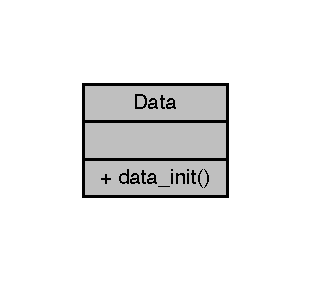
\includegraphics[width=149pt]{class_data__coll__graph}
\end{center}
\end{figure}
\subsubsection*{Offentlige metoder}
\begin{DoxyCompactItemize}
\item 
void \hyperlink{class_data_a68c6d4c829f9363c7d9ff2efbbca50c1}{data\+\_\+init} ()
\begin{DoxyCompactList}\small\item\em Initialiser data modulet. \end{DoxyCompactList}\end{DoxyCompactItemize}


\subsubsection{Detaljeret beskrivelse}
\hyperlink{class_data}{Data} class. 

Indeholder data hentet fra P\+So\+C-\/\+XY, -\/Z og -\/\+Sensor. \begin{DoxyAuthor}{Forfatter}
Jeppe Stærk Antonsen (\href{mailto:201271201@uni.au.dk}{\tt 201271201@uni.\+au.\+dk}) 
\end{DoxyAuthor}


\subsubsection{Dokumentation af medlemsfunktioner}
\index{Data@{Data}!data\+\_\+init@{data\+\_\+init}}
\index{data\+\_\+init@{data\+\_\+init}!Data@{Data}}
\paragraph[{\texorpdfstring{data\+\_\+init()}{data_init()}}]{\setlength{\rightskip}{0pt plus 5cm}void data\+\_\+init (
\begin{DoxyParamCaption}
\item[{void}]{}
\end{DoxyParamCaption}
)}\hypertarget{class_data_a68c6d4c829f9363c7d9ff2efbbca50c1}{}\label{class_data_a68c6d4c829f9363c7d9ff2efbbca50c1}


Initialiser data modulet. 

Initialiser data structen med 0 værdier.

\begin{DoxyAuthor}{Forfatter}
Jeppe Stærk Antonsen (\href{mailto:201271201@uni.au.dk}{\tt 201271201@uni.\+au.\+dk}) 
\end{DoxyAuthor}


Defineret på linje 20 i filen data.\+c.



Indeholder referencer til Data\+Master\+::b\+Val, data\+Master, Data\+Master\+::g\+Val, Data\+Master\+::r\+Val, Data\+Master\+::x\+Val, Data\+Master\+::y\+Val og Data\+Master\+::z\+Val.



Refereret til af main().


\begin{DoxyCode}
21 \{
22   \hyperlink{data_8h_a6b1a8871e30b304a6f5764c44d89e489}{dataMaster}.\hyperlink{data_8h_a7849f509240fa25127fcda8c5009f02b}{xVal} = 0;
23   \hyperlink{data_8h_a6b1a8871e30b304a6f5764c44d89e489}{dataMaster}.\hyperlink{data_8h_a28e89368b5a1aee30ccd952ad63e8c55}{yVal} = 0;
24   \hyperlink{data_8h_a6b1a8871e30b304a6f5764c44d89e489}{dataMaster}.\hyperlink{data_8h_a767a084c35fdc0f1e3e41972d5415483}{zVal} = 0;
25   \hyperlink{data_8h_a6b1a8871e30b304a6f5764c44d89e489}{dataMaster}.\hyperlink{data_8h_a3bf14030a39e71a91c0b97a624f95c5d}{rVal} = 0;
26   \hyperlink{data_8h_a6b1a8871e30b304a6f5764c44d89e489}{dataMaster}.\hyperlink{data_8h_ae02d0c792549f1b88e80ae6eb117f2be}{gVal} = 0;
27   \hyperlink{data_8h_a6b1a8871e30b304a6f5764c44d89e489}{dataMaster}.\hyperlink{data_8h_adf9e1f80891d4eaa914c2bde2502cdf2}{bVal} = 0;
28 \}
\end{DoxyCode}


Her er kalder-\/grafen for denne funktion\+:\nopagebreak
\begin{figure}[H]
\begin{center}
\leavevmode
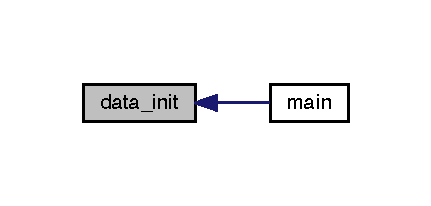
\includegraphics[width=207pt]{class_data_a68c6d4c829f9363c7d9ff2efbbca50c1_icgraph}
\end{center}
\end{figure}




Dokumentationen for denne klasse blev genereret ud fra filerne\+:\begin{DoxyCompactItemize}
\item 
\hyperlink{data_8h}{data.\+h}\item 
\hyperlink{data_8c}{data.\+c}\end{DoxyCompactItemize}

\hypertarget{class_handler}{}\subsection{Handler Klasse-\/reference}
\label{class_handler}\index{Handler@{Handler}}


\hyperlink{class_handler}{Handler} class.  




{\ttfamily \#include $<$handler.\+h$>$}



Samarbejdsdiagram for Handler\+:
\nopagebreak
\begin{figure}[H]
\begin{center}
\leavevmode
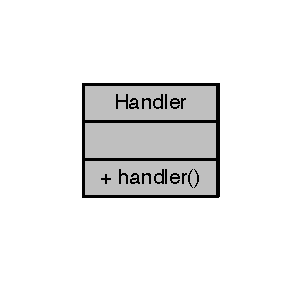
\includegraphics[width=145pt]{d9/de1/class_handler__coll__graph}
\end{center}
\end{figure}
\subsubsection*{Offentlige metoder}
\begin{DoxyCompactItemize}
\item 
void \hyperlink{class_handler_af5be5b016b862943cd22504490acc8f4}{handler} (uint8 cmd, uint8 val)
\begin{DoxyCompactList}\small\item\em Håndter kommando med tilhørende værdi. \end{DoxyCompactList}\end{DoxyCompactItemize}


\subsubsection{Detaljeret beskrivelse}
\hyperlink{class_handler}{Handler} class. 

Håndtere indkommende kommandoer med tilhørende værdier. \begin{DoxyAuthor}{Forfatter}
Jeppe Stærk Antonsen (\href{mailto:201271201@uni.au.dk}{\tt 201271201@uni.\+au.\+dk}) 
\end{DoxyAuthor}


\subsubsection{Dokumentation af medlemsfunktioner}
\index{Handler@{Handler}!handler@{handler}}
\index{handler@{handler}!Handler@{Handler}}
\paragraph[{\texorpdfstring{handler(uint8 cmd, uint8 val)}{handler(uint8 cmd, uint8 val)}}]{\setlength{\rightskip}{0pt plus 5cm}void handler (
\begin{DoxyParamCaption}
\item[{uint8}]{cmd, }
\item[{uint8}]{val}
\end{DoxyParamCaption}
)}\hypertarget{class_handler_af5be5b016b862943cd22504490acc8f4}{}\label{class_handler_af5be5b016b862943cd22504490acc8f4}


Håndter kommando med tilhørende værdi. 

Fortager en defineret handling ud fra den modtaget kommando med den tilhørende værdi. 
\begin{DoxyParams}[1]{Parametre}
\mbox{\tt in}  & {\em cmd} & Er den modtaget kommando. \\
\hline
\mbox{\tt in}  & {\em val} & Er den tilhørende værdi.\\
\hline
\end{DoxyParams}
\begin{DoxyAuthor}{Forfatter}
Jeppe Stærk Antonsen (\href{mailto:201271201@uni.au.dk}{\tt 201271201@uni.\+au.\+dk}) 
\end{DoxyAuthor}


Defineret på linje 26 i filen handler.\+c.



Indeholder referencer til Data\+Master\+::b\+Val, C\+M\+D\+\_\+\+D\+I\+S\+T\+A\+N\+C\+E\+\_\+\+A\+L\+RT, C\+M\+D\+\_\+\+G\+E\+T\+\_\+\+B\+L\+U\+E\+\_\+\+V\+AL, C\+M\+D\+\_\+\+G\+E\+T\+\_\+\+D\+I\+S\+T\+A\+N\+C\+E\+\_\+\+S\+TS, C\+M\+D\+\_\+\+G\+E\+T\+\_\+\+G\+R\+E\+E\+N\+\_\+\+V\+AL, C\+M\+D\+\_\+\+G\+E\+T\+\_\+\+L\+U\+M\+E\+N\+\_\+\+V\+AL, C\+M\+D\+\_\+\+G\+E\+T\+\_\+\+M\+O\+V\+E\+M\+E\+N\+T\+\_\+\+S\+TS, C\+M\+D\+\_\+\+G\+E\+T\+\_\+\+P\+O\+W\+E\+R\+\_\+\+S\+TS, C\+M\+D\+\_\+\+G\+E\+T\+\_\+\+R\+E\+D\+\_\+\+V\+AL, C\+M\+D\+\_\+\+G\+E\+T\+\_\+\+X\+\_\+\+P\+OS, C\+M\+D\+\_\+\+G\+E\+T\+\_\+\+Y\+\_\+\+P\+OS, C\+M\+D\+\_\+\+G\+E\+T\+\_\+\+Z\+\_\+\+P\+OS, C\+M\+D\+\_\+\+M\+O\+V\+E\+M\+E\+N\+T\+\_\+\+A\+L\+RT, C\+M\+D\+\_\+\+S\+E\+T\+\_\+\+B\+L\+U\+E\+\_\+\+V\+AL, C\+M\+D\+\_\+\+S\+E\+T\+\_\+\+D\+I\+S\+T\+A\+N\+C\+E\+\_\+\+S\+TS, C\+M\+D\+\_\+\+S\+E\+T\+\_\+\+G\+R\+E\+E\+N\+\_\+\+V\+AL, C\+M\+D\+\_\+\+S\+E\+T\+\_\+\+L\+U\+M\+E\+N\+\_\+\+V\+AL, C\+M\+D\+\_\+\+S\+E\+T\+\_\+\+M\+O\+V\+E\+M\+E\+N\+T\+\_\+\+S\+TS, C\+M\+D\+\_\+\+S\+E\+T\+\_\+\+P\+O\+W\+E\+R\+\_\+\+S\+TS, C\+M\+D\+\_\+\+S\+E\+T\+\_\+\+R\+E\+D\+\_\+\+V\+AL, C\+M\+D\+\_\+\+S\+E\+T\+\_\+\+X\+\_\+\+P\+OS, C\+M\+D\+\_\+\+S\+E\+T\+\_\+\+Y\+\_\+\+P\+OS, C\+M\+D\+\_\+\+S\+E\+T\+\_\+\+Z\+\_\+\+P\+OS, C\+M\+D\+\_\+\+X\+\_\+\+C\+AL, C\+M\+D\+\_\+\+X\+\_\+\+S\+TP, C\+M\+D\+\_\+\+Y\+\_\+\+C\+AL, C\+M\+D\+\_\+\+Y\+\_\+\+S\+TP, C\+M\+D\+\_\+\+Z\+\_\+\+C\+AL, C\+M\+D\+\_\+\+Z\+\_\+\+S\+TP, data\+Master, Data\+Master\+::g\+Val, I2\+C\+::i2c\+\_\+get\+Packet(), I2\+C\+::i2c\+\_\+set\+Packet(), P\+So\+C\+\_\+\+Sensor, P\+So\+C\+\_\+\+XY, P\+So\+C\+\_\+Z, Data\+Master\+::r\+Val, Data\+Master\+::x\+Val, Data\+Master\+::y\+Val og Data\+Master\+::z\+Val.



Refereret til af main().


\begin{DoxyCode}
27 \{
28   DEBUG\_PutString(\textcolor{stringliteral}{"H=: cmd: "});
29   DEBUG\_PutHexByte(\hyperlink{queue_8h_a85092d82ab6ea85dad51ba78cbda36a0}{cmd});
30   DEBUG\_PutString(\textcolor{stringliteral}{" val: "});
31   DEBUG\_PutHexByte(\hyperlink{queue_8h_aa0ccb5ee6d882ee3605ff47745c6467b}{val});
32   DEBUG\_PutCRLF();
33   
34   \textcolor{keywordflow}{switch} (\hyperlink{queue_8h_a85092d82ab6ea85dad51ba78cbda36a0}{cmd})
35   \{
36     \textcolor{keywordflow}{case} 0x01 :
37       \hyperlink{i2c_8h_afd44ef28b428b7ec2cffb38c97340251}{i2c\_getPacket}(\hyperlink{i2c_8h_a2c70db7df8defae29c1912d84aaee3dc}{PSoC\_XY}, \hyperlink{handler_8h_aa50e083669624eeaef782ebc867008f9}{CMD\_GET\_X\_POS}, &
      \hyperlink{data_8h_a6b1a8871e30b304a6f5764c44d89e489}{dataMaster}.\hyperlink{data_8h_a7849f509240fa25127fcda8c5009f02b}{xVal});
38       \hyperlink{i2c_8h_afd44ef28b428b7ec2cffb38c97340251}{i2c\_getPacket}(\hyperlink{i2c_8h_a2c70db7df8defae29c1912d84aaee3dc}{PSoC\_XY}, \hyperlink{handler_8h_a51053e5251048d6ebbf4d2e23de40761}{CMD\_GET\_Y\_POS}, &
      \hyperlink{data_8h_a6b1a8871e30b304a6f5764c44d89e489}{dataMaster}.\hyperlink{data_8h_a28e89368b5a1aee30ccd952ad63e8c55}{yVal});
39       \hyperlink{i2c_8h_afd44ef28b428b7ec2cffb38c97340251}{i2c\_getPacket}(\hyperlink{i2c_8h_aa72315d85eb390444fdd96475c6aa1f4}{PSoC\_Z}, \hyperlink{handler_8h_a4d76e78d09a00f75609569d9aa92ab98}{CMD\_GET\_Z\_POS}, &
      \hyperlink{data_8h_a6b1a8871e30b304a6f5764c44d89e489}{dataMaster}.\hyperlink{data_8h_a767a084c35fdc0f1e3e41972d5415483}{zVal});
40       \textcolor{keywordflow}{break};
41     \textcolor{keywordflow}{case} 0x03 :
42       \hyperlink{i2c_8h_afd44ef28b428b7ec2cffb38c97340251}{i2c\_getPacket}(\hyperlink{i2c_8h_adc44ca05813864518773ea6f3543816c}{PSoC\_Sensor}, \hyperlink{handler_8h_aa2f09e60c4eeae4560da88c6b1b08c60}{CMD\_GET\_RED\_VAL}, &
      \hyperlink{data_8h_a6b1a8871e30b304a6f5764c44d89e489}{dataMaster}.\hyperlink{data_8h_a3bf14030a39e71a91c0b97a624f95c5d}{rVal});
43       \hyperlink{i2c_8h_afd44ef28b428b7ec2cffb38c97340251}{i2c\_getPacket}(\hyperlink{i2c_8h_adc44ca05813864518773ea6f3543816c}{PSoC\_Sensor}, \hyperlink{handler_8h_a81052c67f996705d7eacfcea66bdde08}{CMD\_GET\_BLUE\_VAL}, &
      \hyperlink{data_8h_a6b1a8871e30b304a6f5764c44d89e489}{dataMaster}.\hyperlink{data_8h_ae02d0c792549f1b88e80ae6eb117f2be}{gVal});
44       \hyperlink{i2c_8h_afd44ef28b428b7ec2cffb38c97340251}{i2c\_getPacket}(\hyperlink{i2c_8h_adc44ca05813864518773ea6f3543816c}{PSoC\_Sensor}, \hyperlink{handler_8h_a55d24f50aeb52afddd491d97a66c81ef}{CMD\_GET\_GREEN\_VAL}, &
      \hyperlink{data_8h_a6b1a8871e30b304a6f5764c44d89e489}{dataMaster}.\hyperlink{data_8h_adf9e1f80891d4eaa914c2bde2502cdf2}{bVal});
45       \textcolor{keywordflow}{break};
46     \textcolor{keywordflow}{case} \hyperlink{handler_8h_af70b73890a98cfe329a916df037f46a4}{CMD\_SET\_X\_POS} :
47       \hyperlink{i2c_8h_a0e13c9c7d87ebdb3680495a787f68d29}{i2c\_setPacket}(\hyperlink{i2c_8h_a2c70db7df8defae29c1912d84aaee3dc}{PSoC\_XY}, \hyperlink{queue_8h_a85092d82ab6ea85dad51ba78cbda36a0}{cmd}, \hyperlink{queue_8h_aa0ccb5ee6d882ee3605ff47745c6467b}{val});
48       \textcolor{keywordflow}{break};
49     \textcolor{keywordflow}{case} \hyperlink{handler_8h_a82640a671f668fb40ff4851901d5a151}{CMD\_SET\_Y\_POS} :
50       \hyperlink{i2c_8h_a0e13c9c7d87ebdb3680495a787f68d29}{i2c\_setPacket}(\hyperlink{i2c_8h_a2c70db7df8defae29c1912d84aaee3dc}{PSoC\_XY}, \hyperlink{queue_8h_a85092d82ab6ea85dad51ba78cbda36a0}{cmd}, \hyperlink{queue_8h_aa0ccb5ee6d882ee3605ff47745c6467b}{val});
51       \textcolor{keywordflow}{break};
52     \textcolor{keywordflow}{case} \hyperlink{handler_8h_aa50e083669624eeaef782ebc867008f9}{CMD\_GET\_X\_POS} :
53       \textcolor{comment}{/* Håndteres i SPI modulet */}
54       \textcolor{keywordflow}{break};
55     \textcolor{keywordflow}{case} \hyperlink{handler_8h_a51053e5251048d6ebbf4d2e23de40761}{CMD\_GET\_Y\_POS} :
56       \textcolor{comment}{/* Håndteres i SPI modulet */}
57       \textcolor{keywordflow}{break};
58     \textcolor{keywordflow}{case} \hyperlink{handler_8h_af7c8f19d1c1b9e2240251d42109c5cfd}{CMD\_X\_STP} :
59       \hyperlink{i2c_8h_a0e13c9c7d87ebdb3680495a787f68d29}{i2c\_setPacket}(\hyperlink{i2c_8h_a2c70db7df8defae29c1912d84aaee3dc}{PSoC\_XY}, \hyperlink{queue_8h_a85092d82ab6ea85dad51ba78cbda36a0}{cmd}, \hyperlink{queue_8h_aa0ccb5ee6d882ee3605ff47745c6467b}{val});
60       \textcolor{keywordflow}{break};
61     \textcolor{keywordflow}{case} \hyperlink{handler_8h_a83ab3037b2c91ea010b2d8c47acd5434}{CMD\_Y\_STP} :
62       \hyperlink{i2c_8h_a0e13c9c7d87ebdb3680495a787f68d29}{i2c\_setPacket}(\hyperlink{i2c_8h_a2c70db7df8defae29c1912d84aaee3dc}{PSoC\_XY}, \hyperlink{queue_8h_a85092d82ab6ea85dad51ba78cbda36a0}{cmd}, \hyperlink{queue_8h_aa0ccb5ee6d882ee3605ff47745c6467b}{val});
63       \textcolor{keywordflow}{break};
64     \textcolor{keywordflow}{case} \hyperlink{handler_8h_a5edf35288955238e1090f2367f96e828}{CMD\_X\_CAL} :
65       \hyperlink{i2c_8h_a0e13c9c7d87ebdb3680495a787f68d29}{i2c\_setPacket}(\hyperlink{i2c_8h_a2c70db7df8defae29c1912d84aaee3dc}{PSoC\_XY}, \hyperlink{queue_8h_a85092d82ab6ea85dad51ba78cbda36a0}{cmd}, \hyperlink{queue_8h_aa0ccb5ee6d882ee3605ff47745c6467b}{val});
66       \textcolor{keywordflow}{break};
67     \textcolor{keywordflow}{case} \hyperlink{handler_8h_a2b2db51eef91dc2aa5586d0817838ef2}{CMD\_Y\_CAL} :
68       \hyperlink{i2c_8h_a0e13c9c7d87ebdb3680495a787f68d29}{i2c\_setPacket}(\hyperlink{i2c_8h_a2c70db7df8defae29c1912d84aaee3dc}{PSoC\_XY}, \hyperlink{queue_8h_a85092d82ab6ea85dad51ba78cbda36a0}{cmd}, \hyperlink{queue_8h_aa0ccb5ee6d882ee3605ff47745c6467b}{val});
69       \textcolor{keywordflow}{break};
70     \textcolor{keywordflow}{case} \hyperlink{handler_8h_a6e695093ea021ccac7cc5d2d788095c9}{CMD\_SET\_Z\_POS} :
71       \hyperlink{i2c_8h_a0e13c9c7d87ebdb3680495a787f68d29}{i2c\_setPacket}(\hyperlink{i2c_8h_aa72315d85eb390444fdd96475c6aa1f4}{PSoC\_Z}, \hyperlink{queue_8h_a85092d82ab6ea85dad51ba78cbda36a0}{cmd}, \hyperlink{queue_8h_aa0ccb5ee6d882ee3605ff47745c6467b}{val});
72       \textcolor{keywordflow}{break};
73     \textcolor{keywordflow}{case} \hyperlink{handler_8h_a4d76e78d09a00f75609569d9aa92ab98}{CMD\_GET\_Z\_POS} :
74       \textcolor{comment}{/* Håndteres i SPI modulet */}
75       \textcolor{keywordflow}{break};
76     \textcolor{keywordflow}{case} \hyperlink{handler_8h_ad119aef78e8cb8e9aa12f35aeae94a99}{CMD\_Z\_STP} :
77       \hyperlink{i2c_8h_a0e13c9c7d87ebdb3680495a787f68d29}{i2c\_setPacket}(\hyperlink{i2c_8h_aa72315d85eb390444fdd96475c6aa1f4}{PSoC\_Z}, \hyperlink{queue_8h_a85092d82ab6ea85dad51ba78cbda36a0}{cmd}, \hyperlink{queue_8h_aa0ccb5ee6d882ee3605ff47745c6467b}{val});
78       \textcolor{keywordflow}{break};
79     \textcolor{keywordflow}{case} \hyperlink{handler_8h_ab77bdaae57e9e34f7bfc1d1a31213f94}{CMD\_Z\_CAL} :
80       \hyperlink{i2c_8h_a0e13c9c7d87ebdb3680495a787f68d29}{i2c\_setPacket}(\hyperlink{i2c_8h_aa72315d85eb390444fdd96475c6aa1f4}{PSoC\_Z}, \hyperlink{queue_8h_a85092d82ab6ea85dad51ba78cbda36a0}{cmd}, \hyperlink{queue_8h_aa0ccb5ee6d882ee3605ff47745c6467b}{val});
81       \textcolor{keywordflow}{break};
82     \textcolor{keywordflow}{case} \hyperlink{handler_8h_afc24de4a99d70315d939185a1c3d61f0}{CMD\_SET\_RED\_VAL} :
83       \hyperlink{i2c_8h_a0e13c9c7d87ebdb3680495a787f68d29}{i2c\_setPacket}(\hyperlink{i2c_8h_adc44ca05813864518773ea6f3543816c}{PSoC\_Sensor}, \hyperlink{queue_8h_a85092d82ab6ea85dad51ba78cbda36a0}{cmd}, \hyperlink{queue_8h_aa0ccb5ee6d882ee3605ff47745c6467b}{val});
84       \textcolor{keywordflow}{break};
85     \textcolor{keywordflow}{case} \hyperlink{handler_8h_a24acd29fea2e546409449638b79ac094}{CMD\_SET\_GREEN\_VAL} :
86       \hyperlink{i2c_8h_a0e13c9c7d87ebdb3680495a787f68d29}{i2c\_setPacket}(\hyperlink{i2c_8h_adc44ca05813864518773ea6f3543816c}{PSoC\_Sensor}, \hyperlink{queue_8h_a85092d82ab6ea85dad51ba78cbda36a0}{cmd}, \hyperlink{queue_8h_aa0ccb5ee6d882ee3605ff47745c6467b}{val});
87       \textcolor{keywordflow}{break};
88     \textcolor{keywordflow}{case} \hyperlink{handler_8h_a4ab3ea64ee56aef3a566698b8959df51}{CMD\_SET\_BLUE\_VAL} :
89       \hyperlink{i2c_8h_a0e13c9c7d87ebdb3680495a787f68d29}{i2c\_setPacket}(\hyperlink{i2c_8h_adc44ca05813864518773ea6f3543816c}{PSoC\_Sensor}, \hyperlink{queue_8h_a85092d82ab6ea85dad51ba78cbda36a0}{cmd}, \hyperlink{queue_8h_aa0ccb5ee6d882ee3605ff47745c6467b}{val});
90       \textcolor{keywordflow}{break};
91     \textcolor{keywordflow}{case} \hyperlink{handler_8h_a3f217d17f4b67e6b46eb294ab3db2e87}{CMD\_SET\_LUMEN\_VAL} :
92       \hyperlink{i2c_8h_a0e13c9c7d87ebdb3680495a787f68d29}{i2c\_setPacket}(\hyperlink{i2c_8h_adc44ca05813864518773ea6f3543816c}{PSoC\_Sensor}, \hyperlink{queue_8h_a85092d82ab6ea85dad51ba78cbda36a0}{cmd}, \hyperlink{queue_8h_aa0ccb5ee6d882ee3605ff47745c6467b}{val});
93       \textcolor{keywordflow}{break};
94     \textcolor{keywordflow}{case} \hyperlink{handler_8h_a1fe6f15c7c98032dc2bd2a1417977fcf}{CMD\_SET\_POWER\_STS} :
95       \hyperlink{i2c_8h_a0e13c9c7d87ebdb3680495a787f68d29}{i2c\_setPacket}(\hyperlink{i2c_8h_adc44ca05813864518773ea6f3543816c}{PSoC\_Sensor}, \hyperlink{queue_8h_a85092d82ab6ea85dad51ba78cbda36a0}{cmd}, \hyperlink{queue_8h_aa0ccb5ee6d882ee3605ff47745c6467b}{val});
96       \textcolor{keywordflow}{break};
97     \textcolor{keywordflow}{case} \hyperlink{handler_8h_aa2f09e60c4eeae4560da88c6b1b08c60}{CMD\_GET\_RED\_VAL} :
98       \textcolor{comment}{/* Håndteres i SPI modulet */}
99       \textcolor{keywordflow}{break};
100     \textcolor{keywordflow}{case} \hyperlink{handler_8h_a55d24f50aeb52afddd491d97a66c81ef}{CMD\_GET\_GREEN\_VAL} :
101       \textcolor{comment}{/* Håndteres i SPI modulet */}
102       \textcolor{keywordflow}{break};
103     \textcolor{keywordflow}{case} \hyperlink{handler_8h_a81052c67f996705d7eacfcea66bdde08}{CMD\_GET\_BLUE\_VAL} :
104       \textcolor{comment}{/* Håndteres i SPI modulet */}
105       \textcolor{keywordflow}{break};
106     \textcolor{keywordflow}{case} \hyperlink{handler_8h_a8ed7ad21a658c878390e9cec4d45aab5}{CMD\_GET\_LUMEN\_VAL} :
107       \textcolor{comment}{/* Håndteres i SPI modulet */}
108       \textcolor{keywordflow}{break};
109     \textcolor{keywordflow}{case} \hyperlink{handler_8h_ab9e8683e41e93fd467b170c321a1c685}{CMD\_GET\_POWER\_STS} :
110       \textcolor{comment}{/* Håndteres i SPI modulet */}
111       \textcolor{keywordflow}{break};
112     \textcolor{keywordflow}{case} \hyperlink{handler_8h_a67cc7e7270e79a6e95be2e25cac29feb}{CMD\_SET\_DISTANCE\_STS} :
113       \hyperlink{i2c_8h_a0e13c9c7d87ebdb3680495a787f68d29}{i2c\_setPacket}(\hyperlink{i2c_8h_adc44ca05813864518773ea6f3543816c}{PSoC\_Sensor}, \hyperlink{queue_8h_a85092d82ab6ea85dad51ba78cbda36a0}{cmd}, \hyperlink{queue_8h_aa0ccb5ee6d882ee3605ff47745c6467b}{val});
114       \textcolor{keywordflow}{break};
115     \textcolor{keywordflow}{case} \hyperlink{handler_8h_a84f8a23b131cb2b163e16889afd9ef85}{CMD\_SET\_MOVEMENT\_STS} :
116       \hyperlink{i2c_8h_a0e13c9c7d87ebdb3680495a787f68d29}{i2c\_setPacket}(\hyperlink{i2c_8h_adc44ca05813864518773ea6f3543816c}{PSoC\_Sensor}, \hyperlink{queue_8h_a85092d82ab6ea85dad51ba78cbda36a0}{cmd}, \hyperlink{queue_8h_aa0ccb5ee6d882ee3605ff47745c6467b}{val});
117       \textcolor{keywordflow}{break};
118     \textcolor{keywordflow}{case} \hyperlink{handler_8h_a8ea17eed84662f9389bfa1751c03a4b2}{CMD\_GET\_DISTANCE\_STS} :
119       \textcolor{comment}{/* Håndteres i SPI modulet */}
120       \textcolor{keywordflow}{break};
121     \textcolor{keywordflow}{case} \hyperlink{handler_8h_a4adcfb68de1b319e19342143cb61b550}{CMD\_GET\_MOVEMENT\_STS} :
122       \textcolor{comment}{/* Håndteres i SPI modulet */}
123       \textcolor{keywordflow}{break};
124     \textcolor{keywordflow}{case} \hyperlink{handler_8h_a17dc606d3dbd6f9d4ca831cb02c91af0}{CMD\_DISTANCE\_ALRT} :
125       \hyperlink{class_handler_af5be5b016b862943cd22504490acc8f4}{handler}(\hyperlink{handler_8h_af7c8f19d1c1b9e2240251d42109c5cfd}{CMD\_X\_STP}, \hyperlink{queue_8h_aa0ccb5ee6d882ee3605ff47745c6467b}{val});
126       \hyperlink{class_handler_af5be5b016b862943cd22504490acc8f4}{handler}(\hyperlink{handler_8h_a83ab3037b2c91ea010b2d8c47acd5434}{CMD\_Y\_STP}, \hyperlink{queue_8h_aa0ccb5ee6d882ee3605ff47745c6467b}{val});
127       \hyperlink{class_handler_af5be5b016b862943cd22504490acc8f4}{handler}(\hyperlink{handler_8h_ad119aef78e8cb8e9aa12f35aeae94a99}{CMD\_Z\_STP}, \hyperlink{queue_8h_aa0ccb5ee6d882ee3605ff47745c6467b}{val});
128       \textcolor{keywordflow}{break};
129     \textcolor{keywordflow}{case} \hyperlink{handler_8h_a7bd43223cfa796f0289d0548e090bbcc}{CMD\_MOVEMENT\_ALRT} :
130       \hyperlink{class_handler_af5be5b016b862943cd22504490acc8f4}{handler}(\hyperlink{handler_8h_a1fe6f15c7c98032dc2bd2a1417977fcf}{CMD\_SET\_POWER\_STS}, \hyperlink{queue_8h_aa0ccb5ee6d882ee3605ff47745c6467b}{val});
131       \textcolor{keywordflow}{break};
132     \textcolor{keywordflow}{default} :
133       \textcolor{keywordflow}{break};
134   \}
135 \}
\end{DoxyCode}


Her er kald-\/grafen for denne funktion\+:
\nopagebreak
\begin{figure}[H]
\begin{center}
\leavevmode
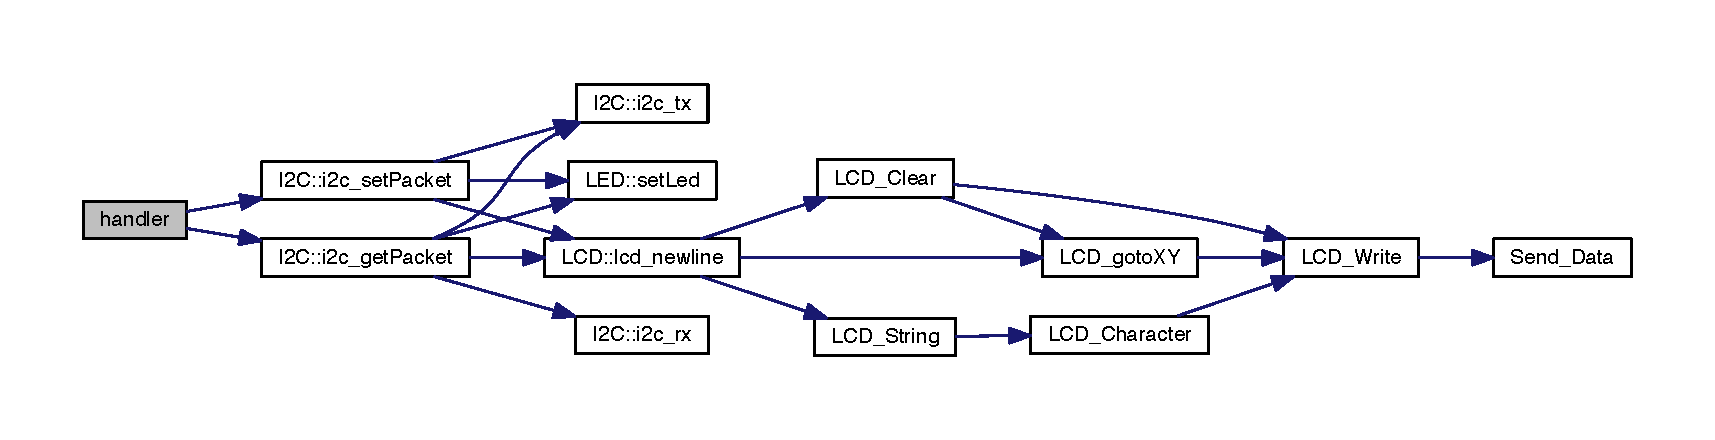
\includegraphics[width=350pt]{d2/d01/class_handler_af5be5b016b862943cd22504490acc8f4_cgraph}
\end{center}
\end{figure}




Her er kalder-\/grafen for denne funktion\+:
\nopagebreak
\begin{figure}[H]
\begin{center}
\leavevmode
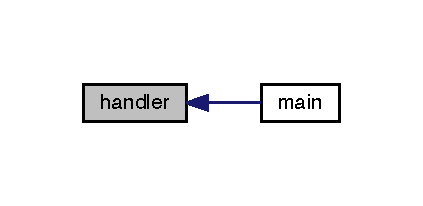
\includegraphics[width=203pt]{d2/d01/class_handler_af5be5b016b862943cd22504490acc8f4_icgraph}
\end{center}
\end{figure}




Dokumentationen for denne klasse blev genereret ud fra filerne\+:\begin{DoxyCompactItemize}
\item 
\hyperlink{handler_8h}{handler.\+h}\item 
\hyperlink{handler_8c}{handler.\+c}\end{DoxyCompactItemize}

\hypertarget{class_i2_c}{}\subsection{I2C Klasse-\/reference}
\label{class_i2_c}\index{I2C@{I2C}}


\hyperlink{class_i2_c}{I2C} class.  




{\ttfamily \#include $<$i2c.\+h$>$}



Samarbejdsdiagram for I2C\+:
\nopagebreak
\begin{figure}[H]
\begin{center}
\leavevmode
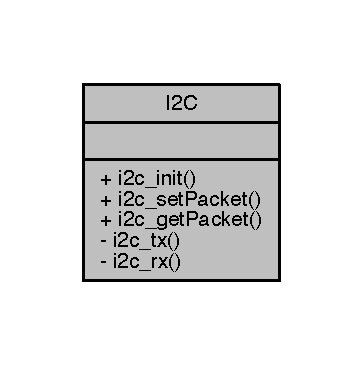
\includegraphics[width=237pt]{df/d70/class_i2_c__coll__graph}
\end{center}
\end{figure}
\subsubsection*{Offentlige metoder}
\begin{DoxyCompactItemize}
\item 
void \hyperlink{class_i2_c_a64303230bf4843297e7ac37ac236ca04}{i2c\+\_\+init} ()
\begin{DoxyCompactList}\small\item\em Initialiser \hyperlink{class_i2_c}{I2C} modulet. \end{DoxyCompactList}\item 
void \hyperlink{class_i2_c_a1b75ff104f3614357d14cee6514ad108}{I2\+C\+S\+\_\+\+I2\+C\+\_\+\+I\+S\+R\+\_\+\+Exit\+Callback} ()
\begin{DoxyCompactList}\small\item\em Motager \char`\"{}\+Exit Callback\char`\"{} fra \hyperlink{class_i2_c}{I2C}. \end{DoxyCompactList}\item 
void \hyperlink{class_i2_c_a3d3187ad377a6ca29b3fac5c809b6012}{i2c\+\_\+tx} ()
\begin{DoxyCompactList}\small\item\em Ryder om efter \hyperlink{class_i2_c}{I2C}. \end{DoxyCompactList}\item 
uint8 \hyperlink{class_i2_c_a58ba88cddd7843f12a40a87c998f00da}{i2c\+Tx\+Buffer} \mbox{[}\hyperlink{i2c_8h_a6458dbf193a0eef0470fc1b08400bfcd}{I2\+C\+\_\+\+B\+U\+F\+F\+E\+R\+\_\+\+S\+I\+ZE}\mbox{]}
\begin{DoxyCompactList}\small\item\em Buffer til afsendelse af data. \end{DoxyCompactList}\item 
uint8 \hyperlink{class_i2_c_a711782550427eea544dabe5394d79a9b}{i2c\+Rx\+Buffer} \mbox{[}\hyperlink{i2c_8h_a6458dbf193a0eef0470fc1b08400bfcd}{I2\+C\+\_\+\+B\+U\+F\+F\+E\+R\+\_\+\+S\+I\+ZE}\mbox{]}
\begin{DoxyCompactList}\small\item\em Buffer til modtagelse af data. \end{DoxyCompactList}\end{DoxyCompactItemize}
\subsubsection*{Private attributter}
\begin{DoxyCompactItemize}
\item 
uint8 \hyperlink{class_i2_c_af66ed5dc7817e74d7da731c994721217}{i2c\+Tx\+Buffer} \mbox{[}\hyperlink{i2c_8h_a6458dbf193a0eef0470fc1b08400bfcd}{I2\+C\+\_\+\+B\+U\+F\+F\+E\+R\+\_\+\+S\+I\+ZE}\mbox{]} = \{\hyperlink{i2c_8h_a52bb5b964361ed2f1b18df32c5b8f2c5}{I2\+C\+\_\+\+P\+A\+C\+K\+E\+T\+\_\+\+S\+OP}, \hyperlink{i2c_8h_aee0adbd7dcb13e95337369b7342a27e3}{I2\+C\+\_\+\+S\+T\+S\+\_\+\+C\+M\+D\+\_\+\+F\+A\+IL}, \hyperlink{i2c_8h_aee0adbd7dcb13e95337369b7342a27e3}{I2\+C\+\_\+\+S\+T\+S\+\_\+\+C\+M\+D\+\_\+\+F\+A\+IL}, \hyperlink{i2c_8h_a62b4ae6e51a3d0da47f5165165cdbc0a}{I2\+C\+\_\+\+P\+A\+C\+K\+E\+T\+\_\+\+E\+OP}\}
\begin{DoxyCompactList}\small\item\em Buffer til afsendelse af data. \end{DoxyCompactList}\item 
uint8 \hyperlink{class_i2_c_a88d6ebcf1ef5f528b63cf306ad1a5909}{i2c\+Rx\+Buffer} \mbox{[}\hyperlink{i2c_8h_a6458dbf193a0eef0470fc1b08400bfcd}{I2\+C\+\_\+\+B\+U\+F\+F\+E\+R\+\_\+\+S\+I\+ZE}\mbox{]}
\begin{DoxyCompactList}\small\item\em Buffer til modtagelse af data. \end{DoxyCompactList}\end{DoxyCompactItemize}


\subsubsection{Detaljeret beskrivelse}
\hyperlink{class_i2_c}{I2C} class. 

Håndter kommunikation via I2\+C-\/busset. \begin{DoxyAuthor}{Forfatter}
Jeppe Stærk Antonsen (\href{mailto:201271201@uni.au.dk}{\tt 201271201@uni.\+au.\+dk}) 
\end{DoxyAuthor}


\subsubsection{Dokumentation af medlemsfunktioner}
\index{I2C@{I2C}!i2c\+\_\+init@{i2c\+\_\+init}}
\index{i2c\+\_\+init@{i2c\+\_\+init}!I2C@{I2C}}
\paragraph[{\texorpdfstring{i2c\+\_\+init()}{i2c_init()}}]{\setlength{\rightskip}{0pt plus 5cm}void i2c\+\_\+init (
\begin{DoxyParamCaption}
\item[{void}]{}
\end{DoxyParamCaption}
)}\hypertarget{class_i2_c_a64303230bf4843297e7ac37ac236ca04}{}\label{class_i2_c_a64303230bf4843297e7ac37ac236ca04}


Initialiser \hyperlink{class_i2_c}{I2C} modulet. 

Initailiser \hyperlink{class_i2_c}{I2C} komponent på P\+SoC\textquotesingle{}en.

\begin{DoxyAuthor}{Forfatter}
Jeppe Stærk (\href{mailto:201271201@uni.au.dk}{\tt 201271201@uni.\+au.\+dk}) 
\end{DoxyAuthor}


Defineret på linje 49 i filen i2c.\+c.



Indeholder referencer til I2\+C\+\_\+\+B\+U\+F\+F\+E\+R\+\_\+\+S\+I\+ZE, i2c\+Rx\+Buffer() og i2c\+Tx\+Buffer().



Refereret til af main().


\begin{DoxyCode}
50 \{
51   I2CS\_I2CSlaveInitReadBuf(\hyperlink{class_i2_c_a58ba88cddd7843f12a40a87c998f00da}{i2cTxBuffer}, \hyperlink{i2c_8h_a6458dbf193a0eef0470fc1b08400bfcd}{I2C\_BUFFER\_SIZE});
52   I2CS\_I2CSlaveClearReadBuf();
53   I2CS\_I2CSlaveClearReadStatus();
54   
55   I2CS\_I2CSlaveInitWriteBuf(\hyperlink{class_i2_c_a711782550427eea544dabe5394d79a9b}{i2cRxBuffer}, \hyperlink{i2c_8h_a6458dbf193a0eef0470fc1b08400bfcd}{I2C\_BUFFER\_SIZE});
56   I2CS\_I2CSlaveClearWriteBuf();
57   I2CS\_I2CSlaveClearWriteStatus();
58   
59   I2CS\_Start();
60 \}
\end{DoxyCode}


Her er kald-\/grafen for denne funktion\+:
\nopagebreak
\begin{figure}[H]
\begin{center}
\leavevmode
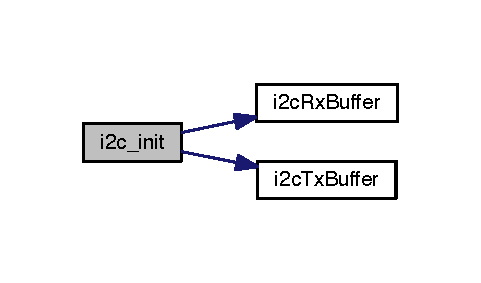
\includegraphics[width=231pt]{d4/d47/class_i2_c_a64303230bf4843297e7ac37ac236ca04_cgraph}
\end{center}
\end{figure}




Her er kalder-\/grafen for denne funktion\+:
\nopagebreak
\begin{figure}[H]
\begin{center}
\leavevmode
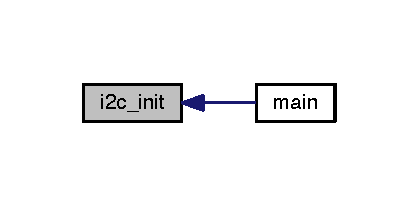
\includegraphics[width=201pt]{d4/d47/class_i2_c_a64303230bf4843297e7ac37ac236ca04_icgraph}
\end{center}
\end{figure}


\index{I2C@{I2C}!i2c\+\_\+tx@{i2c\+\_\+tx}}
\index{i2c\+\_\+tx@{i2c\+\_\+tx}!I2C@{I2C}}
\paragraph[{\texorpdfstring{i2c\+\_\+tx()}{i2c_tx()}}]{\setlength{\rightskip}{0pt plus 5cm}void i2c\+\_\+tx (
\begin{DoxyParamCaption}
\item[{void}]{}
\end{DoxyParamCaption}
)}\hypertarget{class_i2_c_a3d3187ad377a6ca29b3fac5c809b6012}{}\label{class_i2_c_a3d3187ad377a6ca29b3fac5c809b6012}


Ryder om efter \hyperlink{class_i2_c}{I2C}. 

Efter fuldført afsendelse af pakke til I2\+C-\/master, bliver status nulstillet.

\begin{DoxyAuthor}{Forfatter}
Jeppe Stærk (\href{mailto:201271201@uni.au.dk}{\tt 201271201@uni.\+au.\+dk}) 
\end{DoxyAuthor}


Defineret på linje 115 i filen i2c.\+c.



Refereret til af main().


\begin{DoxyCode}
116 \{
117   \textcolor{keywordflow}{if}(0u != (I2CS\_I2CSlaveStatus() & I2CS\_I2C\_SSTAT\_RD\_CMPLT))
118   \{
119     I2CS\_I2CSlaveClearReadBuf();
120     (void) I2CS\_I2CSlaveClearReadStatus();
121   \}
122 \}
\end{DoxyCode}


Her er kalder-\/grafen for denne funktion\+:
\nopagebreak
\begin{figure}[H]
\begin{center}
\leavevmode
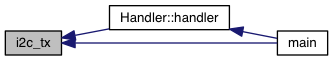
\includegraphics[width=196pt]{d4/d47/class_i2_c_a3d3187ad377a6ca29b3fac5c809b6012_icgraph}
\end{center}
\end{figure}


\index{I2C@{I2C}!i2c\+Rx\+Buffer@{i2c\+Rx\+Buffer}}
\index{i2c\+Rx\+Buffer@{i2c\+Rx\+Buffer}!I2C@{I2C}}
\paragraph[{\texorpdfstring{i2c\+Rx\+Buffer[I2\+C\+\_\+\+B\+U\+F\+F\+E\+R\+\_\+\+S\+I\+ZE]}{i2cRxBuffer[I2C_BUFFER_SIZE]}}]{\setlength{\rightskip}{0pt plus 5cm}uint8 i2c\+Rx\+Buffer (
\begin{DoxyParamCaption}
{}
\end{DoxyParamCaption}
)}\hypertarget{class_i2_c_a711782550427eea544dabe5394d79a9b}{}\label{class_i2_c_a711782550427eea544dabe5394d79a9b}


Buffer til modtagelse af data. 

En buffer der indeholder de data pakker der skal modtagelse over I2\+C-\/busset.

\begin{DoxyAuthor}{Forfatter}
Jeppe Stærk (\href{mailto:201271201@uni.au.dk}{\tt 201271201@uni.\+au.\+dk}) 
\end{DoxyAuthor}


Defineret på linje 76 i filen i2c.\+h.



Refereret til af i2c\+\_\+init() og I2\+C\+S\+\_\+\+I2\+C\+\_\+\+I\+S\+R\+\_\+\+Exit\+Callback().



Her er kalder-\/grafen for denne funktion\+:
\nopagebreak
\begin{figure}[H]
\begin{center}
\leavevmode
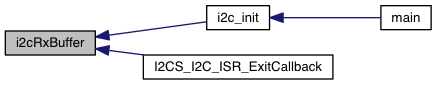
\includegraphics[width=350pt]{d4/d47/class_i2_c_a711782550427eea544dabe5394d79a9b_icgraph}
\end{center}
\end{figure}


\index{I2C@{I2C}!I2\+C\+S\+\_\+\+I2\+C\+\_\+\+I\+S\+R\+\_\+\+Exit\+Callback@{I2\+C\+S\+\_\+\+I2\+C\+\_\+\+I\+S\+R\+\_\+\+Exit\+Callback}}
\index{I2\+C\+S\+\_\+\+I2\+C\+\_\+\+I\+S\+R\+\_\+\+Exit\+Callback@{I2\+C\+S\+\_\+\+I2\+C\+\_\+\+I\+S\+R\+\_\+\+Exit\+Callback}!I2C@{I2C}}
\paragraph[{\texorpdfstring{I2\+C\+S\+\_\+\+I2\+C\+\_\+\+I\+S\+R\+\_\+\+Exit\+Callback()}{I2CS_I2C_ISR_ExitCallback()}}]{\setlength{\rightskip}{0pt plus 5cm}void I2\+C\+S\+\_\+\+I2\+C\+\_\+\+I\+S\+R\+\_\+\+Exit\+Callback (
\begin{DoxyParamCaption}
\item[{void}]{}
\end{DoxyParamCaption}
)}\hypertarget{class_i2_c_a1b75ff104f3614357d14cee6514ad108}{}\label{class_i2_c_a1b75ff104f3614357d14cee6514ad108}


Motager \char`\"{}\+Exit Callback\char`\"{} fra \hyperlink{class_i2_c}{I2C}. 

En \char`\"{}\+Interrupt Service Routine(\+I\+S\+R)\char`\"{} der aktiveres ved færdig modtagelse af kald via I2\+C-\/busset, det modtaget data behandles og håndteres.

\begin{DoxyAuthor}{Forfatter}
Jeppe Stærk (\href{mailto:201271201@uni.au.dk}{\tt 201271201@uni.\+au.\+dk}) 
\end{DoxyAuthor}


Defineret på linje 69 i filen i2c.\+c.



Indeholder referencer til Action\+::cmd, C\+M\+D\+\_\+\+S\+E\+T\+\_\+\+Z\+\_\+\+P\+OS, dataZ, I2\+C\+\_\+\+B\+U\+F\+F\+E\+R\+\_\+\+S\+I\+ZE, I2\+C\+\_\+\+P\+A\+C\+K\+E\+T\+\_\+\+C\+M\+D\+\_\+\+P\+OS, I2\+C\+\_\+\+P\+A\+C\+K\+E\+T\+\_\+\+V\+A\+L\+\_\+\+P\+OS, i2c\+Rx\+Buffer(), Data\+Z\+::isr\+StopZ, Queue\+::push\+Queue() og Action\+::val.


\begin{DoxyCode}
70 \{
71   \textcolor{keywordflow}{if}(I2CS\_I2CSlaveGetWriteBufSize() == \hyperlink{i2c_8h_a6458dbf193a0eef0470fc1b08400bfcd}{I2C\_BUFFER\_SIZE})
72   \{
73     DEBUG\_PutCRLF();
74     DEBUG\_PutString(\textcolor{stringliteral}{"** isr exit callback **"});
75     DEBUG\_PutCRLF();
76     DEBUG\_PutString(\textcolor{stringliteral}{"I> i2cRxBuffer[0]: "});
77     DEBUG\_PutHexByte(\hyperlink{class_i2_c_a711782550427eea544dabe5394d79a9b}{i2cRxBuffer}[0]);
78     DEBUG\_PutString(\textcolor{stringliteral}{" [1]: "});
79     DEBUG\_PutHexByte(\hyperlink{class_i2_c_a711782550427eea544dabe5394d79a9b}{i2cRxBuffer}[1]);
80     DEBUG\_PutString(\textcolor{stringliteral}{" [2]: "});
81     DEBUG\_PutHexByte(\hyperlink{class_i2_c_a711782550427eea544dabe5394d79a9b}{i2cRxBuffer}[2]);
82     DEBUG\_PutString(\textcolor{stringliteral}{" [3]: "});
83     DEBUG\_PutHexByte(\hyperlink{class_i2_c_a711782550427eea544dabe5394d79a9b}{i2cRxBuffer}[3]);
84     DEBUG\_PutString(\textcolor{stringliteral}{" buffer size: "});
85     DEBUG\_PutHexByte(I2CS\_I2CSlaveGetWriteBufSize());
86     DEBUG\_PutCRLF();
87     
88     \textcolor{keyword}{struct }\hyperlink{queue_8h_df/d8c/struct_action}{Action} action;
89     action.\hyperlink{queue_8h_a85092d82ab6ea85dad51ba78cbda36a0}{cmd} = \hyperlink{class_i2_c_a711782550427eea544dabe5394d79a9b}{i2cRxBuffer}[\hyperlink{i2c_8h_ac13fcfeded7dc2d82fa4734456f3761f}{I2C\_PACKET\_CMD\_POS}];
90     action.val = \hyperlink{class_i2_c_a711782550427eea544dabe5394d79a9b}{i2cRxBuffer}[\hyperlink{i2c_8h_a68506c3651f015716bb2c135e8e7b972}{I2C\_PACKET\_VAL\_POS}];
91     
92     \textcolor{keywordflow}{switch}(\hyperlink{class_i2_c_a711782550427eea544dabe5394d79a9b}{i2cRxBuffer}[\hyperlink{i2c_8h_ac13fcfeded7dc2d82fa4734456f3761f}{I2C\_PACKET\_CMD\_POS}]) \{
93       \textcolor{keywordflow}{case} \hyperlink{handler_8h_a6e695093ea021ccac7cc5d2d788095c9}{CMD\_SET\_Z\_POS} :
94         \hyperlink{data_8h_ace1aa5b973b9358f7236c0c9deca9370}{dataZ}.\hyperlink{data_8h_ae55ff8378d0a07b118000a98b273141f}{isrStopZ} = 1;
95         DEBUG\_PutString(\textcolor{stringliteral}{") isrStopZ = 1"});
96         DEBUG\_PutCRLF();
97         \hyperlink{queue_8h_a0012fa831aa1529e5ed3a6610b733423}{pushQueue}(action);
98         \textcolor{keywordflow}{break};
99       \textcolor{keywordflow}{default} :
100         \hyperlink{queue_8h_a0012fa831aa1529e5ed3a6610b733423}{pushQueue}(action);
101         \textcolor{keywordflow}{break};
102     \}
103     I2CS\_I2CSlaveClearWriteBuf();
104     (void) I2CS\_I2CSlaveClearWriteStatus();
105   \}
106 \}
\end{DoxyCode}


Her er kald-\/grafen for denne funktion\+:
\nopagebreak
\begin{figure}[H]
\begin{center}
\leavevmode
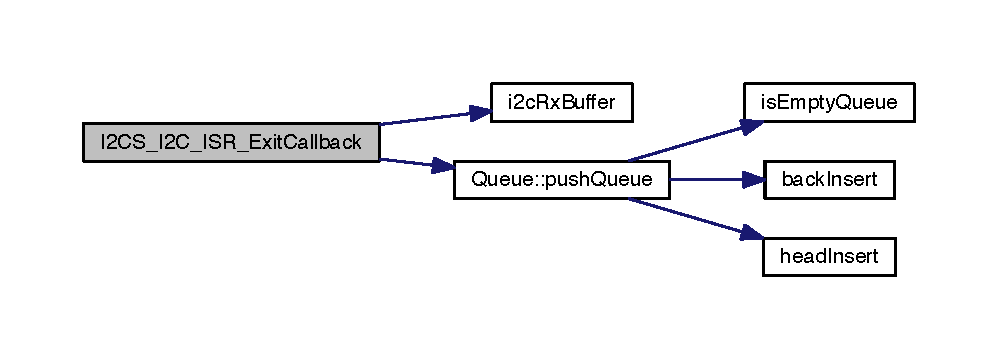
\includegraphics[width=350pt]{d4/d47/class_i2_c_a1b75ff104f3614357d14cee6514ad108_cgraph}
\end{center}
\end{figure}


\index{I2C@{I2C}!i2c\+Tx\+Buffer@{i2c\+Tx\+Buffer}}
\index{i2c\+Tx\+Buffer@{i2c\+Tx\+Buffer}!I2C@{I2C}}
\paragraph[{\texorpdfstring{i2c\+Tx\+Buffer[I2\+C\+\_\+\+B\+U\+F\+F\+E\+R\+\_\+\+S\+I\+ZE]}{i2cTxBuffer[I2C_BUFFER_SIZE]}}]{\setlength{\rightskip}{0pt plus 5cm}uint8 i2c\+Tx\+Buffer (
\begin{DoxyParamCaption}
{}
\end{DoxyParamCaption}
)}\hypertarget{class_i2_c_a58ba88cddd7843f12a40a87c998f00da}{}\label{class_i2_c_a58ba88cddd7843f12a40a87c998f00da}


Buffer til afsendelse af data. 

En buffer der indeholder de data pakker der skal sende over I2\+C-\/busset.

\begin{DoxyAuthor}{Forfatter}
Jeppe Stærk (\href{mailto:201271201@uni.au.dk}{\tt 201271201@uni.\+au.\+dk}) 
\end{DoxyAuthor}


Defineret på linje 67 i filen i2c.\+h.



Refereret til af Handler\+::handler() og i2c\+\_\+init().



Her er kalder-\/grafen for denne funktion\+:
\nopagebreak
\begin{figure}[H]
\begin{center}
\leavevmode
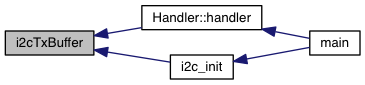
\includegraphics[width=346pt]{d4/d47/class_i2_c_a58ba88cddd7843f12a40a87c998f00da_icgraph}
\end{center}
\end{figure}




\subsubsection{Felt-\/dokumentation}
\index{I2C@{I2C}!i2c\+Rx\+Buffer@{i2c\+Rx\+Buffer}}
\index{i2c\+Rx\+Buffer@{i2c\+Rx\+Buffer}!I2C@{I2C}}
\paragraph[{\texorpdfstring{i2c\+Rx\+Buffer}{i2cRxBuffer}}]{\setlength{\rightskip}{0pt plus 5cm}uint8 i2c\+Rx\+Buffer\mbox{[}{\bf I2\+C\+\_\+\+B\+U\+F\+F\+E\+R\+\_\+\+S\+I\+ZE}\mbox{]}\hspace{0.3cm}{\ttfamily [private]}}\hypertarget{class_i2_c_a88d6ebcf1ef5f528b63cf306ad1a5909}{}\label{class_i2_c_a88d6ebcf1ef5f528b63cf306ad1a5909}


Buffer til modtagelse af data. 

En buffer der indeholder de data pakker der skal modtagelse over I2\+C-\/busset.

\begin{DoxyAuthor}{Forfatter}
Jeppe Stærk (\href{mailto:201271201@uni.au.dk}{\tt 201271201@uni.\+au.\+dk}) 
\end{DoxyAuthor}


Defineret på linje 35 i filen i2c.\+c.

\index{I2C@{I2C}!i2c\+Tx\+Buffer@{i2c\+Tx\+Buffer}}
\index{i2c\+Tx\+Buffer@{i2c\+Tx\+Buffer}!I2C@{I2C}}
\paragraph[{\texorpdfstring{i2c\+Tx\+Buffer}{i2cTxBuffer}}]{\setlength{\rightskip}{0pt plus 5cm}uint8 i2c\+Tx\+Buffer\mbox{[}{\bf I2\+C\+\_\+\+B\+U\+F\+F\+E\+R\+\_\+\+S\+I\+ZE}\mbox{]} = \{{\bf I2\+C\+\_\+\+P\+A\+C\+K\+E\+T\+\_\+\+S\+OP}, {\bf I2\+C\+\_\+\+S\+T\+S\+\_\+\+C\+M\+D\+\_\+\+F\+A\+IL}, {\bf I2\+C\+\_\+\+S\+T\+S\+\_\+\+C\+M\+D\+\_\+\+F\+A\+IL}, {\bf I2\+C\+\_\+\+P\+A\+C\+K\+E\+T\+\_\+\+E\+OP}\}\hspace{0.3cm}{\ttfamily [private]}}\hypertarget{class_i2_c_af66ed5dc7817e74d7da731c994721217}{}\label{class_i2_c_af66ed5dc7817e74d7da731c994721217}


Buffer til afsendelse af data. 

En buffer der indeholder de data pakker der skal sende over I2\+C-\/busset.

\begin{DoxyAuthor}{Forfatter}
Jeppe Stærk (\href{mailto:201271201@uni.au.dk}{\tt 201271201@uni.\+au.\+dk}) 
\end{DoxyAuthor}


Defineret på linje 26 i filen i2c.\+c.



Dokumentationen for denne klasse blev genereret ud fra filerne\+:\begin{DoxyCompactItemize}
\item 
\hyperlink{i2c_8h}{i2c.\+h}\item 
\hyperlink{i2c_8c}{i2c.\+c}\end{DoxyCompactItemize}

\hypertarget{class_l_c_d}{}\subsection{L\+CD Klasse-\/reference}
\label{class_l_c_d}\index{L\+CD@{L\+CD}}


\hyperlink{class_l_c_d}{L\+CD} class.  




{\ttfamily \#include $<$lcd.\+h$>$}



Samarbejdsdiagram for L\+CD\+:
\nopagebreak
\begin{figure}[H]
\begin{center}
\leavevmode
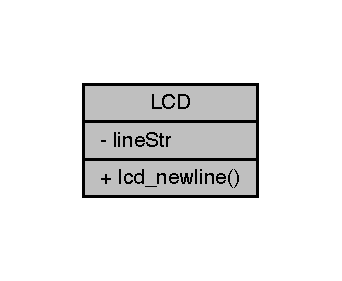
\includegraphics[width=164pt]{d2/dbd/class_l_c_d__coll__graph}
\end{center}
\end{figure}
\subsubsection*{Offentlige metoder}
\begin{DoxyCompactItemize}
\item 
void \hyperlink{class_l_c_d_a507dd352aee8161dc556e3d1439a2be2}{lcd\+\_\+newline} (char $\ast$characters)
\begin{DoxyCompactList}\small\item\em Udskriver tekst på Nokia 5110 \hyperlink{class_l_c_d}{L\+CD}. \end{DoxyCompactList}\end{DoxyCompactItemize}
\subsubsection*{Private attributter}
\begin{DoxyCompactItemize}
\item 
char \hyperlink{class_l_c_d_a51a220275e6d21942189276ef7d9e7c3}{line\+Str} \mbox{[}6\mbox{]}\mbox{[}12\mbox{]}
\begin{DoxyCompactList}\small\item\em Char array der indholder tekst. \end{DoxyCompactList}\end{DoxyCompactItemize}


\subsubsection{Detaljeret beskrivelse}
\hyperlink{class_l_c_d}{L\+CD} class. 

Sender tekst til Nokia5110\+L\+CD skærmen via dens eksterne kode. \begin{DoxyAuthor}{Forfatter}
Jeppe Stærk Antonsen (\href{mailto:201271201@uni.au.dk}{\tt 201271201@uni.\+au.\+dk}) 
\end{DoxyAuthor}


\subsubsection{Dokumentation af medlemsfunktioner}
\index{L\+CD@{L\+CD}!lcd\+\_\+newline@{lcd\+\_\+newline}}
\index{lcd\+\_\+newline@{lcd\+\_\+newline}!L\+CD@{L\+CD}}
\paragraph[{\texorpdfstring{lcd\+\_\+newline(char $\ast$characters)}{lcd_newline(char *characters)}}]{\setlength{\rightskip}{0pt plus 5cm}void lcd\+\_\+newline (
\begin{DoxyParamCaption}
\item[{char $\ast$}]{characters}
\end{DoxyParamCaption}
)}\hypertarget{class_l_c_d_a507dd352aee8161dc556e3d1439a2be2}{}\label{class_l_c_d_a507dd352aee8161dc556e3d1439a2be2}


Udskriver tekst på Nokia 5110 \hyperlink{class_l_c_d}{L\+CD}. 

Metoden bruges til at skrive en ny linje nederst på Nokia 5110 \hyperlink{class_l_c_d}{L\+CD} skærmen, den husker på-\/ og flytter de forhenværende linjer en linje op, når der indættes en ny.

\begin{DoxyAuthor}{Forfatter}
Jeppe Stærk (\href{mailto:201271201@uni.au.dk}{\tt 201271201@uni.\+au.\+dk}) 
\end{DoxyAuthor}


Defineret på linje 36 i filen lcd.\+c.



Indeholder referencer til L\+C\+D\+\_\+\+Clear(), L\+C\+D\+\_\+goto\+X\+Y(), L\+C\+D\+\_\+\+String() og line\+Str.



Refereret til af S\+P\+I\+::\+C\+Y\+\_\+\+I\+S\+R(), I2\+C\+::i2c\+\_\+get\+Packet(), I2\+C\+::i2c\+\_\+set\+Packet() og main().


\begin{DoxyCode}
37 \{
38   \textcolor{keywordtype}{int} i;
39   
40   \textcolor{keywordflow}{for}(i = 0; i < 5; i++)
41   \{
42     strncpy(\hyperlink{class_l_c_d_a51a220275e6d21942189276ef7d9e7c3}{lineStr}[i],\hyperlink{class_l_c_d_a51a220275e6d21942189276ef7d9e7c3}{lineStr}[i+1],12);
43   \}
44   
45   strcpy(\hyperlink{class_l_c_d_a51a220275e6d21942189276ef7d9e7c3}{lineStr}[5], characters);
46   
47   \hyperlink{_nokia5110_l_c_d_8c_ae60d0b62d7eb3fa31266c095d7b3c245}{LCD\_Clear}();
48   \textcolor{keywordflow}{for}(i = 0; i < 6; i++)
49   \{
50     \hyperlink{_nokia5110_l_c_d_8c_adde1a4c2e7bd6bc1bbeb7694db45925b}{LCD\_gotoXY}(0,i);
51     \hyperlink{_nokia5110_l_c_d_8c_a4c2c90307f23817e8445be5c6ca537c5}{LCD\_String}(\hyperlink{class_l_c_d_a51a220275e6d21942189276ef7d9e7c3}{lineStr}[i]);
52   \}
53 \}
\end{DoxyCode}


Her er kald-\/grafen for denne funktion\+:
\nopagebreak
\begin{figure}[H]
\begin{center}
\leavevmode
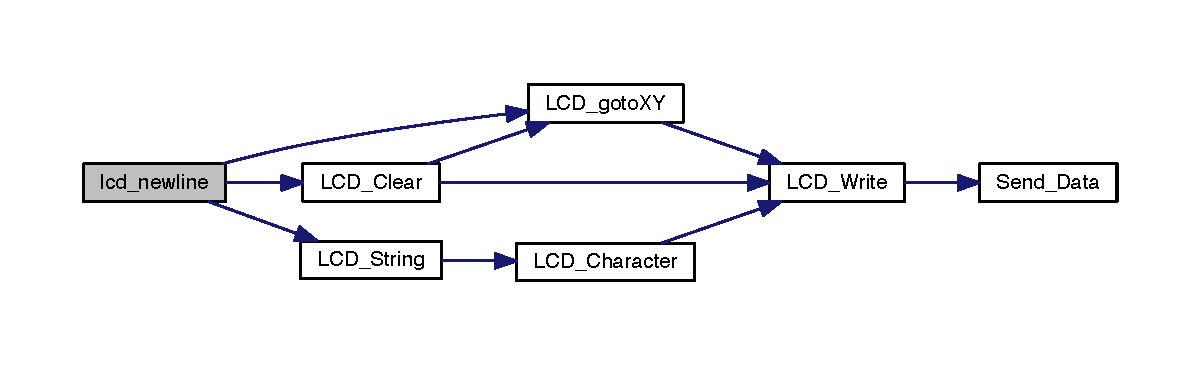
\includegraphics[width=350pt]{df/dd6/class_l_c_d_a507dd352aee8161dc556e3d1439a2be2_cgraph}
\end{center}
\end{figure}




Her er kalder-\/grafen for denne funktion\+:
\nopagebreak
\begin{figure}[H]
\begin{center}
\leavevmode
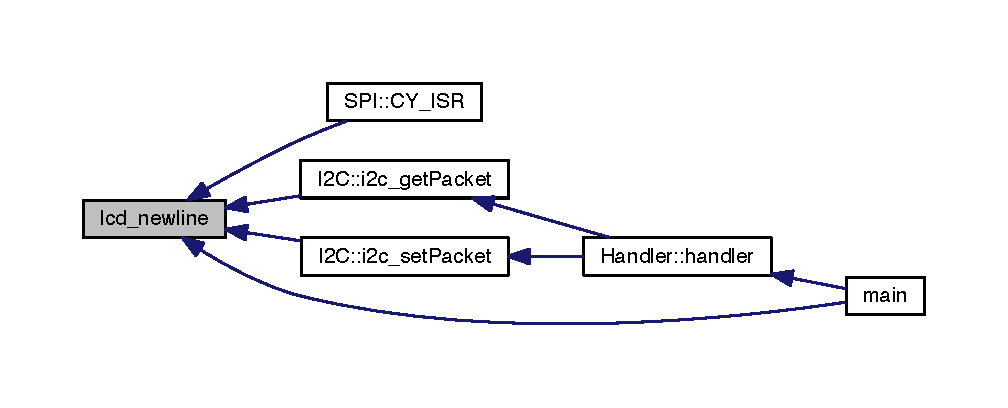
\includegraphics[width=350pt]{df/dd6/class_l_c_d_a507dd352aee8161dc556e3d1439a2be2_icgraph}
\end{center}
\end{figure}




\subsubsection{Felt-\/dokumentation}
\index{L\+CD@{L\+CD}!line\+Str@{line\+Str}}
\index{line\+Str@{line\+Str}!L\+CD@{L\+CD}}
\paragraph[{\texorpdfstring{line\+Str}{lineStr}}]{\setlength{\rightskip}{0pt plus 5cm}char line\+Str\mbox{[}6\mbox{]}\mbox{[}12\mbox{]}\hspace{0.3cm}{\ttfamily [private]}}\hypertarget{class_l_c_d_a51a220275e6d21942189276ef7d9e7c3}{}\label{class_l_c_d_a51a220275e6d21942189276ef7d9e7c3}


Char array der indholder tekst. 

Arrayet er et matrix array med 6 arryes med 12 pladser, det bruges til at indeholde de 6 linjer tekst der kan udskrives på Nokia 5110 \hyperlink{class_l_c_d}{L\+CD} skærmen.

\begin{DoxyAuthor}{Forfatter}
Jeppe Stærk (\href{mailto:201271201@uni.au.dk}{\tt 201271201@uni.\+au.\+dk}) 
\end{DoxyAuthor}


Defineret på linje 22 i filen lcd.\+c.



Refereret til af lcd\+\_\+newline().



Dokumentationen for denne klasse blev genereret ud fra filerne\+:\begin{DoxyCompactItemize}
\item 
\hyperlink{lcd_8h}{lcd.\+h}\item 
\hyperlink{lcd_8c}{lcd.\+c}\end{DoxyCompactItemize}

\hypertarget{class_l_e_d}{}\subsection{L\+ED Klasse-\/reference}
\label{class_l_e_d}\index{L\+ED@{L\+ED}}


\hyperlink{class_l_e_d}{L\+ED} class.  




{\ttfamily \#include $<$led.\+h$>$}



Samarbejdsdiagram for L\+ED\+:\nopagebreak
\begin{figure}[H]
\begin{center}
\leavevmode
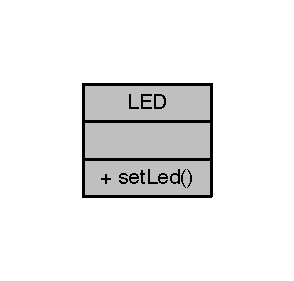
\includegraphics[width=141pt]{d3/df9/class_l_e_d__coll__graph}
\end{center}
\end{figure}
\subsubsection*{Offentlige metoder}
\begin{DoxyCompactItemize}
\item 
void \hyperlink{class_l_e_d_a1d8e725e3829da99c1d027ba0a2ce57a}{set\+Led} (uint8 red, uint8 green, uint8 blue, uint8 delay)
\begin{DoxyCompactList}\small\item\em Sætter den defineret farve og angivet delay. \end{DoxyCompactList}\end{DoxyCompactItemize}


\subsubsection{Detaljeret beskrivelse}
\hyperlink{class_l_e_d}{L\+ED} class. 

Håndtere P\+SoC\textquotesingle{}ens røde, grønne og blå led \begin{DoxyAuthor}{Forfatter}
Casper Dieu Le (\href{mailto:201370338@uni.au.dk}{\tt 201370338@uni.\+au.\+dk}) 

Kasper Hinkler Uldbjerg (\href{mailto:201370281@uni.au.dk}{\tt 201370281@uni.\+au.\+dk}) 

Jeppe Stærk Antonsen (\href{mailto:201271201@uni.au.dk}{\tt 201271201@uni.\+au.\+dk}) 
\end{DoxyAuthor}


\subsubsection{Dokumentation af medlemsfunktioner}
\index{L\+ED@{L\+ED}!set\+Led@{set\+Led}}
\index{set\+Led@{set\+Led}!L\+ED@{L\+ED}}
\paragraph[{\texorpdfstring{set\+Led(uint8 red, uint8 green, uint8 blue, uint8 delay)}{setLed(uint8 red, uint8 green, uint8 blue, uint8 delay)}}]{\setlength{\rightskip}{0pt plus 5cm}void set\+Led (
\begin{DoxyParamCaption}
\item[{uint8}]{red, }
\item[{uint8}]{green, }
\item[{uint8}]{blue, }
\item[{uint8}]{delay}
\end{DoxyParamCaption}
)}\hypertarget{class_l_e_d_a1d8e725e3829da99c1d027ba0a2ce57a}{}\label{class_l_e_d_a1d8e725e3829da99c1d027ba0a2ce57a}


Sætter den defineret farve og angivet delay. 

Metoden sætter den/de valgte farver og venter i det angivet delay. 
\begin{DoxyParams}[1]{Parametre}
\mbox{\tt in}  & {\em red} & Tænder/slukker den røde led. \\
\hline
\mbox{\tt in}  & {\em green} & Tænder/slukker den grønne led. \\
\hline
\mbox{\tt in}  & {\em blue} & Tænder/slukker den blå led. \\
\hline
\mbox{\tt in}  & {\em delay} & Tid i microsekunder til delay.\\
\hline
\end{DoxyParams}
\begin{DoxyAuthor}{Forfatter}
Casper Dieu Le (\href{mailto:201370338@uni.au.dk}{\tt 201370338@uni.\+au.\+dk}) 

Kasper Hinkler Uldbjerg (\href{mailto:201370281@uni.au.dk}{\tt 201370281@uni.\+au.\+dk}) 

Jeppe Stærk (\href{mailto:201271201@uni.au.dk}{\tt 201271201@uni.\+au.\+dk}) 
\end{DoxyAuthor}


Defineret på linje 28 i filen led.\+c.



Indeholder referencer til L\+E\+D\+\_\+\+O\+FF og L\+E\+D\+\_\+\+ON.



Refereret til af X\+Y\+::calibrate\+X(), X\+Y\+::calibrate\+Y(), X\+Y\+::\+C\+Y\+\_\+\+I\+S\+R(), main(), X\+Y\+::set\+X\+Pos() og X\+Y\+::set\+Y\+Pos().


\begin{DoxyCode}
29 \{
30   red ? LED\_RED\_Write(\hyperlink{led_8h_af2e697ac60e05813d45ea2c9c9e79c25}{LED\_ON}) : LED\_RED\_Write(\hyperlink{led_8h_a80700bb63bd56ebabbb4728aa433fd29}{LED\_OFF});
31   green ? LED\_GREEN\_Write(\hyperlink{led_8h_af2e697ac60e05813d45ea2c9c9e79c25}{LED\_ON}) : LED\_GREEN\_Write(\hyperlink{led_8h_a80700bb63bd56ebabbb4728aa433fd29}{LED\_OFF});
32   blue ? LED\_BLUE\_Write(\hyperlink{led_8h_af2e697ac60e05813d45ea2c9c9e79c25}{LED\_ON}) : LED\_BLUE\_Write(\hyperlink{led_8h_a80700bb63bd56ebabbb4728aa433fd29}{LED\_OFF});
33   
34   CyDelay(delay);
35 \}
\end{DoxyCode}


Her er kalder-\/grafen for denne funktion\+:\nopagebreak
\begin{figure}[H]
\begin{center}
\leavevmode
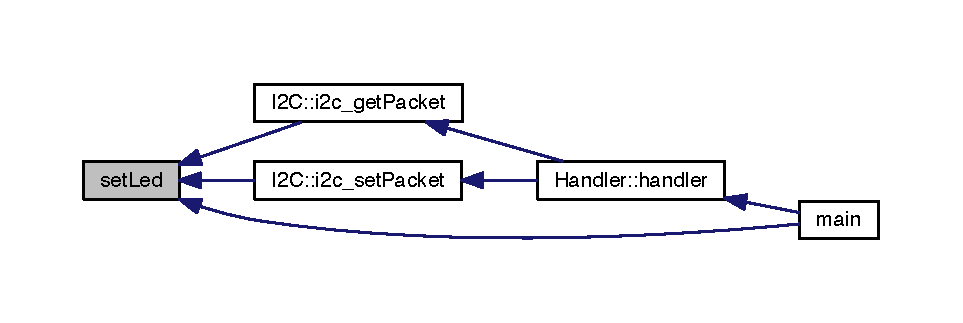
\includegraphics[width=350pt]{d3/dbe/class_l_e_d_a1d8e725e3829da99c1d027ba0a2ce57a_icgraph}
\end{center}
\end{figure}




Dokumentationen for denne klasse blev genereret ud fra filerne\+:\begin{DoxyCompactItemize}
\item 
\hyperlink{led_8h}{led.\+h}\item 
\hyperlink{led_8c}{led.\+c}\end{DoxyCompactItemize}

\hypertarget{class_queue}{}\subsection{Queue Klasse-\/reference}
\label{class_queue}\index{Queue@{Queue}}


\hyperlink{class_queue}{Queue} class.  




{\ttfamily \#include $<$queue.\+h$>$}



Samarbejdsdiagram for Queue\+:
\nopagebreak
\begin{figure}[H]
\begin{center}
\leavevmode
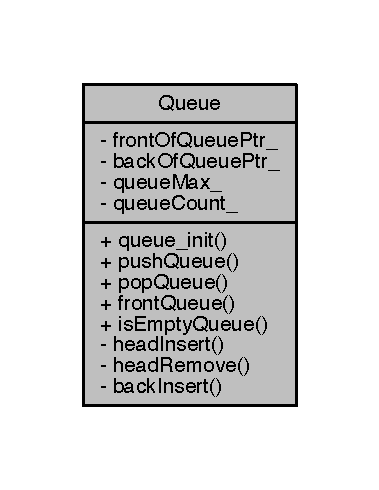
\includegraphics[width=182pt]{d9/d28/class_queue__coll__graph}
\end{center}
\end{figure}
\subsubsection*{Offentlige metoder}
\begin{DoxyCompactItemize}
\item 
void \hyperlink{class_queue_a4e0a3758d721506e7729f4d074a280ff}{queue\+\_\+init} (uint8 queue\+Max\+Size)
\begin{DoxyCompactList}\small\item\em Initialiser \hyperlink{class_queue}{Queue} modulet. \end{DoxyCompactList}\item 
void \hyperlink{class_queue_a0012fa831aa1529e5ed3a6610b733423}{push\+Queue} (const struct \hyperlink{queue_8h_df/d8c/struct_action}{Action} data)
\begin{DoxyCompactList}\small\item\em Indsætter et element i køen. \end{DoxyCompactList}\item 
void \hyperlink{class_queue_a9ecab9ecdedfc331aed9a0ae63ce193b}{pop\+Queue} ()
\begin{DoxyCompactList}\small\item\em Fjerner et element i køen. \end{DoxyCompactList}\item 
struct \hyperlink{queue_8h_df/d8c/struct_action}{Action} \hyperlink{class_queue_a49c50ba30a42033068d8d8e6a23c6ca1}{front\+Queue} ()
\begin{DoxyCompactList}\small\item\em Viser et element fra køen. \end{DoxyCompactList}\item 
uint8 \hyperlink{class_queue_aafb324c79731abdc228dbf94d86722a3}{is\+Empty\+Queue} ()
\begin{DoxyCompactList}\small\item\em Retuner status af køen. \end{DoxyCompactList}\end{DoxyCompactItemize}
\subsubsection*{Private metoder}
\begin{DoxyCompactItemize}
\item 
void \hyperlink{class_queue_a1189c09234d75518492525645a05db07}{head\+Insert} (struct \hyperlink{queue_8c_db/d8b/struct_node}{Node} $\ast$$\ast$head\+Ptr, const struct \hyperlink{queue_8h_df/d8c/struct_action}{Action} data)
\begin{DoxyCompactList}\small\item\em Indsætter forreste i listen. \end{DoxyCompactList}\item 
void \hyperlink{class_queue_ae54666c891fd21d5497f48c385a00b74}{head\+Remove} (struct \hyperlink{queue_8c_db/d8b/struct_node}{Node} $\ast$$\ast$head\+Ptr)
\begin{DoxyCompactList}\small\item\em Fjerner fra listen. \end{DoxyCompactList}\item 
void \hyperlink{class_queue_a5a25a737ba7dff74923f5cb04e19164c}{back\+Insert} (struct \hyperlink{queue_8c_db/d8b/struct_node}{Node} $\ast$$\ast$back\+Ptr, const struct \hyperlink{queue_8h_df/d8c/struct_action}{Action} data)
\begin{DoxyCompactList}\small\item\em Indsætter bagerst i listen. \end{DoxyCompactList}\end{DoxyCompactItemize}
\subsubsection*{Statiske, private attributter}
\begin{DoxyCompactItemize}
\item 
static struct \hyperlink{queue_8c_db/d8b/struct_node}{Node} $\ast$ \hyperlink{class_queue_aa48f05218d0a78402821c8aa9bdad06a}{front\+Of\+Queue\+Ptr\+\_\+}
\begin{DoxyCompactList}\small\item\em Pointer til foreste element i køen. \end{DoxyCompactList}\item 
static struct \hyperlink{queue_8c_db/d8b/struct_node}{Node} $\ast$ \hyperlink{class_queue_a225d2c9ad4e83d6da443e99b8869a51c}{back\+Of\+Queue\+Ptr\+\_\+}
\begin{DoxyCompactList}\small\item\em Pointer til bagerste element i køen. \end{DoxyCompactList}\item 
static uint8 \hyperlink{class_queue_acb6b6e88c9e4d12839594b31e6ff7c5a}{queue\+Max\+\_\+}
\begin{DoxyCompactList}\small\item\em Køens max. \end{DoxyCompactList}\item 
static uint8 \hyperlink{class_queue_ad260f9ccca00e80d161bbf3e70c3ffa6}{queue\+Count\+\_\+}
\begin{DoxyCompactList}\small\item\em Kø element tæller. \end{DoxyCompactList}\end{DoxyCompactItemize}


\subsubsection{Detaljeret beskrivelse}
\hyperlink{class_queue}{Queue} class. 

En F\+I\+FO kø der er opbygget af en single linket liste. \begin{DoxyAuthor}{Forfatter}
Jeppe Stærk Antonsen (\href{mailto:201271201@uni.au.dk}{\tt 201271201@uni.\+au.\+dk}) 
\end{DoxyAuthor}


\subsubsection{Dokumentation af medlemsfunktioner}
\index{Queue@{Queue}!back\+Insert@{back\+Insert}}
\index{back\+Insert@{back\+Insert}!Queue@{Queue}}
\paragraph[{\texorpdfstring{back\+Insert(struct Node $\ast$$\ast$back\+Ptr, const struct Action data)}{backInsert(struct Node **backPtr, const struct Action data)}}]{\setlength{\rightskip}{0pt plus 5cm}void back\+Insert (
\begin{DoxyParamCaption}
\item[{struct {\bf Node} $\ast$$\ast$}]{back\+Ptr, }
\item[{const struct {\bf Action}}]{data}
\end{DoxyParamCaption}
)\hspace{0.3cm}{\ttfamily [private]}}\hypertarget{class_queue_a5a25a737ba7dff74923f5cb04e19164c}{}\label{class_queue_a5a25a737ba7dff74923f5cb04e19164c}


Indsætter bagerst i listen. 

Indsætter det angivet element bagerst i den underlægende linked liste. 
\begin{DoxyParams}[1]{Parametre}
\mbox{\tt in}  & {\em back\+Ptr} & Pointer til det bagerste element i listen. \\
\hline
\mbox{\tt in}  & {\em data} & \hyperlink{class_data}{Data} der skal indsættes i listen.\\
\hline
\end{DoxyParams}
\begin{DoxyAuthor}{Forfatter}
Jeppe Stærk Antonsen (\href{mailto:201271201@uni.au.dk}{\tt 201271201@uni.\+au.\+dk}) 
\end{DoxyAuthor}


Defineret på linje 248 i filen queue.\+c.



Indeholder referencer til Node\+::data\+\_\+ og Node\+::next\+\_\+.


\begin{DoxyCode}
249 \{
250   \textcolor{keywordflow}{if}(*backPtr == NULL)
251   \{
252     \textcolor{keywordflow}{return};
253   \}
254   
255   \textcolor{keyword}{struct }\hyperlink{queue_8c_db/d8b/struct_node}{Node}* next = (*backPtr)->\hyperlink{queue_8c_a882bca6dea645e11ca1df6bc3c30ac42}{next\_};
256   \textcolor{keyword}{struct }\hyperlink{queue_8c_db/d8b/struct_node}{Node}* temp = (\textcolor{keyword}{struct }\hyperlink{queue_8c_db/d8b/struct_node}{Node}*)malloc(\textcolor{keyword}{sizeof}(\textcolor{keyword}{struct} \hyperlink{queue_8c_db/d8b/struct_node}{Node}));
257   temp->\hyperlink{queue_8c_ab134027ce40d71eaa8746f6a8e7d4b8a}{data\_} = data;
258   temp->\hyperlink{queue_8c_a882bca6dea645e11ca1df6bc3c30ac42}{next\_} = next;
259   (*backPtr)->\hyperlink{queue_8c_a882bca6dea645e11ca1df6bc3c30ac42}{next\_} = temp;
260 \}
\end{DoxyCode}
\index{Queue@{Queue}!front\+Queue@{front\+Queue}}
\index{front\+Queue@{front\+Queue}!Queue@{Queue}}
\paragraph[{\texorpdfstring{front\+Queue()}{frontQueue()}}]{\setlength{\rightskip}{0pt plus 5cm}struct {\bf Action} front\+Queue (
\begin{DoxyParamCaption}
\item[{void}]{}
\end{DoxyParamCaption}
)}\hypertarget{class_queue_a49c50ba30a42033068d8d8e6a23c6ca1}{}\label{class_queue_a49c50ba30a42033068d8d8e6a23c6ca1}


Viser et element fra køen. 

Viser det foreste element i F\+I\+FO køen.

\begin{DoxyAuthor}{Forfatter}
Jeppe Stærk Antonsen (\href{mailto:201271201@uni.au.dk}{\tt 201271201@uni.\+au.\+dk}) 
\end{DoxyAuthor}


Defineret på linje 170 i filen queue.\+c.



Indeholder referencer til Node\+::data\+\_\+.



Refereret til af main().


\begin{DoxyCode}
171 \{
172   DEBUG\_PutString(\textcolor{stringliteral}{"Q=: count: "});
173   DEBUG\_PutHexByte(\hyperlink{class_queue_ad260f9ccca00e80d161bbf3e70c3ffa6}{queueCount\_});
174   DEBUG\_PutCRLF();
175   \textcolor{keywordflow}{return} \hyperlink{class_queue_aa48f05218d0a78402821c8aa9bdad06a}{frontOfQueuePtr\_}->\hyperlink{queue_8c_ab134027ce40d71eaa8746f6a8e7d4b8a}{data\_};
176 \}
\end{DoxyCode}


Her er kalder-\/grafen for denne funktion\+:
\nopagebreak
\begin{figure}[H]
\begin{center}
\leavevmode
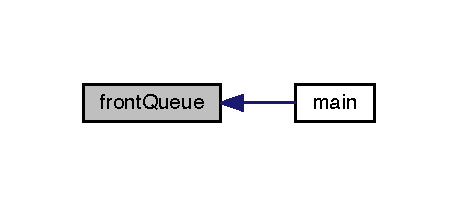
\includegraphics[width=220pt]{d4/da4/class_queue_a49c50ba30a42033068d8d8e6a23c6ca1_icgraph}
\end{center}
\end{figure}


\index{Queue@{Queue}!head\+Insert@{head\+Insert}}
\index{head\+Insert@{head\+Insert}!Queue@{Queue}}
\paragraph[{\texorpdfstring{head\+Insert(struct Node $\ast$$\ast$head\+Ptr, const struct Action data)}{headInsert(struct Node **headPtr, const struct Action data)}}]{\setlength{\rightskip}{0pt plus 5cm}void head\+Insert (
\begin{DoxyParamCaption}
\item[{struct {\bf Node} $\ast$$\ast$}]{head\+Ptr, }
\item[{const struct {\bf Action}}]{data}
\end{DoxyParamCaption}
)\hspace{0.3cm}{\ttfamily [private]}}\hypertarget{class_queue_a1189c09234d75518492525645a05db07}{}\label{class_queue_a1189c09234d75518492525645a05db07}


Indsætter forreste i listen. 

Indsætter det angivet element forreste i den underlægende linked liste. 
\begin{DoxyParams}[1]{Parametre}
\mbox{\tt in}  & {\em head\+Ptr} & Pointer til det foreste element i listen. \\
\hline
\mbox{\tt in}  & {\em data} & \hyperlink{class_data}{Data} der skal indsættes i listen.\\
\hline
\end{DoxyParams}
\begin{DoxyAuthor}{Forfatter}
Jeppe Stærk Antonsen (\href{mailto:201271201@uni.au.dk}{\tt 201271201@uni.\+au.\+dk}) 
\end{DoxyAuthor}


Defineret på linje 206 i filen queue.\+c.



Indeholder referencer til Node\+::data\+\_\+ og Node\+::next\+\_\+.


\begin{DoxyCode}
207 \{
208   \textcolor{keyword}{struct }\hyperlink{queue_8c_db/d8b/struct_node}{Node}* temp = (\textcolor{keyword}{struct }\hyperlink{queue_8c_db/d8b/struct_node}{Node}*)malloc(\textcolor{keyword}{sizeof}(\textcolor{keyword}{struct} \hyperlink{queue_8c_db/d8b/struct_node}{Node}));
209   \textcolor{keywordflow}{if}(temp == NULL)
210   \{
211     \textcolor{keywordflow}{return};
212   \}
213   
214   temp->\hyperlink{queue_8c_ab134027ce40d71eaa8746f6a8e7d4b8a}{data\_} = data;
215   temp->\hyperlink{queue_8c_a882bca6dea645e11ca1df6bc3c30ac42}{next\_} = NULL;
216   
217   *headPtr = temp;
218 \}
\end{DoxyCode}
\index{Queue@{Queue}!head\+Remove@{head\+Remove}}
\index{head\+Remove@{head\+Remove}!Queue@{Queue}}
\paragraph[{\texorpdfstring{head\+Remove(struct Node $\ast$$\ast$head\+Ptr)}{headRemove(struct Node **headPtr)}}]{\setlength{\rightskip}{0pt plus 5cm}void head\+Remove (
\begin{DoxyParamCaption}
\item[{struct {\bf Node} $\ast$$\ast$}]{head\+Ptr}
\end{DoxyParamCaption}
)\hspace{0.3cm}{\ttfamily [private]}}\hypertarget{class_queue_ae54666c891fd21d5497f48c385a00b74}{}\label{class_queue_ae54666c891fd21d5497f48c385a00b74}


Fjerner fra listen. 

Fjerner det forreste element i den underlæggende linked liste 
\begin{DoxyParams}[1]{Parametre}
\mbox{\tt in}  & {\em head\+Ptr} & Pointer til det forreste element i listen.\\
\hline
\end{DoxyParams}
\begin{DoxyAuthor}{Forfatter}
Jeppe Stærk Antonsen (\href{mailto:201271201@uni.au.dk}{\tt 201271201@uni.\+au.\+dk}) 
\end{DoxyAuthor}


Defineret på linje 228 i filen queue.\+c.



Indeholder referencer til Node\+::next\+\_\+.


\begin{DoxyCode}
229 \{
230   \textcolor{keywordflow}{if}(headPtr != NULL)
231   \{
232     \textcolor{keyword}{struct }\hyperlink{queue_8c_db/d8b/struct_node}{Node}* condemned;
233     condemned = *headPtr;
234     *headPtr = (*headPtr)->\hyperlink{queue_8c_a882bca6dea645e11ca1df6bc3c30ac42}{next\_};
235     free(condemned);
236   \}
237 \}
\end{DoxyCode}
\index{Queue@{Queue}!is\+Empty\+Queue@{is\+Empty\+Queue}}
\index{is\+Empty\+Queue@{is\+Empty\+Queue}!Queue@{Queue}}
\paragraph[{\texorpdfstring{is\+Empty\+Queue()}{isEmptyQueue()}}]{\setlength{\rightskip}{0pt plus 5cm}uint8 is\+Empty\+Queue (
\begin{DoxyParamCaption}
\item[{void}]{}
\end{DoxyParamCaption}
)}\hypertarget{class_queue_aafb324c79731abdc228dbf94d86722a3}{}\label{class_queue_aafb324c79731abdc228dbf94d86722a3}


Retuner status af køen. 

Kontrollere om køen er tom.

\begin{DoxyAuthor}{Forfatter}
Jeppe Stærk Antonsen (\href{mailto:201271201@uni.au.dk}{\tt 201271201@uni.\+au.\+dk}) 
\end{DoxyAuthor}


Defineret på linje 185 i filen queue.\+c.



Refereret til af main().


\begin{DoxyCode}
186 \{
187   \textcolor{keywordflow}{if}(\hyperlink{class_queue_aa48f05218d0a78402821c8aa9bdad06a}{frontOfQueuePtr\_} == NULL)
188   \{
189     \textcolor{keywordflow}{return} 1;
190   \}
191   \textcolor{keywordflow}{else}
192   \{
193     \textcolor{keywordflow}{return} 0;
194   \}
195 \}
\end{DoxyCode}


Her er kalder-\/grafen for denne funktion\+:
\nopagebreak
\begin{figure}[H]
\begin{center}
\leavevmode
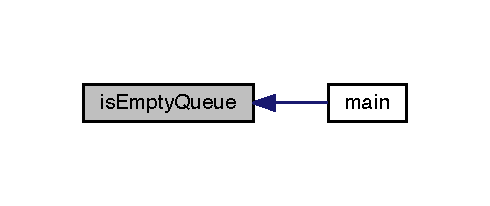
\includegraphics[width=235pt]{d4/da4/class_queue_aafb324c79731abdc228dbf94d86722a3_icgraph}
\end{center}
\end{figure}


\index{Queue@{Queue}!pop\+Queue@{pop\+Queue}}
\index{pop\+Queue@{pop\+Queue}!Queue@{Queue}}
\paragraph[{\texorpdfstring{pop\+Queue()}{popQueue()}}]{\setlength{\rightskip}{0pt plus 5cm}void pop\+Queue (
\begin{DoxyParamCaption}
\item[{void}]{}
\end{DoxyParamCaption}
)}\hypertarget{class_queue_a9ecab9ecdedfc331aed9a0ae63ce193b}{}\label{class_queue_a9ecab9ecdedfc331aed9a0ae63ce193b}


Fjerner et element i køen. 

Fjerner det foreste element i F\+I\+FO køen.

\begin{DoxyAuthor}{Forfatter}
Jeppe Stærk Antonsen (\href{mailto:201271201@uni.au.dk}{\tt 201271201@uni.\+au.\+dk}) 
\end{DoxyAuthor}


Defineret på linje 149 i filen queue.\+c.



Indeholder referencer til head\+Remove() og is\+Empty\+Queue().



Refereret til af main().


\begin{DoxyCode}
150 \{
151   \hyperlink{class_queue_ae54666c891fd21d5497f48c385a00b74}{headRemove}(&\hyperlink{class_queue_aa48f05218d0a78402821c8aa9bdad06a}{frontOfQueuePtr\_});
152   \hyperlink{class_queue_ad260f9ccca00e80d161bbf3e70c3ffa6}{queueCount\_}--;
153   \textcolor{keywordflow}{if}(\hyperlink{class_queue_aafb324c79731abdc228dbf94d86722a3}{isEmptyQueue}() == 1)
154   \{
155     \hyperlink{class_queue_a225d2c9ad4e83d6da443e99b8869a51c}{backOfQueuePtr\_} = NULL;
156   \}
157   DEBUG\_PutString(\textcolor{stringliteral}{"-Q: count: "});
158   DEBUG\_PutHexByte(\hyperlink{class_queue_ad260f9ccca00e80d161bbf3e70c3ffa6}{queueCount\_});
159   DEBUG\_PutCRLF();
160   DEBUG\_PutCRLF();
161 \}
\end{DoxyCode}


Her er kald-\/grafen for denne funktion\+:
\nopagebreak
\begin{figure}[H]
\begin{center}
\leavevmode
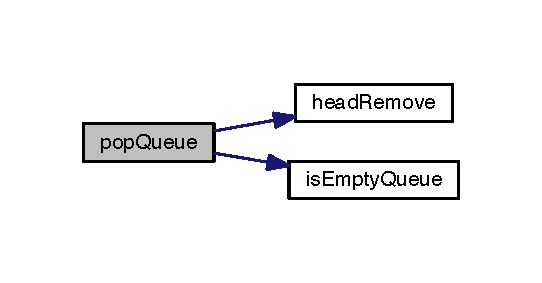
\includegraphics[width=260pt]{d4/da4/class_queue_a9ecab9ecdedfc331aed9a0ae63ce193b_cgraph}
\end{center}
\end{figure}




Her er kalder-\/grafen for denne funktion\+:
\nopagebreak
\begin{figure}[H]
\begin{center}
\leavevmode
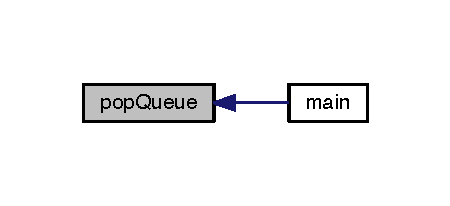
\includegraphics[width=216pt]{d4/da4/class_queue_a9ecab9ecdedfc331aed9a0ae63ce193b_icgraph}
\end{center}
\end{figure}


\index{Queue@{Queue}!push\+Queue@{push\+Queue}}
\index{push\+Queue@{push\+Queue}!Queue@{Queue}}
\paragraph[{\texorpdfstring{push\+Queue(const struct Action data)}{pushQueue(const struct Action data)}}]{\setlength{\rightskip}{0pt plus 5cm}void push\+Queue (
\begin{DoxyParamCaption}
\item[{const struct {\bf Action}}]{data}
\end{DoxyParamCaption}
)}\hypertarget{class_queue_a0012fa831aa1529e5ed3a6610b733423}{}\label{class_queue_a0012fa831aa1529e5ed3a6610b733423}


Indsætter et element i køen. 

Indsætter det angivet element bagerst i F\+I\+FO køen. 
\begin{DoxyParams}[1]{Parametre}
\mbox{\tt in}  & {\em data} & \hyperlink{class_data}{Data} der skal indsættes i køen.\\
\hline
\end{DoxyParams}
\begin{DoxyAuthor}{Forfatter}
Jeppe Stærk Antonsen (\href{mailto:201271201@uni.au.dk}{\tt 201271201@uni.\+au.\+dk}) 
\end{DoxyAuthor}


Defineret på linje 107 i filen queue.\+c.



Indeholder referencer til back\+Insert(), Action\+::cmd, head\+Insert(), is\+Empty\+Queue(), Node\+::next\+\_\+ og Action\+::val.



Refereret til af I2\+C\+::\+I2\+C\+S\+\_\+\+I2\+C\+\_\+\+I\+S\+R\+\_\+\+Exit\+Callback().


\begin{DoxyCode}
108 \{
109   \textcolor{keywordflow}{if}(\hyperlink{class_queue_ad260f9ccca00e80d161bbf3e70c3ffa6}{queueCount\_}<\hyperlink{class_queue_acb6b6e88c9e4d12839594b31e6ff7c5a}{queueMax\_})
110   \{
111     \textcolor{keywordflow}{if}(\hyperlink{class_queue_aafb324c79731abdc228dbf94d86722a3}{isEmptyQueue}() != 1)
112     \{
113       \hyperlink{class_queue_a5a25a737ba7dff74923f5cb04e19164c}{backInsert}(&\hyperlink{class_queue_a225d2c9ad4e83d6da443e99b8869a51c}{backOfQueuePtr\_}, data);
114       \hyperlink{class_queue_a225d2c9ad4e83d6da443e99b8869a51c}{backOfQueuePtr\_} = \hyperlink{class_queue_a225d2c9ad4e83d6da443e99b8869a51c}{backOfQueuePtr\_}->\hyperlink{queue_8c_a882bca6dea645e11ca1df6bc3c30ac42}{next\_};
115       \hyperlink{class_queue_ad260f9ccca00e80d161bbf3e70c3ffa6}{queueCount\_}++;
116     \}
117     \textcolor{keywordflow}{else}
118     \{
119       \hyperlink{class_queue_a1189c09234d75518492525645a05db07}{headInsert}(&\hyperlink{class_queue_aa48f05218d0a78402821c8aa9bdad06a}{frontOfQueuePtr\_}, data);
120       \hyperlink{class_queue_a225d2c9ad4e83d6da443e99b8869a51c}{backOfQueuePtr\_} = \hyperlink{class_queue_aa48f05218d0a78402821c8aa9bdad06a}{frontOfQueuePtr\_};
121       \hyperlink{class_queue_ad260f9ccca00e80d161bbf3e70c3ffa6}{queueCount\_}++;
122     \}
123     DEBUG\_PutString(\textcolor{stringliteral}{"Q+: count: "});
124     DEBUG\_PutHexByte(\hyperlink{class_queue_ad260f9ccca00e80d161bbf3e70c3ffa6}{queueCount\_});
125     DEBUG\_PutString(\textcolor{stringliteral}{" cmd: "});
126     DEBUG\_PutHexByte(data.\hyperlink{queue_8h_a85092d82ab6ea85dad51ba78cbda36a0}{cmd});
127     DEBUG\_PutString(\textcolor{stringliteral}{" val: "});
128     DEBUG\_PutHexByte(data.\hyperlink{queue_8h_aa0ccb5ee6d882ee3605ff47745c6467b}{val});
129     DEBUG\_PutCRLF();
130     DEBUG\_PutCRLF();
131   \}
132   \textcolor{keywordflow}{else}
133   \{
134     DEBUG\_PutString(\textcolor{stringliteral}{"Q~: ERROR! Queue FULL!!! count: "});
135     DEBUG\_PutHexByte(\hyperlink{class_queue_ad260f9ccca00e80d161bbf3e70c3ffa6}{queueCount\_});
136     DEBUG\_PutCRLF();
137     DEBUG\_PutCRLF();
138   \}
139   
140 \}
\end{DoxyCode}


Her er kald-\/grafen for denne funktion\+:
\nopagebreak
\begin{figure}[H]
\begin{center}
\leavevmode
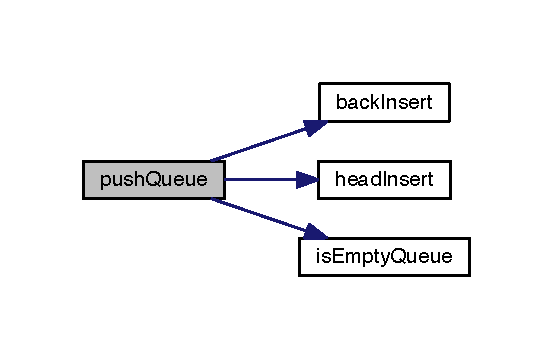
\includegraphics[width=265pt]{d4/da4/class_queue_a0012fa831aa1529e5ed3a6610b733423_cgraph}
\end{center}
\end{figure}




Her er kalder-\/grafen for denne funktion\+:
\nopagebreak
\begin{figure}[H]
\begin{center}
\leavevmode
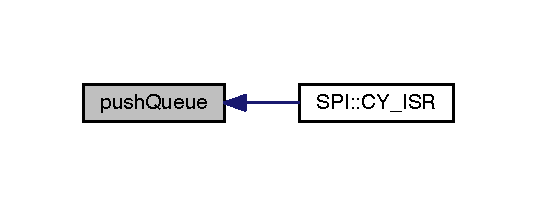
\includegraphics[width=347pt]{d4/da4/class_queue_a0012fa831aa1529e5ed3a6610b733423_icgraph}
\end{center}
\end{figure}


\index{Queue@{Queue}!queue\+\_\+init@{queue\+\_\+init}}
\index{queue\+\_\+init@{queue\+\_\+init}!Queue@{Queue}}
\paragraph[{\texorpdfstring{queue\+\_\+init(uint8 queue\+Max\+Size)}{queue_init(uint8 queueMaxSize)}}]{\setlength{\rightskip}{0pt plus 5cm}void queue\+\_\+init (
\begin{DoxyParamCaption}
\item[{uint8}]{queue\+Max\+Size}
\end{DoxyParamCaption}
)}\hypertarget{class_queue_a4e0a3758d721506e7729f4d074a280ff}{}\label{class_queue_a4e0a3758d721506e7729f4d074a280ff}


Initialiser \hyperlink{class_queue}{Queue} modulet. 

Initailiser køen med den ønsket max størelse.

\begin{DoxyAuthor}{Forfatter}
Jeppe Stærk Antonsen (\href{mailto:201271201@uni.au.dk}{\tt 201271201@uni.\+au.\+dk}) 
\end{DoxyAuthor}


Defineret på linje 89 i filen queue.\+c.



Indeholder referencer til Node\+::next\+\_\+.



Refereret til af main().


\begin{DoxyCode}
90 \{
91   \hyperlink{class_queue_aa48f05218d0a78402821c8aa9bdad06a}{frontOfQueuePtr\_} = NULL;
92   \hyperlink{class_queue_aa48f05218d0a78402821c8aa9bdad06a}{frontOfQueuePtr\_}->\hyperlink{queue_8c_a882bca6dea645e11ca1df6bc3c30ac42}{next\_} = NULL;
93   \hyperlink{class_queue_a225d2c9ad4e83d6da443e99b8869a51c}{backOfQueuePtr\_} = NULL;
94   \hyperlink{class_queue_a225d2c9ad4e83d6da443e99b8869a51c}{backOfQueuePtr\_}->\hyperlink{queue_8c_a882bca6dea645e11ca1df6bc3c30ac42}{next\_} = NULL;
95   \hyperlink{class_queue_acb6b6e88c9e4d12839594b31e6ff7c5a}{queueMax\_} = queueMaxSize;
96   \hyperlink{class_queue_ad260f9ccca00e80d161bbf3e70c3ffa6}{queueCount\_} = 0;
97 \}
\end{DoxyCode}


Her er kalder-\/grafen for denne funktion\+:
\nopagebreak
\begin{figure}[H]
\begin{center}
\leavevmode
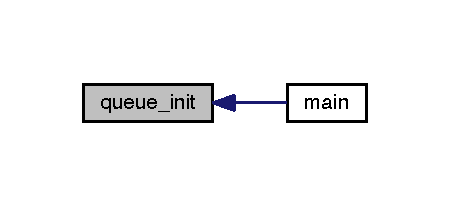
\includegraphics[width=216pt]{d4/da4/class_queue_a4e0a3758d721506e7729f4d074a280ff_icgraph}
\end{center}
\end{figure}




\subsubsection{Felt-\/dokumentation}
\index{Queue@{Queue}!back\+Of\+Queue\+Ptr\+\_\+@{back\+Of\+Queue\+Ptr\+\_\+}}
\index{back\+Of\+Queue\+Ptr\+\_\+@{back\+Of\+Queue\+Ptr\+\_\+}!Queue@{Queue}}
\paragraph[{\texorpdfstring{back\+Of\+Queue\+Ptr\+\_\+}{backOfQueuePtr_}}]{\setlength{\rightskip}{0pt plus 5cm}struct {\bf Node}$\ast$ back\+Of\+Queue\+Ptr\+\_\+\hspace{0.3cm}{\ttfamily [static]}, {\ttfamily [private]}}\hypertarget{class_queue_a225d2c9ad4e83d6da443e99b8869a51c}{}\label{class_queue_a225d2c9ad4e83d6da443e99b8869a51c}


Pointer til bagerste element i køen. 

En \hyperlink{queue_8c_db/d8b/struct_node}{Node} pointer der indeholder adressen på det bagerste elementet i køen.

\begin{DoxyAuthor}{Forfatter}
Jeppe Stærk Antonsen (\href{mailto:201271201@uni.au.dk}{\tt 201271201@uni.\+au.\+dk}) 
\end{DoxyAuthor}


Defineret på linje 48 i filen queue.\+c.

\index{Queue@{Queue}!front\+Of\+Queue\+Ptr\+\_\+@{front\+Of\+Queue\+Ptr\+\_\+}}
\index{front\+Of\+Queue\+Ptr\+\_\+@{front\+Of\+Queue\+Ptr\+\_\+}!Queue@{Queue}}
\paragraph[{\texorpdfstring{front\+Of\+Queue\+Ptr\+\_\+}{frontOfQueuePtr_}}]{\setlength{\rightskip}{0pt plus 5cm}struct {\bf Node}$\ast$ front\+Of\+Queue\+Ptr\+\_\+\hspace{0.3cm}{\ttfamily [static]}, {\ttfamily [private]}}\hypertarget{class_queue_aa48f05218d0a78402821c8aa9bdad06a}{}\label{class_queue_aa48f05218d0a78402821c8aa9bdad06a}


Pointer til foreste element i køen. 

En \hyperlink{queue_8c_db/d8b/struct_node}{Node} pointer der indeholder adressen på det foreste elementet i køen.

\begin{DoxyAuthor}{Forfatter}
Jeppe Stærk Antonsen (\href{mailto:201271201@uni.au.dk}{\tt 201271201@uni.\+au.\+dk}) 
\end{DoxyAuthor}


Defineret på linje 39 i filen queue.\+c.

\index{Queue@{Queue}!queue\+Count\+\_\+@{queue\+Count\+\_\+}}
\index{queue\+Count\+\_\+@{queue\+Count\+\_\+}!Queue@{Queue}}
\paragraph[{\texorpdfstring{queue\+Count\+\_\+}{queueCount_}}]{\setlength{\rightskip}{0pt plus 5cm}uint8 queue\+Count\+\_\+\hspace{0.3cm}{\ttfamily [static]}, {\ttfamily [private]}}\hypertarget{class_queue_ad260f9ccca00e80d161bbf3e70c3ffa6}{}\label{class_queue_ad260f9ccca00e80d161bbf3e70c3ffa6}


Kø element tæller. 

Bruges til at tælle hvor mange elementer der er i køen.

\begin{DoxyAuthor}{Forfatter}
Jeppe Stærk Antonsen (\href{mailto:201271201@uni.au.dk}{\tt 201271201@uni.\+au.\+dk}) 
\end{DoxyAuthor}


Defineret på linje 66 i filen queue.\+c.

\index{Queue@{Queue}!queue\+Max\+\_\+@{queue\+Max\+\_\+}}
\index{queue\+Max\+\_\+@{queue\+Max\+\_\+}!Queue@{Queue}}
\paragraph[{\texorpdfstring{queue\+Max\+\_\+}{queueMax_}}]{\setlength{\rightskip}{0pt plus 5cm}uint8 queue\+Max\+\_\+\hspace{0.3cm}{\ttfamily [static]}, {\ttfamily [private]}}\hypertarget{class_queue_acb6b6e88c9e4d12839594b31e6ff7c5a}{}\label{class_queue_acb6b6e88c9e4d12839594b31e6ff7c5a}


Køens max. 

Laver ved initialisering der ønsket antal for max elementer i køen

\begin{DoxyAuthor}{Forfatter}
Jeppe Stærk Antonsen (\href{mailto:201271201@uni.au.dk}{\tt 201271201@uni.\+au.\+dk}) 
\end{DoxyAuthor}


Defineret på linje 57 i filen queue.\+c.



Dokumentationen for denne klasse blev genereret ud fra filerne\+:\begin{DoxyCompactItemize}
\item 
\hyperlink{queue_8h}{queue.\+h}\item 
\hyperlink{queue_8c}{queue.\+c}\end{DoxyCompactItemize}

\hypertarget{class_s_p_i}{}\subsection{S\+PI Klasse-\/reference}
\label{class_s_p_i}\index{S\+PI@{S\+PI}}


\hyperlink{class_s_p_i}{S\+PI} class.  




{\ttfamily \#include $<$spi.\+h$>$}



Samarbejdsdiagram for S\+PI\+:\nopagebreak
\begin{figure}[H]
\begin{center}
\leavevmode
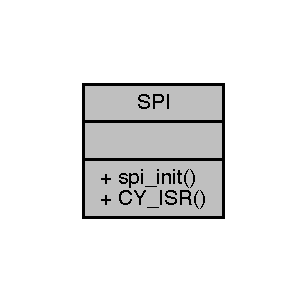
\includegraphics[width=147pt]{dd/d16/class_s_p_i__coll__graph}
\end{center}
\end{figure}
\subsubsection*{Offentlige metoder}
\begin{DoxyCompactItemize}
\item 
void \hyperlink{class_s_p_i_a5db0aceecaf7db5fbe2984e88fef3734}{spi\+\_\+init} ()
\begin{DoxyCompactList}\small\item\em Initialiser \hyperlink{class_s_p_i}{S\+PI} modulet. \end{DoxyCompactList}\item 
\hyperlink{class_s_p_i_ae65228150b9bf9ec06e2c3260dcbc328}{C\+Y\+\_\+\+I\+SR} (isr\+\_\+spi\+\_\+rx)
\begin{DoxyCompactList}\small\item\em Modtager kald fra S\+P\+I-\/busset. \end{DoxyCompactList}\end{DoxyCompactItemize}


\subsubsection{Detaljeret beskrivelse}
\hyperlink{class_s_p_i}{S\+PI} class. 

Håndter kommunikation via S\+P\+I-\/busset. \begin{DoxyAuthor}{Forfatter}
Jeppe Stærk Antonsen (\href{mailto:201271201@uni.au.dk}{\tt 201271201@uni.\+au.\+dk}) 
\end{DoxyAuthor}


\subsubsection{Dokumentation af medlemsfunktioner}
\index{S\+PI@{S\+PI}!C\+Y\+\_\+\+I\+SR@{C\+Y\+\_\+\+I\+SR}}
\index{C\+Y\+\_\+\+I\+SR@{C\+Y\+\_\+\+I\+SR}!S\+PI@{S\+PI}}
\paragraph[{\texorpdfstring{C\+Y\+\_\+\+I\+S\+R(isr\+\_\+spi\+\_\+rx)}{CY_ISR(isr_spi_rx)}}]{\setlength{\rightskip}{0pt plus 5cm}C\+Y\+\_\+\+I\+SR (
\begin{DoxyParamCaption}
\item[{isr\+\_\+spi\+\_\+rx}]{}
\end{DoxyParamCaption}
)}\hypertarget{class_s_p_i_ae65228150b9bf9ec06e2c3260dcbc328}{}\label{class_s_p_i_ae65228150b9bf9ec06e2c3260dcbc328}


Modtager kald fra S\+P\+I-\/busset. 

En \char`\"{}\+Interrupt Service Routine(\+I\+S\+R)\char`\"{} der aktiveres ved modtagelse af kald via S\+P\+I-\/busset, det modtaget data behandles og håndteres.

\begin{DoxyAuthor}{Forfatter}
Jeppe Stærk (\href{mailto:201271201@uni.au.dk}{\tt 201271201@uni.\+au.\+dk}) 
\end{DoxyAuthor}


Defineret på linje 41 i filen spi.\+c.



Indeholder referencer til Data\+Master\+::b\+Val, Action\+::cmd, C\+M\+D\+\_\+\+G\+E\+T\+\_\+\+B\+L\+U\+E\+\_\+\+V\+AL, C\+M\+D\+\_\+\+G\+E\+T\+\_\+\+G\+R\+E\+E\+N\+\_\+\+V\+AL, C\+M\+D\+\_\+\+G\+E\+T\+\_\+\+R\+E\+D\+\_\+\+V\+AL, C\+M\+D\+\_\+\+G\+E\+T\+\_\+\+X\+\_\+\+P\+OS, C\+M\+D\+\_\+\+G\+E\+T\+\_\+\+Y\+\_\+\+P\+OS, C\+M\+D\+\_\+\+G\+E\+T\+\_\+\+Z\+\_\+\+P\+OS, data\+Master, Data\+Master\+::g\+Val, L\+C\+D\+::lcd\+\_\+newline(), Queue\+::push\+Queue(), Data\+Master\+::r\+Val, S\+P\+I\+\_\+\+P\+A\+C\+K\+E\+T\+\_\+\+D\+A\+T\+A\+\_\+\+P\+OS, S\+P\+I\+\_\+\+P\+A\+C\+K\+E\+T\+\_\+\+S\+I\+ZE, Action\+::val, Data\+Master\+::x\+Val, Data\+Master\+::y\+Val og Data\+Master\+::z\+Val.


\begin{DoxyCode}
42 \{
43   SPIS\_DisableInt();
44   \textcolor{keywordtype}{char} lcd[12];
45   uint16 spiRxBuffer[\hyperlink{spi_8h_aea54fc09a960e5a1b7096374f3eebee4}{SPI\_PACKET\_SIZE}];
46   uint16 spiTxBuffer[\hyperlink{spi_8h_aea54fc09a960e5a1b7096374f3eebee4}{SPI\_PACKET\_SIZE}];
47   \textcolor{keyword}{struct }\hyperlink{queue_8h_df/d8c/struct_action}{Action} spiRxAction;
48   DEBUG\_PutString(\textcolor{stringliteral}{"SPI!"});
49   DEBUG\_PutCRLF();
50 
51   \textcolor{keywordflow}{while}(SPIS\_SpiUartGetRxBufferSize() > 0)
52   \{
53     spiRxBuffer[\hyperlink{spi_8h_a5ffe58623f478b7b960a1349530a6655}{SPI\_PACKET\_DATA\_POS}] = SPIS\_SpiUartReadRxData();
54     spiRxAction.val = spiRxBuffer[\hyperlink{spi_8h_a5ffe58623f478b7b960a1349530a6655}{SPI\_PACKET\_DATA\_POS}] & 0xff;
55     spiRxAction.cmd = (spiRxBuffer[\hyperlink{spi_8h_a5ffe58623f478b7b960a1349530a6655}{SPI\_PACKET\_DATA\_POS}] >> 8);
56     
57     \textcolor{keywordflow}{if}(spiRxBuffer[\hyperlink{spi_8h_a5ffe58623f478b7b960a1349530a6655}{SPI\_PACKET\_DATA\_POS}] == 0xBADA)
58     \{
59       sprintf(lcd, \textcolor{stringliteral}{"S> %x"},spiTxBuffer[\hyperlink{spi_8h_a5ffe58623f478b7b960a1349530a6655}{SPI\_PACKET\_DATA\_POS}]);
60       \hyperlink{lcd_8h_a507dd352aee8161dc556e3d1439a2be2}{lcd\_newline}(lcd);
61       
62       DEBUG\_PutString(\textcolor{stringliteral}{"S>: val: "});
63       DEBUG\_PutHexByte(spiTxBuffer[\hyperlink{spi_8h_a5ffe58623f478b7b960a1349530a6655}{SPI\_PACKET\_DATA\_POS}]);
64       DEBUG\_PutCRLF();
65     \}
66     \textcolor{keywordflow}{else}
67     \{
68       sprintf(lcd, \textcolor{stringliteral}{">S %4x %2x"}, (\textcolor{keywordtype}{int})spiRxAction.cmd, (\textcolor{keywordtype}{int})spiRxAction.val);
69       \hyperlink{lcd_8h_a507dd352aee8161dc556e3d1439a2be2}{lcd\_newline}(lcd);
70       
71       DEBUG\_PutString(\textcolor{stringliteral}{">S: cmd: "});
72       DEBUG\_PutHexByte(spiRxAction.cmd);
73       DEBUG\_PutString(\textcolor{stringliteral}{" val: "});
74       DEBUG\_PutHexByte(spiRxAction.val);
75       DEBUG\_PutCRLF();
76       DEBUG\_PutCRLF();
77       
78       \textcolor{keywordflow}{switch}(spiRxAction.cmd) \{
79         \textcolor{keywordflow}{case} \hyperlink{handler_8h_aa50e083669624eeaef782ebc867008f9}{CMD\_GET\_X\_POS} :
80           SPIS\_SpiUartClearTxBuffer();
81           spiTxBuffer[\hyperlink{spi_8h_a5ffe58623f478b7b960a1349530a6655}{SPI\_PACKET\_DATA\_POS}] = (uint16)
      \hyperlink{data_8h_a6b1a8871e30b304a6f5764c44d89e489}{dataMaster}.\hyperlink{data_8h_a7849f509240fa25127fcda8c5009f02b}{xVal};
82           SPIS\_SpiUartPutArray(spiTxBuffer, \hyperlink{spi_8h_aea54fc09a960e5a1b7096374f3eebee4}{SPI\_PACKET\_SIZE});
83           \textcolor{keywordflow}{break};
84         \textcolor{keywordflow}{case} \hyperlink{handler_8h_a51053e5251048d6ebbf4d2e23de40761}{CMD\_GET\_Y\_POS} :
85           SPIS\_SpiUartClearTxBuffer();
86           spiTxBuffer[\hyperlink{spi_8h_a5ffe58623f478b7b960a1349530a6655}{SPI\_PACKET\_DATA\_POS}] = (uint16)
      \hyperlink{data_8h_a6b1a8871e30b304a6f5764c44d89e489}{dataMaster}.\hyperlink{data_8h_a28e89368b5a1aee30ccd952ad63e8c55}{yVal};
87           SPIS\_SpiUartPutArray(spiTxBuffer, \hyperlink{spi_8h_aea54fc09a960e5a1b7096374f3eebee4}{SPI\_PACKET\_SIZE});
88           \textcolor{keywordflow}{break};
89         \textcolor{keywordflow}{case} \hyperlink{handler_8h_a4d76e78d09a00f75609569d9aa92ab98}{CMD\_GET\_Z\_POS} :
90           SPIS\_SpiUartClearTxBuffer();
91           spiTxBuffer[\hyperlink{spi_8h_a5ffe58623f478b7b960a1349530a6655}{SPI\_PACKET\_DATA\_POS}] = (uint16)
      \hyperlink{data_8h_a6b1a8871e30b304a6f5764c44d89e489}{dataMaster}.\hyperlink{data_8h_a767a084c35fdc0f1e3e41972d5415483}{zVal};
92           SPIS\_SpiUartPutArray(spiTxBuffer, \hyperlink{spi_8h_aea54fc09a960e5a1b7096374f3eebee4}{SPI\_PACKET\_SIZE});
93           \textcolor{keywordflow}{break};
94         \textcolor{keywordflow}{case} \hyperlink{handler_8h_aa2f09e60c4eeae4560da88c6b1b08c60}{CMD\_GET\_RED\_VAL} :
95           SPIS\_SpiUartClearTxBuffer();
96           spiTxBuffer[\hyperlink{spi_8h_a5ffe58623f478b7b960a1349530a6655}{SPI\_PACKET\_DATA\_POS}] = (uint16)
      \hyperlink{data_8h_a6b1a8871e30b304a6f5764c44d89e489}{dataMaster}.\hyperlink{data_8h_a3bf14030a39e71a91c0b97a624f95c5d}{rVal};
97           SPIS\_SpiUartPutArray(spiTxBuffer, \hyperlink{spi_8h_aea54fc09a960e5a1b7096374f3eebee4}{SPI\_PACKET\_SIZE});
98           \textcolor{keywordflow}{break};
99         \textcolor{keywordflow}{case} \hyperlink{handler_8h_a55d24f50aeb52afddd491d97a66c81ef}{CMD\_GET\_GREEN\_VAL} :
100           SPIS\_SpiUartClearTxBuffer();
101           spiTxBuffer[\hyperlink{spi_8h_a5ffe58623f478b7b960a1349530a6655}{SPI\_PACKET\_DATA\_POS}] = (uint16)
      \hyperlink{data_8h_a6b1a8871e30b304a6f5764c44d89e489}{dataMaster}.\hyperlink{data_8h_ae02d0c792549f1b88e80ae6eb117f2be}{gVal};
102           SPIS\_SpiUartPutArray(spiTxBuffer, \hyperlink{spi_8h_aea54fc09a960e5a1b7096374f3eebee4}{SPI\_PACKET\_SIZE});
103           \textcolor{keywordflow}{break};
104         \textcolor{keywordflow}{case} \hyperlink{handler_8h_a81052c67f996705d7eacfcea66bdde08}{CMD\_GET\_BLUE\_VAL} :
105           SPIS\_SpiUartClearTxBuffer();
106           spiTxBuffer[\hyperlink{spi_8h_a5ffe58623f478b7b960a1349530a6655}{SPI\_PACKET\_DATA\_POS}] = (uint16)
      \hyperlink{data_8h_a6b1a8871e30b304a6f5764c44d89e489}{dataMaster}.\hyperlink{data_8h_adf9e1f80891d4eaa914c2bde2502cdf2}{bVal};
107           SPIS\_SpiUartPutArray(spiTxBuffer, \hyperlink{spi_8h_aea54fc09a960e5a1b7096374f3eebee4}{SPI\_PACKET\_SIZE});
108           \textcolor{keywordflow}{break};
109         \textcolor{keywordflow}{default} :
110           \hyperlink{queue_8h_a0012fa831aa1529e5ed3a6610b733423}{pushQueue}(spiRxAction);
111           \textcolor{keywordflow}{break};
112       \}
113     \}
114   \}
115   
116   SPIS\_ClearRxInterruptSource(SPIS\_GetRxInterruptSource());
117   SPIS\_EnableInt();
118 \}
\end{DoxyCode}


Her er kald-\/grafen for denne funktion\+:\nopagebreak
\begin{figure}[H]
\begin{center}
\leavevmode
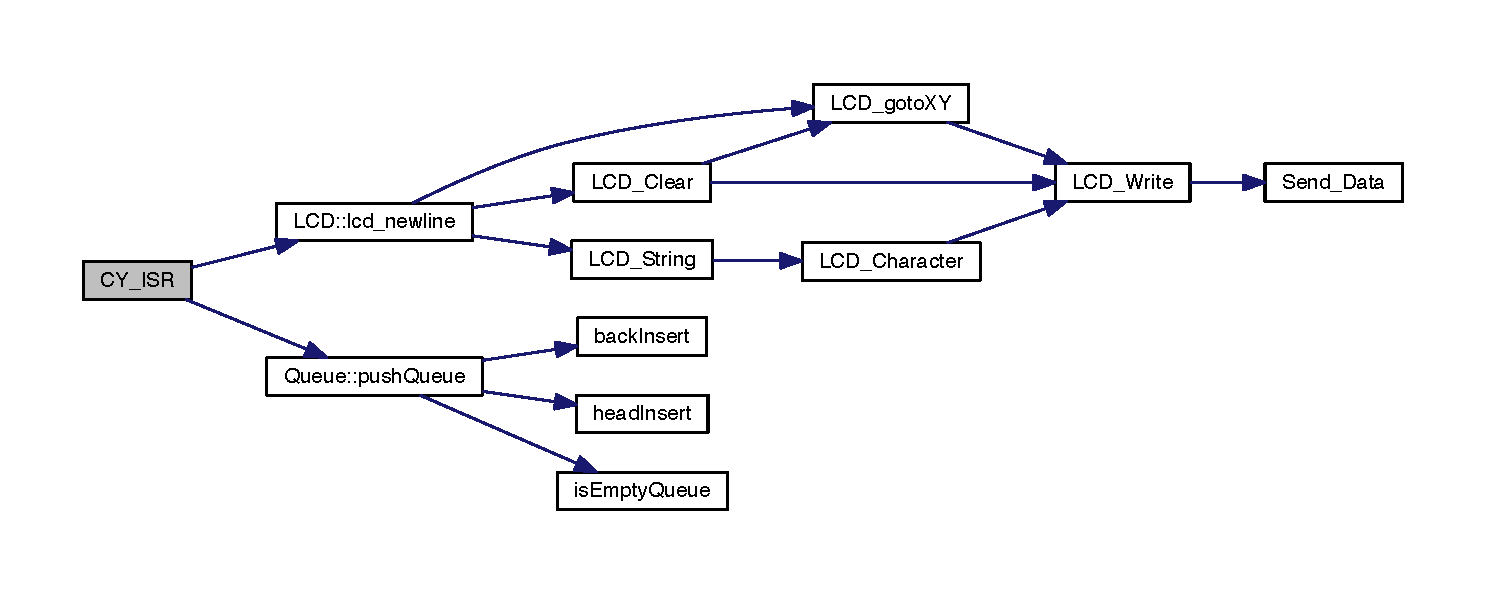
\includegraphics[width=350pt]{d3/dfe/class_s_p_i_ae65228150b9bf9ec06e2c3260dcbc328_cgraph}
\end{center}
\end{figure}


\index{S\+PI@{S\+PI}!spi\+\_\+init@{spi\+\_\+init}}
\index{spi\+\_\+init@{spi\+\_\+init}!S\+PI@{S\+PI}}
\paragraph[{\texorpdfstring{spi\+\_\+init()}{spi_init()}}]{\setlength{\rightskip}{0pt plus 5cm}void spi\+\_\+init (
\begin{DoxyParamCaption}
\item[{void}]{}
\end{DoxyParamCaption}
)}\hypertarget{class_s_p_i_a5db0aceecaf7db5fbe2984e88fef3734}{}\label{class_s_p_i_a5db0aceecaf7db5fbe2984e88fef3734}


Initialiser \hyperlink{class_s_p_i}{S\+PI} modulet. 

Initailiser \hyperlink{class_s_p_i}{S\+PI} komponent på P\+SoC\textquotesingle{}en og sætter \char`\"{}\+Custom Interrupt Handler\char`\"{}.

\begin{DoxyAuthor}{Forfatter}
Jeppe Stærk (\href{mailto:201271201@uni.au.dk}{\tt 201271201@uni.\+au.\+dk}) 
\end{DoxyAuthor}


Defineret på linje 25 i filen spi.\+c.



Refereret til af main().


\begin{DoxyCode}
26 \{
27   SPIS\_SpiUartClearTxBuffer();
28   SPIS\_SpiUartClearRxBuffer();
29   SPIS\_SetCustomInterruptHandler(isr\_spi\_rx);
30   
31   SPIS\_Start();
32 \}
\end{DoxyCode}


Her er kalder-\/grafen for denne funktion\+:\nopagebreak
\begin{figure}[H]
\begin{center}
\leavevmode
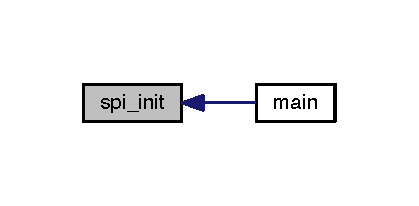
\includegraphics[width=201pt]{d3/dfe/class_s_p_i_a5db0aceecaf7db5fbe2984e88fef3734_icgraph}
\end{center}
\end{figure}




Dokumentationen for denne klasse blev genereret ud fra filerne\+:\begin{DoxyCompactItemize}
\item 
\hyperlink{spi_8h}{spi.\+h}\item 
\hyperlink{spi_8c}{spi.\+c}\end{DoxyCompactItemize}

\section{Fil-\/dokumentation}
\hypertarget{cyapicallbacks_8h}{}\subsection{cyapicallbacks.\+h filreference}
\label{cyapicallbacks_8h}\index{cyapicallbacks.\+h@{cyapicallbacks.\+h}}
Denne graf viser, hvilke filer der direkte eller indirekte inkluderer denne fil\+:
\nopagebreak
\begin{figure}[H]
\begin{center}
\leavevmode
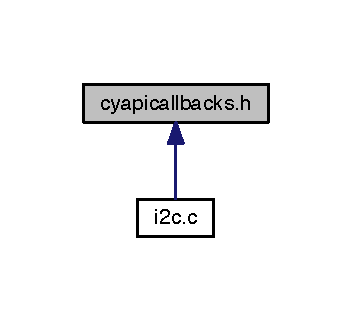
\includegraphics[width=169pt]{d4/d7d/cyapicallbacks_8h__dep__incl}
\end{center}
\end{figure}
\subsubsection*{\#Defines}
\begin{DoxyCompactItemize}
\item 
\#define \hyperlink{cyapicallbacks_8h_a696f67b7d6a9c9a1dac6387ac85b0159}{I2\+C\+S\+\_\+\+I2\+C\+\_\+\+I\+S\+R\+\_\+\+E\+X\+I\+T\+\_\+\+C\+A\+L\+L\+B\+A\+CK}
\end{DoxyCompactItemize}
\subsubsection*{Funktioner}
\begin{DoxyCompactItemize}
\item 
void \hyperlink{cyapicallbacks_8h_ab1cc1a553a438e7390297df1a2181173}{I2\+C\+S\+\_\+\+I2\+C\+\_\+\+I\+S\+R\+\_\+\+Exit\+Callback} (void)
\end{DoxyCompactItemize}


\subsubsection{\#Define-\/dokumentation}
\index{cyapicallbacks.\+h@{cyapicallbacks.\+h}!I2\+C\+S\+\_\+\+I2\+C\+\_\+\+I\+S\+R\+\_\+\+E\+X\+I\+T\+\_\+\+C\+A\+L\+L\+B\+A\+CK@{I2\+C\+S\+\_\+\+I2\+C\+\_\+\+I\+S\+R\+\_\+\+E\+X\+I\+T\+\_\+\+C\+A\+L\+L\+B\+A\+CK}}
\index{I2\+C\+S\+\_\+\+I2\+C\+\_\+\+I\+S\+R\+\_\+\+E\+X\+I\+T\+\_\+\+C\+A\+L\+L\+B\+A\+CK@{I2\+C\+S\+\_\+\+I2\+C\+\_\+\+I\+S\+R\+\_\+\+E\+X\+I\+T\+\_\+\+C\+A\+L\+L\+B\+A\+CK}!cyapicallbacks.\+h@{cyapicallbacks.\+h}}
\paragraph[{\texorpdfstring{I2\+C\+S\+\_\+\+I2\+C\+\_\+\+I\+S\+R\+\_\+\+E\+X\+I\+T\+\_\+\+C\+A\+L\+L\+B\+A\+CK}{I2CS_I2C_ISR_EXIT_CALLBACK}}]{\setlength{\rightskip}{0pt plus 5cm}\#define I2\+C\+S\+\_\+\+I2\+C\+\_\+\+I\+S\+R\+\_\+\+E\+X\+I\+T\+\_\+\+C\+A\+L\+L\+B\+A\+CK}\hypertarget{cyapicallbacks_8h_a696f67b7d6a9c9a1dac6387ac85b0159}{}\label{cyapicallbacks_8h_a696f67b7d6a9c9a1dac6387ac85b0159}


Defineret på linje 15 i filen cyapicallbacks.\+h.



\subsubsection{Funktions-\/dokumentation}
\index{cyapicallbacks.\+h@{cyapicallbacks.\+h}!I2\+C\+S\+\_\+\+I2\+C\+\_\+\+I\+S\+R\+\_\+\+Exit\+Callback@{I2\+C\+S\+\_\+\+I2\+C\+\_\+\+I\+S\+R\+\_\+\+Exit\+Callback}}
\index{I2\+C\+S\+\_\+\+I2\+C\+\_\+\+I\+S\+R\+\_\+\+Exit\+Callback@{I2\+C\+S\+\_\+\+I2\+C\+\_\+\+I\+S\+R\+\_\+\+Exit\+Callback}!cyapicallbacks.\+h@{cyapicallbacks.\+h}}
\paragraph[{\texorpdfstring{I2\+C\+S\+\_\+\+I2\+C\+\_\+\+I\+S\+R\+\_\+\+Exit\+Callback(void)}{I2CS_I2C_ISR_ExitCallback(void)}}]{\setlength{\rightskip}{0pt plus 5cm}void I2\+C\+S\+\_\+\+I2\+C\+\_\+\+I\+S\+R\+\_\+\+Exit\+Callback (
\begin{DoxyParamCaption}
\item[{void}]{}
\end{DoxyParamCaption}
)}\hypertarget{cyapicallbacks_8h_ab1cc1a553a438e7390297df1a2181173}{}\label{cyapicallbacks_8h_ab1cc1a553a438e7390297df1a2181173}

\hypertarget{data_8c}{}\subsection{data.\+c filreference}
\label{data_8c}\index{data.\+c@{data.\+c}}


\hyperlink{class_data}{Data} modul.  


{\ttfamily \#include \char`\"{}data.\+h\char`\"{}}\\*
Inklusions-\/afhængighedsgraf for data.\+c\+:
\nopagebreak
\begin{figure}[H]
\begin{center}
\leavevmode
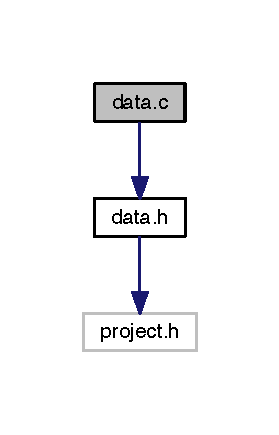
\includegraphics[width=134pt]{de/dce/data_8c__incl}
\end{center}
\end{figure}


\subsubsection{Detaljeret beskrivelse}
\hyperlink{class_data}{Data} modul. 

Indeholder data vedr. \hyperlink{class_z}{Z} modulet. \begin{DoxyAuthor}{Forfatter}
Jeppe Stærk Antonsen (\href{mailto:201271201@uni.au.dk}{\tt 201271201@uni.\+au.\+dk}) 
\end{DoxyAuthor}

\hypertarget{data_8h}{}\subsection{data.\+h filreference}
\label{data_8h}\index{data.\+h@{data.\+h}}


\hyperlink{class_data}{Data} modul.  


{\ttfamily \#include $<$project.\+h$>$}\\*
Inklusions-\/afhængighedsgraf for data.\+h\+:
\nopagebreak
\begin{figure}[H]
\begin{center}
\leavevmode
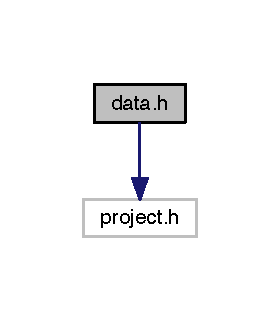
\includegraphics[width=134pt]{d6/d2b/data_8h__incl}
\end{center}
\end{figure}
Denne graf viser, hvilke filer der direkte eller indirekte inkluderer denne fil\+:
\nopagebreak
\begin{figure}[H]
\begin{center}
\leavevmode
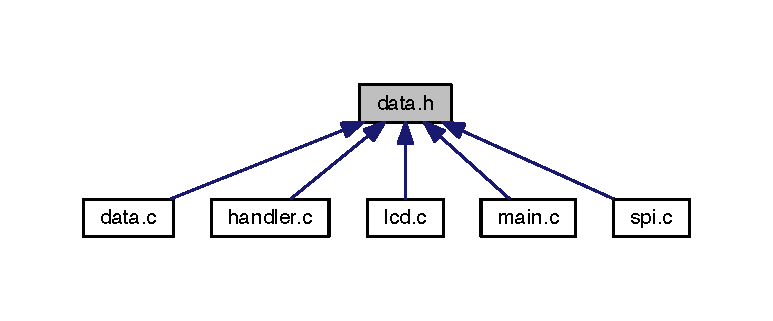
\includegraphics[width=350pt]{d2/d2f/data_8h__dep__incl}
\end{center}
\end{figure}
\subsubsection*{Datastrukturer}
\begin{DoxyCompactItemize}
\item 
struct \hyperlink{data_8h_df/d4b/struct_data_x_y}{Data\+XY}
\end{DoxyCompactItemize}
\subsubsection*{Funktioner}
\begin{DoxyCompactItemize}
\item 
void \hyperlink{data_8h_adf37c815716edf228a3cbb4564290275}{data\+\_\+init} (void)
\end{DoxyCompactItemize}
\subsubsection*{Variable}
\begin{DoxyCompactItemize}
\item 
struct \hyperlink{data_8h_df/d4b/struct_data_x_y}{Data\+XY} \hyperlink{data_8h_a89d7998a721b3f36f9f4131e7a5e42d2}{data\+XY}
\end{DoxyCompactItemize}


\subsubsection{Detaljeret beskrivelse}
\hyperlink{class_data}{Data} modul. 

Indeholder data vedr. \hyperlink{class_x_y}{XY} modulet. \begin{DoxyAuthor}{Forfatter}
Casper Dieu Le (\href{mailto:201370338@uni.au.dk}{\tt 201370338@uni.\+au.\+dk}) 

Kasper Hinkler Uldbjerg (\href{mailto:201370281@uni.au.dk}{\tt 201370281@uni.\+au.\+dk}) 

Jeppe Stærk Antonsen (\href{mailto:201271201@uni.au.dk}{\tt 201271201@uni.\+au.\+dk}) 
\end{DoxyAuthor}


\subsubsection{Datastruktur-\/documentation}
\index{Data\+XY@{Data\+XY}}\label{struct_data_x_y}
\hypertarget{data_8h_struct_data_x_y}{}
\paragraph{struct Data\+XY}


Defineret på linje 32 i filen data.\+h.



Samarbejdsdiagram for Data\+XY\+:
\nopagebreak
\begin{figure}[H]
\begin{center}
\leavevmode
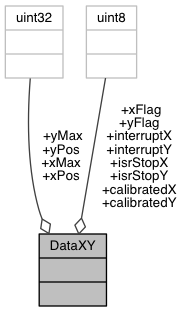
\includegraphics[width=208pt]{de/d6c/struct_data_x_y__coll__graph}
\end{center}
\end{figure}
\begin{DoxyFields}{Data-\/felter}
uint8\hypertarget{data_8h_a20403c23f502143a2dd7ee5bb641c0ab}{}\label{data_8h_a20403c23f502143a2dd7ee5bb641c0ab}
&
calibratedX&
\\
\hline

uint8\hypertarget{data_8h_adebeaa27d72b604babe006a478cfed16}{}\label{data_8h_adebeaa27d72b604babe006a478cfed16}
&
calibratedY&
\\
\hline

uint8\hypertarget{data_8h_a4cacb2964bb4b589bf79aa64a398725b}{}\label{data_8h_a4cacb2964bb4b589bf79aa64a398725b}
&
interruptX&
\\
\hline

uint8\hypertarget{data_8h_a0149ea97a32442280eb1c0b30c1eeaf1}{}\label{data_8h_a0149ea97a32442280eb1c0b30c1eeaf1}
&
interruptY&
\\
\hline

uint8\hypertarget{data_8h_ab8211b7be27d53644048a83fccb95d70}{}\label{data_8h_ab8211b7be27d53644048a83fccb95d70}
&
isr\+StopX&
\\
\hline

uint8\hypertarget{data_8h_a92ec85e6a09f5dc7ed83640f1810c4bb}{}\label{data_8h_a92ec85e6a09f5dc7ed83640f1810c4bb}
&
isr\+StopY&
\\
\hline

uint8\hypertarget{data_8h_abd60bb18cb69d4a782e0334caad9ffbc}{}\label{data_8h_abd60bb18cb69d4a782e0334caad9ffbc}
&
x\+Flag&
\\
\hline

uint32\hypertarget{data_8h_a5b6ae90a32a5f290afcc50656befceca}{}\label{data_8h_a5b6ae90a32a5f290afcc50656befceca}
&
x\+Max&
\\
\hline

uint32\hypertarget{data_8h_a5262e09f478a571552e65be75c506bdb}{}\label{data_8h_a5262e09f478a571552e65be75c506bdb}
&
x\+Pos&
\\
\hline

uint8\hypertarget{data_8h_a2093b99c34cd9ec2a282b9c4c3f61935}{}\label{data_8h_a2093b99c34cd9ec2a282b9c4c3f61935}
&
y\+Flag&
\\
\hline

uint32\hypertarget{data_8h_ab979b62fb4882313ad47718325e34879}{}\label{data_8h_ab979b62fb4882313ad47718325e34879}
&
y\+Max&
\\
\hline

uint32\hypertarget{data_8h_a4c7347df04ab0f3d860046571be08af4}{}\label{data_8h_a4c7347df04ab0f3d860046571be08af4}
&
y\+Pos&
\\
\hline

\end{DoxyFields}


\subsubsection{Funktions-\/dokumentation}
\index{data.\+h@{data.\+h}!data\+\_\+init@{data\+\_\+init}}
\index{data\+\_\+init@{data\+\_\+init}!data.\+h@{data.\+h}}
\paragraph[{\texorpdfstring{data\+\_\+init(void)}{data_init(void)}}]{\setlength{\rightskip}{0pt plus 5cm}void data\+\_\+init (
\begin{DoxyParamCaption}
\item[{void}]{}
\end{DoxyParamCaption}
)}\hypertarget{data_8h_adf37c815716edf228a3cbb4564290275}{}\label{data_8h_adf37c815716edf228a3cbb4564290275}


\subsubsection{Variabel-\/dokumentation}
\index{data.\+h@{data.\+h}!data\+XY@{data\+XY}}
\index{data\+XY@{data\+XY}!data.\+h@{data.\+h}}
\paragraph[{\texorpdfstring{data\+XY}{dataXY}}]{\setlength{\rightskip}{0pt plus 5cm}struct {\bf Data\+XY} data\+XY}\hypertarget{data_8h_a89d7998a721b3f36f9f4131e7a5e42d2}{}\label{data_8h_a89d7998a721b3f36f9f4131e7a5e42d2}


Refereret til af X\+Y\+::calibrate\+X(), X\+Y\+::calibrate\+Y(), X\+Y\+::\+C\+Y\+\_\+\+I\+S\+R(), Data\+::data\+\_\+init(), Handler\+::handler(), I2\+C\+::\+I2\+C\+S\+\_\+\+I2\+C\+\_\+\+I\+S\+R\+\_\+\+Exit\+Callback(), X\+Y\+::set\+X\+Pos(), X\+Y\+::set\+Y\+Pos() og X\+Y\+::xy\+\_\+start().


\hypertarget{handler_8c}{}\subsection{handler.\+c filreference}
\label{handler_8c}\index{handler.\+c@{handler.\+c}}


\hyperlink{class_handler}{Handler} modul.  


{\ttfamily \#include \char`\"{}handler.\+h\char`\"{}}\\*
{\ttfamily \#include \char`\"{}data.\+h\char`\"{}}\\*
{\ttfamily \#include \char`\"{}i2c.\+h\char`\"{}}\\*
{\ttfamily \#include \char`\"{}spi.\+h\char`\"{}}\\*
{\ttfamily \#include $<$stdio.\+h$>$}\\*
Inklusions-\/afhængighedsgraf for handler.\+c\+:\nopagebreak
\begin{figure}[H]
\begin{center}
\leavevmode
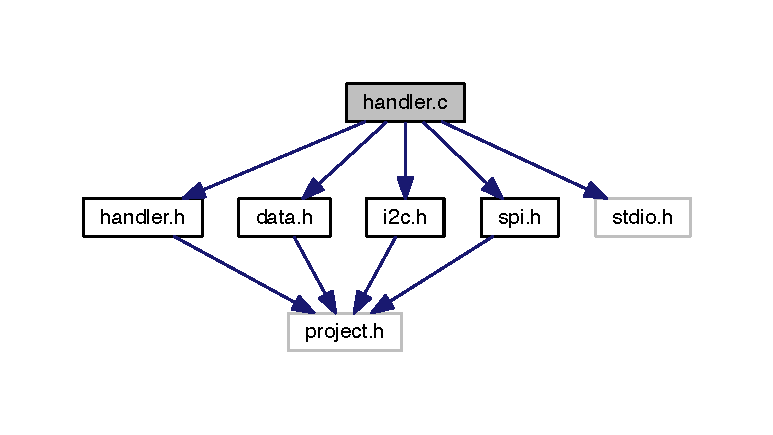
\includegraphics[width=350pt]{d2/d83/handler_8c__incl}
\end{center}
\end{figure}


\subsubsection{Detaljeret beskrivelse}
\hyperlink{class_handler}{Handler} modul. 

Håndtere indkommende kommandoer med tilhørende værdier. \begin{DoxyAuthor}{Forfatter}
Jeppe Stærk Antonsen (\href{mailto:201271201@uni.au.dk}{\tt 201271201@uni.\+au.\+dk}) 
\end{DoxyAuthor}

\hypertarget{handler_8h}{}\subsection{handler.\+h filreference}
\label{handler_8h}\index{handler.\+h@{handler.\+h}}


\hyperlink{class_handler}{Handler} modul.  


{\ttfamily \#include $<$project.\+h$>$}\\*
Inklusions-\/afhængighedsgraf for handler.\+h\+:
\nopagebreak
\begin{figure}[H]
\begin{center}
\leavevmode
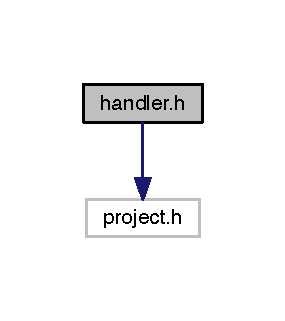
\includegraphics[width=137pt]{db/d41/handler_8h__incl}
\end{center}
\end{figure}
Denne graf viser, hvilke filer der direkte eller indirekte inkluderer denne fil\+:
\nopagebreak
\begin{figure}[H]
\begin{center}
\leavevmode
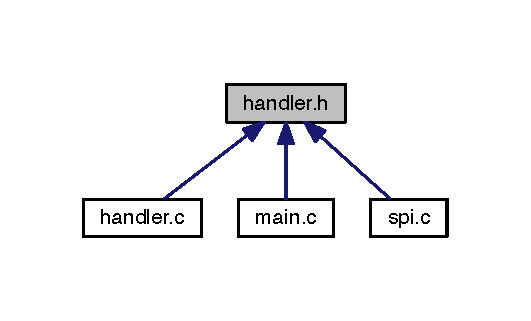
\includegraphics[width=255pt]{d4/d76/handler_8h__dep__incl}
\end{center}
\end{figure}
\subsubsection*{\#Defines}
\begin{DoxyCompactItemize}
\item 
\#define \hyperlink{handler_8h_af70b73890a98cfe329a916df037f46a4}{C\+M\+D\+\_\+\+S\+E\+T\+\_\+\+X\+\_\+\+P\+OS}~(0x10u)
\item 
\#define \hyperlink{handler_8h_a82640a671f668fb40ff4851901d5a151}{C\+M\+D\+\_\+\+S\+E\+T\+\_\+\+Y\+\_\+\+P\+OS}~(0x11u)
\item 
\#define \hyperlink{handler_8h_aa50e083669624eeaef782ebc867008f9}{C\+M\+D\+\_\+\+G\+E\+T\+\_\+\+X\+\_\+\+P\+OS}~(0x12u)
\item 
\#define \hyperlink{handler_8h_a51053e5251048d6ebbf4d2e23de40761}{C\+M\+D\+\_\+\+G\+E\+T\+\_\+\+Y\+\_\+\+P\+OS}~(0x13u)
\item 
\#define \hyperlink{handler_8h_ad9bda4ca0abdec2ab1e6506761623671}{C\+M\+D\+\_\+\+G\+E\+T\+\_\+\+X\+\_\+\+M\+AX}~(0x14u)
\item 
\#define \hyperlink{handler_8h_ab73a35345dedba2dcb9641488e8ddadd}{C\+M\+D\+\_\+\+G\+E\+T\+\_\+\+Y\+\_\+\+M\+AX}~(0x15u)
\item 
\#define \hyperlink{handler_8h_af7c8f19d1c1b9e2240251d42109c5cfd}{C\+M\+D\+\_\+\+X\+\_\+\+S\+TP}~(0x16u)
\item 
\#define \hyperlink{handler_8h_a83ab3037b2c91ea010b2d8c47acd5434}{C\+M\+D\+\_\+\+Y\+\_\+\+S\+TP}~(0x17u)
\item 
\#define \hyperlink{handler_8h_a5edf35288955238e1090f2367f96e828}{C\+M\+D\+\_\+\+X\+\_\+\+C\+AL}~(0x18u)
\item 
\#define \hyperlink{handler_8h_a2b2db51eef91dc2aa5586d0817838ef2}{C\+M\+D\+\_\+\+Y\+\_\+\+C\+AL}~(0x19u)
\item 
\#define \hyperlink{handler_8h_a6e695093ea021ccac7cc5d2d788095c9}{C\+M\+D\+\_\+\+S\+E\+T\+\_\+\+Z\+\_\+\+P\+OS}~(0x20u)
\item 
\#define \hyperlink{handler_8h_a4d76e78d09a00f75609569d9aa92ab98}{C\+M\+D\+\_\+\+G\+E\+T\+\_\+\+Z\+\_\+\+P\+OS}~(0x21u)
\item 
\#define \hyperlink{handler_8h_a188e7cab5d0cf0e363a20c5abcdab482}{C\+M\+D\+\_\+\+G\+E\+T\+\_\+\+Z\+\_\+\+M\+AX}~(0x22u)
\item 
\#define \hyperlink{handler_8h_ad119aef78e8cb8e9aa12f35aeae94a99}{C\+M\+D\+\_\+\+Z\+\_\+\+S\+TP}~(0x23u)
\item 
\#define \hyperlink{handler_8h_ab77bdaae57e9e34f7bfc1d1a31213f94}{C\+M\+D\+\_\+\+Z\+\_\+\+C\+AL}~(0x24u)
\item 
\#define \hyperlink{handler_8h_afc24de4a99d70315d939185a1c3d61f0}{C\+M\+D\+\_\+\+S\+E\+T\+\_\+\+R\+E\+D\+\_\+\+V\+AL}~(0x30u)
\item 
\#define \hyperlink{handler_8h_a24acd29fea2e546409449638b79ac094}{C\+M\+D\+\_\+\+S\+E\+T\+\_\+\+G\+R\+E\+E\+N\+\_\+\+V\+AL}~(0x31u)
\item 
\#define \hyperlink{handler_8h_a4ab3ea64ee56aef3a566698b8959df51}{C\+M\+D\+\_\+\+S\+E\+T\+\_\+\+B\+L\+U\+E\+\_\+\+V\+AL}~(0x32u)
\item 
\#define \hyperlink{handler_8h_a3f217d17f4b67e6b46eb294ab3db2e87}{C\+M\+D\+\_\+\+S\+E\+T\+\_\+\+L\+U\+M\+E\+N\+\_\+\+V\+AL}~(0x33u)
\item 
\#define \hyperlink{handler_8h_a1fe6f15c7c98032dc2bd2a1417977fcf}{C\+M\+D\+\_\+\+S\+E\+T\+\_\+\+P\+O\+W\+E\+R\+\_\+\+S\+TS}~(0x34u)
\item 
\#define \hyperlink{handler_8h_aa2f09e60c4eeae4560da88c6b1b08c60}{C\+M\+D\+\_\+\+G\+E\+T\+\_\+\+R\+E\+D\+\_\+\+V\+AL}~(0x35u)
\item 
\#define \hyperlink{handler_8h_a55d24f50aeb52afddd491d97a66c81ef}{C\+M\+D\+\_\+\+G\+E\+T\+\_\+\+G\+R\+E\+E\+N\+\_\+\+V\+AL}~(0x36u)
\item 
\#define \hyperlink{handler_8h_a81052c67f996705d7eacfcea66bdde08}{C\+M\+D\+\_\+\+G\+E\+T\+\_\+\+B\+L\+U\+E\+\_\+\+V\+AL}~(0x37u)
\item 
\#define \hyperlink{handler_8h_a8ed7ad21a658c878390e9cec4d45aab5}{C\+M\+D\+\_\+\+G\+E\+T\+\_\+\+L\+U\+M\+E\+N\+\_\+\+V\+AL}~(0x38u)
\item 
\#define \hyperlink{handler_8h_ab9e8683e41e93fd467b170c321a1c685}{C\+M\+D\+\_\+\+G\+E\+T\+\_\+\+P\+O\+W\+E\+R\+\_\+\+S\+TS}~(0x39u)
\item 
\#define \hyperlink{handler_8h_a67cc7e7270e79a6e95be2e25cac29feb}{C\+M\+D\+\_\+\+S\+E\+T\+\_\+\+D\+I\+S\+T\+A\+N\+C\+E\+\_\+\+S\+TS}~(0x40u)
\item 
\#define \hyperlink{handler_8h_a84f8a23b131cb2b163e16889afd9ef85}{C\+M\+D\+\_\+\+S\+E\+T\+\_\+\+M\+O\+V\+E\+M\+E\+N\+T\+\_\+\+S\+TS}~(0x41u)
\item 
\#define \hyperlink{handler_8h_a8ea17eed84662f9389bfa1751c03a4b2}{C\+M\+D\+\_\+\+G\+E\+T\+\_\+\+D\+I\+S\+T\+A\+N\+C\+E\+\_\+\+S\+TS}~(0x42u)
\item 
\#define \hyperlink{handler_8h_a4adcfb68de1b319e19342143cb61b550}{C\+M\+D\+\_\+\+G\+E\+T\+\_\+\+M\+O\+V\+E\+M\+E\+N\+T\+\_\+\+S\+TS}~(0x43u)
\item 
\#define \hyperlink{handler_8h_a17dc606d3dbd6f9d4ca831cb02c91af0}{C\+M\+D\+\_\+\+D\+I\+S\+T\+A\+N\+C\+E\+\_\+\+A\+L\+RT}~(0x44u)
\item 
\#define \hyperlink{handler_8h_a7bd43223cfa796f0289d0548e090bbcc}{C\+M\+D\+\_\+\+M\+O\+V\+E\+M\+E\+N\+T\+\_\+\+A\+L\+RT}~(0x45u)
\end{DoxyCompactItemize}
\subsubsection*{Funktioner}
\begin{DoxyCompactItemize}
\item 
void \hyperlink{handler_8h_af5be5b016b862943cd22504490acc8f4}{handler} (uint8 cmd, uint8 val)
\end{DoxyCompactItemize}


\subsubsection{Detaljeret beskrivelse}
\hyperlink{class_handler}{Handler} modul. 

Håndtere indkommende kommandoer med tilhørende værdier. \begin{DoxyAuthor}{Forfatter}
Jeppe Stærk Antonsen (\href{mailto:201271201@uni.au.dk}{\tt 201271201@uni.\+au.\+dk}) 
\end{DoxyAuthor}


\subsubsection{\#Define-\/dokumentation}
\index{handler.\+h@{handler.\+h}!C\+M\+D\+\_\+\+D\+I\+S\+T\+A\+N\+C\+E\+\_\+\+A\+L\+RT@{C\+M\+D\+\_\+\+D\+I\+S\+T\+A\+N\+C\+E\+\_\+\+A\+L\+RT}}
\index{C\+M\+D\+\_\+\+D\+I\+S\+T\+A\+N\+C\+E\+\_\+\+A\+L\+RT@{C\+M\+D\+\_\+\+D\+I\+S\+T\+A\+N\+C\+E\+\_\+\+A\+L\+RT}!handler.\+h@{handler.\+h}}
\paragraph[{\texorpdfstring{C\+M\+D\+\_\+\+D\+I\+S\+T\+A\+N\+C\+E\+\_\+\+A\+L\+RT}{CMD_DISTANCE_ALRT}}]{\setlength{\rightskip}{0pt plus 5cm}\#define C\+M\+D\+\_\+\+D\+I\+S\+T\+A\+N\+C\+E\+\_\+\+A\+L\+RT~(0x44u)}\hypertarget{handler_8h_a17dc606d3dbd6f9d4ca831cb02c91af0}{}\label{handler_8h_a17dc606d3dbd6f9d4ca831cb02c91af0}


Defineret på linje 65 i filen handler.\+h.



Refereret til af Handler\+::handler().

\index{handler.\+h@{handler.\+h}!C\+M\+D\+\_\+\+G\+E\+T\+\_\+\+B\+L\+U\+E\+\_\+\+V\+AL@{C\+M\+D\+\_\+\+G\+E\+T\+\_\+\+B\+L\+U\+E\+\_\+\+V\+AL}}
\index{C\+M\+D\+\_\+\+G\+E\+T\+\_\+\+B\+L\+U\+E\+\_\+\+V\+AL@{C\+M\+D\+\_\+\+G\+E\+T\+\_\+\+B\+L\+U\+E\+\_\+\+V\+AL}!handler.\+h@{handler.\+h}}
\paragraph[{\texorpdfstring{C\+M\+D\+\_\+\+G\+E\+T\+\_\+\+B\+L\+U\+E\+\_\+\+V\+AL}{CMD_GET_BLUE_VAL}}]{\setlength{\rightskip}{0pt plus 5cm}\#define C\+M\+D\+\_\+\+G\+E\+T\+\_\+\+B\+L\+U\+E\+\_\+\+V\+AL~(0x37u)}\hypertarget{handler_8h_a81052c67f996705d7eacfcea66bdde08}{}\label{handler_8h_a81052c67f996705d7eacfcea66bdde08}


Defineret på linje 58 i filen handler.\+h.



Refereret til af S\+P\+I\+::\+C\+Y\+\_\+\+I\+S\+R() og Handler\+::handler().

\index{handler.\+h@{handler.\+h}!C\+M\+D\+\_\+\+G\+E\+T\+\_\+\+D\+I\+S\+T\+A\+N\+C\+E\+\_\+\+S\+TS@{C\+M\+D\+\_\+\+G\+E\+T\+\_\+\+D\+I\+S\+T\+A\+N\+C\+E\+\_\+\+S\+TS}}
\index{C\+M\+D\+\_\+\+G\+E\+T\+\_\+\+D\+I\+S\+T\+A\+N\+C\+E\+\_\+\+S\+TS@{C\+M\+D\+\_\+\+G\+E\+T\+\_\+\+D\+I\+S\+T\+A\+N\+C\+E\+\_\+\+S\+TS}!handler.\+h@{handler.\+h}}
\paragraph[{\texorpdfstring{C\+M\+D\+\_\+\+G\+E\+T\+\_\+\+D\+I\+S\+T\+A\+N\+C\+E\+\_\+\+S\+TS}{CMD_GET_DISTANCE_STS}}]{\setlength{\rightskip}{0pt plus 5cm}\#define C\+M\+D\+\_\+\+G\+E\+T\+\_\+\+D\+I\+S\+T\+A\+N\+C\+E\+\_\+\+S\+TS~(0x42u)}\hypertarget{handler_8h_a8ea17eed84662f9389bfa1751c03a4b2}{}\label{handler_8h_a8ea17eed84662f9389bfa1751c03a4b2}


Defineret på linje 63 i filen handler.\+h.



Refereret til af Handler\+::handler().

\index{handler.\+h@{handler.\+h}!C\+M\+D\+\_\+\+G\+E\+T\+\_\+\+G\+R\+E\+E\+N\+\_\+\+V\+AL@{C\+M\+D\+\_\+\+G\+E\+T\+\_\+\+G\+R\+E\+E\+N\+\_\+\+V\+AL}}
\index{C\+M\+D\+\_\+\+G\+E\+T\+\_\+\+G\+R\+E\+E\+N\+\_\+\+V\+AL@{C\+M\+D\+\_\+\+G\+E\+T\+\_\+\+G\+R\+E\+E\+N\+\_\+\+V\+AL}!handler.\+h@{handler.\+h}}
\paragraph[{\texorpdfstring{C\+M\+D\+\_\+\+G\+E\+T\+\_\+\+G\+R\+E\+E\+N\+\_\+\+V\+AL}{CMD_GET_GREEN_VAL}}]{\setlength{\rightskip}{0pt plus 5cm}\#define C\+M\+D\+\_\+\+G\+E\+T\+\_\+\+G\+R\+E\+E\+N\+\_\+\+V\+AL~(0x36u)}\hypertarget{handler_8h_a55d24f50aeb52afddd491d97a66c81ef}{}\label{handler_8h_a55d24f50aeb52afddd491d97a66c81ef}


Defineret på linje 57 i filen handler.\+h.



Refereret til af S\+P\+I\+::\+C\+Y\+\_\+\+I\+S\+R() og Handler\+::handler().

\index{handler.\+h@{handler.\+h}!C\+M\+D\+\_\+\+G\+E\+T\+\_\+\+L\+U\+M\+E\+N\+\_\+\+V\+AL@{C\+M\+D\+\_\+\+G\+E\+T\+\_\+\+L\+U\+M\+E\+N\+\_\+\+V\+AL}}
\index{C\+M\+D\+\_\+\+G\+E\+T\+\_\+\+L\+U\+M\+E\+N\+\_\+\+V\+AL@{C\+M\+D\+\_\+\+G\+E\+T\+\_\+\+L\+U\+M\+E\+N\+\_\+\+V\+AL}!handler.\+h@{handler.\+h}}
\paragraph[{\texorpdfstring{C\+M\+D\+\_\+\+G\+E\+T\+\_\+\+L\+U\+M\+E\+N\+\_\+\+V\+AL}{CMD_GET_LUMEN_VAL}}]{\setlength{\rightskip}{0pt plus 5cm}\#define C\+M\+D\+\_\+\+G\+E\+T\+\_\+\+L\+U\+M\+E\+N\+\_\+\+V\+AL~(0x38u)}\hypertarget{handler_8h_a8ed7ad21a658c878390e9cec4d45aab5}{}\label{handler_8h_a8ed7ad21a658c878390e9cec4d45aab5}


Defineret på linje 59 i filen handler.\+h.



Refereret til af Handler\+::handler().

\index{handler.\+h@{handler.\+h}!C\+M\+D\+\_\+\+G\+E\+T\+\_\+\+M\+O\+V\+E\+M\+E\+N\+T\+\_\+\+S\+TS@{C\+M\+D\+\_\+\+G\+E\+T\+\_\+\+M\+O\+V\+E\+M\+E\+N\+T\+\_\+\+S\+TS}}
\index{C\+M\+D\+\_\+\+G\+E\+T\+\_\+\+M\+O\+V\+E\+M\+E\+N\+T\+\_\+\+S\+TS@{C\+M\+D\+\_\+\+G\+E\+T\+\_\+\+M\+O\+V\+E\+M\+E\+N\+T\+\_\+\+S\+TS}!handler.\+h@{handler.\+h}}
\paragraph[{\texorpdfstring{C\+M\+D\+\_\+\+G\+E\+T\+\_\+\+M\+O\+V\+E\+M\+E\+N\+T\+\_\+\+S\+TS}{CMD_GET_MOVEMENT_STS}}]{\setlength{\rightskip}{0pt plus 5cm}\#define C\+M\+D\+\_\+\+G\+E\+T\+\_\+\+M\+O\+V\+E\+M\+E\+N\+T\+\_\+\+S\+TS~(0x43u)}\hypertarget{handler_8h_a4adcfb68de1b319e19342143cb61b550}{}\label{handler_8h_a4adcfb68de1b319e19342143cb61b550}


Defineret på linje 64 i filen handler.\+h.



Refereret til af Handler\+::handler().

\index{handler.\+h@{handler.\+h}!C\+M\+D\+\_\+\+G\+E\+T\+\_\+\+P\+O\+W\+E\+R\+\_\+\+S\+TS@{C\+M\+D\+\_\+\+G\+E\+T\+\_\+\+P\+O\+W\+E\+R\+\_\+\+S\+TS}}
\index{C\+M\+D\+\_\+\+G\+E\+T\+\_\+\+P\+O\+W\+E\+R\+\_\+\+S\+TS@{C\+M\+D\+\_\+\+G\+E\+T\+\_\+\+P\+O\+W\+E\+R\+\_\+\+S\+TS}!handler.\+h@{handler.\+h}}
\paragraph[{\texorpdfstring{C\+M\+D\+\_\+\+G\+E\+T\+\_\+\+P\+O\+W\+E\+R\+\_\+\+S\+TS}{CMD_GET_POWER_STS}}]{\setlength{\rightskip}{0pt plus 5cm}\#define C\+M\+D\+\_\+\+G\+E\+T\+\_\+\+P\+O\+W\+E\+R\+\_\+\+S\+TS~(0x39u)}\hypertarget{handler_8h_ab9e8683e41e93fd467b170c321a1c685}{}\label{handler_8h_ab9e8683e41e93fd467b170c321a1c685}


Defineret på linje 60 i filen handler.\+h.



Refereret til af Handler\+::handler().

\index{handler.\+h@{handler.\+h}!C\+M\+D\+\_\+\+G\+E\+T\+\_\+\+R\+E\+D\+\_\+\+V\+AL@{C\+M\+D\+\_\+\+G\+E\+T\+\_\+\+R\+E\+D\+\_\+\+V\+AL}}
\index{C\+M\+D\+\_\+\+G\+E\+T\+\_\+\+R\+E\+D\+\_\+\+V\+AL@{C\+M\+D\+\_\+\+G\+E\+T\+\_\+\+R\+E\+D\+\_\+\+V\+AL}!handler.\+h@{handler.\+h}}
\paragraph[{\texorpdfstring{C\+M\+D\+\_\+\+G\+E\+T\+\_\+\+R\+E\+D\+\_\+\+V\+AL}{CMD_GET_RED_VAL}}]{\setlength{\rightskip}{0pt plus 5cm}\#define C\+M\+D\+\_\+\+G\+E\+T\+\_\+\+R\+E\+D\+\_\+\+V\+AL~(0x35u)}\hypertarget{handler_8h_aa2f09e60c4eeae4560da88c6b1b08c60}{}\label{handler_8h_aa2f09e60c4eeae4560da88c6b1b08c60}


Defineret på linje 56 i filen handler.\+h.



Refereret til af S\+P\+I\+::\+C\+Y\+\_\+\+I\+S\+R() og Handler\+::handler().

\index{handler.\+h@{handler.\+h}!C\+M\+D\+\_\+\+G\+E\+T\+\_\+\+X\+\_\+\+M\+AX@{C\+M\+D\+\_\+\+G\+E\+T\+\_\+\+X\+\_\+\+M\+AX}}
\index{C\+M\+D\+\_\+\+G\+E\+T\+\_\+\+X\+\_\+\+M\+AX@{C\+M\+D\+\_\+\+G\+E\+T\+\_\+\+X\+\_\+\+M\+AX}!handler.\+h@{handler.\+h}}
\paragraph[{\texorpdfstring{C\+M\+D\+\_\+\+G\+E\+T\+\_\+\+X\+\_\+\+M\+AX}{CMD_GET_X_MAX}}]{\setlength{\rightskip}{0pt plus 5cm}\#define C\+M\+D\+\_\+\+G\+E\+T\+\_\+\+X\+\_\+\+M\+AX~(0x14u)}\hypertarget{handler_8h_ad9bda4ca0abdec2ab1e6506761623671}{}\label{handler_8h_ad9bda4ca0abdec2ab1e6506761623671}


Defineret på linje 40 i filen handler.\+h.

\index{handler.\+h@{handler.\+h}!C\+M\+D\+\_\+\+G\+E\+T\+\_\+\+X\+\_\+\+P\+OS@{C\+M\+D\+\_\+\+G\+E\+T\+\_\+\+X\+\_\+\+P\+OS}}
\index{C\+M\+D\+\_\+\+G\+E\+T\+\_\+\+X\+\_\+\+P\+OS@{C\+M\+D\+\_\+\+G\+E\+T\+\_\+\+X\+\_\+\+P\+OS}!handler.\+h@{handler.\+h}}
\paragraph[{\texorpdfstring{C\+M\+D\+\_\+\+G\+E\+T\+\_\+\+X\+\_\+\+P\+OS}{CMD_GET_X_POS}}]{\setlength{\rightskip}{0pt plus 5cm}\#define C\+M\+D\+\_\+\+G\+E\+T\+\_\+\+X\+\_\+\+P\+OS~(0x12u)}\hypertarget{handler_8h_aa50e083669624eeaef782ebc867008f9}{}\label{handler_8h_aa50e083669624eeaef782ebc867008f9}


Defineret på linje 38 i filen handler.\+h.



Refereret til af S\+P\+I\+::\+C\+Y\+\_\+\+I\+S\+R() og Handler\+::handler().

\index{handler.\+h@{handler.\+h}!C\+M\+D\+\_\+\+G\+E\+T\+\_\+\+Y\+\_\+\+M\+AX@{C\+M\+D\+\_\+\+G\+E\+T\+\_\+\+Y\+\_\+\+M\+AX}}
\index{C\+M\+D\+\_\+\+G\+E\+T\+\_\+\+Y\+\_\+\+M\+AX@{C\+M\+D\+\_\+\+G\+E\+T\+\_\+\+Y\+\_\+\+M\+AX}!handler.\+h@{handler.\+h}}
\paragraph[{\texorpdfstring{C\+M\+D\+\_\+\+G\+E\+T\+\_\+\+Y\+\_\+\+M\+AX}{CMD_GET_Y_MAX}}]{\setlength{\rightskip}{0pt plus 5cm}\#define C\+M\+D\+\_\+\+G\+E\+T\+\_\+\+Y\+\_\+\+M\+AX~(0x15u)}\hypertarget{handler_8h_ab73a35345dedba2dcb9641488e8ddadd}{}\label{handler_8h_ab73a35345dedba2dcb9641488e8ddadd}


Defineret på linje 41 i filen handler.\+h.

\index{handler.\+h@{handler.\+h}!C\+M\+D\+\_\+\+G\+E\+T\+\_\+\+Y\+\_\+\+P\+OS@{C\+M\+D\+\_\+\+G\+E\+T\+\_\+\+Y\+\_\+\+P\+OS}}
\index{C\+M\+D\+\_\+\+G\+E\+T\+\_\+\+Y\+\_\+\+P\+OS@{C\+M\+D\+\_\+\+G\+E\+T\+\_\+\+Y\+\_\+\+P\+OS}!handler.\+h@{handler.\+h}}
\paragraph[{\texorpdfstring{C\+M\+D\+\_\+\+G\+E\+T\+\_\+\+Y\+\_\+\+P\+OS}{CMD_GET_Y_POS}}]{\setlength{\rightskip}{0pt plus 5cm}\#define C\+M\+D\+\_\+\+G\+E\+T\+\_\+\+Y\+\_\+\+P\+OS~(0x13u)}\hypertarget{handler_8h_a51053e5251048d6ebbf4d2e23de40761}{}\label{handler_8h_a51053e5251048d6ebbf4d2e23de40761}


Defineret på linje 39 i filen handler.\+h.



Refereret til af S\+P\+I\+::\+C\+Y\+\_\+\+I\+S\+R() og Handler\+::handler().

\index{handler.\+h@{handler.\+h}!C\+M\+D\+\_\+\+G\+E\+T\+\_\+\+Z\+\_\+\+M\+AX@{C\+M\+D\+\_\+\+G\+E\+T\+\_\+\+Z\+\_\+\+M\+AX}}
\index{C\+M\+D\+\_\+\+G\+E\+T\+\_\+\+Z\+\_\+\+M\+AX@{C\+M\+D\+\_\+\+G\+E\+T\+\_\+\+Z\+\_\+\+M\+AX}!handler.\+h@{handler.\+h}}
\paragraph[{\texorpdfstring{C\+M\+D\+\_\+\+G\+E\+T\+\_\+\+Z\+\_\+\+M\+AX}{CMD_GET_Z_MAX}}]{\setlength{\rightskip}{0pt plus 5cm}\#define C\+M\+D\+\_\+\+G\+E\+T\+\_\+\+Z\+\_\+\+M\+AX~(0x22u)}\hypertarget{handler_8h_a188e7cab5d0cf0e363a20c5abcdab482}{}\label{handler_8h_a188e7cab5d0cf0e363a20c5abcdab482}


Defineret på linje 48 i filen handler.\+h.

\index{handler.\+h@{handler.\+h}!C\+M\+D\+\_\+\+G\+E\+T\+\_\+\+Z\+\_\+\+P\+OS@{C\+M\+D\+\_\+\+G\+E\+T\+\_\+\+Z\+\_\+\+P\+OS}}
\index{C\+M\+D\+\_\+\+G\+E\+T\+\_\+\+Z\+\_\+\+P\+OS@{C\+M\+D\+\_\+\+G\+E\+T\+\_\+\+Z\+\_\+\+P\+OS}!handler.\+h@{handler.\+h}}
\paragraph[{\texorpdfstring{C\+M\+D\+\_\+\+G\+E\+T\+\_\+\+Z\+\_\+\+P\+OS}{CMD_GET_Z_POS}}]{\setlength{\rightskip}{0pt plus 5cm}\#define C\+M\+D\+\_\+\+G\+E\+T\+\_\+\+Z\+\_\+\+P\+OS~(0x21u)}\hypertarget{handler_8h_a4d76e78d09a00f75609569d9aa92ab98}{}\label{handler_8h_a4d76e78d09a00f75609569d9aa92ab98}


Defineret på linje 47 i filen handler.\+h.



Refereret til af S\+P\+I\+::\+C\+Y\+\_\+\+I\+S\+R() og Handler\+::handler().

\index{handler.\+h@{handler.\+h}!C\+M\+D\+\_\+\+M\+O\+V\+E\+M\+E\+N\+T\+\_\+\+A\+L\+RT@{C\+M\+D\+\_\+\+M\+O\+V\+E\+M\+E\+N\+T\+\_\+\+A\+L\+RT}}
\index{C\+M\+D\+\_\+\+M\+O\+V\+E\+M\+E\+N\+T\+\_\+\+A\+L\+RT@{C\+M\+D\+\_\+\+M\+O\+V\+E\+M\+E\+N\+T\+\_\+\+A\+L\+RT}!handler.\+h@{handler.\+h}}
\paragraph[{\texorpdfstring{C\+M\+D\+\_\+\+M\+O\+V\+E\+M\+E\+N\+T\+\_\+\+A\+L\+RT}{CMD_MOVEMENT_ALRT}}]{\setlength{\rightskip}{0pt plus 5cm}\#define C\+M\+D\+\_\+\+M\+O\+V\+E\+M\+E\+N\+T\+\_\+\+A\+L\+RT~(0x45u)}\hypertarget{handler_8h_a7bd43223cfa796f0289d0548e090bbcc}{}\label{handler_8h_a7bd43223cfa796f0289d0548e090bbcc}


Defineret på linje 66 i filen handler.\+h.



Refereret til af Handler\+::handler().

\index{handler.\+h@{handler.\+h}!C\+M\+D\+\_\+\+S\+E\+T\+\_\+\+B\+L\+U\+E\+\_\+\+V\+AL@{C\+M\+D\+\_\+\+S\+E\+T\+\_\+\+B\+L\+U\+E\+\_\+\+V\+AL}}
\index{C\+M\+D\+\_\+\+S\+E\+T\+\_\+\+B\+L\+U\+E\+\_\+\+V\+AL@{C\+M\+D\+\_\+\+S\+E\+T\+\_\+\+B\+L\+U\+E\+\_\+\+V\+AL}!handler.\+h@{handler.\+h}}
\paragraph[{\texorpdfstring{C\+M\+D\+\_\+\+S\+E\+T\+\_\+\+B\+L\+U\+E\+\_\+\+V\+AL}{CMD_SET_BLUE_VAL}}]{\setlength{\rightskip}{0pt plus 5cm}\#define C\+M\+D\+\_\+\+S\+E\+T\+\_\+\+B\+L\+U\+E\+\_\+\+V\+AL~(0x32u)}\hypertarget{handler_8h_a4ab3ea64ee56aef3a566698b8959df51}{}\label{handler_8h_a4ab3ea64ee56aef3a566698b8959df51}


Defineret på linje 53 i filen handler.\+h.



Refereret til af Handler\+::handler().

\index{handler.\+h@{handler.\+h}!C\+M\+D\+\_\+\+S\+E\+T\+\_\+\+D\+I\+S\+T\+A\+N\+C\+E\+\_\+\+S\+TS@{C\+M\+D\+\_\+\+S\+E\+T\+\_\+\+D\+I\+S\+T\+A\+N\+C\+E\+\_\+\+S\+TS}}
\index{C\+M\+D\+\_\+\+S\+E\+T\+\_\+\+D\+I\+S\+T\+A\+N\+C\+E\+\_\+\+S\+TS@{C\+M\+D\+\_\+\+S\+E\+T\+\_\+\+D\+I\+S\+T\+A\+N\+C\+E\+\_\+\+S\+TS}!handler.\+h@{handler.\+h}}
\paragraph[{\texorpdfstring{C\+M\+D\+\_\+\+S\+E\+T\+\_\+\+D\+I\+S\+T\+A\+N\+C\+E\+\_\+\+S\+TS}{CMD_SET_DISTANCE_STS}}]{\setlength{\rightskip}{0pt plus 5cm}\#define C\+M\+D\+\_\+\+S\+E\+T\+\_\+\+D\+I\+S\+T\+A\+N\+C\+E\+\_\+\+S\+TS~(0x40u)}\hypertarget{handler_8h_a67cc7e7270e79a6e95be2e25cac29feb}{}\label{handler_8h_a67cc7e7270e79a6e95be2e25cac29feb}


Defineret på linje 61 i filen handler.\+h.



Refereret til af Handler\+::handler().

\index{handler.\+h@{handler.\+h}!C\+M\+D\+\_\+\+S\+E\+T\+\_\+\+G\+R\+E\+E\+N\+\_\+\+V\+AL@{C\+M\+D\+\_\+\+S\+E\+T\+\_\+\+G\+R\+E\+E\+N\+\_\+\+V\+AL}}
\index{C\+M\+D\+\_\+\+S\+E\+T\+\_\+\+G\+R\+E\+E\+N\+\_\+\+V\+AL@{C\+M\+D\+\_\+\+S\+E\+T\+\_\+\+G\+R\+E\+E\+N\+\_\+\+V\+AL}!handler.\+h@{handler.\+h}}
\paragraph[{\texorpdfstring{C\+M\+D\+\_\+\+S\+E\+T\+\_\+\+G\+R\+E\+E\+N\+\_\+\+V\+AL}{CMD_SET_GREEN_VAL}}]{\setlength{\rightskip}{0pt plus 5cm}\#define C\+M\+D\+\_\+\+S\+E\+T\+\_\+\+G\+R\+E\+E\+N\+\_\+\+V\+AL~(0x31u)}\hypertarget{handler_8h_a24acd29fea2e546409449638b79ac094}{}\label{handler_8h_a24acd29fea2e546409449638b79ac094}


Defineret på linje 52 i filen handler.\+h.



Refereret til af Handler\+::handler().

\index{handler.\+h@{handler.\+h}!C\+M\+D\+\_\+\+S\+E\+T\+\_\+\+L\+U\+M\+E\+N\+\_\+\+V\+AL@{C\+M\+D\+\_\+\+S\+E\+T\+\_\+\+L\+U\+M\+E\+N\+\_\+\+V\+AL}}
\index{C\+M\+D\+\_\+\+S\+E\+T\+\_\+\+L\+U\+M\+E\+N\+\_\+\+V\+AL@{C\+M\+D\+\_\+\+S\+E\+T\+\_\+\+L\+U\+M\+E\+N\+\_\+\+V\+AL}!handler.\+h@{handler.\+h}}
\paragraph[{\texorpdfstring{C\+M\+D\+\_\+\+S\+E\+T\+\_\+\+L\+U\+M\+E\+N\+\_\+\+V\+AL}{CMD_SET_LUMEN_VAL}}]{\setlength{\rightskip}{0pt plus 5cm}\#define C\+M\+D\+\_\+\+S\+E\+T\+\_\+\+L\+U\+M\+E\+N\+\_\+\+V\+AL~(0x33u)}\hypertarget{handler_8h_a3f217d17f4b67e6b46eb294ab3db2e87}{}\label{handler_8h_a3f217d17f4b67e6b46eb294ab3db2e87}


Defineret på linje 54 i filen handler.\+h.



Refereret til af Handler\+::handler().

\index{handler.\+h@{handler.\+h}!C\+M\+D\+\_\+\+S\+E\+T\+\_\+\+M\+O\+V\+E\+M\+E\+N\+T\+\_\+\+S\+TS@{C\+M\+D\+\_\+\+S\+E\+T\+\_\+\+M\+O\+V\+E\+M\+E\+N\+T\+\_\+\+S\+TS}}
\index{C\+M\+D\+\_\+\+S\+E\+T\+\_\+\+M\+O\+V\+E\+M\+E\+N\+T\+\_\+\+S\+TS@{C\+M\+D\+\_\+\+S\+E\+T\+\_\+\+M\+O\+V\+E\+M\+E\+N\+T\+\_\+\+S\+TS}!handler.\+h@{handler.\+h}}
\paragraph[{\texorpdfstring{C\+M\+D\+\_\+\+S\+E\+T\+\_\+\+M\+O\+V\+E\+M\+E\+N\+T\+\_\+\+S\+TS}{CMD_SET_MOVEMENT_STS}}]{\setlength{\rightskip}{0pt plus 5cm}\#define C\+M\+D\+\_\+\+S\+E\+T\+\_\+\+M\+O\+V\+E\+M\+E\+N\+T\+\_\+\+S\+TS~(0x41u)}\hypertarget{handler_8h_a84f8a23b131cb2b163e16889afd9ef85}{}\label{handler_8h_a84f8a23b131cb2b163e16889afd9ef85}


Defineret på linje 62 i filen handler.\+h.



Refereret til af Handler\+::handler().

\index{handler.\+h@{handler.\+h}!C\+M\+D\+\_\+\+S\+E\+T\+\_\+\+P\+O\+W\+E\+R\+\_\+\+S\+TS@{C\+M\+D\+\_\+\+S\+E\+T\+\_\+\+P\+O\+W\+E\+R\+\_\+\+S\+TS}}
\index{C\+M\+D\+\_\+\+S\+E\+T\+\_\+\+P\+O\+W\+E\+R\+\_\+\+S\+TS@{C\+M\+D\+\_\+\+S\+E\+T\+\_\+\+P\+O\+W\+E\+R\+\_\+\+S\+TS}!handler.\+h@{handler.\+h}}
\paragraph[{\texorpdfstring{C\+M\+D\+\_\+\+S\+E\+T\+\_\+\+P\+O\+W\+E\+R\+\_\+\+S\+TS}{CMD_SET_POWER_STS}}]{\setlength{\rightskip}{0pt plus 5cm}\#define C\+M\+D\+\_\+\+S\+E\+T\+\_\+\+P\+O\+W\+E\+R\+\_\+\+S\+TS~(0x34u)}\hypertarget{handler_8h_a1fe6f15c7c98032dc2bd2a1417977fcf}{}\label{handler_8h_a1fe6f15c7c98032dc2bd2a1417977fcf}


Defineret på linje 55 i filen handler.\+h.



Refereret til af Handler\+::handler().

\index{handler.\+h@{handler.\+h}!C\+M\+D\+\_\+\+S\+E\+T\+\_\+\+R\+E\+D\+\_\+\+V\+AL@{C\+M\+D\+\_\+\+S\+E\+T\+\_\+\+R\+E\+D\+\_\+\+V\+AL}}
\index{C\+M\+D\+\_\+\+S\+E\+T\+\_\+\+R\+E\+D\+\_\+\+V\+AL@{C\+M\+D\+\_\+\+S\+E\+T\+\_\+\+R\+E\+D\+\_\+\+V\+AL}!handler.\+h@{handler.\+h}}
\paragraph[{\texorpdfstring{C\+M\+D\+\_\+\+S\+E\+T\+\_\+\+R\+E\+D\+\_\+\+V\+AL}{CMD_SET_RED_VAL}}]{\setlength{\rightskip}{0pt plus 5cm}\#define C\+M\+D\+\_\+\+S\+E\+T\+\_\+\+R\+E\+D\+\_\+\+V\+AL~(0x30u)}\hypertarget{handler_8h_afc24de4a99d70315d939185a1c3d61f0}{}\label{handler_8h_afc24de4a99d70315d939185a1c3d61f0}


Defineret på linje 51 i filen handler.\+h.



Refereret til af Handler\+::handler().

\index{handler.\+h@{handler.\+h}!C\+M\+D\+\_\+\+S\+E\+T\+\_\+\+X\+\_\+\+P\+OS@{C\+M\+D\+\_\+\+S\+E\+T\+\_\+\+X\+\_\+\+P\+OS}}
\index{C\+M\+D\+\_\+\+S\+E\+T\+\_\+\+X\+\_\+\+P\+OS@{C\+M\+D\+\_\+\+S\+E\+T\+\_\+\+X\+\_\+\+P\+OS}!handler.\+h@{handler.\+h}}
\paragraph[{\texorpdfstring{C\+M\+D\+\_\+\+S\+E\+T\+\_\+\+X\+\_\+\+P\+OS}{CMD_SET_X_POS}}]{\setlength{\rightskip}{0pt plus 5cm}\#define C\+M\+D\+\_\+\+S\+E\+T\+\_\+\+X\+\_\+\+P\+OS~(0x10u)}\hypertarget{handler_8h_af70b73890a98cfe329a916df037f46a4}{}\label{handler_8h_af70b73890a98cfe329a916df037f46a4}


Defineret på linje 36 i filen handler.\+h.



Refereret til af Handler\+::handler().

\index{handler.\+h@{handler.\+h}!C\+M\+D\+\_\+\+S\+E\+T\+\_\+\+Y\+\_\+\+P\+OS@{C\+M\+D\+\_\+\+S\+E\+T\+\_\+\+Y\+\_\+\+P\+OS}}
\index{C\+M\+D\+\_\+\+S\+E\+T\+\_\+\+Y\+\_\+\+P\+OS@{C\+M\+D\+\_\+\+S\+E\+T\+\_\+\+Y\+\_\+\+P\+OS}!handler.\+h@{handler.\+h}}
\paragraph[{\texorpdfstring{C\+M\+D\+\_\+\+S\+E\+T\+\_\+\+Y\+\_\+\+P\+OS}{CMD_SET_Y_POS}}]{\setlength{\rightskip}{0pt plus 5cm}\#define C\+M\+D\+\_\+\+S\+E\+T\+\_\+\+Y\+\_\+\+P\+OS~(0x11u)}\hypertarget{handler_8h_a82640a671f668fb40ff4851901d5a151}{}\label{handler_8h_a82640a671f668fb40ff4851901d5a151}


Defineret på linje 37 i filen handler.\+h.



Refereret til af Handler\+::handler().

\index{handler.\+h@{handler.\+h}!C\+M\+D\+\_\+\+S\+E\+T\+\_\+\+Z\+\_\+\+P\+OS@{C\+M\+D\+\_\+\+S\+E\+T\+\_\+\+Z\+\_\+\+P\+OS}}
\index{C\+M\+D\+\_\+\+S\+E\+T\+\_\+\+Z\+\_\+\+P\+OS@{C\+M\+D\+\_\+\+S\+E\+T\+\_\+\+Z\+\_\+\+P\+OS}!handler.\+h@{handler.\+h}}
\paragraph[{\texorpdfstring{C\+M\+D\+\_\+\+S\+E\+T\+\_\+\+Z\+\_\+\+P\+OS}{CMD_SET_Z_POS}}]{\setlength{\rightskip}{0pt plus 5cm}\#define C\+M\+D\+\_\+\+S\+E\+T\+\_\+\+Z\+\_\+\+P\+OS~(0x20u)}\hypertarget{handler_8h_a6e695093ea021ccac7cc5d2d788095c9}{}\label{handler_8h_a6e695093ea021ccac7cc5d2d788095c9}


Defineret på linje 46 i filen handler.\+h.



Refereret til af Handler\+::handler().

\index{handler.\+h@{handler.\+h}!C\+M\+D\+\_\+\+X\+\_\+\+C\+AL@{C\+M\+D\+\_\+\+X\+\_\+\+C\+AL}}
\index{C\+M\+D\+\_\+\+X\+\_\+\+C\+AL@{C\+M\+D\+\_\+\+X\+\_\+\+C\+AL}!handler.\+h@{handler.\+h}}
\paragraph[{\texorpdfstring{C\+M\+D\+\_\+\+X\+\_\+\+C\+AL}{CMD_X_CAL}}]{\setlength{\rightskip}{0pt plus 5cm}\#define C\+M\+D\+\_\+\+X\+\_\+\+C\+AL~(0x18u)}\hypertarget{handler_8h_a5edf35288955238e1090f2367f96e828}{}\label{handler_8h_a5edf35288955238e1090f2367f96e828}


Defineret på linje 44 i filen handler.\+h.



Refereret til af Handler\+::handler().

\index{handler.\+h@{handler.\+h}!C\+M\+D\+\_\+\+X\+\_\+\+S\+TP@{C\+M\+D\+\_\+\+X\+\_\+\+S\+TP}}
\index{C\+M\+D\+\_\+\+X\+\_\+\+S\+TP@{C\+M\+D\+\_\+\+X\+\_\+\+S\+TP}!handler.\+h@{handler.\+h}}
\paragraph[{\texorpdfstring{C\+M\+D\+\_\+\+X\+\_\+\+S\+TP}{CMD_X_STP}}]{\setlength{\rightskip}{0pt plus 5cm}\#define C\+M\+D\+\_\+\+X\+\_\+\+S\+TP~(0x16u)}\hypertarget{handler_8h_af7c8f19d1c1b9e2240251d42109c5cfd}{}\label{handler_8h_af7c8f19d1c1b9e2240251d42109c5cfd}


Defineret på linje 42 i filen handler.\+h.



Refereret til af Handler\+::handler().

\index{handler.\+h@{handler.\+h}!C\+M\+D\+\_\+\+Y\+\_\+\+C\+AL@{C\+M\+D\+\_\+\+Y\+\_\+\+C\+AL}}
\index{C\+M\+D\+\_\+\+Y\+\_\+\+C\+AL@{C\+M\+D\+\_\+\+Y\+\_\+\+C\+AL}!handler.\+h@{handler.\+h}}
\paragraph[{\texorpdfstring{C\+M\+D\+\_\+\+Y\+\_\+\+C\+AL}{CMD_Y_CAL}}]{\setlength{\rightskip}{0pt plus 5cm}\#define C\+M\+D\+\_\+\+Y\+\_\+\+C\+AL~(0x19u)}\hypertarget{handler_8h_a2b2db51eef91dc2aa5586d0817838ef2}{}\label{handler_8h_a2b2db51eef91dc2aa5586d0817838ef2}


Defineret på linje 45 i filen handler.\+h.



Refereret til af Handler\+::handler().

\index{handler.\+h@{handler.\+h}!C\+M\+D\+\_\+\+Y\+\_\+\+S\+TP@{C\+M\+D\+\_\+\+Y\+\_\+\+S\+TP}}
\index{C\+M\+D\+\_\+\+Y\+\_\+\+S\+TP@{C\+M\+D\+\_\+\+Y\+\_\+\+S\+TP}!handler.\+h@{handler.\+h}}
\paragraph[{\texorpdfstring{C\+M\+D\+\_\+\+Y\+\_\+\+S\+TP}{CMD_Y_STP}}]{\setlength{\rightskip}{0pt plus 5cm}\#define C\+M\+D\+\_\+\+Y\+\_\+\+S\+TP~(0x17u)}\hypertarget{handler_8h_a83ab3037b2c91ea010b2d8c47acd5434}{}\label{handler_8h_a83ab3037b2c91ea010b2d8c47acd5434}


Defineret på linje 43 i filen handler.\+h.



Refereret til af Handler\+::handler().

\index{handler.\+h@{handler.\+h}!C\+M\+D\+\_\+\+Z\+\_\+\+C\+AL@{C\+M\+D\+\_\+\+Z\+\_\+\+C\+AL}}
\index{C\+M\+D\+\_\+\+Z\+\_\+\+C\+AL@{C\+M\+D\+\_\+\+Z\+\_\+\+C\+AL}!handler.\+h@{handler.\+h}}
\paragraph[{\texorpdfstring{C\+M\+D\+\_\+\+Z\+\_\+\+C\+AL}{CMD_Z_CAL}}]{\setlength{\rightskip}{0pt plus 5cm}\#define C\+M\+D\+\_\+\+Z\+\_\+\+C\+AL~(0x24u)}\hypertarget{handler_8h_ab77bdaae57e9e34f7bfc1d1a31213f94}{}\label{handler_8h_ab77bdaae57e9e34f7bfc1d1a31213f94}


Defineret på linje 50 i filen handler.\+h.



Refereret til af Handler\+::handler().

\index{handler.\+h@{handler.\+h}!C\+M\+D\+\_\+\+Z\+\_\+\+S\+TP@{C\+M\+D\+\_\+\+Z\+\_\+\+S\+TP}}
\index{C\+M\+D\+\_\+\+Z\+\_\+\+S\+TP@{C\+M\+D\+\_\+\+Z\+\_\+\+S\+TP}!handler.\+h@{handler.\+h}}
\paragraph[{\texorpdfstring{C\+M\+D\+\_\+\+Z\+\_\+\+S\+TP}{CMD_Z_STP}}]{\setlength{\rightskip}{0pt plus 5cm}\#define C\+M\+D\+\_\+\+Z\+\_\+\+S\+TP~(0x23u)}\hypertarget{handler_8h_ad119aef78e8cb8e9aa12f35aeae94a99}{}\label{handler_8h_ad119aef78e8cb8e9aa12f35aeae94a99}


Defineret på linje 49 i filen handler.\+h.



Refereret til af Handler\+::handler().



\subsubsection{Funktions-\/dokumentation}
\index{handler.\+h@{handler.\+h}!handler@{handler}}
\index{handler@{handler}!handler.\+h@{handler.\+h}}
\paragraph[{\texorpdfstring{handler(uint8 cmd, uint8 val)}{handler(uint8 cmd, uint8 val)}}]{\setlength{\rightskip}{0pt plus 5cm}void handler (
\begin{DoxyParamCaption}
\item[{uint8}]{cmd, }
\item[{uint8}]{val}
\end{DoxyParamCaption}
)}\hypertarget{handler_8h_af5be5b016b862943cd22504490acc8f4}{}\label{handler_8h_af5be5b016b862943cd22504490acc8f4}

\hypertarget{i2c_8c}{}\subsection{i2c.\+c filreference}
\label{i2c_8c}\index{i2c.\+c@{i2c.\+c}}


\hyperlink{class_i2_c}{I2C} modul.  


{\ttfamily \#include \char`\"{}i2c.\+h\char`\"{}}\\*
{\ttfamily \#include \char`\"{}cyapicallbacks.\+h\char`\"{}}\\*
{\ttfamily \#include \char`\"{}data.\+h\char`\"{}}\\*
{\ttfamily \#include \char`\"{}handler.\+h\char`\"{}}\\*
{\ttfamily \#include \char`\"{}led.\+h\char`\"{}}\\*
{\ttfamily \#include \char`\"{}queue.\+h\char`\"{}}\\*
Inklusions-\/afhængighedsgraf for i2c.\+c\+:\nopagebreak
\begin{figure}[H]
\begin{center}
\leavevmode
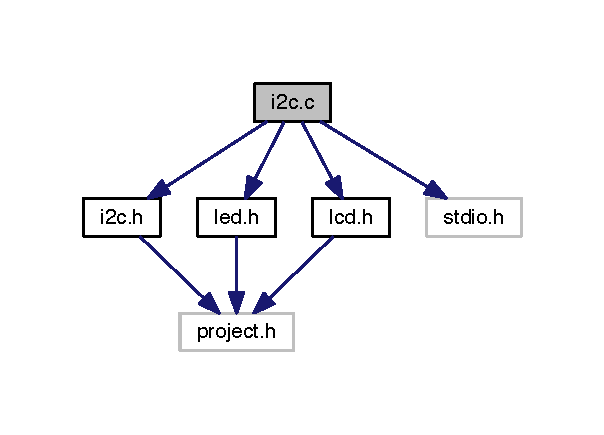
\includegraphics[width=350pt]{d6/d4e/i2c_8c__incl}
\end{center}
\end{figure}


\subsubsection{Detaljeret beskrivelse}
\hyperlink{class_i2_c}{I2C} modul. 

Håndter kommunikation via I2\+C-\/busset \begin{DoxyAuthor}{Forfatter}
Jeppe Stærk Antonsen (\href{mailto:201271201@uni.au.dk}{\tt 201271201@uni.\+au.\+dk}) 
\end{DoxyAuthor}

\hypertarget{i2c_8h}{}\subsection{i2c.\+h filreference}
\label{i2c_8h}\index{i2c.\+h@{i2c.\+h}}


\hyperlink{class_i2_c}{I2C} modul.  


{\ttfamily \#include $<$project.\+h$>$}\\*
Inklusions-\/afhængighedsgraf for i2c.\+h\+:\nopagebreak
\begin{figure}[H]
\begin{center}
\leavevmode
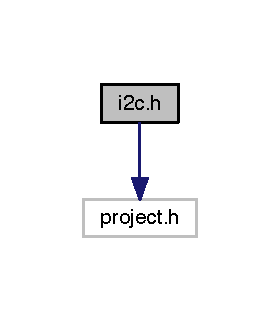
\includegraphics[width=134pt]{de/d0d/i2c_8h__incl}
\end{center}
\end{figure}
Denne graf viser, hvilke filer der direkte eller indirekte inkluderer denne fil\+:\nopagebreak
\begin{figure}[H]
\begin{center}
\leavevmode
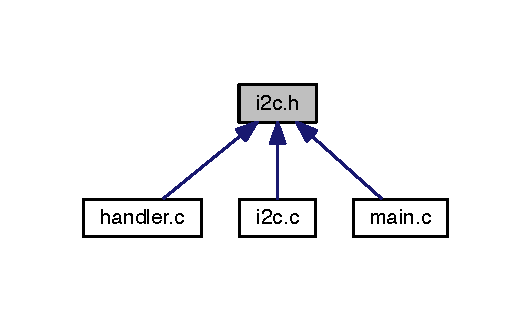
\includegraphics[width=255pt]{d3/df7/i2c_8h__dep__incl}
\end{center}
\end{figure}
\subsubsection*{\#Defines}
\begin{DoxyCompactItemize}
\item 
\#define \hyperlink{i2c_8h_a2c70db7df8defae29c1912d84aaee3dc}{P\+So\+C\+\_\+\+XY}~(0x08u)
\item 
\#define \hyperlink{i2c_8h_aa72315d85eb390444fdd96475c6aa1f4}{P\+So\+C\+\_\+Z}~(0x09u)
\item 
\#define \hyperlink{i2c_8h_adc44ca05813864518773ea6f3543816c}{P\+So\+C\+\_\+\+Sensor}~(0x10u)
\item 
\#define \hyperlink{i2c_8h_a6458dbf193a0eef0470fc1b08400bfcd}{I2\+C\+\_\+\+B\+U\+F\+F\+E\+R\+\_\+\+S\+I\+ZE}~(4u)
\item 
\#define \hyperlink{i2c_8h_a8c24abf58121f3c16b5f687cc2946cd1}{I2\+C\+\_\+\+P\+A\+C\+K\+E\+T\+\_\+\+S\+I\+ZE}~(4u)
\item 
\#define \hyperlink{i2c_8h_a1207f4b2c3692b1a344f0013da629310}{I2\+C\+\_\+\+P\+A\+C\+K\+E\+T\+\_\+\+S\+O\+P\+\_\+\+P\+OS}~(0u)
\item 
\#define \hyperlink{i2c_8h_ac13fcfeded7dc2d82fa4734456f3761f}{I2\+C\+\_\+\+P\+A\+C\+K\+E\+T\+\_\+\+C\+M\+D\+\_\+\+P\+OS}~(1u)
\item 
\#define \hyperlink{i2c_8h_a68506c3651f015716bb2c135e8e7b972}{I2\+C\+\_\+\+P\+A\+C\+K\+E\+T\+\_\+\+V\+A\+L\+\_\+\+P\+OS}~(2u)
\item 
\#define \hyperlink{i2c_8h_a940f0ea8103872c7ba81b9dc0f121feb}{I2\+C\+\_\+\+P\+A\+C\+K\+E\+T\+\_\+\+E\+O\+P\+\_\+\+P\+OS}~(3u)
\item 
\#define \hyperlink{i2c_8h_a52bb5b964361ed2f1b18df32c5b8f2c5}{I2\+C\+\_\+\+P\+A\+C\+K\+E\+T\+\_\+\+S\+OP}~(0x\+B\+Eu)
\item 
\#define \hyperlink{i2c_8h_a62b4ae6e51a3d0da47f5165165cdbc0a}{I2\+C\+\_\+\+P\+A\+C\+K\+E\+T\+\_\+\+E\+OP}~(0x\+E\+Fu)
\item 
\#define \hyperlink{i2c_8h_a7f8f53679384fa228bf06779cc168cfd}{I2\+C\+\_\+\+S\+T\+S\+\_\+\+C\+M\+D\+\_\+\+D\+O\+NE}~(0x\+A\+Au)
\item 
\#define \hyperlink{i2c_8h_aee0adbd7dcb13e95337369b7342a27e3}{I2\+C\+\_\+\+S\+T\+S\+\_\+\+C\+M\+D\+\_\+\+F\+A\+IL}~(0x\+E\+Eu)
\end{DoxyCompactItemize}
\subsubsection*{Funktioner}
\begin{DoxyCompactItemize}
\item 
void \hyperlink{i2c_8h_a5730d9445429351b9f750084c5cb5aae}{i2c\+\_\+init} (void)
\item 
void \hyperlink{i2c_8h_a0e13c9c7d87ebdb3680495a787f68d29}{i2c\+\_\+set\+Packet} (uint8 i2c\+Addr, uint8 i2c\+Cmd, uint8 i2c\+Val)
\item 
void \hyperlink{i2c_8h_afd44ef28b428b7ec2cffb38c97340251}{i2c\+\_\+get\+Packet} (uint8 i2c\+Addr, uint8 i2c\+Cmd, uint8 $\ast$i2c\+Val)
\end{DoxyCompactItemize}


\subsubsection{Detaljeret beskrivelse}
\hyperlink{class_i2_c}{I2C} modul. 

Håndter kommunikation via I2\+C-\/busset. \begin{DoxyAuthor}{Forfatter}
Jeppe Stærk Antonsen (\href{mailto:201271201@uni.au.dk}{\tt 201271201@uni.\+au.\+dk}) 
\end{DoxyAuthor}


\subsubsection{\#Define-\/dokumentation}
\index{i2c.\+h@{i2c.\+h}!I2\+C\+\_\+\+B\+U\+F\+F\+E\+R\+\_\+\+S\+I\+ZE@{I2\+C\+\_\+\+B\+U\+F\+F\+E\+R\+\_\+\+S\+I\+ZE}}
\index{I2\+C\+\_\+\+B\+U\+F\+F\+E\+R\+\_\+\+S\+I\+ZE@{I2\+C\+\_\+\+B\+U\+F\+F\+E\+R\+\_\+\+S\+I\+ZE}!i2c.\+h@{i2c.\+h}}
\paragraph[{\texorpdfstring{I2\+C\+\_\+\+B\+U\+F\+F\+E\+R\+\_\+\+S\+I\+ZE}{I2C_BUFFER_SIZE}}]{\setlength{\rightskip}{0pt plus 5cm}\#define I2\+C\+\_\+\+B\+U\+F\+F\+E\+R\+\_\+\+S\+I\+ZE~(4u)}\hypertarget{i2c_8h_a6458dbf193a0eef0470fc1b08400bfcd}{}\label{i2c_8h_a6458dbf193a0eef0470fc1b08400bfcd}


Defineret på linje 42 i filen i2c.\+h.



Refereret til af I2\+C\+::i2c\+\_\+rx() og I2\+C\+::i2c\+\_\+tx().

\index{i2c.\+h@{i2c.\+h}!I2\+C\+\_\+\+P\+A\+C\+K\+E\+T\+\_\+\+C\+M\+D\+\_\+\+P\+OS@{I2\+C\+\_\+\+P\+A\+C\+K\+E\+T\+\_\+\+C\+M\+D\+\_\+\+P\+OS}}
\index{I2\+C\+\_\+\+P\+A\+C\+K\+E\+T\+\_\+\+C\+M\+D\+\_\+\+P\+OS@{I2\+C\+\_\+\+P\+A\+C\+K\+E\+T\+\_\+\+C\+M\+D\+\_\+\+P\+OS}!i2c.\+h@{i2c.\+h}}
\paragraph[{\texorpdfstring{I2\+C\+\_\+\+P\+A\+C\+K\+E\+T\+\_\+\+C\+M\+D\+\_\+\+P\+OS}{I2C_PACKET_CMD_POS}}]{\setlength{\rightskip}{0pt plus 5cm}\#define I2\+C\+\_\+\+P\+A\+C\+K\+E\+T\+\_\+\+C\+M\+D\+\_\+\+P\+OS~(1u)}\hypertarget{i2c_8h_ac13fcfeded7dc2d82fa4734456f3761f}{}\label{i2c_8h_ac13fcfeded7dc2d82fa4734456f3761f}


Defineret på linje 47 i filen i2c.\+h.



Refereret til af I2\+C\+::i2c\+\_\+rx() og I2\+C\+::i2c\+\_\+tx().

\index{i2c.\+h@{i2c.\+h}!I2\+C\+\_\+\+P\+A\+C\+K\+E\+T\+\_\+\+E\+OP@{I2\+C\+\_\+\+P\+A\+C\+K\+E\+T\+\_\+\+E\+OP}}
\index{I2\+C\+\_\+\+P\+A\+C\+K\+E\+T\+\_\+\+E\+OP@{I2\+C\+\_\+\+P\+A\+C\+K\+E\+T\+\_\+\+E\+OP}!i2c.\+h@{i2c.\+h}}
\paragraph[{\texorpdfstring{I2\+C\+\_\+\+P\+A\+C\+K\+E\+T\+\_\+\+E\+OP}{I2C_PACKET_EOP}}]{\setlength{\rightskip}{0pt plus 5cm}\#define I2\+C\+\_\+\+P\+A\+C\+K\+E\+T\+\_\+\+E\+OP~(0x\+E\+Fu)}\hypertarget{i2c_8h_a62b4ae6e51a3d0da47f5165165cdbc0a}{}\label{i2c_8h_a62b4ae6e51a3d0da47f5165165cdbc0a}


Defineret på linje 53 i filen i2c.\+h.



Refereret til af I2\+C\+::i2c\+\_\+rx() og I2\+C\+::i2c\+\_\+tx().

\index{i2c.\+h@{i2c.\+h}!I2\+C\+\_\+\+P\+A\+C\+K\+E\+T\+\_\+\+E\+O\+P\+\_\+\+P\+OS@{I2\+C\+\_\+\+P\+A\+C\+K\+E\+T\+\_\+\+E\+O\+P\+\_\+\+P\+OS}}
\index{I2\+C\+\_\+\+P\+A\+C\+K\+E\+T\+\_\+\+E\+O\+P\+\_\+\+P\+OS@{I2\+C\+\_\+\+P\+A\+C\+K\+E\+T\+\_\+\+E\+O\+P\+\_\+\+P\+OS}!i2c.\+h@{i2c.\+h}}
\paragraph[{\texorpdfstring{I2\+C\+\_\+\+P\+A\+C\+K\+E\+T\+\_\+\+E\+O\+P\+\_\+\+P\+OS}{I2C_PACKET_EOP_POS}}]{\setlength{\rightskip}{0pt plus 5cm}\#define I2\+C\+\_\+\+P\+A\+C\+K\+E\+T\+\_\+\+E\+O\+P\+\_\+\+P\+OS~(3u)}\hypertarget{i2c_8h_a940f0ea8103872c7ba81b9dc0f121feb}{}\label{i2c_8h_a940f0ea8103872c7ba81b9dc0f121feb}


Defineret på linje 49 i filen i2c.\+h.



Refereret til af I2\+C\+::i2c\+\_\+rx() og I2\+C\+::i2c\+\_\+tx().

\index{i2c.\+h@{i2c.\+h}!I2\+C\+\_\+\+P\+A\+C\+K\+E\+T\+\_\+\+S\+I\+ZE@{I2\+C\+\_\+\+P\+A\+C\+K\+E\+T\+\_\+\+S\+I\+ZE}}
\index{I2\+C\+\_\+\+P\+A\+C\+K\+E\+T\+\_\+\+S\+I\+ZE@{I2\+C\+\_\+\+P\+A\+C\+K\+E\+T\+\_\+\+S\+I\+ZE}!i2c.\+h@{i2c.\+h}}
\paragraph[{\texorpdfstring{I2\+C\+\_\+\+P\+A\+C\+K\+E\+T\+\_\+\+S\+I\+ZE}{I2C_PACKET_SIZE}}]{\setlength{\rightskip}{0pt plus 5cm}\#define I2\+C\+\_\+\+P\+A\+C\+K\+E\+T\+\_\+\+S\+I\+ZE~(4u)}\hypertarget{i2c_8h_a8c24abf58121f3c16b5f687cc2946cd1}{}\label{i2c_8h_a8c24abf58121f3c16b5f687cc2946cd1}


Defineret på linje 43 i filen i2c.\+h.



Refereret til af I2\+C\+::i2c\+\_\+rx() og I2\+C\+::i2c\+\_\+tx().

\index{i2c.\+h@{i2c.\+h}!I2\+C\+\_\+\+P\+A\+C\+K\+E\+T\+\_\+\+S\+OP@{I2\+C\+\_\+\+P\+A\+C\+K\+E\+T\+\_\+\+S\+OP}}
\index{I2\+C\+\_\+\+P\+A\+C\+K\+E\+T\+\_\+\+S\+OP@{I2\+C\+\_\+\+P\+A\+C\+K\+E\+T\+\_\+\+S\+OP}!i2c.\+h@{i2c.\+h}}
\paragraph[{\texorpdfstring{I2\+C\+\_\+\+P\+A\+C\+K\+E\+T\+\_\+\+S\+OP}{I2C_PACKET_SOP}}]{\setlength{\rightskip}{0pt plus 5cm}\#define I2\+C\+\_\+\+P\+A\+C\+K\+E\+T\+\_\+\+S\+OP~(0x\+B\+Eu)}\hypertarget{i2c_8h_a52bb5b964361ed2f1b18df32c5b8f2c5}{}\label{i2c_8h_a52bb5b964361ed2f1b18df32c5b8f2c5}


Defineret på linje 52 i filen i2c.\+h.



Refereret til af I2\+C\+::i2c\+\_\+rx() og I2\+C\+::i2c\+\_\+tx().

\index{i2c.\+h@{i2c.\+h}!I2\+C\+\_\+\+P\+A\+C\+K\+E\+T\+\_\+\+S\+O\+P\+\_\+\+P\+OS@{I2\+C\+\_\+\+P\+A\+C\+K\+E\+T\+\_\+\+S\+O\+P\+\_\+\+P\+OS}}
\index{I2\+C\+\_\+\+P\+A\+C\+K\+E\+T\+\_\+\+S\+O\+P\+\_\+\+P\+OS@{I2\+C\+\_\+\+P\+A\+C\+K\+E\+T\+\_\+\+S\+O\+P\+\_\+\+P\+OS}!i2c.\+h@{i2c.\+h}}
\paragraph[{\texorpdfstring{I2\+C\+\_\+\+P\+A\+C\+K\+E\+T\+\_\+\+S\+O\+P\+\_\+\+P\+OS}{I2C_PACKET_SOP_POS}}]{\setlength{\rightskip}{0pt plus 5cm}\#define I2\+C\+\_\+\+P\+A\+C\+K\+E\+T\+\_\+\+S\+O\+P\+\_\+\+P\+OS~(0u)}\hypertarget{i2c_8h_a1207f4b2c3692b1a344f0013da629310}{}\label{i2c_8h_a1207f4b2c3692b1a344f0013da629310}


Defineret på linje 46 i filen i2c.\+h.



Refereret til af I2\+C\+::i2c\+\_\+rx() og I2\+C\+::i2c\+\_\+tx().

\index{i2c.\+h@{i2c.\+h}!I2\+C\+\_\+\+P\+A\+C\+K\+E\+T\+\_\+\+V\+A\+L\+\_\+\+P\+OS@{I2\+C\+\_\+\+P\+A\+C\+K\+E\+T\+\_\+\+V\+A\+L\+\_\+\+P\+OS}}
\index{I2\+C\+\_\+\+P\+A\+C\+K\+E\+T\+\_\+\+V\+A\+L\+\_\+\+P\+OS@{I2\+C\+\_\+\+P\+A\+C\+K\+E\+T\+\_\+\+V\+A\+L\+\_\+\+P\+OS}!i2c.\+h@{i2c.\+h}}
\paragraph[{\texorpdfstring{I2\+C\+\_\+\+P\+A\+C\+K\+E\+T\+\_\+\+V\+A\+L\+\_\+\+P\+OS}{I2C_PACKET_VAL_POS}}]{\setlength{\rightskip}{0pt plus 5cm}\#define I2\+C\+\_\+\+P\+A\+C\+K\+E\+T\+\_\+\+V\+A\+L\+\_\+\+P\+OS~(2u)}\hypertarget{i2c_8h_a68506c3651f015716bb2c135e8e7b972}{}\label{i2c_8h_a68506c3651f015716bb2c135e8e7b972}


Defineret på linje 48 i filen i2c.\+h.



Refereret til af I2\+C\+::i2c\+\_\+rx() og I2\+C\+::i2c\+\_\+tx().

\index{i2c.\+h@{i2c.\+h}!I2\+C\+\_\+\+S\+T\+S\+\_\+\+C\+M\+D\+\_\+\+D\+O\+NE@{I2\+C\+\_\+\+S\+T\+S\+\_\+\+C\+M\+D\+\_\+\+D\+O\+NE}}
\index{I2\+C\+\_\+\+S\+T\+S\+\_\+\+C\+M\+D\+\_\+\+D\+O\+NE@{I2\+C\+\_\+\+S\+T\+S\+\_\+\+C\+M\+D\+\_\+\+D\+O\+NE}!i2c.\+h@{i2c.\+h}}
\paragraph[{\texorpdfstring{I2\+C\+\_\+\+S\+T\+S\+\_\+\+C\+M\+D\+\_\+\+D\+O\+NE}{I2C_STS_CMD_DONE}}]{\setlength{\rightskip}{0pt plus 5cm}\#define I2\+C\+\_\+\+S\+T\+S\+\_\+\+C\+M\+D\+\_\+\+D\+O\+NE~(0x\+A\+Au)}\hypertarget{i2c_8h_a7f8f53679384fa228bf06779cc168cfd}{}\label{i2c_8h_a7f8f53679384fa228bf06779cc168cfd}


Defineret på linje 56 i filen i2c.\+h.



Refereret til af I2\+C\+::i2c\+\_\+get\+Packet(), I2\+C\+::i2c\+\_\+set\+Packet() og I2\+C\+::i2c\+\_\+tx().

\index{i2c.\+h@{i2c.\+h}!I2\+C\+\_\+\+S\+T\+S\+\_\+\+C\+M\+D\+\_\+\+F\+A\+IL@{I2\+C\+\_\+\+S\+T\+S\+\_\+\+C\+M\+D\+\_\+\+F\+A\+IL}}
\index{I2\+C\+\_\+\+S\+T\+S\+\_\+\+C\+M\+D\+\_\+\+F\+A\+IL@{I2\+C\+\_\+\+S\+T\+S\+\_\+\+C\+M\+D\+\_\+\+F\+A\+IL}!i2c.\+h@{i2c.\+h}}
\paragraph[{\texorpdfstring{I2\+C\+\_\+\+S\+T\+S\+\_\+\+C\+M\+D\+\_\+\+F\+A\+IL}{I2C_STS_CMD_FAIL}}]{\setlength{\rightskip}{0pt plus 5cm}\#define I2\+C\+\_\+\+S\+T\+S\+\_\+\+C\+M\+D\+\_\+\+F\+A\+IL~(0x\+E\+Eu)}\hypertarget{i2c_8h_aee0adbd7dcb13e95337369b7342a27e3}{}\label{i2c_8h_aee0adbd7dcb13e95337369b7342a27e3}


Defineret på linje 57 i filen i2c.\+h.



Refereret til af I2\+C\+::i2c\+\_\+rx() og I2\+C\+::i2c\+\_\+tx().

\index{i2c.\+h@{i2c.\+h}!P\+So\+C\+\_\+\+Sensor@{P\+So\+C\+\_\+\+Sensor}}
\index{P\+So\+C\+\_\+\+Sensor@{P\+So\+C\+\_\+\+Sensor}!i2c.\+h@{i2c.\+h}}
\paragraph[{\texorpdfstring{P\+So\+C\+\_\+\+Sensor}{PSoC_Sensor}}]{\setlength{\rightskip}{0pt plus 5cm}\#define P\+So\+C\+\_\+\+Sensor~(0x10u)}\hypertarget{i2c_8h_adc44ca05813864518773ea6f3543816c}{}\label{i2c_8h_adc44ca05813864518773ea6f3543816c}


Defineret på linje 39 i filen i2c.\+h.



Refereret til af Handler\+::handler().

\index{i2c.\+h@{i2c.\+h}!P\+So\+C\+\_\+\+XY@{P\+So\+C\+\_\+\+XY}}
\index{P\+So\+C\+\_\+\+XY@{P\+So\+C\+\_\+\+XY}!i2c.\+h@{i2c.\+h}}
\paragraph[{\texorpdfstring{P\+So\+C\+\_\+\+XY}{PSoC_XY}}]{\setlength{\rightskip}{0pt plus 5cm}\#define P\+So\+C\+\_\+\+XY~(0x08u)}\hypertarget{i2c_8h_a2c70db7df8defae29c1912d84aaee3dc}{}\label{i2c_8h_a2c70db7df8defae29c1912d84aaee3dc}


Defineret på linje 37 i filen i2c.\+h.



Refereret til af Handler\+::handler().

\index{i2c.\+h@{i2c.\+h}!P\+So\+C\+\_\+Z@{P\+So\+C\+\_\+Z}}
\index{P\+So\+C\+\_\+Z@{P\+So\+C\+\_\+Z}!i2c.\+h@{i2c.\+h}}
\paragraph[{\texorpdfstring{P\+So\+C\+\_\+Z}{PSoC_Z}}]{\setlength{\rightskip}{0pt plus 5cm}\#define P\+So\+C\+\_\+Z~(0x09u)}\hypertarget{i2c_8h_aa72315d85eb390444fdd96475c6aa1f4}{}\label{i2c_8h_aa72315d85eb390444fdd96475c6aa1f4}


Defineret på linje 38 i filen i2c.\+h.



Refereret til af Handler\+::handler().



\subsubsection{Funktions-\/dokumentation}
\index{i2c.\+h@{i2c.\+h}!i2c\+\_\+get\+Packet@{i2c\+\_\+get\+Packet}}
\index{i2c\+\_\+get\+Packet@{i2c\+\_\+get\+Packet}!i2c.\+h@{i2c.\+h}}
\paragraph[{\texorpdfstring{i2c\+\_\+get\+Packet(uint8 i2c\+Addr, uint8 i2c\+Cmd, uint8 $\ast$i2c\+Val)}{i2c_getPacket(uint8 i2cAddr, uint8 i2cCmd, uint8 *i2cVal)}}]{\setlength{\rightskip}{0pt plus 5cm}void i2c\+\_\+get\+Packet (
\begin{DoxyParamCaption}
\item[{uint8}]{i2c\+Addr, }
\item[{uint8}]{i2c\+Cmd, }
\item[{uint8 $\ast$}]{i2c\+Val}
\end{DoxyParamCaption}
)}\hypertarget{i2c_8h_afd44ef28b428b7ec2cffb38c97340251}{}\label{i2c_8h_afd44ef28b428b7ec2cffb38c97340251}
\index{i2c.\+h@{i2c.\+h}!i2c\+\_\+init@{i2c\+\_\+init}}
\index{i2c\+\_\+init@{i2c\+\_\+init}!i2c.\+h@{i2c.\+h}}
\paragraph[{\texorpdfstring{i2c\+\_\+init(void)}{i2c_init(void)}}]{\setlength{\rightskip}{0pt plus 5cm}void i2c\+\_\+init (
\begin{DoxyParamCaption}
\item[{void}]{}
\end{DoxyParamCaption}
)}\hypertarget{i2c_8h_a5730d9445429351b9f750084c5cb5aae}{}\label{i2c_8h_a5730d9445429351b9f750084c5cb5aae}
\index{i2c.\+h@{i2c.\+h}!i2c\+\_\+set\+Packet@{i2c\+\_\+set\+Packet}}
\index{i2c\+\_\+set\+Packet@{i2c\+\_\+set\+Packet}!i2c.\+h@{i2c.\+h}}
\paragraph[{\texorpdfstring{i2c\+\_\+set\+Packet(uint8 i2c\+Addr, uint8 i2c\+Cmd, uint8 i2c\+Val)}{i2c_setPacket(uint8 i2cAddr, uint8 i2cCmd, uint8 i2cVal)}}]{\setlength{\rightskip}{0pt plus 5cm}void i2c\+\_\+set\+Packet (
\begin{DoxyParamCaption}
\item[{uint8}]{i2c\+Addr, }
\item[{uint8}]{i2c\+Cmd, }
\item[{uint8}]{i2c\+Val}
\end{DoxyParamCaption}
)}\hypertarget{i2c_8h_a0e13c9c7d87ebdb3680495a787f68d29}{}\label{i2c_8h_a0e13c9c7d87ebdb3680495a787f68d29}

\hypertarget{lcd_8c}{}\subsection{lcd.\+c filreference}
\label{lcd_8c}\index{lcd.\+c@{lcd.\+c}}


\hyperlink{class_l_c_d}{L\+CD} modul.  


{\ttfamily \#include \char`\"{}data.\+h\char`\"{}}\\*
{\ttfamily \#include \char`\"{}Nokia5110\+L\+C\+D.\+h\char`\"{}}\\*
Inklusions-\/afhængighedsgraf for lcd.\+c\+:
\nopagebreak
\begin{figure}[H]
\begin{center}
\leavevmode
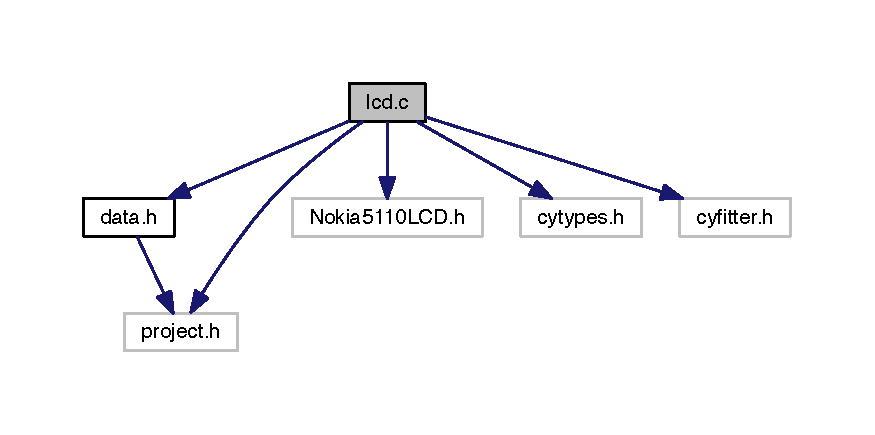
\includegraphics[width=350pt]{lcd_8c__incl}
\end{center}
\end{figure}


\subsubsection{Detaljeret beskrivelse}
\hyperlink{class_l_c_d}{L\+CD} modul. 

Sender tekst til Nokia5110\+L\+CD skærmen via dens eksterne kode. \begin{DoxyAuthor}{Forfatter}
Jeppe Stærk Antonsen (\href{mailto:201271201@uni.au.dk}{\tt 201271201@uni.\+au.\+dk}) 
\end{DoxyAuthor}

\hypertarget{lcd_8h}{}\subsection{lcd.\+h filreference}
\label{lcd_8h}\index{lcd.\+h@{lcd.\+h}}


\hyperlink{class_l_c_d}{L\+CD} modul.  


{\ttfamily \#include $<$project.\+h$>$}\\*
Inklusions-\/afhængighedsgraf for lcd.\+h\+:\nopagebreak
\begin{figure}[H]
\begin{center}
\leavevmode
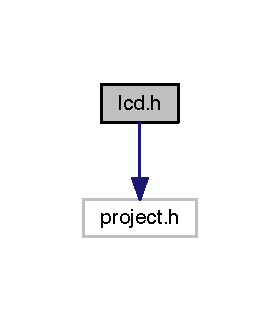
\includegraphics[width=134pt]{d7/d15/lcd_8h__incl}
\end{center}
\end{figure}
Denne graf viser, hvilke filer der direkte eller indirekte inkluderer denne fil\+:\nopagebreak
\begin{figure}[H]
\begin{center}
\leavevmode
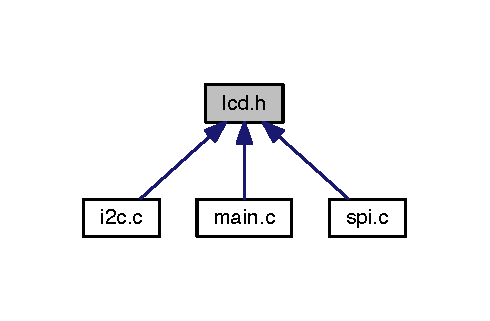
\includegraphics[width=235pt]{da/d0b/lcd_8h__dep__incl}
\end{center}
\end{figure}
\subsubsection*{Funktioner}
\begin{DoxyCompactItemize}
\item 
void \hyperlink{lcd_8h_a507dd352aee8161dc556e3d1439a2be2}{lcd\+\_\+newline} (char $\ast$characters)
\end{DoxyCompactItemize}


\subsubsection{Detaljeret beskrivelse}
\hyperlink{class_l_c_d}{L\+CD} modul. 

Sender tekst til Nokia5110\+L\+CD skærmen via dens eksterne kode. \begin{DoxyAuthor}{Forfatter}
Jeppe Stærk Antonsen (\href{mailto:201271201@uni.au.dk}{\tt 201271201@uni.\+au.\+dk}) 
\end{DoxyAuthor}


\subsubsection{Funktions-\/dokumentation}
\index{lcd.\+h@{lcd.\+h}!lcd\+\_\+newline@{lcd\+\_\+newline}}
\index{lcd\+\_\+newline@{lcd\+\_\+newline}!lcd.\+h@{lcd.\+h}}
\paragraph[{\texorpdfstring{lcd\+\_\+newline(char $\ast$characters)}{lcd_newline(char *characters)}}]{\setlength{\rightskip}{0pt plus 5cm}void lcd\+\_\+newline (
\begin{DoxyParamCaption}
\item[{char $\ast$}]{characters}
\end{DoxyParamCaption}
)}\hypertarget{lcd_8h_a507dd352aee8161dc556e3d1439a2be2}{}\label{lcd_8h_a507dd352aee8161dc556e3d1439a2be2}

\hypertarget{led_8c}{}\subsection{led.\+c filreference}
\label{led_8c}\index{led.\+c@{led.\+c}}


\hyperlink{class_l_e_d}{L\+ED} modul.  


{\ttfamily \#include \char`\"{}led.\+h\char`\"{}}\\*
Inklusions-\/afhængighedsgraf for led.\+c\+:\nopagebreak
\begin{figure}[H]
\begin{center}
\leavevmode
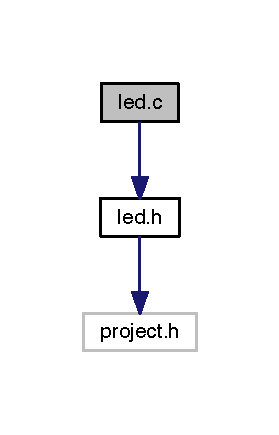
\includegraphics[width=134pt]{df/d0a/led_8c__incl}
\end{center}
\end{figure}


\subsubsection{Detaljeret beskrivelse}
\hyperlink{class_l_e_d}{L\+ED} modul. 

Håndtere P\+SoC\textquotesingle{}ens røde, grønne og blå led. \begin{DoxyAuthor}{Forfatter}
Casper Dieu Le (\href{mailto:201370338@uni.au.dk}{\tt 201370338@uni.\+au.\+dk}) 

Kasper Hinkler Uldbjerg (\href{mailto:201370281@uni.au.dk}{\tt 201370281@uni.\+au.\+dk}) 

Jeppe Stærk Antonsen (\href{mailto:201271201@uni.au.dk}{\tt 201271201@uni.\+au.\+dk}) 
\end{DoxyAuthor}

\hypertarget{led_8h}{}\subsection{led.\+h filreference}
\label{led_8h}\index{led.\+h@{led.\+h}}


\hyperlink{class_l_e_d}{L\+ED} modul.  


{\ttfamily \#include $<$project.\+h$>$}\\*
Inklusions-\/afhængighedsgraf for led.\+h\+:
\nopagebreak
\begin{figure}[H]
\begin{center}
\leavevmode
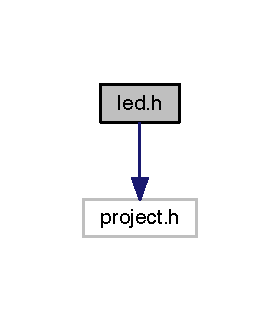
\includegraphics[width=134pt]{d6/d11/led_8h__incl}
\end{center}
\end{figure}
Denne graf viser, hvilke filer der direkte eller indirekte inkluderer denne fil\+:
\nopagebreak
\begin{figure}[H]
\begin{center}
\leavevmode
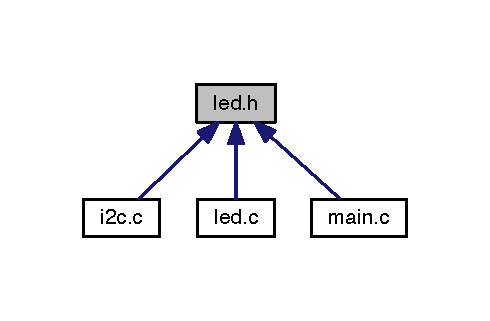
\includegraphics[width=235pt]{d6/dde/led_8h__dep__incl}
\end{center}
\end{figure}
\subsubsection*{\#Defines}
\begin{DoxyCompactItemize}
\item 
\#define \hyperlink{led_8h_af2e697ac60e05813d45ea2c9c9e79c25}{L\+E\+D\+\_\+\+ON}~(0u)
\item 
\#define \hyperlink{led_8h_a80700bb63bd56ebabbb4728aa433fd29}{L\+E\+D\+\_\+\+O\+FF}~(1u)
\end{DoxyCompactItemize}
\subsubsection*{Funktioner}
\begin{DoxyCompactItemize}
\item 
void \hyperlink{led_8h_a1d8e725e3829da99c1d027ba0a2ce57a}{set\+Led} (uint8 red, uint8 green, uint8 blue, uint8 delay)
\end{DoxyCompactItemize}


\subsubsection{Detaljeret beskrivelse}
\hyperlink{class_l_e_d}{L\+ED} modul. 

Håndtere P\+SoC\textquotesingle{}ens røde, grønne og blå led. \begin{DoxyAuthor}{Forfatter}
Jeppe Stærk Antonsen (\href{mailto:201271201@uni.au.dk}{\tt 201271201@uni.\+au.\+dk}) 
\end{DoxyAuthor}


\subsubsection{\#Define-\/dokumentation}
\index{led.\+h@{led.\+h}!L\+E\+D\+\_\+\+O\+FF@{L\+E\+D\+\_\+\+O\+FF}}
\index{L\+E\+D\+\_\+\+O\+FF@{L\+E\+D\+\_\+\+O\+FF}!led.\+h@{led.\+h}}
\paragraph[{\texorpdfstring{L\+E\+D\+\_\+\+O\+FF}{LED_OFF}}]{\setlength{\rightskip}{0pt plus 5cm}\#define L\+E\+D\+\_\+\+O\+FF~(1u)}\hypertarget{led_8h_a80700bb63bd56ebabbb4728aa433fd29}{}\label{led_8h_a80700bb63bd56ebabbb4728aa433fd29}


Defineret på linje 37 i filen led.\+h.



Refereret til af L\+E\+D\+::set\+Led().

\index{led.\+h@{led.\+h}!L\+E\+D\+\_\+\+ON@{L\+E\+D\+\_\+\+ON}}
\index{L\+E\+D\+\_\+\+ON@{L\+E\+D\+\_\+\+ON}!led.\+h@{led.\+h}}
\paragraph[{\texorpdfstring{L\+E\+D\+\_\+\+ON}{LED_ON}}]{\setlength{\rightskip}{0pt plus 5cm}\#define L\+E\+D\+\_\+\+ON~(0u)}\hypertarget{led_8h_af2e697ac60e05813d45ea2c9c9e79c25}{}\label{led_8h_af2e697ac60e05813d45ea2c9c9e79c25}


Defineret på linje 36 i filen led.\+h.



Refereret til af L\+E\+D\+::set\+Led().



\subsubsection{Funktions-\/dokumentation}
\index{led.\+h@{led.\+h}!set\+Led@{set\+Led}}
\index{set\+Led@{set\+Led}!led.\+h@{led.\+h}}
\paragraph[{\texorpdfstring{set\+Led(uint8 red, uint8 green, uint8 blue, uint8 delay)}{setLed(uint8 red, uint8 green, uint8 blue, uint8 delay)}}]{\setlength{\rightskip}{0pt plus 5cm}void set\+Led (
\begin{DoxyParamCaption}
\item[{uint8}]{red, }
\item[{uint8}]{green, }
\item[{uint8}]{blue, }
\item[{uint8}]{delay}
\end{DoxyParamCaption}
)}\hypertarget{led_8h_a1d8e725e3829da99c1d027ba0a2ce57a}{}\label{led_8h_a1d8e725e3829da99c1d027ba0a2ce57a}

\hypertarget{main_8c}{}\subsection{main.\+c filreference}
\label{main_8c}\index{main.\+c@{main.\+c}}


Hovedprogram.  


{\ttfamily \#include $<$project.\+h$>$}\\*
{\ttfamily \#include \char`\"{}data.\+h\char`\"{}}\\*
{\ttfamily \#include \char`\"{}handler.\+h\char`\"{}}\\*
{\ttfamily \#include \char`\"{}i2c.\+h\char`\"{}}\\*
{\ttfamily \#include \char`\"{}led.\+h\char`\"{}}\\*
{\ttfamily \#include \char`\"{}queue.\+h\char`\"{}}\\*
{\ttfamily \#include \char`\"{}xy.\+h\char`\"{}}\\*
Inklusions-\/afhængighedsgraf for main.\+c\+:
\nopagebreak
\begin{figure}[H]
\begin{center}
\leavevmode
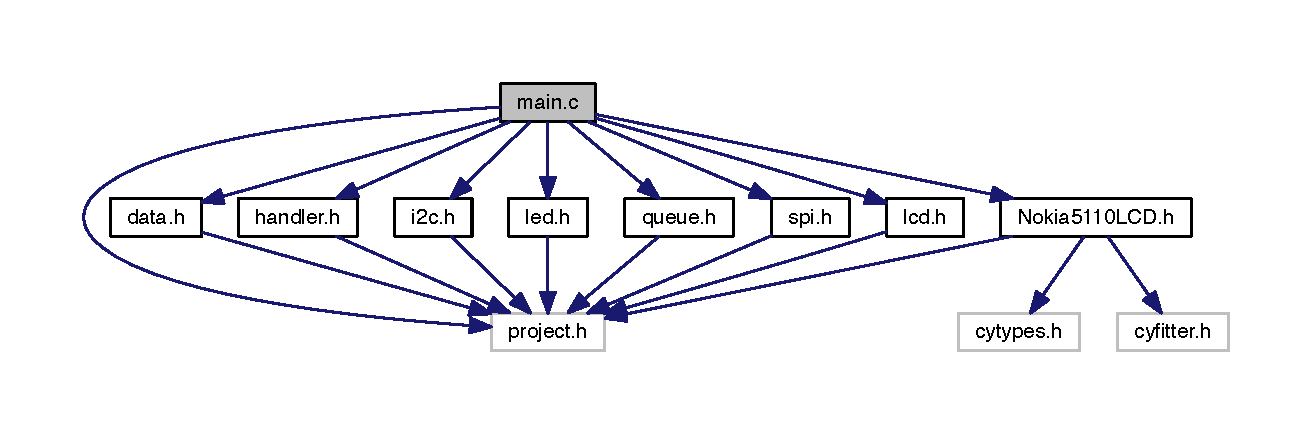
\includegraphics[width=350pt]{d4/d10/main_8c__incl}
\end{center}
\end{figure}
\subsubsection*{Funktioner}
\begin{DoxyCompactItemize}
\item 
int \hyperlink{main_8c_ae66f6b31b5ad750f1fe042a706a4e3d4}{main} ()
\end{DoxyCompactItemize}


\subsubsection{Detaljeret beskrivelse}
Hovedprogram. 

Intilizere modulerne og køre derefter i loop hvor der bliver kontrolieret om der er nogle actions i køen der skal håndteres af handleren. \begin{DoxyAuthor}{Forfatter}
Casper Dieu Le (\href{mailto:201370338@uni.au.dk}{\tt 201370338@uni.\+au.\+dk}) 

Kasper Hinkler Uldbjerg (\href{mailto:201370281@uni.au.dk}{\tt 201370281@uni.\+au.\+dk}) 

Jeppe Stærk (\href{mailto:201271201@uni.au.dk}{\tt 201271201@uni.\+au.\+dk}) 
\end{DoxyAuthor}


\subsubsection{Funktions-\/dokumentation}
\index{main.\+c@{main.\+c}!main@{main}}
\index{main@{main}!main.\+c@{main.\+c}}
\paragraph[{\texorpdfstring{main()}{main()}}]{\setlength{\rightskip}{0pt plus 5cm}int main (
\begin{DoxyParamCaption}
{}
\end{DoxyParamCaption}
)}\hypertarget{main_8c_ae66f6b31b5ad750f1fe042a706a4e3d4}{}\label{main_8c_ae66f6b31b5ad750f1fe042a706a4e3d4}


Defineret på linje 17 i filen main.\+c.



Indeholder referencer til X\+Y\+::calibrate\+X(), X\+Y\+::calibrate\+Y(), Data\+::data\+\_\+init(), Queue\+::front\+Queue(), Handler\+::handler(), I2\+C\+::i2c\+\_\+init(), I2\+C\+::i2c\+\_\+tx(), Queue\+::is\+Empty\+Queue(), Queue\+::pop\+Queue(), Queue\+::queue\+\_\+init(), L\+E\+D\+::set\+Led(), X\+Y\+::xy\+\_\+init() og X\+Y\+::xy\+\_\+start().


\begin{DoxyCode}
18 \{
19   CyGlobalIntEnable;
20   
21   \hyperlink{class_data_adf37c815716edf228a3cbb4564290275}{data\_init}();
22   \hyperlink{class_queue_a4e0a3758d721506e7729f4d074a280ff}{queue\_init}(6u);
23   \hyperlink{class_x_y_aaf6d50e1866014a76b1b15325d2dba4b}{xy\_init}();
24   \hyperlink{class_i2_c_a64303230bf4843297e7ac37ac236ca04}{i2c\_init}();
25   
26   DEBUG\_PutCRLF();
27   DEBUG\_PutString(\textcolor{stringliteral}{"===== Initializing PSoC XY ====="});
28   DEBUG\_PutCRLF();
29   
30   \hyperlink{class_l_e_d_a1d8e725e3829da99c1d027ba0a2ce57a}{setLed}(0,1,0,0);
31   CyDelay(100);
32   \hyperlink{class_l_e_d_a1d8e725e3829da99c1d027ba0a2ce57a}{setLed}(0,0,0,0);
33   
34   \hyperlink{class_x_y_a47c6cc7fae92395e4d1231428c7070d4}{xy\_start}();
35   
36   \textcolor{keywordflow}{for}(;;)
37   \{
38     \textcolor{keywordflow}{if}(SW2\_Read() == 0u)
39     \{
40       CyDelay(5u);
41       \textcolor{keywordflow}{if}(SW2\_Read() == 0u)
42       \{
43         \hyperlink{class_x_y_a852d7d757cec8e85e0b436969d0ce237}{calibrateX}();
44         \hyperlink{class_x_y_a86751f168bdc352fa109644298829609}{calibrateY}();
45       \}
46       \textcolor{keywordflow}{while}(SW2\_Read() == 0u)
47       \{
48         ; \textcolor{comment}{/* Wait till button released */}
49       \}
50     \}
51     
52     \textcolor{keywordflow}{while}(\hyperlink{class_queue_aafb324c79731abdc228dbf94d86722a3}{isEmptyQueue}() != 1)
53     \{
54       \textcolor{keyword}{struct }\hyperlink{queue_8h_df/d8c/struct_action}{Action} action;
55       action = \hyperlink{class_queue_a49c50ba30a42033068d8d8e6a23c6ca1}{frontQueue}();
56       \hyperlink{class_handler_af5be5b016b862943cd22504490acc8f4}{handler}(action.cmd, action.val);
57       \hyperlink{class_queue_a9ecab9ecdedfc331aed9a0ae63ce193b}{popQueue}();
58     \}
59     \hyperlink{class_i2_c_a3d3187ad377a6ca29b3fac5c809b6012}{i2c\_tx}();
60   \}
61 \}
\end{DoxyCode}


Her er kald-\/grafen for denne funktion\+:
\nopagebreak
\begin{figure}[H]
\begin{center}
\leavevmode
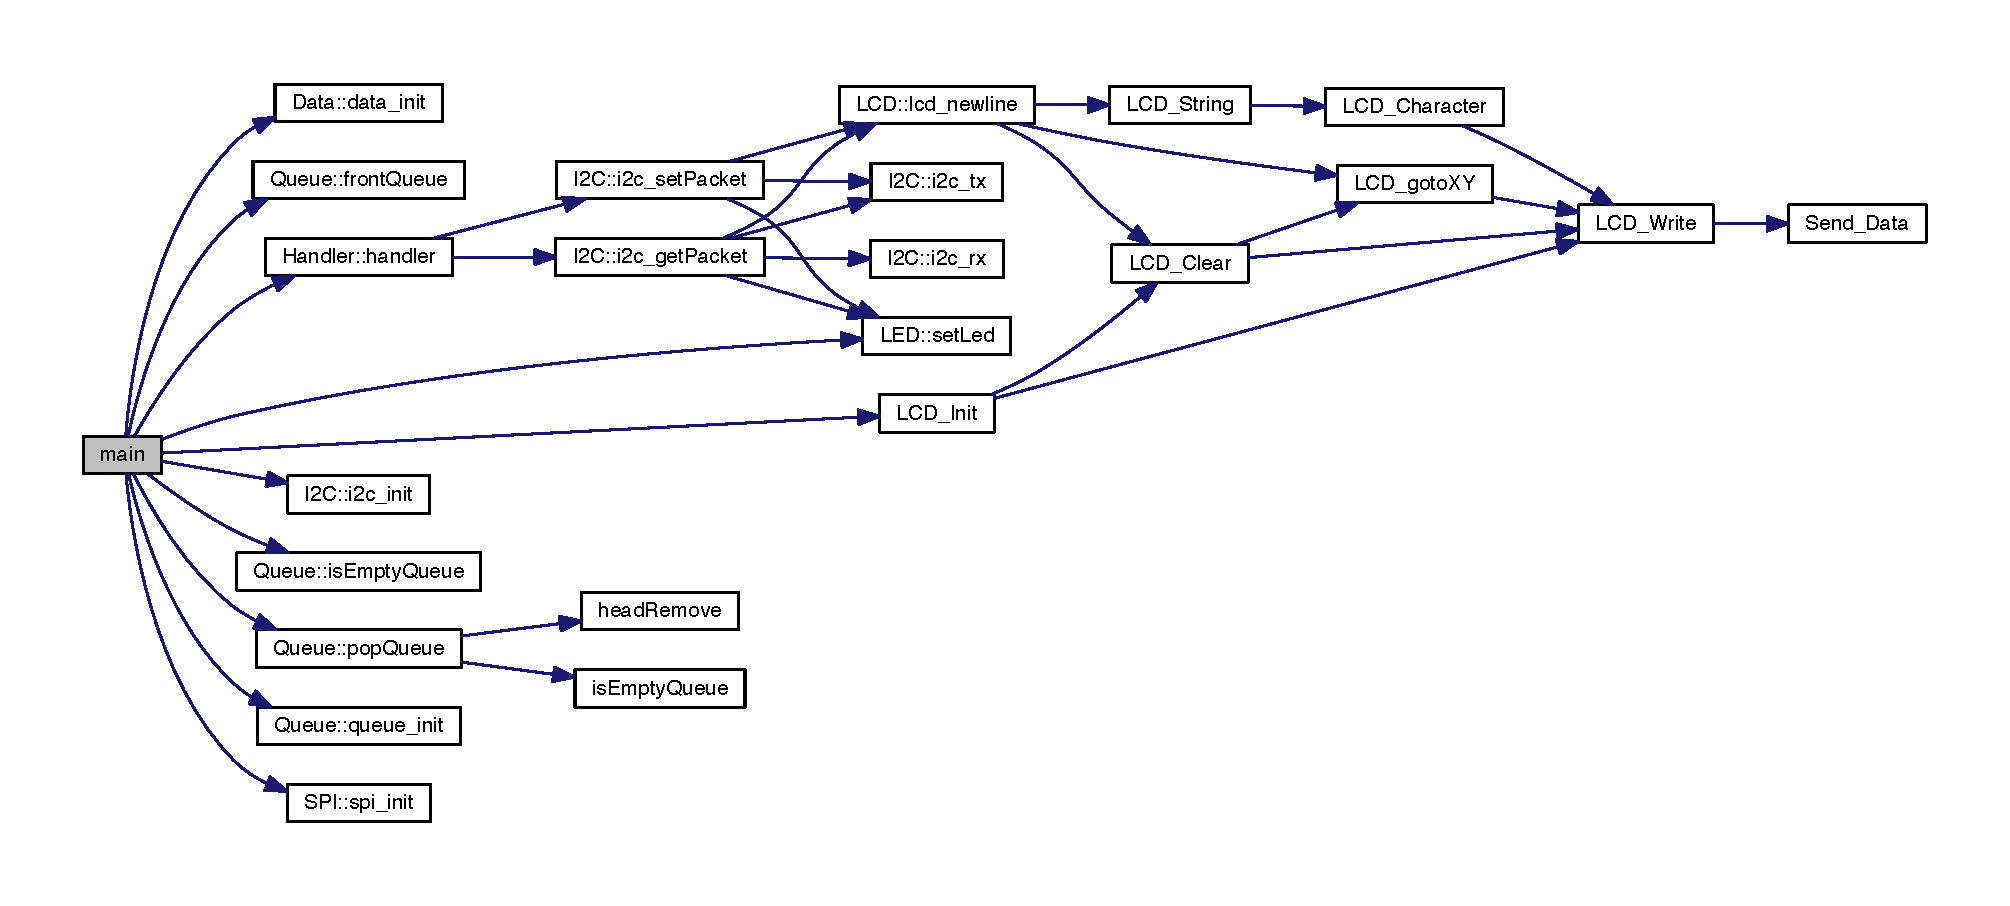
\includegraphics[width=350pt]{d0/d29/main_8c_ae66f6b31b5ad750f1fe042a706a4e3d4_cgraph}
\end{center}
\end{figure}



\hypertarget{_nokia5110_l_c_d_8c}{}\subsection{Nokia5110\+L\+C\+D.\+c filreference}
\label{_nokia5110_l_c_d_8c}\index{Nokia5110\+L\+C\+D.\+c@{Nokia5110\+L\+C\+D.\+c}}


Nokia5110\+L\+CD Modul (Impoteret)  


{\ttfamily \#include \char`\"{}Nokia5110\+L\+C\+D.\+h\char`\"{}}\\*
Inklusions-\/afhængighedsgraf for Nokia5110\+L\+C\+D.\+c\+:
\nopagebreak
\begin{figure}[H]
\begin{center}
\leavevmode
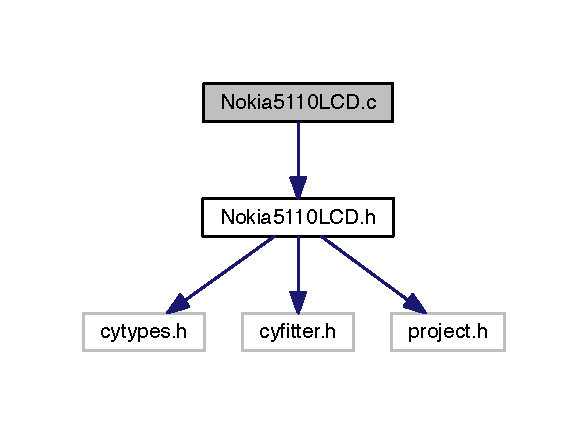
\includegraphics[width=282pt]{d6/de2/_nokia5110_l_c_d_8c__incl}
\end{center}
\end{figure}
\subsubsection*{Funktioner}
\begin{DoxyCompactItemize}
\item 
void \hyperlink{_nokia5110_l_c_d_8c_ae37cf16cd7f3298d819aede8023da757}{L\+C\+D\+\_\+\+Character} (uint8 character)
\item 
void \hyperlink{_nokia5110_l_c_d_8c_ae60d0b62d7eb3fa31266c095d7b3c245}{L\+C\+D\+\_\+\+Clear} (void)
\item 
void \hyperlink{_nokia5110_l_c_d_8c_aa53c9d40f3aa552a9974cd55ac510cb3}{L\+C\+D\+\_\+\+Init} (void)
\item 
void \hyperlink{_nokia5110_l_c_d_8c_a4c2c90307f23817e8445be5c6ca537c5}{L\+C\+D\+\_\+\+String} (char $\ast$characters)
\item 
void \hyperlink{_nokia5110_l_c_d_8c_aabeaad8714f6c1379e1d613e049554d1}{L\+C\+D\+\_\+\+Write} (uint8 data\+\_\+or\+\_\+command, uint8 data\+\_\+value)
\item 
void \hyperlink{_nokia5110_l_c_d_8c_ae1c81f642c55e721681c1049afc22e21}{Send\+\_\+\+Data} (int8 value)
\item 
void \hyperlink{_nokia5110_l_c_d_8c_adde1a4c2e7bd6bc1bbeb7694db45925b}{L\+C\+D\+\_\+goto\+XY} (uint8 x, uint8 y)
\item 
void \hyperlink{_nokia5110_l_c_d_8c_abcb278ab41675fe7ad44ff783e1d10ec}{L\+C\+D\+\_\+\+Bitmap} (char $\ast$my\+\_\+array)
\end{DoxyCompactItemize}
\subsubsection*{Variable}
\begin{DoxyCompactItemize}
\item 
static const uint8 \hyperlink{_nokia5110_l_c_d_8c_a15f4ad21eef7bd4012d7223cec9ec0dc}{Fonts} \mbox{[}$\,$\mbox{]}\mbox{[}\hyperlink{_nokia5110_l_c_d_8h_a7b2e9cc063e140c50b67a4f224988a45}{F\+O\+N\+T\+\_\+\+W\+I\+D\+TH}\mbox{]}
\item 
static const char \hyperlink{_nokia5110_l_c_d_8c_abd16123c1907b95492929b4e045c5bed}{Cypress\+Logo} \mbox{[}$\,$\mbox{]}
\end{DoxyCompactItemize}


\subsubsection{Detaljeret beskrivelse}
Nokia5110\+L\+CD Modul (Impoteret) 

Impoteret kildekode til Nokia 5110 L\+SD \begin{DoxyAuthor}{Forfatter}
Matt (cy.\+wbz) 
\end{DoxyAuthor}
\begin{DoxyRemark}{Bemærkninger}
\href{https://www.element14.com/community/thread/26122/l/psoc-4-pioneer-kit-community-project061-nokia-5110-lcd-interface?displayFullThread=true}{\tt https\+://www.\+element14.\+com/community/thread/26122/l/psoc-\/4-\/pioneer-\/kit-\/community-\/project061-\/nokia-\/5110-\/lcd-\/interface?display\+Full\+Thread=true} 
\end{DoxyRemark}


\subsubsection{Funktions-\/dokumentation}
\index{Nokia5110\+L\+C\+D.\+c@{Nokia5110\+L\+C\+D.\+c}!L\+C\+D\+\_\+\+Bitmap@{L\+C\+D\+\_\+\+Bitmap}}
\index{L\+C\+D\+\_\+\+Bitmap@{L\+C\+D\+\_\+\+Bitmap}!Nokia5110\+L\+C\+D.\+c@{Nokia5110\+L\+C\+D.\+c}}
\paragraph[{\texorpdfstring{L\+C\+D\+\_\+\+Bitmap(char $\ast$my\+\_\+array)}{LCD_Bitmap(char *my_array)}}]{\setlength{\rightskip}{0pt plus 5cm}void L\+C\+D\+\_\+\+Bitmap (
\begin{DoxyParamCaption}
\item[{char $\ast$}]{my\+\_\+array}
\end{DoxyParamCaption}
)}\hypertarget{_nokia5110_l_c_d_8c_abcb278ab41675fe7ad44ff783e1d10ec}{}\label{_nokia5110_l_c_d_8c_abcb278ab41675fe7ad44ff783e1d10ec}


Defineret på linje 396 i filen Nokia5110\+L\+C\+D.\+c.



Indeholder referencer til F\+O\+N\+T\+\_\+\+H\+E\+I\+G\+HT, L\+C\+D\+\_\+\+D\+A\+TA, L\+C\+D\+\_\+\+Write(), L\+C\+D\+\_\+X og L\+C\+D\+\_\+Y.


\begin{DoxyCode}
397 \{
398     uint16 index4;
399     \textcolor{keywordflow}{for} (index4 = 0 ; index4 < (\hyperlink{_nokia5110_l_c_d_8h_a808ffb5b80958b23f08910c0f38c53d3}{LCD\_X} * \hyperlink{_nokia5110_l_c_d_8h_ae5070c3ce78b96d41f8e166abff903ed}{LCD\_Y}/\hyperlink{_nokia5110_l_c_d_8h_a33f4fac49f2a5e27e2857eb27f054510}{FONT\_HEIGHT}) ; index4++)
400         
401         \textcolor{comment}{/* Take one byte at a time and send it to LCD as DATA */}
402         \hyperlink{_nokia5110_l_c_d_8c_aabeaad8714f6c1379e1d613e049554d1}{LCD\_Write}(\hyperlink{_nokia5110_l_c_d_8h_a25e9d818788f36ed74d7c4579f87f2a6}{LCD\_DATA}, my\_array[index4]);
403 \}
\end{DoxyCode}


Her er kald-\/grafen for denne funktion\+:
\nopagebreak
\begin{figure}[H]
\begin{center}
\leavevmode
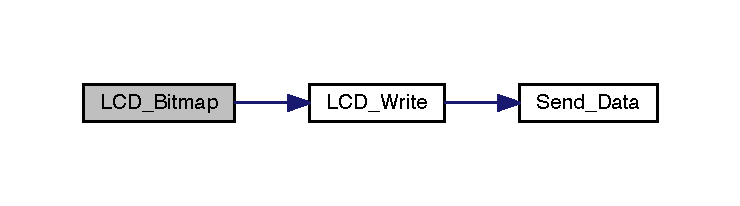
\includegraphics[width=350pt]{d7/dac/_nokia5110_l_c_d_8c_abcb278ab41675fe7ad44ff783e1d10ec_cgraph}
\end{center}
\end{figure}


\index{Nokia5110\+L\+C\+D.\+c@{Nokia5110\+L\+C\+D.\+c}!L\+C\+D\+\_\+\+Character@{L\+C\+D\+\_\+\+Character}}
\index{L\+C\+D\+\_\+\+Character@{L\+C\+D\+\_\+\+Character}!Nokia5110\+L\+C\+D.\+c@{Nokia5110\+L\+C\+D.\+c}}
\paragraph[{\texorpdfstring{L\+C\+D\+\_\+\+Character(uint8 character)}{LCD_Character(uint8 character)}}]{\setlength{\rightskip}{0pt plus 5cm}void L\+C\+D\+\_\+\+Character (
\begin{DoxyParamCaption}
\item[{uint8}]{character}
\end{DoxyParamCaption}
)}\hypertarget{_nokia5110_l_c_d_8c_ae37cf16cd7f3298d819aede8023da757}{}\label{_nokia5110_l_c_d_8c_ae37cf16cd7f3298d819aede8023da757}


Defineret på linje 167 i filen Nokia5110\+L\+C\+D.\+c.



Indeholder referencer til E\+M\+P\+T\+Y\+\_\+\+C\+O\+L\+U\+M\+N\+\_\+\+D\+A\+TA, F\+O\+N\+T\+\_\+\+W\+I\+D\+TH, Fonts, L\+C\+D\+\_\+\+D\+A\+TA, L\+C\+D\+\_\+\+Write() og O\+F\+F\+S\+E\+T\+\_\+\+F\+O\+R\+\_\+\+A\+S\+C\+II.



Refereret til af L\+C\+D\+\_\+\+String().


\begin{DoxyCode}
168 \{
169     uint16 index1;
170     \hyperlink{_nokia5110_l_c_d_8c_aabeaad8714f6c1379e1d613e049554d1}{LCD\_Write}(\hyperlink{_nokia5110_l_c_d_8h_a25e9d818788f36ed74d7c4579f87f2a6}{LCD\_DATA}, \hyperlink{_nokia5110_l_c_d_8h_aaafc5650777bddfbeabede2599523c79}{EMPTY\_COLUMN\_DATA});
171 
172     \textcolor{keywordflow}{for} (index1 = 0 ; index1 < \hyperlink{_nokia5110_l_c_d_8h_a7b2e9cc063e140c50b67a4f224988a45}{FONT\_WIDTH} ; index1++)
173         \hyperlink{_nokia5110_l_c_d_8c_aabeaad8714f6c1379e1d613e049554d1}{LCD\_Write}(\hyperlink{_nokia5110_l_c_d_8h_a25e9d818788f36ed74d7c4579f87f2a6}{LCD\_DATA}, \hyperlink{_nokia5110_l_c_d_8c_a15f4ad21eef7bd4012d7223cec9ec0dc}{Fonts}[character - 
      \hyperlink{_nokia5110_l_c_d_8h_a6252ed1db694fee526e93a1059e682d3}{OFFSET\_FOR\_ASCII}][index1]);
174 
175     \hyperlink{_nokia5110_l_c_d_8c_aabeaad8714f6c1379e1d613e049554d1}{LCD\_Write}(\hyperlink{_nokia5110_l_c_d_8h_a25e9d818788f36ed74d7c4579f87f2a6}{LCD\_DATA}, \hyperlink{_nokia5110_l_c_d_8h_aaafc5650777bddfbeabede2599523c79}{EMPTY\_COLUMN\_DATA});
176 \}
\end{DoxyCode}


Her er kald-\/grafen for denne funktion\+:
\nopagebreak
\begin{figure}[H]
\begin{center}
\leavevmode
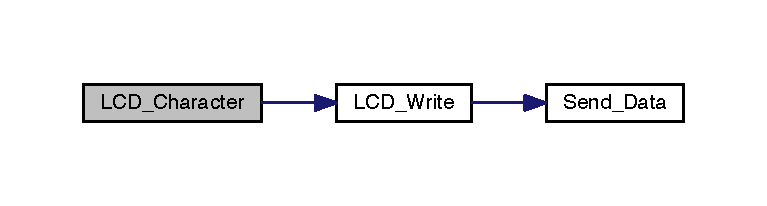
\includegraphics[width=350pt]{d7/dac/_nokia5110_l_c_d_8c_ae37cf16cd7f3298d819aede8023da757_cgraph}
\end{center}
\end{figure}




Her er kalder-\/grafen for denne funktion\+:
\nopagebreak
\begin{figure}[H]
\begin{center}
\leavevmode
\includegraphics[width=350pt]{d7/dac/_nokia5110_l_c_d_8c_ae37cf16cd7f3298d819aede8023da757_icgraph}
\end{center}
\end{figure}


\index{Nokia5110\+L\+C\+D.\+c@{Nokia5110\+L\+C\+D.\+c}!L\+C\+D\+\_\+\+Clear@{L\+C\+D\+\_\+\+Clear}}
\index{L\+C\+D\+\_\+\+Clear@{L\+C\+D\+\_\+\+Clear}!Nokia5110\+L\+C\+D.\+c@{Nokia5110\+L\+C\+D.\+c}}
\paragraph[{\texorpdfstring{L\+C\+D\+\_\+\+Clear(void)}{LCD_Clear(void)}}]{\setlength{\rightskip}{0pt plus 5cm}void L\+C\+D\+\_\+\+Clear (
\begin{DoxyParamCaption}
\item[{void}]{}
\end{DoxyParamCaption}
)}\hypertarget{_nokia5110_l_c_d_8c_ae60d0b62d7eb3fa31266c095d7b3c245}{}\label{_nokia5110_l_c_d_8c_ae60d0b62d7eb3fa31266c095d7b3c245}


Defineret på linje 193 i filen Nokia5110\+L\+C\+D.\+c.



Indeholder referencer til C\+O\+L\+U\+M\+N\+\_\+\+B\+E\+G\+I\+N\+N\+I\+NG, E\+M\+P\+T\+Y\+\_\+\+C\+O\+L\+U\+M\+N\+\_\+\+D\+A\+TA, F\+O\+N\+T\+\_\+\+H\+E\+I\+G\+HT, L\+C\+D\+\_\+\+D\+A\+TA, L\+C\+D\+\_\+goto\+X\+Y(), L\+C\+D\+\_\+\+Write(), L\+C\+D\+\_\+X, L\+C\+D\+\_\+Y og R\+O\+W\+\_\+\+B\+E\+G\+I\+N\+N\+I\+NG.



Refereret til af L\+C\+D\+\_\+\+Init() og L\+C\+D\+::lcd\+\_\+newline().


\begin{DoxyCode}
194 \{
195     uint16 index2;
196     \hyperlink{_nokia5110_l_c_d_8c_adde1a4c2e7bd6bc1bbeb7694db45925b}{LCD\_gotoXY}(\hyperlink{_nokia5110_l_c_d_8h_a36f758274dfeeb23c2494cd346144744}{COLUMN\_BEGINNING}, \hyperlink{_nokia5110_l_c_d_8h_a8b5d221d1489e603dd73680aad4bcdf8}{ROW\_BEGINNING});
197     
198     \textcolor{keywordflow}{for} (index2 = 0 ; index2 < (\hyperlink{_nokia5110_l_c_d_8h_a808ffb5b80958b23f08910c0f38c53d3}{LCD\_X} * \hyperlink{_nokia5110_l_c_d_8h_ae5070c3ce78b96d41f8e166abff903ed}{LCD\_Y}/\hyperlink{_nokia5110_l_c_d_8h_a33f4fac49f2a5e27e2857eb27f054510}{FONT\_HEIGHT}) ; index2++)
199         \hyperlink{_nokia5110_l_c_d_8c_aabeaad8714f6c1379e1d613e049554d1}{LCD\_Write}(\hyperlink{_nokia5110_l_c_d_8h_a25e9d818788f36ed74d7c4579f87f2a6}{LCD\_DATA}, \hyperlink{_nokia5110_l_c_d_8h_aaafc5650777bddfbeabede2599523c79}{EMPTY\_COLUMN\_DATA});
200         
201     \hyperlink{_nokia5110_l_c_d_8c_adde1a4c2e7bd6bc1bbeb7694db45925b}{LCD\_gotoXY}(\hyperlink{_nokia5110_l_c_d_8h_a36f758274dfeeb23c2494cd346144744}{COLUMN\_BEGINNING}, \hyperlink{_nokia5110_l_c_d_8h_a8b5d221d1489e603dd73680aad4bcdf8}{ROW\_BEGINNING});
202 \}
\end{DoxyCode}


Her er kald-\/grafen for denne funktion\+:
\nopagebreak
\begin{figure}[H]
\begin{center}
\leavevmode
\includegraphics[width=350pt]{d7/dac/_nokia5110_l_c_d_8c_ae60d0b62d7eb3fa31266c095d7b3c245_cgraph}
\end{center}
\end{figure}




Her er kalder-\/grafen for denne funktion\+:
\nopagebreak
\begin{figure}[H]
\begin{center}
\leavevmode
\includegraphics[width=350pt]{d7/dac/_nokia5110_l_c_d_8c_ae60d0b62d7eb3fa31266c095d7b3c245_icgraph}
\end{center}
\end{figure}


\index{Nokia5110\+L\+C\+D.\+c@{Nokia5110\+L\+C\+D.\+c}!L\+C\+D\+\_\+goto\+XY@{L\+C\+D\+\_\+goto\+XY}}
\index{L\+C\+D\+\_\+goto\+XY@{L\+C\+D\+\_\+goto\+XY}!Nokia5110\+L\+C\+D.\+c@{Nokia5110\+L\+C\+D.\+c}}
\paragraph[{\texorpdfstring{L\+C\+D\+\_\+goto\+X\+Y(uint8 x, uint8 y)}{LCD_gotoXY(uint8 x, uint8 y)}}]{\setlength{\rightskip}{0pt plus 5cm}void L\+C\+D\+\_\+goto\+XY (
\begin{DoxyParamCaption}
\item[{uint8}]{x, }
\item[{uint8}]{y}
\end{DoxyParamCaption}
)}\hypertarget{_nokia5110_l_c_d_8c_adde1a4c2e7bd6bc1bbeb7694db45925b}{}\label{_nokia5110_l_c_d_8c_adde1a4c2e7bd6bc1bbeb7694db45925b}


Defineret på linje 375 i filen Nokia5110\+L\+C\+D.\+c.



Indeholder referencer til C\+M\+D\+\_\+\+C\+O\+L\+U\+M\+N\+\_\+\+D\+A\+TA, C\+M\+D\+\_\+\+R\+O\+W\+\_\+\+D\+A\+TA, C\+O\+L\+U\+M\+N\+\_\+\+D\+A\+T\+A\+\_\+\+M\+A\+SK, L\+C\+D\+\_\+\+C\+O\+M\+M\+A\+ND, L\+C\+D\+\_\+\+Write() og R\+O\+W\+\_\+\+D\+A\+T\+A\+\_\+\+M\+A\+SK.



Refereret til af L\+C\+D\+\_\+\+Clear() og L\+C\+D\+::lcd\+\_\+newline().


\begin{DoxyCode}
376 \{
377     \hyperlink{_nokia5110_l_c_d_8c_aabeaad8714f6c1379e1d613e049554d1}{LCD\_Write}(\hyperlink{_nokia5110_l_c_d_8h_a11051095b0ca9f734b9e33117dac5ce8}{LCD\_COMMAND}, \hyperlink{_nokia5110_l_c_d_8h_a159a84674b38b66c1ea021331bdb757e}{CMD\_COLUMN\_DATA}  | (x & 
      \hyperlink{_nokia5110_l_c_d_8h_aba07c0bc26f47395b9daba931a5122e2}{COLUMN\_DATA\_MASK}));                       \textcolor{comment}{// Column}
378     \hyperlink{_nokia5110_l_c_d_8c_aabeaad8714f6c1379e1d613e049554d1}{LCD\_Write}(\hyperlink{_nokia5110_l_c_d_8h_a11051095b0ca9f734b9e33117dac5ce8}{LCD\_COMMAND}, \hyperlink{_nokia5110_l_c_d_8h_a9e25c527b4dd02cd409641483e2c9eb8}{CMD\_ROW\_DATA}     | (y & 
      \hyperlink{_nokia5110_l_c_d_8h_ab3d905cbccea22b6651d12b44d662e07}{ROW\_DATA\_MASK}));     \textcolor{comment}{// Row : Last 3 bits are valid}
379 \}
\end{DoxyCode}


Her er kald-\/grafen for denne funktion\+:
\nopagebreak
\begin{figure}[H]
\begin{center}
\leavevmode
\includegraphics[width=350pt]{d7/dac/_nokia5110_l_c_d_8c_adde1a4c2e7bd6bc1bbeb7694db45925b_cgraph}
\end{center}
\end{figure}




Her er kalder-\/grafen for denne funktion\+:
\nopagebreak
\begin{figure}[H]
\begin{center}
\leavevmode
\includegraphics[width=350pt]{d7/dac/_nokia5110_l_c_d_8c_adde1a4c2e7bd6bc1bbeb7694db45925b_icgraph}
\end{center}
\end{figure}


\index{Nokia5110\+L\+C\+D.\+c@{Nokia5110\+L\+C\+D.\+c}!L\+C\+D\+\_\+\+Init@{L\+C\+D\+\_\+\+Init}}
\index{L\+C\+D\+\_\+\+Init@{L\+C\+D\+\_\+\+Init}!Nokia5110\+L\+C\+D.\+c@{Nokia5110\+L\+C\+D.\+c}}
\paragraph[{\texorpdfstring{L\+C\+D\+\_\+\+Init(void)}{LCD_Init(void)}}]{\setlength{\rightskip}{0pt plus 5cm}void L\+C\+D\+\_\+\+Init (
\begin{DoxyParamCaption}
\item[{void}]{}
\end{DoxyParamCaption}
)}\hypertarget{_nokia5110_l_c_d_8c_aa53c9d40f3aa552a9974cd55ac510cb3}{}\label{_nokia5110_l_c_d_8c_aa53c9d40f3aa552a9974cd55ac510cb3}


Defineret på linje 220 i filen Nokia5110\+L\+C\+D.\+c.



Indeholder referencer til B\+I\+A\+S\+\_\+1\+\_\+\+B\+Y\+\_\+8, B\+I\+A\+S\+\_\+\+S\+Y\+S\+T\+E\+M\+\_\+\+M\+A\+SK, C\+M\+D\+\_\+\+B\+I\+A\+S\+\_\+\+S\+Y\+S\+T\+EM, C\+M\+D\+\_\+\+D\+I\+S\+P\+L\+A\+Y\+\_\+\+C\+O\+N\+T\+R\+OL, C\+M\+D\+\_\+\+F\+U\+N\+C\+T\+I\+O\+N\+\_\+\+S\+ET, C\+M\+D\+\_\+\+S\+E\+T\+\_\+\+V\+OP, C\+M\+D\+\_\+\+T\+E\+M\+P\+\_\+\+C\+O\+N\+T\+R\+OL, D\+E\+L\+A\+Y\+\_\+1\+\_\+\+MS, D\+I\+S\+P\+L\+A\+Y\+\_\+\+C\+O\+N\+T\+R\+O\+L\+\_\+\+M\+A\+SK, D\+I\+S\+P\+L\+A\+Y\+\_\+\+N\+O\+R\+M\+AL, F\+U\+N\+C\+T\+I\+O\+N\+\_\+\+S\+E\+T\+\_\+\+M\+A\+SK, H\+\_\+\+E\+X\+T\+E\+N\+D\+E\+D\+\_\+\+I\+N\+ST, H\+\_\+\+M\+A\+SK, H\+\_\+\+S\+H\+I\+FT, H\+I\+GH, L\+C\+D\+\_\+\+Clear(), L\+C\+D\+\_\+\+C\+O\+M\+M\+A\+ND, L\+C\+D\+\_\+\+Write(), L\+OW, P\+D\+\_\+\+C\+H\+I\+P\+\_\+\+A\+C\+T\+I\+VE, P\+D\+\_\+\+M\+A\+SK, P\+D\+\_\+\+S\+H\+I\+FT, S\+E\+T\+\_\+\+V\+O\+P\+\_\+5V, S\+E\+T\+\_\+\+V\+O\+P\+\_\+\+M\+A\+SK, T\+E\+M\+P\+\_\+\+C\+O\+N\+T\+R\+O\+L\+\_\+\+C\+O\+E\+F\+F0, T\+E\+M\+P\+\_\+\+C\+O\+N\+T\+R\+O\+L\+\_\+\+M\+A\+SK, V\+\_\+\+H\+O\+R\+I\+Z\+O\+N\+T\+A\+L\+\_\+\+A\+DD, V\+\_\+\+M\+A\+SK og V\+\_\+\+S\+H\+I\+FT.



Refereret til af main().


\begin{DoxyCode}
221 \{
222     \textcolor{comment}{/* Enable Gnd, Vcc & Backlight pins */}
223     Gnd\_Write(\hyperlink{_nokia5110_l_c_d_8h_ab811d8c6ff3a505312d3276590444289}{LOW});
224     Vcc\_Write(\hyperlink{_nokia5110_l_c_d_8h_a5bb885982ff66a2e0a0a45a8ee9c35e2}{HIGH});
225     BL\_Write(\hyperlink{_nokia5110_l_c_d_8h_a5bb885982ff66a2e0a0a45a8ee9c35e2}{HIGH});
226     
227     \textcolor{comment}{/* Reset the LCD - Active Low (1 -> 0 -> 1) */}
228     RST\_Write(\hyperlink{_nokia5110_l_c_d_8h_a5bb885982ff66a2e0a0a45a8ee9c35e2}{HIGH});
229     CyDelay(\hyperlink{_nokia5110_l_c_d_8h_a52bfdbdb0f66648736304dbed85b1eee}{DELAY\_1\_MS});
230     RST\_Write(\hyperlink{_nokia5110_l_c_d_8h_ab811d8c6ff3a505312d3276590444289}{LOW});
231     CyDelay(\hyperlink{_nokia5110_l_c_d_8h_a52bfdbdb0f66648736304dbed85b1eee}{DELAY\_1\_MS});
232     RST\_Write(\hyperlink{_nokia5110_l_c_d_8h_a5bb885982ff66a2e0a0a45a8ee9c35e2}{HIGH});
233     CyDelay(\hyperlink{_nokia5110_l_c_d_8h_a52bfdbdb0f66648736304dbed85b1eee}{DELAY\_1\_MS});
234     
235     \textcolor{comment}{/* No Power Down, Horizontal Addressing Mode, Extended Instruction set */}
236     \textcolor{comment}{/* 0x21 = 0010 0001    Instruction : Function Set (H=1)*/}
237     \hyperlink{_nokia5110_l_c_d_8c_aabeaad8714f6c1379e1d613e049554d1}{LCD\_Write}(\hyperlink{_nokia5110_l_c_d_8h_a11051095b0ca9f734b9e33117dac5ce8}{LCD\_COMMAND}, \hyperlink{_nokia5110_l_c_d_8h_a6e8374040226d7ea27d2783cae94f6ec}{CMD\_FUNCTION\_SET} | ((((
      \hyperlink{_nokia5110_l_c_d_8h_a8f280391129058891d6dafd25e9f5ebe}{PD\_CHIP\_ACTIVE} << \hyperlink{_nokia5110_l_c_d_8h_ab9126a4380117dcb422f1b2025a78cd1}{PD\_SHIFT}) & \hyperlink{_nokia5110_l_c_d_8h_ab44bdd714f3dcacacd2c8deca2f22568}{PD\_MASK}) \(\backslash\)
238     | ((\hyperlink{_nokia5110_l_c_d_8h_a28d9b8ca20803b32bfffb256a281404c}{V\_HORIZONTAL\_ADD} << \hyperlink{_nokia5110_l_c_d_8h_a634a68d0765064dec3171194ecb541b2}{V\_SHIFT}) & \hyperlink{_nokia5110_l_c_d_8h_a3964a8e86997d1704108bb308e5a644f}{V\_MASK}) | ((
      \hyperlink{_nokia5110_l_c_d_8h_aa22de21587e50b229df0eeb1fd90929c}{H\_EXTENDED\_INST} << \hyperlink{_nokia5110_l_c_d_8h_a2b197a68538e31c816ea8b8fa08b6d12}{H\_SHIFT}) & \hyperlink{_nokia5110_l_c_d_8h_a2c22a8118660a79c51b36ddf8f770f3b}{H\_MASK})) \(\backslash\)
239     & \hyperlink{_nokia5110_l_c_d_8h_a0203e2bfec43dd360d79d820f7e0da44}{FUNCTION\_SET\_MASK}));
240         
241     \textcolor{comment}{/* Set LCD Vop (Contrast): Try 0xB1(good @ 3.3V) or 0xBF if your display is too dark */}
242     \textcolor{comment}{/* 0xB1 = 1100 0000    Instruction : Set Vop */}
243     \hyperlink{_nokia5110_l_c_d_8c_aabeaad8714f6c1379e1d613e049554d1}{LCD\_Write}(\hyperlink{_nokia5110_l_c_d_8h_a11051095b0ca9f734b9e33117dac5ce8}{LCD\_COMMAND}, \hyperlink{_nokia5110_l_c_d_8h_a79bc3509563e0bac6c86290d41dcbdd8}{CMD\_SET\_VOP} | (
      \hyperlink{_nokia5110_l_c_d_8h_a0002e11f2ba33712a484e581f1991511}{SET\_VOP\_5V} & \hyperlink{_nokia5110_l_c_d_8h_aee5a1e57ccae6fbc08870442d754c787}{SET\_VOP\_MASK}));
244     
245     \textcolor{comment}{/* Set Temp coefficent */}
246     \textcolor{comment}{/* 0x04 = 0000 0100    Instruction : Temperature Control */}
247     \hyperlink{_nokia5110_l_c_d_8c_aabeaad8714f6c1379e1d613e049554d1}{LCD\_Write}(\hyperlink{_nokia5110_l_c_d_8h_a11051095b0ca9f734b9e33117dac5ce8}{LCD\_COMMAND}, \hyperlink{_nokia5110_l_c_d_8h_af5ea7845ce181a7511cace6bb548544a}{CMD\_TEMP\_CONTROL} | (
      \hyperlink{_nokia5110_l_c_d_8h_af9cffbe3b644b95e62af117cbe659acd}{TEMP\_CONTROL\_COEFF0} & \hyperlink{_nokia5110_l_c_d_8h_ad8dcbbb711cf2f05a28c0e702187ce35}{TEMP\_CONTROL\_MASK}));
248     
249     \textcolor{comment}{/* LCD bias mode 1:48: Try 0x13 or 0x14 */}
250     \textcolor{comment}{/* 0x13 = 0001 0100    Instruction : Bias System */}
251     \hyperlink{_nokia5110_l_c_d_8c_aabeaad8714f6c1379e1d613e049554d1}{LCD\_Write}(\hyperlink{_nokia5110_l_c_d_8h_a11051095b0ca9f734b9e33117dac5ce8}{LCD\_COMMAND}, \hyperlink{_nokia5110_l_c_d_8h_aa3b814f6b1578a9dbdeed06563f016b1}{CMD\_BIAS\_SYSTEM} | (
      \hyperlink{_nokia5110_l_c_d_8h_a5d9aa7fb016dea7e05a1de117ad0e4f5}{BIAS\_1\_BY\_8} & \hyperlink{_nokia5110_l_c_d_8h_a858abd2af474906b45154a5cc33add80}{BIAS\_SYSTEM\_MASK}));
252     
253     \textcolor{comment}{/* We must send 0x20 before modifying the display control mode */}
254     \textcolor{comment}{/* 0x20 = 0010 0000    Instruction : Function set (H=0)*/}
255     \hyperlink{_nokia5110_l_c_d_8c_aabeaad8714f6c1379e1d613e049554d1}{LCD\_Write}(\hyperlink{_nokia5110_l_c_d_8h_a11051095b0ca9f734b9e33117dac5ce8}{LCD\_COMMAND}, \hyperlink{_nokia5110_l_c_d_8h_a6e8374040226d7ea27d2783cae94f6ec}{CMD\_FUNCTION\_SET} | ((
      \hyperlink{_nokia5110_l_c_d_8h_a8f280391129058891d6dafd25e9f5ebe}{PD\_CHIP\_ACTIVE} << (\hyperlink{_nokia5110_l_c_d_8h_ab9126a4380117dcb422f1b2025a78cd1}{PD\_SHIFT} - 1)) & \hyperlink{_nokia5110_l_c_d_8h_a0203e2bfec43dd360d79d820f7e0da44}{FUNCTION\_SET\_MASK}));
256     
257     \textcolor{comment}{/* Set display control, normal mode. 0x0D for inverse */}
258     \textcolor{comment}{/* 0x0C = 0000 1101    Instruction : Display control */}
259     \hyperlink{_nokia5110_l_c_d_8c_aabeaad8714f6c1379e1d613e049554d1}{LCD\_Write}(\hyperlink{_nokia5110_l_c_d_8h_a11051095b0ca9f734b9e33117dac5ce8}{LCD\_COMMAND}, \hyperlink{_nokia5110_l_c_d_8h_a7cff120ed9b0fef8ea6e3c829155a6b7}{CMD\_DISPLAY\_CONTROL} | (
      \hyperlink{_nokia5110_l_c_d_8h_a28931614d96c39b23745dcf8e55001d7}{DISPLAY\_NORMAL} & \hyperlink{_nokia5110_l_c_d_8h_a2c15976b130befe754209d0379151982}{DISPLAY\_CONTROL\_MASK}));
260     
261     \textcolor{comment}{/* Clear the LCD screen */}
262     \hyperlink{_nokia5110_l_c_d_8c_ae60d0b62d7eb3fa31266c095d7b3c245}{LCD\_Clear}();
263     
264     \textcolor{comment}{/* Display bitmap image of Cypress Logo on the LCD */}
265 \textcolor{comment}{//    LCD\_Bitmap(CypressLogo);}
266     
267     \textcolor{comment}{/* Wait for 1 second before clearing the display */}
268 \textcolor{comment}{//    CyDelay(1000);}
269     
270     \hyperlink{_nokia5110_l_c_d_8c_ae60d0b62d7eb3fa31266c095d7b3c245}{LCD\_Clear}();
271 \}
\end{DoxyCode}


Her er kald-\/grafen for denne funktion\+:
\nopagebreak
\begin{figure}[H]
\begin{center}
\leavevmode
\includegraphics[width=350pt]{d7/dac/_nokia5110_l_c_d_8c_aa53c9d40f3aa552a9974cd55ac510cb3_cgraph}
\end{center}
\end{figure}




Her er kalder-\/grafen for denne funktion\+:
\nopagebreak
\begin{figure}[H]
\begin{center}
\leavevmode
\includegraphics[width=209pt]{d7/dac/_nokia5110_l_c_d_8c_aa53c9d40f3aa552a9974cd55ac510cb3_icgraph}
\end{center}
\end{figure}


\index{Nokia5110\+L\+C\+D.\+c@{Nokia5110\+L\+C\+D.\+c}!L\+C\+D\+\_\+\+String@{L\+C\+D\+\_\+\+String}}
\index{L\+C\+D\+\_\+\+String@{L\+C\+D\+\_\+\+String}!Nokia5110\+L\+C\+D.\+c@{Nokia5110\+L\+C\+D.\+c}}
\paragraph[{\texorpdfstring{L\+C\+D\+\_\+\+String(char $\ast$characters)}{LCD_String(char *characters)}}]{\setlength{\rightskip}{0pt plus 5cm}void L\+C\+D\+\_\+\+String (
\begin{DoxyParamCaption}
\item[{char $\ast$}]{characters}
\end{DoxyParamCaption}
)}\hypertarget{_nokia5110_l_c_d_8c_a4c2c90307f23817e8445be5c6ca537c5}{}\label{_nokia5110_l_c_d_8c_a4c2c90307f23817e8445be5c6ca537c5}


Defineret på linje 288 i filen Nokia5110\+L\+C\+D.\+c.



Indeholder referencer til L\+C\+D\+\_\+\+Character().



Refereret til af L\+C\+D\+::lcd\+\_\+newline().


\begin{DoxyCode}
289 \{
290     \textcolor{keywordflow}{while} (*characters)
291         \hyperlink{_nokia5110_l_c_d_8c_ae37cf16cd7f3298d819aede8023da757}{LCD\_Character}(*characters++);
292 \}
\end{DoxyCode}


Her er kald-\/grafen for denne funktion\+:
\nopagebreak
\begin{figure}[H]
\begin{center}
\leavevmode
\includegraphics[width=350pt]{d7/dac/_nokia5110_l_c_d_8c_a4c2c90307f23817e8445be5c6ca537c5_cgraph}
\end{center}
\end{figure}




Her er kalder-\/grafen for denne funktion\+:
\nopagebreak
\begin{figure}[H]
\begin{center}
\leavevmode
\includegraphics[width=350pt]{d7/dac/_nokia5110_l_c_d_8c_a4c2c90307f23817e8445be5c6ca537c5_icgraph}
\end{center}
\end{figure}


\index{Nokia5110\+L\+C\+D.\+c@{Nokia5110\+L\+C\+D.\+c}!L\+C\+D\+\_\+\+Write@{L\+C\+D\+\_\+\+Write}}
\index{L\+C\+D\+\_\+\+Write@{L\+C\+D\+\_\+\+Write}!Nokia5110\+L\+C\+D.\+c@{Nokia5110\+L\+C\+D.\+c}}
\paragraph[{\texorpdfstring{L\+C\+D\+\_\+\+Write(uint8 data\+\_\+or\+\_\+command, uint8 data\+\_\+value)}{LCD_Write(uint8 data_or_command, uint8 data_value)}}]{\setlength{\rightskip}{0pt plus 5cm}void L\+C\+D\+\_\+\+Write (
\begin{DoxyParamCaption}
\item[{uint8}]{data\+\_\+or\+\_\+command, }
\item[{uint8}]{data\+\_\+value}
\end{DoxyParamCaption}
)}\hypertarget{_nokia5110_l_c_d_8c_aabeaad8714f6c1379e1d613e049554d1}{}\label{_nokia5110_l_c_d_8c_aabeaad8714f6c1379e1d613e049554d1}


Defineret på linje 311 i filen Nokia5110\+L\+C\+D.\+c.



Indeholder referencer til D\+E\+L\+A\+Y\+\_\+1\+\_\+\+US, H\+I\+GH, L\+OW og Send\+\_\+\+Data().



Refereret til af L\+C\+D\+\_\+\+Bitmap(), L\+C\+D\+\_\+\+Character(), L\+C\+D\+\_\+\+Clear(), L\+C\+D\+\_\+goto\+X\+Y() og L\+C\+D\+\_\+\+Init().


\begin{DoxyCode}
312 \{
313     CE\_Write(\hyperlink{_nokia5110_l_c_d_8h_ab811d8c6ff3a505312d3276590444289}{LOW});
314     CyDelayUs(\hyperlink{_nokia5110_l_c_d_8h_ae3d7631de8f8bc443cfb910d8d7495ec}{DELAY\_1\_US});
315     DC\_Write(data\_or\_command);
316     \hyperlink{_nokia5110_l_c_d_8c_ae1c81f642c55e721681c1049afc22e21}{Send\_Data}(data\_value);
317     CE\_Write(\hyperlink{_nokia5110_l_c_d_8h_a5bb885982ff66a2e0a0a45a8ee9c35e2}{HIGH});
318     CyDelayUs(\hyperlink{_nokia5110_l_c_d_8h_ae3d7631de8f8bc443cfb910d8d7495ec}{DELAY\_1\_US});
319 \}
\end{DoxyCode}


Her er kald-\/grafen for denne funktion\+:
\nopagebreak
\begin{figure}[H]
\begin{center}
\leavevmode
\includegraphics[width=247pt]{d7/dac/_nokia5110_l_c_d_8c_aabeaad8714f6c1379e1d613e049554d1_cgraph}
\end{center}
\end{figure}




Her er kalder-\/grafen for denne funktion\+:
\nopagebreak
\begin{figure}[H]
\begin{center}
\leavevmode
\includegraphics[width=350pt]{d7/dac/_nokia5110_l_c_d_8c_aabeaad8714f6c1379e1d613e049554d1_icgraph}
\end{center}
\end{figure}


\index{Nokia5110\+L\+C\+D.\+c@{Nokia5110\+L\+C\+D.\+c}!Send\+\_\+\+Data@{Send\+\_\+\+Data}}
\index{Send\+\_\+\+Data@{Send\+\_\+\+Data}!Nokia5110\+L\+C\+D.\+c@{Nokia5110\+L\+C\+D.\+c}}
\paragraph[{\texorpdfstring{Send\+\_\+\+Data(int8 value)}{Send_Data(int8 value)}}]{\setlength{\rightskip}{0pt plus 5cm}void Send\+\_\+\+Data (
\begin{DoxyParamCaption}
\item[{int8}]{value}
\end{DoxyParamCaption}
)}\hypertarget{_nokia5110_l_c_d_8c_ae1c81f642c55e721681c1049afc22e21}{}\label{_nokia5110_l_c_d_8c_ae1c81f642c55e721681c1049afc22e21}


Defineret på linje 336 i filen Nokia5110\+L\+C\+D.\+c.



Indeholder referencer til D\+E\+L\+A\+Y\+\_\+1\+\_\+\+US, F\+O\+N\+T\+\_\+\+H\+E\+I\+G\+HT, H\+I\+GH, L\+OW, M\+Sb\+\_\+\+P\+O\+S\+I\+T\+I\+ON og S\+H\+I\+F\+T\+\_\+\+L\+E\+F\+T\+\_\+\+B\+Y\+\_\+1.



Refereret til af L\+C\+D\+\_\+\+Write().


\begin{DoxyCode}
337 \{
338     uint8 index3;
339     \textcolor{keywordflow}{for} (index3 = 0; index3 < \hyperlink{_nokia5110_l_c_d_8h_a33f4fac49f2a5e27e2857eb27f054510}{FONT\_HEIGHT}; index3++)
340     \{
341         \textcolor{comment}{/* Take one bit (MSb) at a time and send it to Data Input pin of LCD */}
342         \textcolor{keywordflow}{if}(\hyperlink{_nokia5110_l_c_d_8h_aef4c84e9494a5cb4f36b8f12b66d6dbd}{MSb\_POSITION} == (value & \hyperlink{_nokia5110_l_c_d_8h_aef4c84e9494a5cb4f36b8f12b66d6dbd}{MSb\_POSITION}))
343             Din\_Write(\hyperlink{_nokia5110_l_c_d_8h_a5bb885982ff66a2e0a0a45a8ee9c35e2}{HIGH});
344         \textcolor{keywordflow}{else}
345             Din\_Write(\hyperlink{_nokia5110_l_c_d_8h_ab811d8c6ff3a505312d3276590444289}{LOW});
346         
347         \textcolor{comment}{/* After setting the Data value on Din pin, toggle the Clock so that LCD can read Din */}
348         Clk\_Write(\hyperlink{_nokia5110_l_c_d_8h_a5bb885982ff66a2e0a0a45a8ee9c35e2}{HIGH});
349         CyDelayUs(\hyperlink{_nokia5110_l_c_d_8h_ae3d7631de8f8bc443cfb910d8d7495ec}{DELAY\_1\_US});
350         Clk\_Write(\hyperlink{_nokia5110_l_c_d_8h_ab811d8c6ff3a505312d3276590444289}{LOW});
351         CyDelayUs(\hyperlink{_nokia5110_l_c_d_8h_ae3d7631de8f8bc443cfb910d8d7495ec}{DELAY\_1\_US});
352         
353         \textcolor{comment}{/* Left shift the value before processing next bit */}
354         value <<= \hyperlink{_nokia5110_l_c_d_8h_af460569931827945c54504c0532bd91c}{SHIFT\_LEFT\_BY\_1};
355     \}
356 \}
\end{DoxyCode}


Her er kalder-\/grafen for denne funktion\+:
\nopagebreak
\begin{figure}[H]
\begin{center}
\leavevmode
\includegraphics[width=350pt]{d7/dac/_nokia5110_l_c_d_8c_ae1c81f642c55e721681c1049afc22e21_icgraph}
\end{center}
\end{figure}




\subsubsection{Variabel-\/dokumentation}
\index{Nokia5110\+L\+C\+D.\+c@{Nokia5110\+L\+C\+D.\+c}!Cypress\+Logo@{Cypress\+Logo}}
\index{Cypress\+Logo@{Cypress\+Logo}!Nokia5110\+L\+C\+D.\+c@{Nokia5110\+L\+C\+D.\+c}}
\paragraph[{\texorpdfstring{Cypress\+Logo}{CypressLogo}}]{\setlength{\rightskip}{0pt plus 5cm}const char Cypress\+Logo\mbox{[}$\,$\mbox{]}\hspace{0.3cm}{\ttfamily [static]}}\hypertarget{_nokia5110_l_c_d_8c_abd16123c1907b95492929b4e045c5bed}{}\label{_nokia5110_l_c_d_8c_abd16123c1907b95492929b4e045c5bed}


Defineret på linje 115 i filen Nokia5110\+L\+C\+D.\+c.

\index{Nokia5110\+L\+C\+D.\+c@{Nokia5110\+L\+C\+D.\+c}!Fonts@{Fonts}}
\index{Fonts@{Fonts}!Nokia5110\+L\+C\+D.\+c@{Nokia5110\+L\+C\+D.\+c}}
\paragraph[{\texorpdfstring{Fonts}{Fonts}}]{\setlength{\rightskip}{0pt plus 5cm}const uint8 Fonts\mbox{[}$\,$\mbox{]}\mbox{[}{\bf F\+O\+N\+T\+\_\+\+W\+I\+D\+TH}\mbox{]}\hspace{0.3cm}{\ttfamily [static]}}\hypertarget{_nokia5110_l_c_d_8c_a15f4ad21eef7bd4012d7223cec9ec0dc}{}\label{_nokia5110_l_c_d_8c_a15f4ad21eef7bd4012d7223cec9ec0dc}


Defineret på linje 14 i filen Nokia5110\+L\+C\+D.\+c.



Refereret til af L\+C\+D\+\_\+\+Character().


\hypertarget{_nokia5110_l_c_d_8h}{}\subsection{Nokia5110\+L\+C\+D.\+h filreference}
\label{_nokia5110_l_c_d_8h}\index{Nokia5110\+L\+C\+D.\+h@{Nokia5110\+L\+C\+D.\+h}}


Nokia5110\+L\+CD Modul (Impoteret)  


{\ttfamily \#include \char`\"{}cytypes.\+h\char`\"{}}\\*
{\ttfamily \#include \char`\"{}cyfitter.\+h\char`\"{}}\\*
{\ttfamily \#include \char`\"{}project.\+h\char`\"{}}\\*
Inklusions-\/afhængighedsgraf for Nokia5110\+L\+C\+D.\+h\+:
\nopagebreak
\begin{figure}[H]
\begin{center}
\leavevmode
\includegraphics[width=282pt]{d9/db8/_nokia5110_l_c_d_8h__incl}
\end{center}
\end{figure}
Denne graf viser, hvilke filer der direkte eller indirekte inkluderer denne fil\+:
\nopagebreak
\begin{figure}[H]
\begin{center}
\leavevmode
\includegraphics[width=289pt]{d7/d32/_nokia5110_l_c_d_8h__dep__incl}
\end{center}
\end{figure}
\subsubsection*{\#Defines}
\begin{DoxyCompactItemize}
\item 
\#define \hyperlink{_nokia5110_l_c_d_8h_a5bb885982ff66a2e0a0a45a8ee9c35e2}{H\+I\+GH}~1
\item 
\#define \hyperlink{_nokia5110_l_c_d_8h_ab811d8c6ff3a505312d3276590444289}{L\+OW}~0
\item 
\#define \hyperlink{_nokia5110_l_c_d_8h_a11051095b0ca9f734b9e33117dac5ce8}{L\+C\+D\+\_\+\+C\+O\+M\+M\+A\+ND}~\hyperlink{_nokia5110_l_c_d_8h_ab811d8c6ff3a505312d3276590444289}{L\+OW}
\item 
\#define \hyperlink{_nokia5110_l_c_d_8h_a25e9d818788f36ed74d7c4579f87f2a6}{L\+C\+D\+\_\+\+D\+A\+TA}~\hyperlink{_nokia5110_l_c_d_8h_a5bb885982ff66a2e0a0a45a8ee9c35e2}{H\+I\+GH}
\item 
\#define \hyperlink{_nokia5110_l_c_d_8h_a808ffb5b80958b23f08910c0f38c53d3}{L\+C\+D\+\_\+X}~84
\item 
\#define \hyperlink{_nokia5110_l_c_d_8h_ae5070c3ce78b96d41f8e166abff903ed}{L\+C\+D\+\_\+Y}~48
\item 
\#define \hyperlink{_nokia5110_l_c_d_8h_a33f4fac49f2a5e27e2857eb27f054510}{F\+O\+N\+T\+\_\+\+H\+E\+I\+G\+HT}~8
\item 
\#define \hyperlink{_nokia5110_l_c_d_8h_a7b2e9cc063e140c50b67a4f224988a45}{F\+O\+N\+T\+\_\+\+W\+I\+D\+TH}~5
\item 
\#define \hyperlink{_nokia5110_l_c_d_8h_aaafc5650777bddfbeabede2599523c79}{E\+M\+P\+T\+Y\+\_\+\+C\+O\+L\+U\+M\+N\+\_\+\+D\+A\+TA}~0x00u
\item 
\#define \hyperlink{_nokia5110_l_c_d_8h_a6252ed1db694fee526e93a1059e682d3}{O\+F\+F\+S\+E\+T\+\_\+\+F\+O\+R\+\_\+\+A\+S\+C\+II}~0x20u
\item 
\#define \hyperlink{_nokia5110_l_c_d_8h_aef4c84e9494a5cb4f36b8f12b66d6dbd}{M\+Sb\+\_\+\+P\+O\+S\+I\+T\+I\+ON}~0x80u
\item 
\#define \hyperlink{_nokia5110_l_c_d_8h_ae3d7631de8f8bc443cfb910d8d7495ec}{D\+E\+L\+A\+Y\+\_\+1\+\_\+\+US}~0x01u
\item 
\#define \hyperlink{_nokia5110_l_c_d_8h_a52bfdbdb0f66648736304dbed85b1eee}{D\+E\+L\+A\+Y\+\_\+1\+\_\+\+MS}~0x01u
\item 
\#define \hyperlink{_nokia5110_l_c_d_8h_a8b5d221d1489e603dd73680aad4bcdf8}{R\+O\+W\+\_\+\+B\+E\+G\+I\+N\+N\+I\+NG}~0x00u
\item 
\#define \hyperlink{_nokia5110_l_c_d_8h_a36f758274dfeeb23c2494cd346144744}{C\+O\+L\+U\+M\+N\+\_\+\+B\+E\+G\+I\+N\+N\+I\+NG}~0x00u
\item 
\#define \hyperlink{_nokia5110_l_c_d_8h_af460569931827945c54504c0532bd91c}{S\+H\+I\+F\+T\+\_\+\+L\+E\+F\+T\+\_\+\+B\+Y\+\_\+1}~0x01u
\item 
\#define \hyperlink{_nokia5110_l_c_d_8h_a6d864e31a00add16032f27b5e593b4bb}{C\+M\+D\+\_\+\+N\+OP}~0x00u
\item 
\#define \hyperlink{_nokia5110_l_c_d_8h_a6e8374040226d7ea27d2783cae94f6ec}{C\+M\+D\+\_\+\+F\+U\+N\+C\+T\+I\+O\+N\+\_\+\+S\+ET}~0x20u
\item 
\#define \hyperlink{_nokia5110_l_c_d_8h_a0203e2bfec43dd360d79d820f7e0da44}{F\+U\+N\+C\+T\+I\+O\+N\+\_\+\+S\+E\+T\+\_\+\+M\+A\+SK}~0x07u
\item 
\#define \hyperlink{_nokia5110_l_c_d_8h_ab9126a4380117dcb422f1b2025a78cd1}{P\+D\+\_\+\+S\+H\+I\+FT}~0x02u
\item 
\#define \hyperlink{_nokia5110_l_c_d_8h_ab44bdd714f3dcacacd2c8deca2f22568}{P\+D\+\_\+\+M\+A\+SK}~(0x01u $<$$<$ P\+D\+\_\+\+S\+H\+I\+F\+T)
\item 
\#define \hyperlink{_nokia5110_l_c_d_8h_a8f280391129058891d6dafd25e9f5ebe}{P\+D\+\_\+\+C\+H\+I\+P\+\_\+\+A\+C\+T\+I\+VE}~0x00u
\item 
\#define \hyperlink{_nokia5110_l_c_d_8h_a8ddbf58b86e22c415813a4ea9e764081}{P\+D\+\_\+\+C\+H\+I\+P\+\_\+\+P\+O\+W\+E\+R\+\_\+\+D\+O\+WN}~0x01u
\item 
\#define \hyperlink{_nokia5110_l_c_d_8h_a634a68d0765064dec3171194ecb541b2}{V\+\_\+\+S\+H\+I\+FT}~0x01u
\item 
\#define \hyperlink{_nokia5110_l_c_d_8h_a3964a8e86997d1704108bb308e5a644f}{V\+\_\+\+M\+A\+SK}~(0x01u $<$$<$ V\+\_\+\+S\+H\+I\+F\+T)
\item 
\#define \hyperlink{_nokia5110_l_c_d_8h_a28d9b8ca20803b32bfffb256a281404c}{V\+\_\+\+H\+O\+R\+I\+Z\+O\+N\+T\+A\+L\+\_\+\+A\+DD}~0x00u
\item 
\#define \hyperlink{_nokia5110_l_c_d_8h_a1a6ac64773c3262e04272091bf53821b}{V\+\_\+\+V\+E\+R\+T\+I\+C\+A\+L\+\_\+\+A\+DD}~0x01u
\item 
\#define \hyperlink{_nokia5110_l_c_d_8h_a2b197a68538e31c816ea8b8fa08b6d12}{H\+\_\+\+S\+H\+I\+FT}~0x00u
\item 
\#define \hyperlink{_nokia5110_l_c_d_8h_a2c22a8118660a79c51b36ddf8f770f3b}{H\+\_\+\+M\+A\+SK}~(0x01u $<$$<$ H\+\_\+\+S\+H\+I\+F\+T)
\item 
\#define \hyperlink{_nokia5110_l_c_d_8h_a8f90117fc14f59e334115f17181012cc}{H\+\_\+\+B\+A\+S\+I\+C\+\_\+\+I\+N\+ST}~0x00u
\item 
\#define \hyperlink{_nokia5110_l_c_d_8h_aa22de21587e50b229df0eeb1fd90929c}{H\+\_\+\+E\+X\+T\+E\+N\+D\+E\+D\+\_\+\+I\+N\+ST}~0x01u
\item 
\#define \hyperlink{_nokia5110_l_c_d_8h_a7cff120ed9b0fef8ea6e3c829155a6b7}{C\+M\+D\+\_\+\+D\+I\+S\+P\+L\+A\+Y\+\_\+\+C\+O\+N\+T\+R\+OL}~0x08u
\item 
\#define \hyperlink{_nokia5110_l_c_d_8h_a2c15976b130befe754209d0379151982}{D\+I\+S\+P\+L\+A\+Y\+\_\+\+C\+O\+N\+T\+R\+O\+L\+\_\+\+M\+A\+SK}~0x05u
\item 
\#define \hyperlink{_nokia5110_l_c_d_8h_a4fddc234feef030f001deedfd2ace43d}{D\+I\+S\+P\+L\+A\+Y\+\_\+\+B\+L\+A\+NK}~0x00u
\item 
\#define \hyperlink{_nokia5110_l_c_d_8h_a28931614d96c39b23745dcf8e55001d7}{D\+I\+S\+P\+L\+A\+Y\+\_\+\+N\+O\+R\+M\+AL}~0x04u
\item 
\#define \hyperlink{_nokia5110_l_c_d_8h_a00e2cdf2de65f1bcd39a7c489d41d7b1}{D\+I\+S\+P\+L\+A\+Y\+\_\+\+A\+L\+L\+\_\+\+S\+E\+G\+\_\+\+ON}~0x01u
\item 
\#define \hyperlink{_nokia5110_l_c_d_8h_a782cd7760554572a49711b9f87e49521}{D\+I\+S\+P\+L\+A\+Y\+\_\+\+I\+N\+V\+E\+R\+SE}~0x05u
\item 
\#define \hyperlink{_nokia5110_l_c_d_8h_a159a84674b38b66c1ea021331bdb757e}{C\+M\+D\+\_\+\+C\+O\+L\+U\+M\+N\+\_\+\+D\+A\+TA}~0x80u
\item 
\#define \hyperlink{_nokia5110_l_c_d_8h_aba07c0bc26f47395b9daba931a5122e2}{C\+O\+L\+U\+M\+N\+\_\+\+D\+A\+T\+A\+\_\+\+M\+A\+SK}~0x7\+Fu
\item 
\#define \hyperlink{_nokia5110_l_c_d_8h_a9e25c527b4dd02cd409641483e2c9eb8}{C\+M\+D\+\_\+\+R\+O\+W\+\_\+\+D\+A\+TA}~0x40u
\item 
\#define \hyperlink{_nokia5110_l_c_d_8h_ab3d905cbccea22b6651d12b44d662e07}{R\+O\+W\+\_\+\+D\+A\+T\+A\+\_\+\+M\+A\+SK}~0x07u
\item 
\#define \hyperlink{_nokia5110_l_c_d_8h_af5ea7845ce181a7511cace6bb548544a}{C\+M\+D\+\_\+\+T\+E\+M\+P\+\_\+\+C\+O\+N\+T\+R\+OL}~0x04u
\item 
\#define \hyperlink{_nokia5110_l_c_d_8h_ad8dcbbb711cf2f05a28c0e702187ce35}{T\+E\+M\+P\+\_\+\+C\+O\+N\+T\+R\+O\+L\+\_\+\+M\+A\+SK}~0x03u
\item 
\#define \hyperlink{_nokia5110_l_c_d_8h_af9cffbe3b644b95e62af117cbe659acd}{T\+E\+M\+P\+\_\+\+C\+O\+N\+T\+R\+O\+L\+\_\+\+C\+O\+E\+F\+F0}~0x00u
\item 
\#define \hyperlink{_nokia5110_l_c_d_8h_ab02971547e4e7ef6eb48acf0f24b5fcf}{T\+E\+M\+P\+\_\+\+C\+O\+N\+T\+R\+O\+L\+\_\+\+C\+O\+E\+F\+F1}~0x01u
\item 
\#define \hyperlink{_nokia5110_l_c_d_8h_ad212d2ee3db1b7e791f0ff4e4588d43c}{T\+E\+M\+P\+\_\+\+C\+O\+N\+T\+R\+O\+L\+\_\+\+C\+O\+E\+F\+F2}~0x02u
\item 
\#define \hyperlink{_nokia5110_l_c_d_8h_ac689369626c620c83a929c1591559249}{T\+E\+M\+P\+\_\+\+C\+O\+N\+T\+R\+O\+L\+\_\+\+C\+O\+E\+F\+F3}~0x03u
\item 
\#define \hyperlink{_nokia5110_l_c_d_8h_aa3b814f6b1578a9dbdeed06563f016b1}{C\+M\+D\+\_\+\+B\+I\+A\+S\+\_\+\+S\+Y\+S\+T\+EM}~0x10u
\item 
\#define \hyperlink{_nokia5110_l_c_d_8h_a858abd2af474906b45154a5cc33add80}{B\+I\+A\+S\+\_\+\+S\+Y\+S\+T\+E\+M\+\_\+\+M\+A\+SK}~0x07u
\item 
\#define \hyperlink{_nokia5110_l_c_d_8h_a9eedd99dcc0e312e70f5b6db0b4d312a}{B\+I\+A\+S\+\_\+1\+\_\+\+B\+Y\+\_\+11}~0x00u
\item 
\#define \hyperlink{_nokia5110_l_c_d_8h_af6af8ecd8604a8989a51509f52ad674e}{B\+I\+A\+S\+\_\+1\+\_\+\+B\+Y\+\_\+10}~0x01u
\item 
\#define \hyperlink{_nokia5110_l_c_d_8h_ae514d4e625e7d9f770372491de68b58e}{B\+I\+A\+S\+\_\+1\+\_\+\+B\+Y\+\_\+9}~0x02u
\item 
\#define \hyperlink{_nokia5110_l_c_d_8h_a5d9aa7fb016dea7e05a1de117ad0e4f5}{B\+I\+A\+S\+\_\+1\+\_\+\+B\+Y\+\_\+8}~0x03u
\item 
\#define \hyperlink{_nokia5110_l_c_d_8h_a9a8f397f23ef46cec53c8c8d8cf6749c}{B\+I\+A\+S\+\_\+1\+\_\+\+B\+Y\+\_\+7}~0x04u
\item 
\#define \hyperlink{_nokia5110_l_c_d_8h_af9a3cb3d794766d9ffd783022928c796}{B\+I\+A\+S\+\_\+1\+\_\+\+B\+Y\+\_\+6}~0x05u
\item 
\#define \hyperlink{_nokia5110_l_c_d_8h_a1afcdd109b8f8c22a442cc7d58d9f94e}{B\+I\+A\+S\+\_\+1\+\_\+\+B\+Y\+\_\+5}~0x06u
\item 
\#define \hyperlink{_nokia5110_l_c_d_8h_ac3603e4bb0eb123a928c510db3d7c6c9}{B\+I\+A\+S\+\_\+1\+\_\+\+B\+Y\+\_\+4}~0x07u
\item 
\#define \hyperlink{_nokia5110_l_c_d_8h_a79bc3509563e0bac6c86290d41dcbdd8}{C\+M\+D\+\_\+\+S\+E\+T\+\_\+\+V\+OP}~0x80u
\item 
\#define \hyperlink{_nokia5110_l_c_d_8h_aee5a1e57ccae6fbc08870442d754c787}{S\+E\+T\+\_\+\+V\+O\+P\+\_\+\+M\+A\+SK}~0x\+F\+Fu
\item 
\#define \hyperlink{_nokia5110_l_c_d_8h_a0002e11f2ba33712a484e581f1991511}{S\+E\+T\+\_\+\+V\+O\+P\+\_\+5V}~0x40u
\item 
\#define \hyperlink{_nokia5110_l_c_d_8h_ae5b0acd4304337f18d6d21dc03accde9}{S\+E\+T\+\_\+\+V\+O\+P\+\_\+3V}~0x31u
\end{DoxyCompactItemize}
\subsubsection*{Funktioner}
\begin{DoxyCompactItemize}
\item 
void \hyperlink{_nokia5110_l_c_d_8h_a71637602cbc84fdfc88fff1a96b97a75}{L\+C\+D\+\_\+\+Character} (uint8)
\item 
void \hyperlink{_nokia5110_l_c_d_8h_ae60d0b62d7eb3fa31266c095d7b3c245}{L\+C\+D\+\_\+\+Clear} (void)
\item 
void \hyperlink{_nokia5110_l_c_d_8h_aa53c9d40f3aa552a9974cd55ac510cb3}{L\+C\+D\+\_\+\+Init} (void)
\item 
void \hyperlink{_nokia5110_l_c_d_8h_a82777d8fcc63bb865a7df6be2e76ffc5}{L\+C\+D\+\_\+\+String} (char $\ast$)
\item 
void \hyperlink{_nokia5110_l_c_d_8h_a192f73998460ab575e8a8f07987c03a8}{L\+C\+D\+\_\+\+Write} (uint8, uint8)
\item 
void \hyperlink{_nokia5110_l_c_d_8h_a34baeac7ba9b692f9e18fbd65ecdfe4e}{Send\+\_\+\+Data} (int8)
\item 
void \hyperlink{_nokia5110_l_c_d_8h_ab28bb2063a03f0270671c8c3a27c01cc}{L\+C\+D\+\_\+goto\+XY} (uint8, uint8)
\item 
void \hyperlink{_nokia5110_l_c_d_8h_a55a5903f3473816bc2d74dd4e51047fc}{L\+C\+D\+\_\+\+Bitmap} (char $\ast$)
\end{DoxyCompactItemize}


\subsubsection{Detaljeret beskrivelse}
Nokia5110\+L\+CD Modul (Impoteret) 

Impoteret kildekode til Nokia 5110 L\+SD \begin{DoxyAuthor}{Forfatter}
Matt (cy.\+wbz) 
\end{DoxyAuthor}
\begin{DoxyRemark}{Bemærkninger}
\href{https://www.element14.com/community/thread/26122/l/psoc-4-pioneer-kit-community-project061-nokia-5110-lcd-interface?displayFullThread=true}{\tt https\+://www.\+element14.\+com/community/thread/26122/l/psoc-\/4-\/pioneer-\/kit-\/community-\/project061-\/nokia-\/5110-\/lcd-\/interface?display\+Full\+Thread=true} 
\end{DoxyRemark}


\subsubsection{\#Define-\/dokumentation}
\index{Nokia5110\+L\+C\+D.\+h@{Nokia5110\+L\+C\+D.\+h}!B\+I\+A\+S\+\_\+1\+\_\+\+B\+Y\+\_\+10@{B\+I\+A\+S\+\_\+1\+\_\+\+B\+Y\+\_\+10}}
\index{B\+I\+A\+S\+\_\+1\+\_\+\+B\+Y\+\_\+10@{B\+I\+A\+S\+\_\+1\+\_\+\+B\+Y\+\_\+10}!Nokia5110\+L\+C\+D.\+h@{Nokia5110\+L\+C\+D.\+h}}
\paragraph[{\texorpdfstring{B\+I\+A\+S\+\_\+1\+\_\+\+B\+Y\+\_\+10}{BIAS_1_BY_10}}]{\setlength{\rightskip}{0pt plus 5cm}\#define B\+I\+A\+S\+\_\+1\+\_\+\+B\+Y\+\_\+10~0x01u}\hypertarget{_nokia5110_l_c_d_8h_af6af8ecd8604a8989a51509f52ad674e}{}\label{_nokia5110_l_c_d_8h_af6af8ecd8604a8989a51509f52ad674e}


Defineret på linje 116 i filen Nokia5110\+L\+C\+D.\+h.

\index{Nokia5110\+L\+C\+D.\+h@{Nokia5110\+L\+C\+D.\+h}!B\+I\+A\+S\+\_\+1\+\_\+\+B\+Y\+\_\+11@{B\+I\+A\+S\+\_\+1\+\_\+\+B\+Y\+\_\+11}}
\index{B\+I\+A\+S\+\_\+1\+\_\+\+B\+Y\+\_\+11@{B\+I\+A\+S\+\_\+1\+\_\+\+B\+Y\+\_\+11}!Nokia5110\+L\+C\+D.\+h@{Nokia5110\+L\+C\+D.\+h}}
\paragraph[{\texorpdfstring{B\+I\+A\+S\+\_\+1\+\_\+\+B\+Y\+\_\+11}{BIAS_1_BY_11}}]{\setlength{\rightskip}{0pt plus 5cm}\#define B\+I\+A\+S\+\_\+1\+\_\+\+B\+Y\+\_\+11~0x00u}\hypertarget{_nokia5110_l_c_d_8h_a9eedd99dcc0e312e70f5b6db0b4d312a}{}\label{_nokia5110_l_c_d_8h_a9eedd99dcc0e312e70f5b6db0b4d312a}


Defineret på linje 115 i filen Nokia5110\+L\+C\+D.\+h.

\index{Nokia5110\+L\+C\+D.\+h@{Nokia5110\+L\+C\+D.\+h}!B\+I\+A\+S\+\_\+1\+\_\+\+B\+Y\+\_\+4@{B\+I\+A\+S\+\_\+1\+\_\+\+B\+Y\+\_\+4}}
\index{B\+I\+A\+S\+\_\+1\+\_\+\+B\+Y\+\_\+4@{B\+I\+A\+S\+\_\+1\+\_\+\+B\+Y\+\_\+4}!Nokia5110\+L\+C\+D.\+h@{Nokia5110\+L\+C\+D.\+h}}
\paragraph[{\texorpdfstring{B\+I\+A\+S\+\_\+1\+\_\+\+B\+Y\+\_\+4}{BIAS_1_BY_4}}]{\setlength{\rightskip}{0pt plus 5cm}\#define B\+I\+A\+S\+\_\+1\+\_\+\+B\+Y\+\_\+4~0x07u}\hypertarget{_nokia5110_l_c_d_8h_ac3603e4bb0eb123a928c510db3d7c6c9}{}\label{_nokia5110_l_c_d_8h_ac3603e4bb0eb123a928c510db3d7c6c9}


Defineret på linje 122 i filen Nokia5110\+L\+C\+D.\+h.

\index{Nokia5110\+L\+C\+D.\+h@{Nokia5110\+L\+C\+D.\+h}!B\+I\+A\+S\+\_\+1\+\_\+\+B\+Y\+\_\+5@{B\+I\+A\+S\+\_\+1\+\_\+\+B\+Y\+\_\+5}}
\index{B\+I\+A\+S\+\_\+1\+\_\+\+B\+Y\+\_\+5@{B\+I\+A\+S\+\_\+1\+\_\+\+B\+Y\+\_\+5}!Nokia5110\+L\+C\+D.\+h@{Nokia5110\+L\+C\+D.\+h}}
\paragraph[{\texorpdfstring{B\+I\+A\+S\+\_\+1\+\_\+\+B\+Y\+\_\+5}{BIAS_1_BY_5}}]{\setlength{\rightskip}{0pt plus 5cm}\#define B\+I\+A\+S\+\_\+1\+\_\+\+B\+Y\+\_\+5~0x06u}\hypertarget{_nokia5110_l_c_d_8h_a1afcdd109b8f8c22a442cc7d58d9f94e}{}\label{_nokia5110_l_c_d_8h_a1afcdd109b8f8c22a442cc7d58d9f94e}


Defineret på linje 121 i filen Nokia5110\+L\+C\+D.\+h.

\index{Nokia5110\+L\+C\+D.\+h@{Nokia5110\+L\+C\+D.\+h}!B\+I\+A\+S\+\_\+1\+\_\+\+B\+Y\+\_\+6@{B\+I\+A\+S\+\_\+1\+\_\+\+B\+Y\+\_\+6}}
\index{B\+I\+A\+S\+\_\+1\+\_\+\+B\+Y\+\_\+6@{B\+I\+A\+S\+\_\+1\+\_\+\+B\+Y\+\_\+6}!Nokia5110\+L\+C\+D.\+h@{Nokia5110\+L\+C\+D.\+h}}
\paragraph[{\texorpdfstring{B\+I\+A\+S\+\_\+1\+\_\+\+B\+Y\+\_\+6}{BIAS_1_BY_6}}]{\setlength{\rightskip}{0pt plus 5cm}\#define B\+I\+A\+S\+\_\+1\+\_\+\+B\+Y\+\_\+6~0x05u}\hypertarget{_nokia5110_l_c_d_8h_af9a3cb3d794766d9ffd783022928c796}{}\label{_nokia5110_l_c_d_8h_af9a3cb3d794766d9ffd783022928c796}


Defineret på linje 120 i filen Nokia5110\+L\+C\+D.\+h.

\index{Nokia5110\+L\+C\+D.\+h@{Nokia5110\+L\+C\+D.\+h}!B\+I\+A\+S\+\_\+1\+\_\+\+B\+Y\+\_\+7@{B\+I\+A\+S\+\_\+1\+\_\+\+B\+Y\+\_\+7}}
\index{B\+I\+A\+S\+\_\+1\+\_\+\+B\+Y\+\_\+7@{B\+I\+A\+S\+\_\+1\+\_\+\+B\+Y\+\_\+7}!Nokia5110\+L\+C\+D.\+h@{Nokia5110\+L\+C\+D.\+h}}
\paragraph[{\texorpdfstring{B\+I\+A\+S\+\_\+1\+\_\+\+B\+Y\+\_\+7}{BIAS_1_BY_7}}]{\setlength{\rightskip}{0pt plus 5cm}\#define B\+I\+A\+S\+\_\+1\+\_\+\+B\+Y\+\_\+7~0x04u}\hypertarget{_nokia5110_l_c_d_8h_a9a8f397f23ef46cec53c8c8d8cf6749c}{}\label{_nokia5110_l_c_d_8h_a9a8f397f23ef46cec53c8c8d8cf6749c}


Defineret på linje 119 i filen Nokia5110\+L\+C\+D.\+h.

\index{Nokia5110\+L\+C\+D.\+h@{Nokia5110\+L\+C\+D.\+h}!B\+I\+A\+S\+\_\+1\+\_\+\+B\+Y\+\_\+8@{B\+I\+A\+S\+\_\+1\+\_\+\+B\+Y\+\_\+8}}
\index{B\+I\+A\+S\+\_\+1\+\_\+\+B\+Y\+\_\+8@{B\+I\+A\+S\+\_\+1\+\_\+\+B\+Y\+\_\+8}!Nokia5110\+L\+C\+D.\+h@{Nokia5110\+L\+C\+D.\+h}}
\paragraph[{\texorpdfstring{B\+I\+A\+S\+\_\+1\+\_\+\+B\+Y\+\_\+8}{BIAS_1_BY_8}}]{\setlength{\rightskip}{0pt plus 5cm}\#define B\+I\+A\+S\+\_\+1\+\_\+\+B\+Y\+\_\+8~0x03u}\hypertarget{_nokia5110_l_c_d_8h_a5d9aa7fb016dea7e05a1de117ad0e4f5}{}\label{_nokia5110_l_c_d_8h_a5d9aa7fb016dea7e05a1de117ad0e4f5}


Defineret på linje 118 i filen Nokia5110\+L\+C\+D.\+h.



Refereret til af L\+C\+D\+\_\+\+Init().

\index{Nokia5110\+L\+C\+D.\+h@{Nokia5110\+L\+C\+D.\+h}!B\+I\+A\+S\+\_\+1\+\_\+\+B\+Y\+\_\+9@{B\+I\+A\+S\+\_\+1\+\_\+\+B\+Y\+\_\+9}}
\index{B\+I\+A\+S\+\_\+1\+\_\+\+B\+Y\+\_\+9@{B\+I\+A\+S\+\_\+1\+\_\+\+B\+Y\+\_\+9}!Nokia5110\+L\+C\+D.\+h@{Nokia5110\+L\+C\+D.\+h}}
\paragraph[{\texorpdfstring{B\+I\+A\+S\+\_\+1\+\_\+\+B\+Y\+\_\+9}{BIAS_1_BY_9}}]{\setlength{\rightskip}{0pt plus 5cm}\#define B\+I\+A\+S\+\_\+1\+\_\+\+B\+Y\+\_\+9~0x02u}\hypertarget{_nokia5110_l_c_d_8h_ae514d4e625e7d9f770372491de68b58e}{}\label{_nokia5110_l_c_d_8h_ae514d4e625e7d9f770372491de68b58e}


Defineret på linje 117 i filen Nokia5110\+L\+C\+D.\+h.

\index{Nokia5110\+L\+C\+D.\+h@{Nokia5110\+L\+C\+D.\+h}!B\+I\+A\+S\+\_\+\+S\+Y\+S\+T\+E\+M\+\_\+\+M\+A\+SK@{B\+I\+A\+S\+\_\+\+S\+Y\+S\+T\+E\+M\+\_\+\+M\+A\+SK}}
\index{B\+I\+A\+S\+\_\+\+S\+Y\+S\+T\+E\+M\+\_\+\+M\+A\+SK@{B\+I\+A\+S\+\_\+\+S\+Y\+S\+T\+E\+M\+\_\+\+M\+A\+SK}!Nokia5110\+L\+C\+D.\+h@{Nokia5110\+L\+C\+D.\+h}}
\paragraph[{\texorpdfstring{B\+I\+A\+S\+\_\+\+S\+Y\+S\+T\+E\+M\+\_\+\+M\+A\+SK}{BIAS_SYSTEM_MASK}}]{\setlength{\rightskip}{0pt plus 5cm}\#define B\+I\+A\+S\+\_\+\+S\+Y\+S\+T\+E\+M\+\_\+\+M\+A\+SK~0x07u}\hypertarget{_nokia5110_l_c_d_8h_a858abd2af474906b45154a5cc33add80}{}\label{_nokia5110_l_c_d_8h_a858abd2af474906b45154a5cc33add80}


Defineret på linje 113 i filen Nokia5110\+L\+C\+D.\+h.



Refereret til af L\+C\+D\+\_\+\+Init().

\index{Nokia5110\+L\+C\+D.\+h@{Nokia5110\+L\+C\+D.\+h}!C\+M\+D\+\_\+\+B\+I\+A\+S\+\_\+\+S\+Y\+S\+T\+EM@{C\+M\+D\+\_\+\+B\+I\+A\+S\+\_\+\+S\+Y\+S\+T\+EM}}
\index{C\+M\+D\+\_\+\+B\+I\+A\+S\+\_\+\+S\+Y\+S\+T\+EM@{C\+M\+D\+\_\+\+B\+I\+A\+S\+\_\+\+S\+Y\+S\+T\+EM}!Nokia5110\+L\+C\+D.\+h@{Nokia5110\+L\+C\+D.\+h}}
\paragraph[{\texorpdfstring{C\+M\+D\+\_\+\+B\+I\+A\+S\+\_\+\+S\+Y\+S\+T\+EM}{CMD_BIAS_SYSTEM}}]{\setlength{\rightskip}{0pt plus 5cm}\#define C\+M\+D\+\_\+\+B\+I\+A\+S\+\_\+\+S\+Y\+S\+T\+EM~0x10u}\hypertarget{_nokia5110_l_c_d_8h_aa3b814f6b1578a9dbdeed06563f016b1}{}\label{_nokia5110_l_c_d_8h_aa3b814f6b1578a9dbdeed06563f016b1}


Defineret på linje 112 i filen Nokia5110\+L\+C\+D.\+h.



Refereret til af L\+C\+D\+\_\+\+Init().

\index{Nokia5110\+L\+C\+D.\+h@{Nokia5110\+L\+C\+D.\+h}!C\+M\+D\+\_\+\+C\+O\+L\+U\+M\+N\+\_\+\+D\+A\+TA@{C\+M\+D\+\_\+\+C\+O\+L\+U\+M\+N\+\_\+\+D\+A\+TA}}
\index{C\+M\+D\+\_\+\+C\+O\+L\+U\+M\+N\+\_\+\+D\+A\+TA@{C\+M\+D\+\_\+\+C\+O\+L\+U\+M\+N\+\_\+\+D\+A\+TA}!Nokia5110\+L\+C\+D.\+h@{Nokia5110\+L\+C\+D.\+h}}
\paragraph[{\texorpdfstring{C\+M\+D\+\_\+\+C\+O\+L\+U\+M\+N\+\_\+\+D\+A\+TA}{CMD_COLUMN_DATA}}]{\setlength{\rightskip}{0pt plus 5cm}\#define C\+M\+D\+\_\+\+C\+O\+L\+U\+M\+N\+\_\+\+D\+A\+TA~0x80u}\hypertarget{_nokia5110_l_c_d_8h_a159a84674b38b66c1ea021331bdb757e}{}\label{_nokia5110_l_c_d_8h_a159a84674b38b66c1ea021331bdb757e}


Defineret på linje 88 i filen Nokia5110\+L\+C\+D.\+h.



Refereret til af L\+C\+D\+\_\+goto\+X\+Y().

\index{Nokia5110\+L\+C\+D.\+h@{Nokia5110\+L\+C\+D.\+h}!C\+M\+D\+\_\+\+D\+I\+S\+P\+L\+A\+Y\+\_\+\+C\+O\+N\+T\+R\+OL@{C\+M\+D\+\_\+\+D\+I\+S\+P\+L\+A\+Y\+\_\+\+C\+O\+N\+T\+R\+OL}}
\index{C\+M\+D\+\_\+\+D\+I\+S\+P\+L\+A\+Y\+\_\+\+C\+O\+N\+T\+R\+OL@{C\+M\+D\+\_\+\+D\+I\+S\+P\+L\+A\+Y\+\_\+\+C\+O\+N\+T\+R\+OL}!Nokia5110\+L\+C\+D.\+h@{Nokia5110\+L\+C\+D.\+h}}
\paragraph[{\texorpdfstring{C\+M\+D\+\_\+\+D\+I\+S\+P\+L\+A\+Y\+\_\+\+C\+O\+N\+T\+R\+OL}{CMD_DISPLAY_CONTROL}}]{\setlength{\rightskip}{0pt plus 5cm}\#define C\+M\+D\+\_\+\+D\+I\+S\+P\+L\+A\+Y\+\_\+\+C\+O\+N\+T\+R\+OL~0x08u}\hypertarget{_nokia5110_l_c_d_8h_a7cff120ed9b0fef8ea6e3c829155a6b7}{}\label{_nokia5110_l_c_d_8h_a7cff120ed9b0fef8ea6e3c829155a6b7}


Defineret på linje 77 i filen Nokia5110\+L\+C\+D.\+h.



Refereret til af L\+C\+D\+\_\+\+Init().

\index{Nokia5110\+L\+C\+D.\+h@{Nokia5110\+L\+C\+D.\+h}!C\+M\+D\+\_\+\+F\+U\+N\+C\+T\+I\+O\+N\+\_\+\+S\+ET@{C\+M\+D\+\_\+\+F\+U\+N\+C\+T\+I\+O\+N\+\_\+\+S\+ET}}
\index{C\+M\+D\+\_\+\+F\+U\+N\+C\+T\+I\+O\+N\+\_\+\+S\+ET@{C\+M\+D\+\_\+\+F\+U\+N\+C\+T\+I\+O\+N\+\_\+\+S\+ET}!Nokia5110\+L\+C\+D.\+h@{Nokia5110\+L\+C\+D.\+h}}
\paragraph[{\texorpdfstring{C\+M\+D\+\_\+\+F\+U\+N\+C\+T\+I\+O\+N\+\_\+\+S\+ET}{CMD_FUNCTION_SET}}]{\setlength{\rightskip}{0pt plus 5cm}\#define C\+M\+D\+\_\+\+F\+U\+N\+C\+T\+I\+O\+N\+\_\+\+S\+ET~0x20u}\hypertarget{_nokia5110_l_c_d_8h_a6e8374040226d7ea27d2783cae94f6ec}{}\label{_nokia5110_l_c_d_8h_a6e8374040226d7ea27d2783cae94f6ec}


Defineret på linje 53 i filen Nokia5110\+L\+C\+D.\+h.



Refereret til af L\+C\+D\+\_\+\+Init().

\index{Nokia5110\+L\+C\+D.\+h@{Nokia5110\+L\+C\+D.\+h}!C\+M\+D\+\_\+\+N\+OP@{C\+M\+D\+\_\+\+N\+OP}}
\index{C\+M\+D\+\_\+\+N\+OP@{C\+M\+D\+\_\+\+N\+OP}!Nokia5110\+L\+C\+D.\+h@{Nokia5110\+L\+C\+D.\+h}}
\paragraph[{\texorpdfstring{C\+M\+D\+\_\+\+N\+OP}{CMD_NOP}}]{\setlength{\rightskip}{0pt plus 5cm}\#define C\+M\+D\+\_\+\+N\+OP~0x00u}\hypertarget{_nokia5110_l_c_d_8h_a6d864e31a00add16032f27b5e593b4bb}{}\label{_nokia5110_l_c_d_8h_a6d864e31a00add16032f27b5e593b4bb}


Defineret på linje 48 i filen Nokia5110\+L\+C\+D.\+h.

\index{Nokia5110\+L\+C\+D.\+h@{Nokia5110\+L\+C\+D.\+h}!C\+M\+D\+\_\+\+R\+O\+W\+\_\+\+D\+A\+TA@{C\+M\+D\+\_\+\+R\+O\+W\+\_\+\+D\+A\+TA}}
\index{C\+M\+D\+\_\+\+R\+O\+W\+\_\+\+D\+A\+TA@{C\+M\+D\+\_\+\+R\+O\+W\+\_\+\+D\+A\+TA}!Nokia5110\+L\+C\+D.\+h@{Nokia5110\+L\+C\+D.\+h}}
\paragraph[{\texorpdfstring{C\+M\+D\+\_\+\+R\+O\+W\+\_\+\+D\+A\+TA}{CMD_ROW_DATA}}]{\setlength{\rightskip}{0pt plus 5cm}\#define C\+M\+D\+\_\+\+R\+O\+W\+\_\+\+D\+A\+TA~0x40u}\hypertarget{_nokia5110_l_c_d_8h_a9e25c527b4dd02cd409641483e2c9eb8}{}\label{_nokia5110_l_c_d_8h_a9e25c527b4dd02cd409641483e2c9eb8}


Defineret på linje 94 i filen Nokia5110\+L\+C\+D.\+h.



Refereret til af L\+C\+D\+\_\+goto\+X\+Y().

\index{Nokia5110\+L\+C\+D.\+h@{Nokia5110\+L\+C\+D.\+h}!C\+M\+D\+\_\+\+S\+E\+T\+\_\+\+V\+OP@{C\+M\+D\+\_\+\+S\+E\+T\+\_\+\+V\+OP}}
\index{C\+M\+D\+\_\+\+S\+E\+T\+\_\+\+V\+OP@{C\+M\+D\+\_\+\+S\+E\+T\+\_\+\+V\+OP}!Nokia5110\+L\+C\+D.\+h@{Nokia5110\+L\+C\+D.\+h}}
\paragraph[{\texorpdfstring{C\+M\+D\+\_\+\+S\+E\+T\+\_\+\+V\+OP}{CMD_SET_VOP}}]{\setlength{\rightskip}{0pt plus 5cm}\#define C\+M\+D\+\_\+\+S\+E\+T\+\_\+\+V\+OP~0x80u}\hypertarget{_nokia5110_l_c_d_8h_a79bc3509563e0bac6c86290d41dcbdd8}{}\label{_nokia5110_l_c_d_8h_a79bc3509563e0bac6c86290d41dcbdd8}


Defineret på linje 129 i filen Nokia5110\+L\+C\+D.\+h.



Refereret til af L\+C\+D\+\_\+\+Init().

\index{Nokia5110\+L\+C\+D.\+h@{Nokia5110\+L\+C\+D.\+h}!C\+M\+D\+\_\+\+T\+E\+M\+P\+\_\+\+C\+O\+N\+T\+R\+OL@{C\+M\+D\+\_\+\+T\+E\+M\+P\+\_\+\+C\+O\+N\+T\+R\+OL}}
\index{C\+M\+D\+\_\+\+T\+E\+M\+P\+\_\+\+C\+O\+N\+T\+R\+OL@{C\+M\+D\+\_\+\+T\+E\+M\+P\+\_\+\+C\+O\+N\+T\+R\+OL}!Nokia5110\+L\+C\+D.\+h@{Nokia5110\+L\+C\+D.\+h}}
\paragraph[{\texorpdfstring{C\+M\+D\+\_\+\+T\+E\+M\+P\+\_\+\+C\+O\+N\+T\+R\+OL}{CMD_TEMP_CONTROL}}]{\setlength{\rightskip}{0pt plus 5cm}\#define C\+M\+D\+\_\+\+T\+E\+M\+P\+\_\+\+C\+O\+N\+T\+R\+OL~0x04u}\hypertarget{_nokia5110_l_c_d_8h_af5ea7845ce181a7511cace6bb548544a}{}\label{_nokia5110_l_c_d_8h_af5ea7845ce181a7511cace6bb548544a}


Defineret på linje 100 i filen Nokia5110\+L\+C\+D.\+h.



Refereret til af L\+C\+D\+\_\+\+Init().

\index{Nokia5110\+L\+C\+D.\+h@{Nokia5110\+L\+C\+D.\+h}!C\+O\+L\+U\+M\+N\+\_\+\+B\+E\+G\+I\+N\+N\+I\+NG@{C\+O\+L\+U\+M\+N\+\_\+\+B\+E\+G\+I\+N\+N\+I\+NG}}
\index{C\+O\+L\+U\+M\+N\+\_\+\+B\+E\+G\+I\+N\+N\+I\+NG@{C\+O\+L\+U\+M\+N\+\_\+\+B\+E\+G\+I\+N\+N\+I\+NG}!Nokia5110\+L\+C\+D.\+h@{Nokia5110\+L\+C\+D.\+h}}
\paragraph[{\texorpdfstring{C\+O\+L\+U\+M\+N\+\_\+\+B\+E\+G\+I\+N\+N\+I\+NG}{COLUMN_BEGINNING}}]{\setlength{\rightskip}{0pt plus 5cm}\#define C\+O\+L\+U\+M\+N\+\_\+\+B\+E\+G\+I\+N\+N\+I\+NG~0x00u}\hypertarget{_nokia5110_l_c_d_8h_a36f758274dfeeb23c2494cd346144744}{}\label{_nokia5110_l_c_d_8h_a36f758274dfeeb23c2494cd346144744}


Defineret på linje 42 i filen Nokia5110\+L\+C\+D.\+h.



Refereret til af L\+C\+D\+\_\+\+Clear().

\index{Nokia5110\+L\+C\+D.\+h@{Nokia5110\+L\+C\+D.\+h}!C\+O\+L\+U\+M\+N\+\_\+\+D\+A\+T\+A\+\_\+\+M\+A\+SK@{C\+O\+L\+U\+M\+N\+\_\+\+D\+A\+T\+A\+\_\+\+M\+A\+SK}}
\index{C\+O\+L\+U\+M\+N\+\_\+\+D\+A\+T\+A\+\_\+\+M\+A\+SK@{C\+O\+L\+U\+M\+N\+\_\+\+D\+A\+T\+A\+\_\+\+M\+A\+SK}!Nokia5110\+L\+C\+D.\+h@{Nokia5110\+L\+C\+D.\+h}}
\paragraph[{\texorpdfstring{C\+O\+L\+U\+M\+N\+\_\+\+D\+A\+T\+A\+\_\+\+M\+A\+SK}{COLUMN_DATA_MASK}}]{\setlength{\rightskip}{0pt plus 5cm}\#define C\+O\+L\+U\+M\+N\+\_\+\+D\+A\+T\+A\+\_\+\+M\+A\+SK~0x7\+Fu}\hypertarget{_nokia5110_l_c_d_8h_aba07c0bc26f47395b9daba931a5122e2}{}\label{_nokia5110_l_c_d_8h_aba07c0bc26f47395b9daba931a5122e2}


Defineret på linje 89 i filen Nokia5110\+L\+C\+D.\+h.



Refereret til af L\+C\+D\+\_\+goto\+X\+Y().

\index{Nokia5110\+L\+C\+D.\+h@{Nokia5110\+L\+C\+D.\+h}!D\+E\+L\+A\+Y\+\_\+1\+\_\+\+MS@{D\+E\+L\+A\+Y\+\_\+1\+\_\+\+MS}}
\index{D\+E\+L\+A\+Y\+\_\+1\+\_\+\+MS@{D\+E\+L\+A\+Y\+\_\+1\+\_\+\+MS}!Nokia5110\+L\+C\+D.\+h@{Nokia5110\+L\+C\+D.\+h}}
\paragraph[{\texorpdfstring{D\+E\+L\+A\+Y\+\_\+1\+\_\+\+MS}{DELAY_1_MS}}]{\setlength{\rightskip}{0pt plus 5cm}\#define D\+E\+L\+A\+Y\+\_\+1\+\_\+\+MS~0x01u}\hypertarget{_nokia5110_l_c_d_8h_a52bfdbdb0f66648736304dbed85b1eee}{}\label{_nokia5110_l_c_d_8h_a52bfdbdb0f66648736304dbed85b1eee}


Defineret på linje 40 i filen Nokia5110\+L\+C\+D.\+h.



Refereret til af L\+C\+D\+\_\+\+Init().

\index{Nokia5110\+L\+C\+D.\+h@{Nokia5110\+L\+C\+D.\+h}!D\+E\+L\+A\+Y\+\_\+1\+\_\+\+US@{D\+E\+L\+A\+Y\+\_\+1\+\_\+\+US}}
\index{D\+E\+L\+A\+Y\+\_\+1\+\_\+\+US@{D\+E\+L\+A\+Y\+\_\+1\+\_\+\+US}!Nokia5110\+L\+C\+D.\+h@{Nokia5110\+L\+C\+D.\+h}}
\paragraph[{\texorpdfstring{D\+E\+L\+A\+Y\+\_\+1\+\_\+\+US}{DELAY_1_US}}]{\setlength{\rightskip}{0pt plus 5cm}\#define D\+E\+L\+A\+Y\+\_\+1\+\_\+\+US~0x01u}\hypertarget{_nokia5110_l_c_d_8h_ae3d7631de8f8bc443cfb910d8d7495ec}{}\label{_nokia5110_l_c_d_8h_ae3d7631de8f8bc443cfb910d8d7495ec}


Defineret på linje 39 i filen Nokia5110\+L\+C\+D.\+h.



Refereret til af L\+C\+D\+\_\+\+Write() og Send\+\_\+\+Data().

\index{Nokia5110\+L\+C\+D.\+h@{Nokia5110\+L\+C\+D.\+h}!D\+I\+S\+P\+L\+A\+Y\+\_\+\+A\+L\+L\+\_\+\+S\+E\+G\+\_\+\+ON@{D\+I\+S\+P\+L\+A\+Y\+\_\+\+A\+L\+L\+\_\+\+S\+E\+G\+\_\+\+ON}}
\index{D\+I\+S\+P\+L\+A\+Y\+\_\+\+A\+L\+L\+\_\+\+S\+E\+G\+\_\+\+ON@{D\+I\+S\+P\+L\+A\+Y\+\_\+\+A\+L\+L\+\_\+\+S\+E\+G\+\_\+\+ON}!Nokia5110\+L\+C\+D.\+h@{Nokia5110\+L\+C\+D.\+h}}
\paragraph[{\texorpdfstring{D\+I\+S\+P\+L\+A\+Y\+\_\+\+A\+L\+L\+\_\+\+S\+E\+G\+\_\+\+ON}{DISPLAY_ALL_SEG_ON}}]{\setlength{\rightskip}{0pt plus 5cm}\#define D\+I\+S\+P\+L\+A\+Y\+\_\+\+A\+L\+L\+\_\+\+S\+E\+G\+\_\+\+ON~0x01u}\hypertarget{_nokia5110_l_c_d_8h_a00e2cdf2de65f1bcd39a7c489d41d7b1}{}\label{_nokia5110_l_c_d_8h_a00e2cdf2de65f1bcd39a7c489d41d7b1}


Defineret på linje 82 i filen Nokia5110\+L\+C\+D.\+h.

\index{Nokia5110\+L\+C\+D.\+h@{Nokia5110\+L\+C\+D.\+h}!D\+I\+S\+P\+L\+A\+Y\+\_\+\+B\+L\+A\+NK@{D\+I\+S\+P\+L\+A\+Y\+\_\+\+B\+L\+A\+NK}}
\index{D\+I\+S\+P\+L\+A\+Y\+\_\+\+B\+L\+A\+NK@{D\+I\+S\+P\+L\+A\+Y\+\_\+\+B\+L\+A\+NK}!Nokia5110\+L\+C\+D.\+h@{Nokia5110\+L\+C\+D.\+h}}
\paragraph[{\texorpdfstring{D\+I\+S\+P\+L\+A\+Y\+\_\+\+B\+L\+A\+NK}{DISPLAY_BLANK}}]{\setlength{\rightskip}{0pt plus 5cm}\#define D\+I\+S\+P\+L\+A\+Y\+\_\+\+B\+L\+A\+NK~0x00u}\hypertarget{_nokia5110_l_c_d_8h_a4fddc234feef030f001deedfd2ace43d}{}\label{_nokia5110_l_c_d_8h_a4fddc234feef030f001deedfd2ace43d}


Defineret på linje 80 i filen Nokia5110\+L\+C\+D.\+h.

\index{Nokia5110\+L\+C\+D.\+h@{Nokia5110\+L\+C\+D.\+h}!D\+I\+S\+P\+L\+A\+Y\+\_\+\+C\+O\+N\+T\+R\+O\+L\+\_\+\+M\+A\+SK@{D\+I\+S\+P\+L\+A\+Y\+\_\+\+C\+O\+N\+T\+R\+O\+L\+\_\+\+M\+A\+SK}}
\index{D\+I\+S\+P\+L\+A\+Y\+\_\+\+C\+O\+N\+T\+R\+O\+L\+\_\+\+M\+A\+SK@{D\+I\+S\+P\+L\+A\+Y\+\_\+\+C\+O\+N\+T\+R\+O\+L\+\_\+\+M\+A\+SK}!Nokia5110\+L\+C\+D.\+h@{Nokia5110\+L\+C\+D.\+h}}
\paragraph[{\texorpdfstring{D\+I\+S\+P\+L\+A\+Y\+\_\+\+C\+O\+N\+T\+R\+O\+L\+\_\+\+M\+A\+SK}{DISPLAY_CONTROL_MASK}}]{\setlength{\rightskip}{0pt plus 5cm}\#define D\+I\+S\+P\+L\+A\+Y\+\_\+\+C\+O\+N\+T\+R\+O\+L\+\_\+\+M\+A\+SK~0x05u}\hypertarget{_nokia5110_l_c_d_8h_a2c15976b130befe754209d0379151982}{}\label{_nokia5110_l_c_d_8h_a2c15976b130befe754209d0379151982}


Defineret på linje 78 i filen Nokia5110\+L\+C\+D.\+h.



Refereret til af L\+C\+D\+\_\+\+Init().

\index{Nokia5110\+L\+C\+D.\+h@{Nokia5110\+L\+C\+D.\+h}!D\+I\+S\+P\+L\+A\+Y\+\_\+\+I\+N\+V\+E\+R\+SE@{D\+I\+S\+P\+L\+A\+Y\+\_\+\+I\+N\+V\+E\+R\+SE}}
\index{D\+I\+S\+P\+L\+A\+Y\+\_\+\+I\+N\+V\+E\+R\+SE@{D\+I\+S\+P\+L\+A\+Y\+\_\+\+I\+N\+V\+E\+R\+SE}!Nokia5110\+L\+C\+D.\+h@{Nokia5110\+L\+C\+D.\+h}}
\paragraph[{\texorpdfstring{D\+I\+S\+P\+L\+A\+Y\+\_\+\+I\+N\+V\+E\+R\+SE}{DISPLAY_INVERSE}}]{\setlength{\rightskip}{0pt plus 5cm}\#define D\+I\+S\+P\+L\+A\+Y\+\_\+\+I\+N\+V\+E\+R\+SE~0x05u}\hypertarget{_nokia5110_l_c_d_8h_a782cd7760554572a49711b9f87e49521}{}\label{_nokia5110_l_c_d_8h_a782cd7760554572a49711b9f87e49521}


Defineret på linje 83 i filen Nokia5110\+L\+C\+D.\+h.

\index{Nokia5110\+L\+C\+D.\+h@{Nokia5110\+L\+C\+D.\+h}!D\+I\+S\+P\+L\+A\+Y\+\_\+\+N\+O\+R\+M\+AL@{D\+I\+S\+P\+L\+A\+Y\+\_\+\+N\+O\+R\+M\+AL}}
\index{D\+I\+S\+P\+L\+A\+Y\+\_\+\+N\+O\+R\+M\+AL@{D\+I\+S\+P\+L\+A\+Y\+\_\+\+N\+O\+R\+M\+AL}!Nokia5110\+L\+C\+D.\+h@{Nokia5110\+L\+C\+D.\+h}}
\paragraph[{\texorpdfstring{D\+I\+S\+P\+L\+A\+Y\+\_\+\+N\+O\+R\+M\+AL}{DISPLAY_NORMAL}}]{\setlength{\rightskip}{0pt plus 5cm}\#define D\+I\+S\+P\+L\+A\+Y\+\_\+\+N\+O\+R\+M\+AL~0x04u}\hypertarget{_nokia5110_l_c_d_8h_a28931614d96c39b23745dcf8e55001d7}{}\label{_nokia5110_l_c_d_8h_a28931614d96c39b23745dcf8e55001d7}


Defineret på linje 81 i filen Nokia5110\+L\+C\+D.\+h.



Refereret til af L\+C\+D\+\_\+\+Init().

\index{Nokia5110\+L\+C\+D.\+h@{Nokia5110\+L\+C\+D.\+h}!E\+M\+P\+T\+Y\+\_\+\+C\+O\+L\+U\+M\+N\+\_\+\+D\+A\+TA@{E\+M\+P\+T\+Y\+\_\+\+C\+O\+L\+U\+M\+N\+\_\+\+D\+A\+TA}}
\index{E\+M\+P\+T\+Y\+\_\+\+C\+O\+L\+U\+M\+N\+\_\+\+D\+A\+TA@{E\+M\+P\+T\+Y\+\_\+\+C\+O\+L\+U\+M\+N\+\_\+\+D\+A\+TA}!Nokia5110\+L\+C\+D.\+h@{Nokia5110\+L\+C\+D.\+h}}
\paragraph[{\texorpdfstring{E\+M\+P\+T\+Y\+\_\+\+C\+O\+L\+U\+M\+N\+\_\+\+D\+A\+TA}{EMPTY_COLUMN_DATA}}]{\setlength{\rightskip}{0pt plus 5cm}\#define E\+M\+P\+T\+Y\+\_\+\+C\+O\+L\+U\+M\+N\+\_\+\+D\+A\+TA~0x00u}\hypertarget{_nokia5110_l_c_d_8h_aaafc5650777bddfbeabede2599523c79}{}\label{_nokia5110_l_c_d_8h_aaafc5650777bddfbeabede2599523c79}


Defineret på linje 36 i filen Nokia5110\+L\+C\+D.\+h.



Refereret til af L\+C\+D\+\_\+\+Character() og L\+C\+D\+\_\+\+Clear().

\index{Nokia5110\+L\+C\+D.\+h@{Nokia5110\+L\+C\+D.\+h}!F\+O\+N\+T\+\_\+\+H\+E\+I\+G\+HT@{F\+O\+N\+T\+\_\+\+H\+E\+I\+G\+HT}}
\index{F\+O\+N\+T\+\_\+\+H\+E\+I\+G\+HT@{F\+O\+N\+T\+\_\+\+H\+E\+I\+G\+HT}!Nokia5110\+L\+C\+D.\+h@{Nokia5110\+L\+C\+D.\+h}}
\paragraph[{\texorpdfstring{F\+O\+N\+T\+\_\+\+H\+E\+I\+G\+HT}{FONT_HEIGHT}}]{\setlength{\rightskip}{0pt plus 5cm}\#define F\+O\+N\+T\+\_\+\+H\+E\+I\+G\+HT~8}\hypertarget{_nokia5110_l_c_d_8h_a33f4fac49f2a5e27e2857eb27f054510}{}\label{_nokia5110_l_c_d_8h_a33f4fac49f2a5e27e2857eb27f054510}


Defineret på linje 33 i filen Nokia5110\+L\+C\+D.\+h.



Refereret til af L\+C\+D\+\_\+\+Bitmap(), L\+C\+D\+\_\+\+Clear() og Send\+\_\+\+Data().

\index{Nokia5110\+L\+C\+D.\+h@{Nokia5110\+L\+C\+D.\+h}!F\+O\+N\+T\+\_\+\+W\+I\+D\+TH@{F\+O\+N\+T\+\_\+\+W\+I\+D\+TH}}
\index{F\+O\+N\+T\+\_\+\+W\+I\+D\+TH@{F\+O\+N\+T\+\_\+\+W\+I\+D\+TH}!Nokia5110\+L\+C\+D.\+h@{Nokia5110\+L\+C\+D.\+h}}
\paragraph[{\texorpdfstring{F\+O\+N\+T\+\_\+\+W\+I\+D\+TH}{FONT_WIDTH}}]{\setlength{\rightskip}{0pt plus 5cm}\#define F\+O\+N\+T\+\_\+\+W\+I\+D\+TH~5}\hypertarget{_nokia5110_l_c_d_8h_a7b2e9cc063e140c50b67a4f224988a45}{}\label{_nokia5110_l_c_d_8h_a7b2e9cc063e140c50b67a4f224988a45}


Defineret på linje 34 i filen Nokia5110\+L\+C\+D.\+h.



Refereret til af L\+C\+D\+\_\+\+Character().

\index{Nokia5110\+L\+C\+D.\+h@{Nokia5110\+L\+C\+D.\+h}!F\+U\+N\+C\+T\+I\+O\+N\+\_\+\+S\+E\+T\+\_\+\+M\+A\+SK@{F\+U\+N\+C\+T\+I\+O\+N\+\_\+\+S\+E\+T\+\_\+\+M\+A\+SK}}
\index{F\+U\+N\+C\+T\+I\+O\+N\+\_\+\+S\+E\+T\+\_\+\+M\+A\+SK@{F\+U\+N\+C\+T\+I\+O\+N\+\_\+\+S\+E\+T\+\_\+\+M\+A\+SK}!Nokia5110\+L\+C\+D.\+h@{Nokia5110\+L\+C\+D.\+h}}
\paragraph[{\texorpdfstring{F\+U\+N\+C\+T\+I\+O\+N\+\_\+\+S\+E\+T\+\_\+\+M\+A\+SK}{FUNCTION_SET_MASK}}]{\setlength{\rightskip}{0pt plus 5cm}\#define F\+U\+N\+C\+T\+I\+O\+N\+\_\+\+S\+E\+T\+\_\+\+M\+A\+SK~0x07u}\hypertarget{_nokia5110_l_c_d_8h_a0203e2bfec43dd360d79d820f7e0da44}{}\label{_nokia5110_l_c_d_8h_a0203e2bfec43dd360d79d820f7e0da44}


Defineret på linje 54 i filen Nokia5110\+L\+C\+D.\+h.



Refereret til af L\+C\+D\+\_\+\+Init().

\index{Nokia5110\+L\+C\+D.\+h@{Nokia5110\+L\+C\+D.\+h}!H\+\_\+\+B\+A\+S\+I\+C\+\_\+\+I\+N\+ST@{H\+\_\+\+B\+A\+S\+I\+C\+\_\+\+I\+N\+ST}}
\index{H\+\_\+\+B\+A\+S\+I\+C\+\_\+\+I\+N\+ST@{H\+\_\+\+B\+A\+S\+I\+C\+\_\+\+I\+N\+ST}!Nokia5110\+L\+C\+D.\+h@{Nokia5110\+L\+C\+D.\+h}}
\paragraph[{\texorpdfstring{H\+\_\+\+B\+A\+S\+I\+C\+\_\+\+I\+N\+ST}{H_BASIC_INST}}]{\setlength{\rightskip}{0pt plus 5cm}\#define H\+\_\+\+B\+A\+S\+I\+C\+\_\+\+I\+N\+ST~0x00u}\hypertarget{_nokia5110_l_c_d_8h_a8f90117fc14f59e334115f17181012cc}{}\label{_nokia5110_l_c_d_8h_a8f90117fc14f59e334115f17181012cc}


Defineret på linje 71 i filen Nokia5110\+L\+C\+D.\+h.

\index{Nokia5110\+L\+C\+D.\+h@{Nokia5110\+L\+C\+D.\+h}!H\+\_\+\+E\+X\+T\+E\+N\+D\+E\+D\+\_\+\+I\+N\+ST@{H\+\_\+\+E\+X\+T\+E\+N\+D\+E\+D\+\_\+\+I\+N\+ST}}
\index{H\+\_\+\+E\+X\+T\+E\+N\+D\+E\+D\+\_\+\+I\+N\+ST@{H\+\_\+\+E\+X\+T\+E\+N\+D\+E\+D\+\_\+\+I\+N\+ST}!Nokia5110\+L\+C\+D.\+h@{Nokia5110\+L\+C\+D.\+h}}
\paragraph[{\texorpdfstring{H\+\_\+\+E\+X\+T\+E\+N\+D\+E\+D\+\_\+\+I\+N\+ST}{H_EXTENDED_INST}}]{\setlength{\rightskip}{0pt plus 5cm}\#define H\+\_\+\+E\+X\+T\+E\+N\+D\+E\+D\+\_\+\+I\+N\+ST~0x01u}\hypertarget{_nokia5110_l_c_d_8h_aa22de21587e50b229df0eeb1fd90929c}{}\label{_nokia5110_l_c_d_8h_aa22de21587e50b229df0eeb1fd90929c}


Defineret på linje 72 i filen Nokia5110\+L\+C\+D.\+h.



Refereret til af L\+C\+D\+\_\+\+Init().

\index{Nokia5110\+L\+C\+D.\+h@{Nokia5110\+L\+C\+D.\+h}!H\+\_\+\+M\+A\+SK@{H\+\_\+\+M\+A\+SK}}
\index{H\+\_\+\+M\+A\+SK@{H\+\_\+\+M\+A\+SK}!Nokia5110\+L\+C\+D.\+h@{Nokia5110\+L\+C\+D.\+h}}
\paragraph[{\texorpdfstring{H\+\_\+\+M\+A\+SK}{H_MASK}}]{\setlength{\rightskip}{0pt plus 5cm}\#define H\+\_\+\+M\+A\+SK~(0x01u $<$$<$ H\+\_\+\+S\+H\+I\+F\+T)}\hypertarget{_nokia5110_l_c_d_8h_a2c22a8118660a79c51b36ddf8f770f3b}{}\label{_nokia5110_l_c_d_8h_a2c22a8118660a79c51b36ddf8f770f3b}


Defineret på linje 70 i filen Nokia5110\+L\+C\+D.\+h.



Refereret til af L\+C\+D\+\_\+\+Init().

\index{Nokia5110\+L\+C\+D.\+h@{Nokia5110\+L\+C\+D.\+h}!H\+\_\+\+S\+H\+I\+FT@{H\+\_\+\+S\+H\+I\+FT}}
\index{H\+\_\+\+S\+H\+I\+FT@{H\+\_\+\+S\+H\+I\+FT}!Nokia5110\+L\+C\+D.\+h@{Nokia5110\+L\+C\+D.\+h}}
\paragraph[{\texorpdfstring{H\+\_\+\+S\+H\+I\+FT}{H_SHIFT}}]{\setlength{\rightskip}{0pt plus 5cm}\#define H\+\_\+\+S\+H\+I\+FT~0x00u}\hypertarget{_nokia5110_l_c_d_8h_a2b197a68538e31c816ea8b8fa08b6d12}{}\label{_nokia5110_l_c_d_8h_a2b197a68538e31c816ea8b8fa08b6d12}


Defineret på linje 69 i filen Nokia5110\+L\+C\+D.\+h.



Refereret til af L\+C\+D\+\_\+\+Init().

\index{Nokia5110\+L\+C\+D.\+h@{Nokia5110\+L\+C\+D.\+h}!H\+I\+GH@{H\+I\+GH}}
\index{H\+I\+GH@{H\+I\+GH}!Nokia5110\+L\+C\+D.\+h@{Nokia5110\+L\+C\+D.\+h}}
\paragraph[{\texorpdfstring{H\+I\+GH}{HIGH}}]{\setlength{\rightskip}{0pt plus 5cm}\#define H\+I\+GH~1}\hypertarget{_nokia5110_l_c_d_8h_a5bb885982ff66a2e0a0a45a8ee9c35e2}{}\label{_nokia5110_l_c_d_8h_a5bb885982ff66a2e0a0a45a8ee9c35e2}


Defineret på linje 24 i filen Nokia5110\+L\+C\+D.\+h.



Refereret til af L\+C\+D\+\_\+\+Init(), L\+C\+D\+\_\+\+Write() og Send\+\_\+\+Data().

\index{Nokia5110\+L\+C\+D.\+h@{Nokia5110\+L\+C\+D.\+h}!L\+C\+D\+\_\+\+C\+O\+M\+M\+A\+ND@{L\+C\+D\+\_\+\+C\+O\+M\+M\+A\+ND}}
\index{L\+C\+D\+\_\+\+C\+O\+M\+M\+A\+ND@{L\+C\+D\+\_\+\+C\+O\+M\+M\+A\+ND}!Nokia5110\+L\+C\+D.\+h@{Nokia5110\+L\+C\+D.\+h}}
\paragraph[{\texorpdfstring{L\+C\+D\+\_\+\+C\+O\+M\+M\+A\+ND}{LCD_COMMAND}}]{\setlength{\rightskip}{0pt plus 5cm}\#define L\+C\+D\+\_\+\+C\+O\+M\+M\+A\+ND~{\bf L\+OW}}\hypertarget{_nokia5110_l_c_d_8h_a11051095b0ca9f734b9e33117dac5ce8}{}\label{_nokia5110_l_c_d_8h_a11051095b0ca9f734b9e33117dac5ce8}


Defineret på linje 27 i filen Nokia5110\+L\+C\+D.\+h.



Refereret til af L\+C\+D\+\_\+goto\+X\+Y() og L\+C\+D\+\_\+\+Init().

\index{Nokia5110\+L\+C\+D.\+h@{Nokia5110\+L\+C\+D.\+h}!L\+C\+D\+\_\+\+D\+A\+TA@{L\+C\+D\+\_\+\+D\+A\+TA}}
\index{L\+C\+D\+\_\+\+D\+A\+TA@{L\+C\+D\+\_\+\+D\+A\+TA}!Nokia5110\+L\+C\+D.\+h@{Nokia5110\+L\+C\+D.\+h}}
\paragraph[{\texorpdfstring{L\+C\+D\+\_\+\+D\+A\+TA}{LCD_DATA}}]{\setlength{\rightskip}{0pt plus 5cm}\#define L\+C\+D\+\_\+\+D\+A\+TA~{\bf H\+I\+GH}}\hypertarget{_nokia5110_l_c_d_8h_a25e9d818788f36ed74d7c4579f87f2a6}{}\label{_nokia5110_l_c_d_8h_a25e9d818788f36ed74d7c4579f87f2a6}


Defineret på linje 28 i filen Nokia5110\+L\+C\+D.\+h.



Refereret til af L\+C\+D\+\_\+\+Bitmap(), L\+C\+D\+\_\+\+Character() og L\+C\+D\+\_\+\+Clear().

\index{Nokia5110\+L\+C\+D.\+h@{Nokia5110\+L\+C\+D.\+h}!L\+C\+D\+\_\+X@{L\+C\+D\+\_\+X}}
\index{L\+C\+D\+\_\+X@{L\+C\+D\+\_\+X}!Nokia5110\+L\+C\+D.\+h@{Nokia5110\+L\+C\+D.\+h}}
\paragraph[{\texorpdfstring{L\+C\+D\+\_\+X}{LCD_X}}]{\setlength{\rightskip}{0pt plus 5cm}\#define L\+C\+D\+\_\+X~84}\hypertarget{_nokia5110_l_c_d_8h_a808ffb5b80958b23f08910c0f38c53d3}{}\label{_nokia5110_l_c_d_8h_a808ffb5b80958b23f08910c0f38c53d3}


Defineret på linje 30 i filen Nokia5110\+L\+C\+D.\+h.



Refereret til af L\+C\+D\+\_\+\+Bitmap() og L\+C\+D\+\_\+\+Clear().

\index{Nokia5110\+L\+C\+D.\+h@{Nokia5110\+L\+C\+D.\+h}!L\+C\+D\+\_\+Y@{L\+C\+D\+\_\+Y}}
\index{L\+C\+D\+\_\+Y@{L\+C\+D\+\_\+Y}!Nokia5110\+L\+C\+D.\+h@{Nokia5110\+L\+C\+D.\+h}}
\paragraph[{\texorpdfstring{L\+C\+D\+\_\+Y}{LCD_Y}}]{\setlength{\rightskip}{0pt plus 5cm}\#define L\+C\+D\+\_\+Y~48}\hypertarget{_nokia5110_l_c_d_8h_ae5070c3ce78b96d41f8e166abff903ed}{}\label{_nokia5110_l_c_d_8h_ae5070c3ce78b96d41f8e166abff903ed}


Defineret på linje 31 i filen Nokia5110\+L\+C\+D.\+h.



Refereret til af L\+C\+D\+\_\+\+Bitmap() og L\+C\+D\+\_\+\+Clear().

\index{Nokia5110\+L\+C\+D.\+h@{Nokia5110\+L\+C\+D.\+h}!L\+OW@{L\+OW}}
\index{L\+OW@{L\+OW}!Nokia5110\+L\+C\+D.\+h@{Nokia5110\+L\+C\+D.\+h}}
\paragraph[{\texorpdfstring{L\+OW}{LOW}}]{\setlength{\rightskip}{0pt plus 5cm}\#define L\+OW~0}\hypertarget{_nokia5110_l_c_d_8h_ab811d8c6ff3a505312d3276590444289}{}\label{_nokia5110_l_c_d_8h_ab811d8c6ff3a505312d3276590444289}


Defineret på linje 25 i filen Nokia5110\+L\+C\+D.\+h.



Refereret til af L\+C\+D\+\_\+\+Init(), L\+C\+D\+\_\+\+Write() og Send\+\_\+\+Data().

\index{Nokia5110\+L\+C\+D.\+h@{Nokia5110\+L\+C\+D.\+h}!M\+Sb\+\_\+\+P\+O\+S\+I\+T\+I\+ON@{M\+Sb\+\_\+\+P\+O\+S\+I\+T\+I\+ON}}
\index{M\+Sb\+\_\+\+P\+O\+S\+I\+T\+I\+ON@{M\+Sb\+\_\+\+P\+O\+S\+I\+T\+I\+ON}!Nokia5110\+L\+C\+D.\+h@{Nokia5110\+L\+C\+D.\+h}}
\paragraph[{\texorpdfstring{M\+Sb\+\_\+\+P\+O\+S\+I\+T\+I\+ON}{MSb_POSITION}}]{\setlength{\rightskip}{0pt plus 5cm}\#define M\+Sb\+\_\+\+P\+O\+S\+I\+T\+I\+ON~0x80u}\hypertarget{_nokia5110_l_c_d_8h_aef4c84e9494a5cb4f36b8f12b66d6dbd}{}\label{_nokia5110_l_c_d_8h_aef4c84e9494a5cb4f36b8f12b66d6dbd}


Defineret på linje 38 i filen Nokia5110\+L\+C\+D.\+h.



Refereret til af Send\+\_\+\+Data().

\index{Nokia5110\+L\+C\+D.\+h@{Nokia5110\+L\+C\+D.\+h}!O\+F\+F\+S\+E\+T\+\_\+\+F\+O\+R\+\_\+\+A\+S\+C\+II@{O\+F\+F\+S\+E\+T\+\_\+\+F\+O\+R\+\_\+\+A\+S\+C\+II}}
\index{O\+F\+F\+S\+E\+T\+\_\+\+F\+O\+R\+\_\+\+A\+S\+C\+II@{O\+F\+F\+S\+E\+T\+\_\+\+F\+O\+R\+\_\+\+A\+S\+C\+II}!Nokia5110\+L\+C\+D.\+h@{Nokia5110\+L\+C\+D.\+h}}
\paragraph[{\texorpdfstring{O\+F\+F\+S\+E\+T\+\_\+\+F\+O\+R\+\_\+\+A\+S\+C\+II}{OFFSET_FOR_ASCII}}]{\setlength{\rightskip}{0pt plus 5cm}\#define O\+F\+F\+S\+E\+T\+\_\+\+F\+O\+R\+\_\+\+A\+S\+C\+II~0x20u}\hypertarget{_nokia5110_l_c_d_8h_a6252ed1db694fee526e93a1059e682d3}{}\label{_nokia5110_l_c_d_8h_a6252ed1db694fee526e93a1059e682d3}


Defineret på linje 37 i filen Nokia5110\+L\+C\+D.\+h.



Refereret til af L\+C\+D\+\_\+\+Character().

\index{Nokia5110\+L\+C\+D.\+h@{Nokia5110\+L\+C\+D.\+h}!P\+D\+\_\+\+C\+H\+I\+P\+\_\+\+A\+C\+T\+I\+VE@{P\+D\+\_\+\+C\+H\+I\+P\+\_\+\+A\+C\+T\+I\+VE}}
\index{P\+D\+\_\+\+C\+H\+I\+P\+\_\+\+A\+C\+T\+I\+VE@{P\+D\+\_\+\+C\+H\+I\+P\+\_\+\+A\+C\+T\+I\+VE}!Nokia5110\+L\+C\+D.\+h@{Nokia5110\+L\+C\+D.\+h}}
\paragraph[{\texorpdfstring{P\+D\+\_\+\+C\+H\+I\+P\+\_\+\+A\+C\+T\+I\+VE}{PD_CHIP_ACTIVE}}]{\setlength{\rightskip}{0pt plus 5cm}\#define P\+D\+\_\+\+C\+H\+I\+P\+\_\+\+A\+C\+T\+I\+VE~0x00u}\hypertarget{_nokia5110_l_c_d_8h_a8f280391129058891d6dafd25e9f5ebe}{}\label{_nokia5110_l_c_d_8h_a8f280391129058891d6dafd25e9f5ebe}


Defineret på linje 59 i filen Nokia5110\+L\+C\+D.\+h.



Refereret til af L\+C\+D\+\_\+\+Init().

\index{Nokia5110\+L\+C\+D.\+h@{Nokia5110\+L\+C\+D.\+h}!P\+D\+\_\+\+C\+H\+I\+P\+\_\+\+P\+O\+W\+E\+R\+\_\+\+D\+O\+WN@{P\+D\+\_\+\+C\+H\+I\+P\+\_\+\+P\+O\+W\+E\+R\+\_\+\+D\+O\+WN}}
\index{P\+D\+\_\+\+C\+H\+I\+P\+\_\+\+P\+O\+W\+E\+R\+\_\+\+D\+O\+WN@{P\+D\+\_\+\+C\+H\+I\+P\+\_\+\+P\+O\+W\+E\+R\+\_\+\+D\+O\+WN}!Nokia5110\+L\+C\+D.\+h@{Nokia5110\+L\+C\+D.\+h}}
\paragraph[{\texorpdfstring{P\+D\+\_\+\+C\+H\+I\+P\+\_\+\+P\+O\+W\+E\+R\+\_\+\+D\+O\+WN}{PD_CHIP_POWER_DOWN}}]{\setlength{\rightskip}{0pt plus 5cm}\#define P\+D\+\_\+\+C\+H\+I\+P\+\_\+\+P\+O\+W\+E\+R\+\_\+\+D\+O\+WN~0x01u}\hypertarget{_nokia5110_l_c_d_8h_a8ddbf58b86e22c415813a4ea9e764081}{}\label{_nokia5110_l_c_d_8h_a8ddbf58b86e22c415813a4ea9e764081}


Defineret på linje 60 i filen Nokia5110\+L\+C\+D.\+h.

\index{Nokia5110\+L\+C\+D.\+h@{Nokia5110\+L\+C\+D.\+h}!P\+D\+\_\+\+M\+A\+SK@{P\+D\+\_\+\+M\+A\+SK}}
\index{P\+D\+\_\+\+M\+A\+SK@{P\+D\+\_\+\+M\+A\+SK}!Nokia5110\+L\+C\+D.\+h@{Nokia5110\+L\+C\+D.\+h}}
\paragraph[{\texorpdfstring{P\+D\+\_\+\+M\+A\+SK}{PD_MASK}}]{\setlength{\rightskip}{0pt plus 5cm}\#define P\+D\+\_\+\+M\+A\+SK~(0x01u $<$$<$ P\+D\+\_\+\+S\+H\+I\+F\+T)}\hypertarget{_nokia5110_l_c_d_8h_ab44bdd714f3dcacacd2c8deca2f22568}{}\label{_nokia5110_l_c_d_8h_ab44bdd714f3dcacacd2c8deca2f22568}


Defineret på linje 58 i filen Nokia5110\+L\+C\+D.\+h.



Refereret til af L\+C\+D\+\_\+\+Init().

\index{Nokia5110\+L\+C\+D.\+h@{Nokia5110\+L\+C\+D.\+h}!P\+D\+\_\+\+S\+H\+I\+FT@{P\+D\+\_\+\+S\+H\+I\+FT}}
\index{P\+D\+\_\+\+S\+H\+I\+FT@{P\+D\+\_\+\+S\+H\+I\+FT}!Nokia5110\+L\+C\+D.\+h@{Nokia5110\+L\+C\+D.\+h}}
\paragraph[{\texorpdfstring{P\+D\+\_\+\+S\+H\+I\+FT}{PD_SHIFT}}]{\setlength{\rightskip}{0pt plus 5cm}\#define P\+D\+\_\+\+S\+H\+I\+FT~0x02u}\hypertarget{_nokia5110_l_c_d_8h_ab9126a4380117dcb422f1b2025a78cd1}{}\label{_nokia5110_l_c_d_8h_ab9126a4380117dcb422f1b2025a78cd1}


Defineret på linje 57 i filen Nokia5110\+L\+C\+D.\+h.



Refereret til af L\+C\+D\+\_\+\+Init().

\index{Nokia5110\+L\+C\+D.\+h@{Nokia5110\+L\+C\+D.\+h}!R\+O\+W\+\_\+\+B\+E\+G\+I\+N\+N\+I\+NG@{R\+O\+W\+\_\+\+B\+E\+G\+I\+N\+N\+I\+NG}}
\index{R\+O\+W\+\_\+\+B\+E\+G\+I\+N\+N\+I\+NG@{R\+O\+W\+\_\+\+B\+E\+G\+I\+N\+N\+I\+NG}!Nokia5110\+L\+C\+D.\+h@{Nokia5110\+L\+C\+D.\+h}}
\paragraph[{\texorpdfstring{R\+O\+W\+\_\+\+B\+E\+G\+I\+N\+N\+I\+NG}{ROW_BEGINNING}}]{\setlength{\rightskip}{0pt plus 5cm}\#define R\+O\+W\+\_\+\+B\+E\+G\+I\+N\+N\+I\+NG~0x00u}\hypertarget{_nokia5110_l_c_d_8h_a8b5d221d1489e603dd73680aad4bcdf8}{}\label{_nokia5110_l_c_d_8h_a8b5d221d1489e603dd73680aad4bcdf8}


Defineret på linje 41 i filen Nokia5110\+L\+C\+D.\+h.



Refereret til af L\+C\+D\+\_\+\+Clear().

\index{Nokia5110\+L\+C\+D.\+h@{Nokia5110\+L\+C\+D.\+h}!R\+O\+W\+\_\+\+D\+A\+T\+A\+\_\+\+M\+A\+SK@{R\+O\+W\+\_\+\+D\+A\+T\+A\+\_\+\+M\+A\+SK}}
\index{R\+O\+W\+\_\+\+D\+A\+T\+A\+\_\+\+M\+A\+SK@{R\+O\+W\+\_\+\+D\+A\+T\+A\+\_\+\+M\+A\+SK}!Nokia5110\+L\+C\+D.\+h@{Nokia5110\+L\+C\+D.\+h}}
\paragraph[{\texorpdfstring{R\+O\+W\+\_\+\+D\+A\+T\+A\+\_\+\+M\+A\+SK}{ROW_DATA_MASK}}]{\setlength{\rightskip}{0pt plus 5cm}\#define R\+O\+W\+\_\+\+D\+A\+T\+A\+\_\+\+M\+A\+SK~0x07u}\hypertarget{_nokia5110_l_c_d_8h_ab3d905cbccea22b6651d12b44d662e07}{}\label{_nokia5110_l_c_d_8h_ab3d905cbccea22b6651d12b44d662e07}


Defineret på linje 95 i filen Nokia5110\+L\+C\+D.\+h.



Refereret til af L\+C\+D\+\_\+goto\+X\+Y().

\index{Nokia5110\+L\+C\+D.\+h@{Nokia5110\+L\+C\+D.\+h}!S\+E\+T\+\_\+\+V\+O\+P\+\_\+3V@{S\+E\+T\+\_\+\+V\+O\+P\+\_\+3V}}
\index{S\+E\+T\+\_\+\+V\+O\+P\+\_\+3V@{S\+E\+T\+\_\+\+V\+O\+P\+\_\+3V}!Nokia5110\+L\+C\+D.\+h@{Nokia5110\+L\+C\+D.\+h}}
\paragraph[{\texorpdfstring{S\+E\+T\+\_\+\+V\+O\+P\+\_\+3V}{SET_VOP_3V}}]{\setlength{\rightskip}{0pt plus 5cm}\#define S\+E\+T\+\_\+\+V\+O\+P\+\_\+3V~0x31u}\hypertarget{_nokia5110_l_c_d_8h_ae5b0acd4304337f18d6d21dc03accde9}{}\label{_nokia5110_l_c_d_8h_ae5b0acd4304337f18d6d21dc03accde9}


Defineret på linje 133 i filen Nokia5110\+L\+C\+D.\+h.

\index{Nokia5110\+L\+C\+D.\+h@{Nokia5110\+L\+C\+D.\+h}!S\+E\+T\+\_\+\+V\+O\+P\+\_\+5V@{S\+E\+T\+\_\+\+V\+O\+P\+\_\+5V}}
\index{S\+E\+T\+\_\+\+V\+O\+P\+\_\+5V@{S\+E\+T\+\_\+\+V\+O\+P\+\_\+5V}!Nokia5110\+L\+C\+D.\+h@{Nokia5110\+L\+C\+D.\+h}}
\paragraph[{\texorpdfstring{S\+E\+T\+\_\+\+V\+O\+P\+\_\+5V}{SET_VOP_5V}}]{\setlength{\rightskip}{0pt plus 5cm}\#define S\+E\+T\+\_\+\+V\+O\+P\+\_\+5V~0x40u}\hypertarget{_nokia5110_l_c_d_8h_a0002e11f2ba33712a484e581f1991511}{}\label{_nokia5110_l_c_d_8h_a0002e11f2ba33712a484e581f1991511}


Defineret på linje 132 i filen Nokia5110\+L\+C\+D.\+h.



Refereret til af L\+C\+D\+\_\+\+Init().

\index{Nokia5110\+L\+C\+D.\+h@{Nokia5110\+L\+C\+D.\+h}!S\+E\+T\+\_\+\+V\+O\+P\+\_\+\+M\+A\+SK@{S\+E\+T\+\_\+\+V\+O\+P\+\_\+\+M\+A\+SK}}
\index{S\+E\+T\+\_\+\+V\+O\+P\+\_\+\+M\+A\+SK@{S\+E\+T\+\_\+\+V\+O\+P\+\_\+\+M\+A\+SK}!Nokia5110\+L\+C\+D.\+h@{Nokia5110\+L\+C\+D.\+h}}
\paragraph[{\texorpdfstring{S\+E\+T\+\_\+\+V\+O\+P\+\_\+\+M\+A\+SK}{SET_VOP_MASK}}]{\setlength{\rightskip}{0pt plus 5cm}\#define S\+E\+T\+\_\+\+V\+O\+P\+\_\+\+M\+A\+SK~0x\+F\+Fu}\hypertarget{_nokia5110_l_c_d_8h_aee5a1e57ccae6fbc08870442d754c787}{}\label{_nokia5110_l_c_d_8h_aee5a1e57ccae6fbc08870442d754c787}


Defineret på linje 130 i filen Nokia5110\+L\+C\+D.\+h.



Refereret til af L\+C\+D\+\_\+\+Init().

\index{Nokia5110\+L\+C\+D.\+h@{Nokia5110\+L\+C\+D.\+h}!S\+H\+I\+F\+T\+\_\+\+L\+E\+F\+T\+\_\+\+B\+Y\+\_\+1@{S\+H\+I\+F\+T\+\_\+\+L\+E\+F\+T\+\_\+\+B\+Y\+\_\+1}}
\index{S\+H\+I\+F\+T\+\_\+\+L\+E\+F\+T\+\_\+\+B\+Y\+\_\+1@{S\+H\+I\+F\+T\+\_\+\+L\+E\+F\+T\+\_\+\+B\+Y\+\_\+1}!Nokia5110\+L\+C\+D.\+h@{Nokia5110\+L\+C\+D.\+h}}
\paragraph[{\texorpdfstring{S\+H\+I\+F\+T\+\_\+\+L\+E\+F\+T\+\_\+\+B\+Y\+\_\+1}{SHIFT_LEFT_BY_1}}]{\setlength{\rightskip}{0pt plus 5cm}\#define S\+H\+I\+F\+T\+\_\+\+L\+E\+F\+T\+\_\+\+B\+Y\+\_\+1~0x01u}\hypertarget{_nokia5110_l_c_d_8h_af460569931827945c54504c0532bd91c}{}\label{_nokia5110_l_c_d_8h_af460569931827945c54504c0532bd91c}


Defineret på linje 43 i filen Nokia5110\+L\+C\+D.\+h.



Refereret til af Send\+\_\+\+Data().

\index{Nokia5110\+L\+C\+D.\+h@{Nokia5110\+L\+C\+D.\+h}!T\+E\+M\+P\+\_\+\+C\+O\+N\+T\+R\+O\+L\+\_\+\+C\+O\+E\+F\+F0@{T\+E\+M\+P\+\_\+\+C\+O\+N\+T\+R\+O\+L\+\_\+\+C\+O\+E\+F\+F0}}
\index{T\+E\+M\+P\+\_\+\+C\+O\+N\+T\+R\+O\+L\+\_\+\+C\+O\+E\+F\+F0@{T\+E\+M\+P\+\_\+\+C\+O\+N\+T\+R\+O\+L\+\_\+\+C\+O\+E\+F\+F0}!Nokia5110\+L\+C\+D.\+h@{Nokia5110\+L\+C\+D.\+h}}
\paragraph[{\texorpdfstring{T\+E\+M\+P\+\_\+\+C\+O\+N\+T\+R\+O\+L\+\_\+\+C\+O\+E\+F\+F0}{TEMP_CONTROL_COEFF0}}]{\setlength{\rightskip}{0pt plus 5cm}\#define T\+E\+M\+P\+\_\+\+C\+O\+N\+T\+R\+O\+L\+\_\+\+C\+O\+E\+F\+F0~0x00u}\hypertarget{_nokia5110_l_c_d_8h_af9cffbe3b644b95e62af117cbe659acd}{}\label{_nokia5110_l_c_d_8h_af9cffbe3b644b95e62af117cbe659acd}


Defineret på linje 104 i filen Nokia5110\+L\+C\+D.\+h.



Refereret til af L\+C\+D\+\_\+\+Init().

\index{Nokia5110\+L\+C\+D.\+h@{Nokia5110\+L\+C\+D.\+h}!T\+E\+M\+P\+\_\+\+C\+O\+N\+T\+R\+O\+L\+\_\+\+C\+O\+E\+F\+F1@{T\+E\+M\+P\+\_\+\+C\+O\+N\+T\+R\+O\+L\+\_\+\+C\+O\+E\+F\+F1}}
\index{T\+E\+M\+P\+\_\+\+C\+O\+N\+T\+R\+O\+L\+\_\+\+C\+O\+E\+F\+F1@{T\+E\+M\+P\+\_\+\+C\+O\+N\+T\+R\+O\+L\+\_\+\+C\+O\+E\+F\+F1}!Nokia5110\+L\+C\+D.\+h@{Nokia5110\+L\+C\+D.\+h}}
\paragraph[{\texorpdfstring{T\+E\+M\+P\+\_\+\+C\+O\+N\+T\+R\+O\+L\+\_\+\+C\+O\+E\+F\+F1}{TEMP_CONTROL_COEFF1}}]{\setlength{\rightskip}{0pt plus 5cm}\#define T\+E\+M\+P\+\_\+\+C\+O\+N\+T\+R\+O\+L\+\_\+\+C\+O\+E\+F\+F1~0x01u}\hypertarget{_nokia5110_l_c_d_8h_ab02971547e4e7ef6eb48acf0f24b5fcf}{}\label{_nokia5110_l_c_d_8h_ab02971547e4e7ef6eb48acf0f24b5fcf}


Defineret på linje 105 i filen Nokia5110\+L\+C\+D.\+h.

\index{Nokia5110\+L\+C\+D.\+h@{Nokia5110\+L\+C\+D.\+h}!T\+E\+M\+P\+\_\+\+C\+O\+N\+T\+R\+O\+L\+\_\+\+C\+O\+E\+F\+F2@{T\+E\+M\+P\+\_\+\+C\+O\+N\+T\+R\+O\+L\+\_\+\+C\+O\+E\+F\+F2}}
\index{T\+E\+M\+P\+\_\+\+C\+O\+N\+T\+R\+O\+L\+\_\+\+C\+O\+E\+F\+F2@{T\+E\+M\+P\+\_\+\+C\+O\+N\+T\+R\+O\+L\+\_\+\+C\+O\+E\+F\+F2}!Nokia5110\+L\+C\+D.\+h@{Nokia5110\+L\+C\+D.\+h}}
\paragraph[{\texorpdfstring{T\+E\+M\+P\+\_\+\+C\+O\+N\+T\+R\+O\+L\+\_\+\+C\+O\+E\+F\+F2}{TEMP_CONTROL_COEFF2}}]{\setlength{\rightskip}{0pt plus 5cm}\#define T\+E\+M\+P\+\_\+\+C\+O\+N\+T\+R\+O\+L\+\_\+\+C\+O\+E\+F\+F2~0x02u}\hypertarget{_nokia5110_l_c_d_8h_ad212d2ee3db1b7e791f0ff4e4588d43c}{}\label{_nokia5110_l_c_d_8h_ad212d2ee3db1b7e791f0ff4e4588d43c}


Defineret på linje 106 i filen Nokia5110\+L\+C\+D.\+h.

\index{Nokia5110\+L\+C\+D.\+h@{Nokia5110\+L\+C\+D.\+h}!T\+E\+M\+P\+\_\+\+C\+O\+N\+T\+R\+O\+L\+\_\+\+C\+O\+E\+F\+F3@{T\+E\+M\+P\+\_\+\+C\+O\+N\+T\+R\+O\+L\+\_\+\+C\+O\+E\+F\+F3}}
\index{T\+E\+M\+P\+\_\+\+C\+O\+N\+T\+R\+O\+L\+\_\+\+C\+O\+E\+F\+F3@{T\+E\+M\+P\+\_\+\+C\+O\+N\+T\+R\+O\+L\+\_\+\+C\+O\+E\+F\+F3}!Nokia5110\+L\+C\+D.\+h@{Nokia5110\+L\+C\+D.\+h}}
\paragraph[{\texorpdfstring{T\+E\+M\+P\+\_\+\+C\+O\+N\+T\+R\+O\+L\+\_\+\+C\+O\+E\+F\+F3}{TEMP_CONTROL_COEFF3}}]{\setlength{\rightskip}{0pt plus 5cm}\#define T\+E\+M\+P\+\_\+\+C\+O\+N\+T\+R\+O\+L\+\_\+\+C\+O\+E\+F\+F3~0x03u}\hypertarget{_nokia5110_l_c_d_8h_ac689369626c620c83a929c1591559249}{}\label{_nokia5110_l_c_d_8h_ac689369626c620c83a929c1591559249}


Defineret på linje 107 i filen Nokia5110\+L\+C\+D.\+h.

\index{Nokia5110\+L\+C\+D.\+h@{Nokia5110\+L\+C\+D.\+h}!T\+E\+M\+P\+\_\+\+C\+O\+N\+T\+R\+O\+L\+\_\+\+M\+A\+SK@{T\+E\+M\+P\+\_\+\+C\+O\+N\+T\+R\+O\+L\+\_\+\+M\+A\+SK}}
\index{T\+E\+M\+P\+\_\+\+C\+O\+N\+T\+R\+O\+L\+\_\+\+M\+A\+SK@{T\+E\+M\+P\+\_\+\+C\+O\+N\+T\+R\+O\+L\+\_\+\+M\+A\+SK}!Nokia5110\+L\+C\+D.\+h@{Nokia5110\+L\+C\+D.\+h}}
\paragraph[{\texorpdfstring{T\+E\+M\+P\+\_\+\+C\+O\+N\+T\+R\+O\+L\+\_\+\+M\+A\+SK}{TEMP_CONTROL_MASK}}]{\setlength{\rightskip}{0pt plus 5cm}\#define T\+E\+M\+P\+\_\+\+C\+O\+N\+T\+R\+O\+L\+\_\+\+M\+A\+SK~0x03u}\hypertarget{_nokia5110_l_c_d_8h_ad8dcbbb711cf2f05a28c0e702187ce35}{}\label{_nokia5110_l_c_d_8h_ad8dcbbb711cf2f05a28c0e702187ce35}


Defineret på linje 101 i filen Nokia5110\+L\+C\+D.\+h.



Refereret til af L\+C\+D\+\_\+\+Init().

\index{Nokia5110\+L\+C\+D.\+h@{Nokia5110\+L\+C\+D.\+h}!V\+\_\+\+H\+O\+R\+I\+Z\+O\+N\+T\+A\+L\+\_\+\+A\+DD@{V\+\_\+\+H\+O\+R\+I\+Z\+O\+N\+T\+A\+L\+\_\+\+A\+DD}}
\index{V\+\_\+\+H\+O\+R\+I\+Z\+O\+N\+T\+A\+L\+\_\+\+A\+DD@{V\+\_\+\+H\+O\+R\+I\+Z\+O\+N\+T\+A\+L\+\_\+\+A\+DD}!Nokia5110\+L\+C\+D.\+h@{Nokia5110\+L\+C\+D.\+h}}
\paragraph[{\texorpdfstring{V\+\_\+\+H\+O\+R\+I\+Z\+O\+N\+T\+A\+L\+\_\+\+A\+DD}{V_HORIZONTAL_ADD}}]{\setlength{\rightskip}{0pt plus 5cm}\#define V\+\_\+\+H\+O\+R\+I\+Z\+O\+N\+T\+A\+L\+\_\+\+A\+DD~0x00u}\hypertarget{_nokia5110_l_c_d_8h_a28d9b8ca20803b32bfffb256a281404c}{}\label{_nokia5110_l_c_d_8h_a28d9b8ca20803b32bfffb256a281404c}


Defineret på linje 65 i filen Nokia5110\+L\+C\+D.\+h.



Refereret til af L\+C\+D\+\_\+\+Init().

\index{Nokia5110\+L\+C\+D.\+h@{Nokia5110\+L\+C\+D.\+h}!V\+\_\+\+M\+A\+SK@{V\+\_\+\+M\+A\+SK}}
\index{V\+\_\+\+M\+A\+SK@{V\+\_\+\+M\+A\+SK}!Nokia5110\+L\+C\+D.\+h@{Nokia5110\+L\+C\+D.\+h}}
\paragraph[{\texorpdfstring{V\+\_\+\+M\+A\+SK}{V_MASK}}]{\setlength{\rightskip}{0pt plus 5cm}\#define V\+\_\+\+M\+A\+SK~(0x01u $<$$<$ V\+\_\+\+S\+H\+I\+F\+T)}\hypertarget{_nokia5110_l_c_d_8h_a3964a8e86997d1704108bb308e5a644f}{}\label{_nokia5110_l_c_d_8h_a3964a8e86997d1704108bb308e5a644f}


Defineret på linje 64 i filen Nokia5110\+L\+C\+D.\+h.



Refereret til af L\+C\+D\+\_\+\+Init().

\index{Nokia5110\+L\+C\+D.\+h@{Nokia5110\+L\+C\+D.\+h}!V\+\_\+\+S\+H\+I\+FT@{V\+\_\+\+S\+H\+I\+FT}}
\index{V\+\_\+\+S\+H\+I\+FT@{V\+\_\+\+S\+H\+I\+FT}!Nokia5110\+L\+C\+D.\+h@{Nokia5110\+L\+C\+D.\+h}}
\paragraph[{\texorpdfstring{V\+\_\+\+S\+H\+I\+FT}{V_SHIFT}}]{\setlength{\rightskip}{0pt plus 5cm}\#define V\+\_\+\+S\+H\+I\+FT~0x01u}\hypertarget{_nokia5110_l_c_d_8h_a634a68d0765064dec3171194ecb541b2}{}\label{_nokia5110_l_c_d_8h_a634a68d0765064dec3171194ecb541b2}


Defineret på linje 63 i filen Nokia5110\+L\+C\+D.\+h.



Refereret til af L\+C\+D\+\_\+\+Init().

\index{Nokia5110\+L\+C\+D.\+h@{Nokia5110\+L\+C\+D.\+h}!V\+\_\+\+V\+E\+R\+T\+I\+C\+A\+L\+\_\+\+A\+DD@{V\+\_\+\+V\+E\+R\+T\+I\+C\+A\+L\+\_\+\+A\+DD}}
\index{V\+\_\+\+V\+E\+R\+T\+I\+C\+A\+L\+\_\+\+A\+DD@{V\+\_\+\+V\+E\+R\+T\+I\+C\+A\+L\+\_\+\+A\+DD}!Nokia5110\+L\+C\+D.\+h@{Nokia5110\+L\+C\+D.\+h}}
\paragraph[{\texorpdfstring{V\+\_\+\+V\+E\+R\+T\+I\+C\+A\+L\+\_\+\+A\+DD}{V_VERTICAL_ADD}}]{\setlength{\rightskip}{0pt plus 5cm}\#define V\+\_\+\+V\+E\+R\+T\+I\+C\+A\+L\+\_\+\+A\+DD~0x01u}\hypertarget{_nokia5110_l_c_d_8h_a1a6ac64773c3262e04272091bf53821b}{}\label{_nokia5110_l_c_d_8h_a1a6ac64773c3262e04272091bf53821b}


Defineret på linje 66 i filen Nokia5110\+L\+C\+D.\+h.



\subsubsection{Funktions-\/dokumentation}
\index{Nokia5110\+L\+C\+D.\+h@{Nokia5110\+L\+C\+D.\+h}!L\+C\+D\+\_\+\+Bitmap@{L\+C\+D\+\_\+\+Bitmap}}
\index{L\+C\+D\+\_\+\+Bitmap@{L\+C\+D\+\_\+\+Bitmap}!Nokia5110\+L\+C\+D.\+h@{Nokia5110\+L\+C\+D.\+h}}
\paragraph[{\texorpdfstring{L\+C\+D\+\_\+\+Bitmap(char $\ast$)}{LCD_Bitmap(char *)}}]{\setlength{\rightskip}{0pt plus 5cm}void L\+C\+D\+\_\+\+Bitmap (
\begin{DoxyParamCaption}
\item[{char $\ast$}]{}
\end{DoxyParamCaption}
)}\hypertarget{_nokia5110_l_c_d_8h_a55a5903f3473816bc2d74dd4e51047fc}{}\label{_nokia5110_l_c_d_8h_a55a5903f3473816bc2d74dd4e51047fc}


Defineret på linje 396 i filen Nokia5110\+L\+C\+D.\+c.



Indeholder referencer til F\+O\+N\+T\+\_\+\+H\+E\+I\+G\+HT, L\+C\+D\+\_\+\+D\+A\+TA, L\+C\+D\+\_\+\+Write(), L\+C\+D\+\_\+X og L\+C\+D\+\_\+Y.


\begin{DoxyCode}
397 \{
398     uint16 index4;
399     \textcolor{keywordflow}{for} (index4 = 0 ; index4 < (\hyperlink{_nokia5110_l_c_d_8h_a808ffb5b80958b23f08910c0f38c53d3}{LCD\_X} * \hyperlink{_nokia5110_l_c_d_8h_ae5070c3ce78b96d41f8e166abff903ed}{LCD\_Y}/\hyperlink{_nokia5110_l_c_d_8h_a33f4fac49f2a5e27e2857eb27f054510}{FONT\_HEIGHT}) ; index4++)
400         
401         \textcolor{comment}{/* Take one byte at a time and send it to LCD as DATA */}
402         \hyperlink{_nokia5110_l_c_d_8c_aabeaad8714f6c1379e1d613e049554d1}{LCD\_Write}(\hyperlink{_nokia5110_l_c_d_8h_a25e9d818788f36ed74d7c4579f87f2a6}{LCD\_DATA}, my\_array[index4]);
403 \}
\end{DoxyCode}


Her er kald-\/grafen for denne funktion\+:
\nopagebreak
\begin{figure}[H]
\begin{center}
\leavevmode
\includegraphics[width=350pt]{dc/d08/_nokia5110_l_c_d_8h_a55a5903f3473816bc2d74dd4e51047fc_cgraph}
\end{center}
\end{figure}


\index{Nokia5110\+L\+C\+D.\+h@{Nokia5110\+L\+C\+D.\+h}!L\+C\+D\+\_\+\+Character@{L\+C\+D\+\_\+\+Character}}
\index{L\+C\+D\+\_\+\+Character@{L\+C\+D\+\_\+\+Character}!Nokia5110\+L\+C\+D.\+h@{Nokia5110\+L\+C\+D.\+h}}
\paragraph[{\texorpdfstring{L\+C\+D\+\_\+\+Character(uint8)}{LCD_Character(uint8)}}]{\setlength{\rightskip}{0pt plus 5cm}void L\+C\+D\+\_\+\+Character (
\begin{DoxyParamCaption}
\item[{uint8}]{}
\end{DoxyParamCaption}
)}\hypertarget{_nokia5110_l_c_d_8h_a71637602cbc84fdfc88fff1a96b97a75}{}\label{_nokia5110_l_c_d_8h_a71637602cbc84fdfc88fff1a96b97a75}


Defineret på linje 167 i filen Nokia5110\+L\+C\+D.\+c.



Indeholder referencer til E\+M\+P\+T\+Y\+\_\+\+C\+O\+L\+U\+M\+N\+\_\+\+D\+A\+TA, F\+O\+N\+T\+\_\+\+W\+I\+D\+TH, Fonts, L\+C\+D\+\_\+\+D\+A\+TA, L\+C\+D\+\_\+\+Write() og O\+F\+F\+S\+E\+T\+\_\+\+F\+O\+R\+\_\+\+A\+S\+C\+II.



Refereret til af L\+C\+D\+\_\+\+String().


\begin{DoxyCode}
168 \{
169     uint16 index1;
170     \hyperlink{_nokia5110_l_c_d_8c_aabeaad8714f6c1379e1d613e049554d1}{LCD\_Write}(\hyperlink{_nokia5110_l_c_d_8h_a25e9d818788f36ed74d7c4579f87f2a6}{LCD\_DATA}, \hyperlink{_nokia5110_l_c_d_8h_aaafc5650777bddfbeabede2599523c79}{EMPTY\_COLUMN\_DATA});
171 
172     \textcolor{keywordflow}{for} (index1 = 0 ; index1 < \hyperlink{_nokia5110_l_c_d_8h_a7b2e9cc063e140c50b67a4f224988a45}{FONT\_WIDTH} ; index1++)
173         \hyperlink{_nokia5110_l_c_d_8c_aabeaad8714f6c1379e1d613e049554d1}{LCD\_Write}(\hyperlink{_nokia5110_l_c_d_8h_a25e9d818788f36ed74d7c4579f87f2a6}{LCD\_DATA}, \hyperlink{_nokia5110_l_c_d_8c_a15f4ad21eef7bd4012d7223cec9ec0dc}{Fonts}[character - 
      \hyperlink{_nokia5110_l_c_d_8h_a6252ed1db694fee526e93a1059e682d3}{OFFSET\_FOR\_ASCII}][index1]);
174 
175     \hyperlink{_nokia5110_l_c_d_8c_aabeaad8714f6c1379e1d613e049554d1}{LCD\_Write}(\hyperlink{_nokia5110_l_c_d_8h_a25e9d818788f36ed74d7c4579f87f2a6}{LCD\_DATA}, \hyperlink{_nokia5110_l_c_d_8h_aaafc5650777bddfbeabede2599523c79}{EMPTY\_COLUMN\_DATA});
176 \}
\end{DoxyCode}


Her er kald-\/grafen for denne funktion\+:
\nopagebreak
\begin{figure}[H]
\begin{center}
\leavevmode
\includegraphics[width=350pt]{dc/d08/_nokia5110_l_c_d_8h_a71637602cbc84fdfc88fff1a96b97a75_cgraph}
\end{center}
\end{figure}




Her er kalder-\/grafen for denne funktion\+:
\nopagebreak
\begin{figure}[H]
\begin{center}
\leavevmode
\includegraphics[width=350pt]{dc/d08/_nokia5110_l_c_d_8h_a71637602cbc84fdfc88fff1a96b97a75_icgraph}
\end{center}
\end{figure}


\index{Nokia5110\+L\+C\+D.\+h@{Nokia5110\+L\+C\+D.\+h}!L\+C\+D\+\_\+\+Clear@{L\+C\+D\+\_\+\+Clear}}
\index{L\+C\+D\+\_\+\+Clear@{L\+C\+D\+\_\+\+Clear}!Nokia5110\+L\+C\+D.\+h@{Nokia5110\+L\+C\+D.\+h}}
\paragraph[{\texorpdfstring{L\+C\+D\+\_\+\+Clear(void)}{LCD_Clear(void)}}]{\setlength{\rightskip}{0pt plus 5cm}void L\+C\+D\+\_\+\+Clear (
\begin{DoxyParamCaption}
\item[{void}]{}
\end{DoxyParamCaption}
)}\hypertarget{_nokia5110_l_c_d_8h_ae60d0b62d7eb3fa31266c095d7b3c245}{}\label{_nokia5110_l_c_d_8h_ae60d0b62d7eb3fa31266c095d7b3c245}


Defineret på linje 193 i filen Nokia5110\+L\+C\+D.\+c.



Indeholder referencer til C\+O\+L\+U\+M\+N\+\_\+\+B\+E\+G\+I\+N\+N\+I\+NG, E\+M\+P\+T\+Y\+\_\+\+C\+O\+L\+U\+M\+N\+\_\+\+D\+A\+TA, F\+O\+N\+T\+\_\+\+H\+E\+I\+G\+HT, L\+C\+D\+\_\+\+D\+A\+TA, L\+C\+D\+\_\+goto\+X\+Y(), L\+C\+D\+\_\+\+Write(), L\+C\+D\+\_\+X, L\+C\+D\+\_\+Y og R\+O\+W\+\_\+\+B\+E\+G\+I\+N\+N\+I\+NG.



Refereret til af L\+C\+D\+\_\+\+Init() og L\+C\+D\+::lcd\+\_\+newline().


\begin{DoxyCode}
194 \{
195     uint16 index2;
196     \hyperlink{_nokia5110_l_c_d_8c_adde1a4c2e7bd6bc1bbeb7694db45925b}{LCD\_gotoXY}(\hyperlink{_nokia5110_l_c_d_8h_a36f758274dfeeb23c2494cd346144744}{COLUMN\_BEGINNING}, \hyperlink{_nokia5110_l_c_d_8h_a8b5d221d1489e603dd73680aad4bcdf8}{ROW\_BEGINNING});
197     
198     \textcolor{keywordflow}{for} (index2 = 0 ; index2 < (\hyperlink{_nokia5110_l_c_d_8h_a808ffb5b80958b23f08910c0f38c53d3}{LCD\_X} * \hyperlink{_nokia5110_l_c_d_8h_ae5070c3ce78b96d41f8e166abff903ed}{LCD\_Y}/\hyperlink{_nokia5110_l_c_d_8h_a33f4fac49f2a5e27e2857eb27f054510}{FONT\_HEIGHT}) ; index2++)
199         \hyperlink{_nokia5110_l_c_d_8c_aabeaad8714f6c1379e1d613e049554d1}{LCD\_Write}(\hyperlink{_nokia5110_l_c_d_8h_a25e9d818788f36ed74d7c4579f87f2a6}{LCD\_DATA}, \hyperlink{_nokia5110_l_c_d_8h_aaafc5650777bddfbeabede2599523c79}{EMPTY\_COLUMN\_DATA});
200         
201     \hyperlink{_nokia5110_l_c_d_8c_adde1a4c2e7bd6bc1bbeb7694db45925b}{LCD\_gotoXY}(\hyperlink{_nokia5110_l_c_d_8h_a36f758274dfeeb23c2494cd346144744}{COLUMN\_BEGINNING}, \hyperlink{_nokia5110_l_c_d_8h_a8b5d221d1489e603dd73680aad4bcdf8}{ROW\_BEGINNING});
202 \}
\end{DoxyCode}


Her er kald-\/grafen for denne funktion\+:
\nopagebreak
\begin{figure}[H]
\begin{center}
\leavevmode
\includegraphics[width=350pt]{dc/d08/_nokia5110_l_c_d_8h_ae60d0b62d7eb3fa31266c095d7b3c245_cgraph}
\end{center}
\end{figure}




Her er kalder-\/grafen for denne funktion\+:
\nopagebreak
\begin{figure}[H]
\begin{center}
\leavevmode
\includegraphics[width=350pt]{dc/d08/_nokia5110_l_c_d_8h_ae60d0b62d7eb3fa31266c095d7b3c245_icgraph}
\end{center}
\end{figure}


\index{Nokia5110\+L\+C\+D.\+h@{Nokia5110\+L\+C\+D.\+h}!L\+C\+D\+\_\+goto\+XY@{L\+C\+D\+\_\+goto\+XY}}
\index{L\+C\+D\+\_\+goto\+XY@{L\+C\+D\+\_\+goto\+XY}!Nokia5110\+L\+C\+D.\+h@{Nokia5110\+L\+C\+D.\+h}}
\paragraph[{\texorpdfstring{L\+C\+D\+\_\+goto\+X\+Y(uint8, uint8)}{LCD_gotoXY(uint8, uint8)}}]{\setlength{\rightskip}{0pt plus 5cm}void L\+C\+D\+\_\+goto\+XY (
\begin{DoxyParamCaption}
\item[{uint8}]{, }
\item[{uint8}]{}
\end{DoxyParamCaption}
)}\hypertarget{_nokia5110_l_c_d_8h_ab28bb2063a03f0270671c8c3a27c01cc}{}\label{_nokia5110_l_c_d_8h_ab28bb2063a03f0270671c8c3a27c01cc}


Defineret på linje 375 i filen Nokia5110\+L\+C\+D.\+c.



Indeholder referencer til C\+M\+D\+\_\+\+C\+O\+L\+U\+M\+N\+\_\+\+D\+A\+TA, C\+M\+D\+\_\+\+R\+O\+W\+\_\+\+D\+A\+TA, C\+O\+L\+U\+M\+N\+\_\+\+D\+A\+T\+A\+\_\+\+M\+A\+SK, L\+C\+D\+\_\+\+C\+O\+M\+M\+A\+ND, L\+C\+D\+\_\+\+Write() og R\+O\+W\+\_\+\+D\+A\+T\+A\+\_\+\+M\+A\+SK.



Refereret til af L\+C\+D\+\_\+\+Clear() og L\+C\+D\+::lcd\+\_\+newline().


\begin{DoxyCode}
376 \{
377     \hyperlink{_nokia5110_l_c_d_8c_aabeaad8714f6c1379e1d613e049554d1}{LCD\_Write}(\hyperlink{_nokia5110_l_c_d_8h_a11051095b0ca9f734b9e33117dac5ce8}{LCD\_COMMAND}, \hyperlink{_nokia5110_l_c_d_8h_a159a84674b38b66c1ea021331bdb757e}{CMD\_COLUMN\_DATA}  | (x & 
      \hyperlink{_nokia5110_l_c_d_8h_aba07c0bc26f47395b9daba931a5122e2}{COLUMN\_DATA\_MASK}));                       \textcolor{comment}{// Column}
378     \hyperlink{_nokia5110_l_c_d_8c_aabeaad8714f6c1379e1d613e049554d1}{LCD\_Write}(\hyperlink{_nokia5110_l_c_d_8h_a11051095b0ca9f734b9e33117dac5ce8}{LCD\_COMMAND}, \hyperlink{_nokia5110_l_c_d_8h_a9e25c527b4dd02cd409641483e2c9eb8}{CMD\_ROW\_DATA}     | (y & 
      \hyperlink{_nokia5110_l_c_d_8h_ab3d905cbccea22b6651d12b44d662e07}{ROW\_DATA\_MASK}));     \textcolor{comment}{// Row : Last 3 bits are valid}
379 \}
\end{DoxyCode}


Her er kald-\/grafen for denne funktion\+:
\nopagebreak
\begin{figure}[H]
\begin{center}
\leavevmode
\includegraphics[width=350pt]{dc/d08/_nokia5110_l_c_d_8h_ab28bb2063a03f0270671c8c3a27c01cc_cgraph}
\end{center}
\end{figure}




Her er kalder-\/grafen for denne funktion\+:
\nopagebreak
\begin{figure}[H]
\begin{center}
\leavevmode
\includegraphics[width=350pt]{dc/d08/_nokia5110_l_c_d_8h_ab28bb2063a03f0270671c8c3a27c01cc_icgraph}
\end{center}
\end{figure}


\index{Nokia5110\+L\+C\+D.\+h@{Nokia5110\+L\+C\+D.\+h}!L\+C\+D\+\_\+\+Init@{L\+C\+D\+\_\+\+Init}}
\index{L\+C\+D\+\_\+\+Init@{L\+C\+D\+\_\+\+Init}!Nokia5110\+L\+C\+D.\+h@{Nokia5110\+L\+C\+D.\+h}}
\paragraph[{\texorpdfstring{L\+C\+D\+\_\+\+Init(void)}{LCD_Init(void)}}]{\setlength{\rightskip}{0pt plus 5cm}void L\+C\+D\+\_\+\+Init (
\begin{DoxyParamCaption}
\item[{void}]{}
\end{DoxyParamCaption}
)}\hypertarget{_nokia5110_l_c_d_8h_aa53c9d40f3aa552a9974cd55ac510cb3}{}\label{_nokia5110_l_c_d_8h_aa53c9d40f3aa552a9974cd55ac510cb3}


Defineret på linje 220 i filen Nokia5110\+L\+C\+D.\+c.



Indeholder referencer til B\+I\+A\+S\+\_\+1\+\_\+\+B\+Y\+\_\+8, B\+I\+A\+S\+\_\+\+S\+Y\+S\+T\+E\+M\+\_\+\+M\+A\+SK, C\+M\+D\+\_\+\+B\+I\+A\+S\+\_\+\+S\+Y\+S\+T\+EM, C\+M\+D\+\_\+\+D\+I\+S\+P\+L\+A\+Y\+\_\+\+C\+O\+N\+T\+R\+OL, C\+M\+D\+\_\+\+F\+U\+N\+C\+T\+I\+O\+N\+\_\+\+S\+ET, C\+M\+D\+\_\+\+S\+E\+T\+\_\+\+V\+OP, C\+M\+D\+\_\+\+T\+E\+M\+P\+\_\+\+C\+O\+N\+T\+R\+OL, D\+E\+L\+A\+Y\+\_\+1\+\_\+\+MS, D\+I\+S\+P\+L\+A\+Y\+\_\+\+C\+O\+N\+T\+R\+O\+L\+\_\+\+M\+A\+SK, D\+I\+S\+P\+L\+A\+Y\+\_\+\+N\+O\+R\+M\+AL, F\+U\+N\+C\+T\+I\+O\+N\+\_\+\+S\+E\+T\+\_\+\+M\+A\+SK, H\+\_\+\+E\+X\+T\+E\+N\+D\+E\+D\+\_\+\+I\+N\+ST, H\+\_\+\+M\+A\+SK, H\+\_\+\+S\+H\+I\+FT, H\+I\+GH, L\+C\+D\+\_\+\+Clear(), L\+C\+D\+\_\+\+C\+O\+M\+M\+A\+ND, L\+C\+D\+\_\+\+Write(), L\+OW, P\+D\+\_\+\+C\+H\+I\+P\+\_\+\+A\+C\+T\+I\+VE, P\+D\+\_\+\+M\+A\+SK, P\+D\+\_\+\+S\+H\+I\+FT, S\+E\+T\+\_\+\+V\+O\+P\+\_\+5V, S\+E\+T\+\_\+\+V\+O\+P\+\_\+\+M\+A\+SK, T\+E\+M\+P\+\_\+\+C\+O\+N\+T\+R\+O\+L\+\_\+\+C\+O\+E\+F\+F0, T\+E\+M\+P\+\_\+\+C\+O\+N\+T\+R\+O\+L\+\_\+\+M\+A\+SK, V\+\_\+\+H\+O\+R\+I\+Z\+O\+N\+T\+A\+L\+\_\+\+A\+DD, V\+\_\+\+M\+A\+SK og V\+\_\+\+S\+H\+I\+FT.



Refereret til af main().


\begin{DoxyCode}
221 \{
222     \textcolor{comment}{/* Enable Gnd, Vcc & Backlight pins */}
223     Gnd\_Write(\hyperlink{_nokia5110_l_c_d_8h_ab811d8c6ff3a505312d3276590444289}{LOW});
224     Vcc\_Write(\hyperlink{_nokia5110_l_c_d_8h_a5bb885982ff66a2e0a0a45a8ee9c35e2}{HIGH});
225     BL\_Write(\hyperlink{_nokia5110_l_c_d_8h_a5bb885982ff66a2e0a0a45a8ee9c35e2}{HIGH});
226     
227     \textcolor{comment}{/* Reset the LCD - Active Low (1 -> 0 -> 1) */}
228     RST\_Write(\hyperlink{_nokia5110_l_c_d_8h_a5bb885982ff66a2e0a0a45a8ee9c35e2}{HIGH});
229     CyDelay(\hyperlink{_nokia5110_l_c_d_8h_a52bfdbdb0f66648736304dbed85b1eee}{DELAY\_1\_MS});
230     RST\_Write(\hyperlink{_nokia5110_l_c_d_8h_ab811d8c6ff3a505312d3276590444289}{LOW});
231     CyDelay(\hyperlink{_nokia5110_l_c_d_8h_a52bfdbdb0f66648736304dbed85b1eee}{DELAY\_1\_MS});
232     RST\_Write(\hyperlink{_nokia5110_l_c_d_8h_a5bb885982ff66a2e0a0a45a8ee9c35e2}{HIGH});
233     CyDelay(\hyperlink{_nokia5110_l_c_d_8h_a52bfdbdb0f66648736304dbed85b1eee}{DELAY\_1\_MS});
234     
235     \textcolor{comment}{/* No Power Down, Horizontal Addressing Mode, Extended Instruction set */}
236     \textcolor{comment}{/* 0x21 = 0010 0001    Instruction : Function Set (H=1)*/}
237     \hyperlink{_nokia5110_l_c_d_8c_aabeaad8714f6c1379e1d613e049554d1}{LCD\_Write}(\hyperlink{_nokia5110_l_c_d_8h_a11051095b0ca9f734b9e33117dac5ce8}{LCD\_COMMAND}, \hyperlink{_nokia5110_l_c_d_8h_a6e8374040226d7ea27d2783cae94f6ec}{CMD\_FUNCTION\_SET} | ((((
      \hyperlink{_nokia5110_l_c_d_8h_a8f280391129058891d6dafd25e9f5ebe}{PD\_CHIP\_ACTIVE} << \hyperlink{_nokia5110_l_c_d_8h_ab9126a4380117dcb422f1b2025a78cd1}{PD\_SHIFT}) & \hyperlink{_nokia5110_l_c_d_8h_ab44bdd714f3dcacacd2c8deca2f22568}{PD\_MASK}) \(\backslash\)
238     | ((\hyperlink{_nokia5110_l_c_d_8h_a28d9b8ca20803b32bfffb256a281404c}{V\_HORIZONTAL\_ADD} << \hyperlink{_nokia5110_l_c_d_8h_a634a68d0765064dec3171194ecb541b2}{V\_SHIFT}) & \hyperlink{_nokia5110_l_c_d_8h_a3964a8e86997d1704108bb308e5a644f}{V\_MASK}) | ((
      \hyperlink{_nokia5110_l_c_d_8h_aa22de21587e50b229df0eeb1fd90929c}{H\_EXTENDED\_INST} << \hyperlink{_nokia5110_l_c_d_8h_a2b197a68538e31c816ea8b8fa08b6d12}{H\_SHIFT}) & \hyperlink{_nokia5110_l_c_d_8h_a2c22a8118660a79c51b36ddf8f770f3b}{H\_MASK})) \(\backslash\)
239     & \hyperlink{_nokia5110_l_c_d_8h_a0203e2bfec43dd360d79d820f7e0da44}{FUNCTION\_SET\_MASK}));
240         
241     \textcolor{comment}{/* Set LCD Vop (Contrast): Try 0xB1(good @ 3.3V) or 0xBF if your display is too dark */}
242     \textcolor{comment}{/* 0xB1 = 1100 0000    Instruction : Set Vop */}
243     \hyperlink{_nokia5110_l_c_d_8c_aabeaad8714f6c1379e1d613e049554d1}{LCD\_Write}(\hyperlink{_nokia5110_l_c_d_8h_a11051095b0ca9f734b9e33117dac5ce8}{LCD\_COMMAND}, \hyperlink{_nokia5110_l_c_d_8h_a79bc3509563e0bac6c86290d41dcbdd8}{CMD\_SET\_VOP} | (
      \hyperlink{_nokia5110_l_c_d_8h_a0002e11f2ba33712a484e581f1991511}{SET\_VOP\_5V} & \hyperlink{_nokia5110_l_c_d_8h_aee5a1e57ccae6fbc08870442d754c787}{SET\_VOP\_MASK}));
244     
245     \textcolor{comment}{/* Set Temp coefficent */}
246     \textcolor{comment}{/* 0x04 = 0000 0100    Instruction : Temperature Control */}
247     \hyperlink{_nokia5110_l_c_d_8c_aabeaad8714f6c1379e1d613e049554d1}{LCD\_Write}(\hyperlink{_nokia5110_l_c_d_8h_a11051095b0ca9f734b9e33117dac5ce8}{LCD\_COMMAND}, \hyperlink{_nokia5110_l_c_d_8h_af5ea7845ce181a7511cace6bb548544a}{CMD\_TEMP\_CONTROL} | (
      \hyperlink{_nokia5110_l_c_d_8h_af9cffbe3b644b95e62af117cbe659acd}{TEMP\_CONTROL\_COEFF0} & \hyperlink{_nokia5110_l_c_d_8h_ad8dcbbb711cf2f05a28c0e702187ce35}{TEMP\_CONTROL\_MASK}));
248     
249     \textcolor{comment}{/* LCD bias mode 1:48: Try 0x13 or 0x14 */}
250     \textcolor{comment}{/* 0x13 = 0001 0100    Instruction : Bias System */}
251     \hyperlink{_nokia5110_l_c_d_8c_aabeaad8714f6c1379e1d613e049554d1}{LCD\_Write}(\hyperlink{_nokia5110_l_c_d_8h_a11051095b0ca9f734b9e33117dac5ce8}{LCD\_COMMAND}, \hyperlink{_nokia5110_l_c_d_8h_aa3b814f6b1578a9dbdeed06563f016b1}{CMD\_BIAS\_SYSTEM} | (
      \hyperlink{_nokia5110_l_c_d_8h_a5d9aa7fb016dea7e05a1de117ad0e4f5}{BIAS\_1\_BY\_8} & \hyperlink{_nokia5110_l_c_d_8h_a858abd2af474906b45154a5cc33add80}{BIAS\_SYSTEM\_MASK}));
252     
253     \textcolor{comment}{/* We must send 0x20 before modifying the display control mode */}
254     \textcolor{comment}{/* 0x20 = 0010 0000    Instruction : Function set (H=0)*/}
255     \hyperlink{_nokia5110_l_c_d_8c_aabeaad8714f6c1379e1d613e049554d1}{LCD\_Write}(\hyperlink{_nokia5110_l_c_d_8h_a11051095b0ca9f734b9e33117dac5ce8}{LCD\_COMMAND}, \hyperlink{_nokia5110_l_c_d_8h_a6e8374040226d7ea27d2783cae94f6ec}{CMD\_FUNCTION\_SET} | ((
      \hyperlink{_nokia5110_l_c_d_8h_a8f280391129058891d6dafd25e9f5ebe}{PD\_CHIP\_ACTIVE} << (\hyperlink{_nokia5110_l_c_d_8h_ab9126a4380117dcb422f1b2025a78cd1}{PD\_SHIFT} - 1)) & \hyperlink{_nokia5110_l_c_d_8h_a0203e2bfec43dd360d79d820f7e0da44}{FUNCTION\_SET\_MASK}));
256     
257     \textcolor{comment}{/* Set display control, normal mode. 0x0D for inverse */}
258     \textcolor{comment}{/* 0x0C = 0000 1101    Instruction : Display control */}
259     \hyperlink{_nokia5110_l_c_d_8c_aabeaad8714f6c1379e1d613e049554d1}{LCD\_Write}(\hyperlink{_nokia5110_l_c_d_8h_a11051095b0ca9f734b9e33117dac5ce8}{LCD\_COMMAND}, \hyperlink{_nokia5110_l_c_d_8h_a7cff120ed9b0fef8ea6e3c829155a6b7}{CMD\_DISPLAY\_CONTROL} | (
      \hyperlink{_nokia5110_l_c_d_8h_a28931614d96c39b23745dcf8e55001d7}{DISPLAY\_NORMAL} & \hyperlink{_nokia5110_l_c_d_8h_a2c15976b130befe754209d0379151982}{DISPLAY\_CONTROL\_MASK}));
260     
261     \textcolor{comment}{/* Clear the LCD screen */}
262     \hyperlink{_nokia5110_l_c_d_8c_ae60d0b62d7eb3fa31266c095d7b3c245}{LCD\_Clear}();
263     
264     \textcolor{comment}{/* Display bitmap image of Cypress Logo on the LCD */}
265 \textcolor{comment}{//    LCD\_Bitmap(CypressLogo);}
266     
267     \textcolor{comment}{/* Wait for 1 second before clearing the display */}
268 \textcolor{comment}{//    CyDelay(1000);}
269     
270     \hyperlink{_nokia5110_l_c_d_8c_ae60d0b62d7eb3fa31266c095d7b3c245}{LCD\_Clear}();
271 \}
\end{DoxyCode}


Her er kald-\/grafen for denne funktion\+:
\nopagebreak
\begin{figure}[H]
\begin{center}
\leavevmode
\includegraphics[width=350pt]{dc/d08/_nokia5110_l_c_d_8h_aa53c9d40f3aa552a9974cd55ac510cb3_cgraph}
\end{center}
\end{figure}




Her er kalder-\/grafen for denne funktion\+:
\nopagebreak
\begin{figure}[H]
\begin{center}
\leavevmode
\includegraphics[width=209pt]{dc/d08/_nokia5110_l_c_d_8h_aa53c9d40f3aa552a9974cd55ac510cb3_icgraph}
\end{center}
\end{figure}


\index{Nokia5110\+L\+C\+D.\+h@{Nokia5110\+L\+C\+D.\+h}!L\+C\+D\+\_\+\+String@{L\+C\+D\+\_\+\+String}}
\index{L\+C\+D\+\_\+\+String@{L\+C\+D\+\_\+\+String}!Nokia5110\+L\+C\+D.\+h@{Nokia5110\+L\+C\+D.\+h}}
\paragraph[{\texorpdfstring{L\+C\+D\+\_\+\+String(char $\ast$)}{LCD_String(char *)}}]{\setlength{\rightskip}{0pt plus 5cm}void L\+C\+D\+\_\+\+String (
\begin{DoxyParamCaption}
\item[{char $\ast$}]{}
\end{DoxyParamCaption}
)}\hypertarget{_nokia5110_l_c_d_8h_a82777d8fcc63bb865a7df6be2e76ffc5}{}\label{_nokia5110_l_c_d_8h_a82777d8fcc63bb865a7df6be2e76ffc5}


Defineret på linje 288 i filen Nokia5110\+L\+C\+D.\+c.



Indeholder referencer til L\+C\+D\+\_\+\+Character().



Refereret til af L\+C\+D\+::lcd\+\_\+newline().


\begin{DoxyCode}
289 \{
290     \textcolor{keywordflow}{while} (*characters)
291         \hyperlink{_nokia5110_l_c_d_8c_ae37cf16cd7f3298d819aede8023da757}{LCD\_Character}(*characters++);
292 \}
\end{DoxyCode}


Her er kald-\/grafen for denne funktion\+:
\nopagebreak
\begin{figure}[H]
\begin{center}
\leavevmode
\includegraphics[width=350pt]{dc/d08/_nokia5110_l_c_d_8h_a82777d8fcc63bb865a7df6be2e76ffc5_cgraph}
\end{center}
\end{figure}




Her er kalder-\/grafen for denne funktion\+:
\nopagebreak
\begin{figure}[H]
\begin{center}
\leavevmode
\includegraphics[width=350pt]{dc/d08/_nokia5110_l_c_d_8h_a82777d8fcc63bb865a7df6be2e76ffc5_icgraph}
\end{center}
\end{figure}


\index{Nokia5110\+L\+C\+D.\+h@{Nokia5110\+L\+C\+D.\+h}!L\+C\+D\+\_\+\+Write@{L\+C\+D\+\_\+\+Write}}
\index{L\+C\+D\+\_\+\+Write@{L\+C\+D\+\_\+\+Write}!Nokia5110\+L\+C\+D.\+h@{Nokia5110\+L\+C\+D.\+h}}
\paragraph[{\texorpdfstring{L\+C\+D\+\_\+\+Write(uint8, uint8)}{LCD_Write(uint8, uint8)}}]{\setlength{\rightskip}{0pt plus 5cm}void L\+C\+D\+\_\+\+Write (
\begin{DoxyParamCaption}
\item[{uint8}]{, }
\item[{uint8}]{}
\end{DoxyParamCaption}
)}\hypertarget{_nokia5110_l_c_d_8h_a192f73998460ab575e8a8f07987c03a8}{}\label{_nokia5110_l_c_d_8h_a192f73998460ab575e8a8f07987c03a8}


Defineret på linje 311 i filen Nokia5110\+L\+C\+D.\+c.



Indeholder referencer til D\+E\+L\+A\+Y\+\_\+1\+\_\+\+US, H\+I\+GH, L\+OW og Send\+\_\+\+Data().



Refereret til af L\+C\+D\+\_\+\+Bitmap(), L\+C\+D\+\_\+\+Character(), L\+C\+D\+\_\+\+Clear(), L\+C\+D\+\_\+goto\+X\+Y() og L\+C\+D\+\_\+\+Init().


\begin{DoxyCode}
312 \{
313     CE\_Write(\hyperlink{_nokia5110_l_c_d_8h_ab811d8c6ff3a505312d3276590444289}{LOW});
314     CyDelayUs(\hyperlink{_nokia5110_l_c_d_8h_ae3d7631de8f8bc443cfb910d8d7495ec}{DELAY\_1\_US});
315     DC\_Write(data\_or\_command);
316     \hyperlink{_nokia5110_l_c_d_8c_ae1c81f642c55e721681c1049afc22e21}{Send\_Data}(data\_value);
317     CE\_Write(\hyperlink{_nokia5110_l_c_d_8h_a5bb885982ff66a2e0a0a45a8ee9c35e2}{HIGH});
318     CyDelayUs(\hyperlink{_nokia5110_l_c_d_8h_ae3d7631de8f8bc443cfb910d8d7495ec}{DELAY\_1\_US});
319 \}
\end{DoxyCode}


Her er kald-\/grafen for denne funktion\+:
\nopagebreak
\begin{figure}[H]
\begin{center}
\leavevmode
\includegraphics[width=247pt]{dc/d08/_nokia5110_l_c_d_8h_a192f73998460ab575e8a8f07987c03a8_cgraph}
\end{center}
\end{figure}




Her er kalder-\/grafen for denne funktion\+:
\nopagebreak
\begin{figure}[H]
\begin{center}
\leavevmode
\includegraphics[width=350pt]{dc/d08/_nokia5110_l_c_d_8h_a192f73998460ab575e8a8f07987c03a8_icgraph}
\end{center}
\end{figure}


\index{Nokia5110\+L\+C\+D.\+h@{Nokia5110\+L\+C\+D.\+h}!Send\+\_\+\+Data@{Send\+\_\+\+Data}}
\index{Send\+\_\+\+Data@{Send\+\_\+\+Data}!Nokia5110\+L\+C\+D.\+h@{Nokia5110\+L\+C\+D.\+h}}
\paragraph[{\texorpdfstring{Send\+\_\+\+Data(int8)}{Send_Data(int8)}}]{\setlength{\rightskip}{0pt plus 5cm}void Send\+\_\+\+Data (
\begin{DoxyParamCaption}
\item[{int8}]{}
\end{DoxyParamCaption}
)}\hypertarget{_nokia5110_l_c_d_8h_a34baeac7ba9b692f9e18fbd65ecdfe4e}{}\label{_nokia5110_l_c_d_8h_a34baeac7ba9b692f9e18fbd65ecdfe4e}


Defineret på linje 336 i filen Nokia5110\+L\+C\+D.\+c.



Indeholder referencer til D\+E\+L\+A\+Y\+\_\+1\+\_\+\+US, F\+O\+N\+T\+\_\+\+H\+E\+I\+G\+HT, H\+I\+GH, L\+OW, M\+Sb\+\_\+\+P\+O\+S\+I\+T\+I\+ON og S\+H\+I\+F\+T\+\_\+\+L\+E\+F\+T\+\_\+\+B\+Y\+\_\+1.



Refereret til af L\+C\+D\+\_\+\+Write().


\begin{DoxyCode}
337 \{
338     uint8 index3;
339     \textcolor{keywordflow}{for} (index3 = 0; index3 < \hyperlink{_nokia5110_l_c_d_8h_a33f4fac49f2a5e27e2857eb27f054510}{FONT\_HEIGHT}; index3++)
340     \{
341         \textcolor{comment}{/* Take one bit (MSb) at a time and send it to Data Input pin of LCD */}
342         \textcolor{keywordflow}{if}(\hyperlink{_nokia5110_l_c_d_8h_aef4c84e9494a5cb4f36b8f12b66d6dbd}{MSb\_POSITION} == (value & \hyperlink{_nokia5110_l_c_d_8h_aef4c84e9494a5cb4f36b8f12b66d6dbd}{MSb\_POSITION}))
343             Din\_Write(\hyperlink{_nokia5110_l_c_d_8h_a5bb885982ff66a2e0a0a45a8ee9c35e2}{HIGH});
344         \textcolor{keywordflow}{else}
345             Din\_Write(\hyperlink{_nokia5110_l_c_d_8h_ab811d8c6ff3a505312d3276590444289}{LOW});
346         
347         \textcolor{comment}{/* After setting the Data value on Din pin, toggle the Clock so that LCD can read Din */}
348         Clk\_Write(\hyperlink{_nokia5110_l_c_d_8h_a5bb885982ff66a2e0a0a45a8ee9c35e2}{HIGH});
349         CyDelayUs(\hyperlink{_nokia5110_l_c_d_8h_ae3d7631de8f8bc443cfb910d8d7495ec}{DELAY\_1\_US});
350         Clk\_Write(\hyperlink{_nokia5110_l_c_d_8h_ab811d8c6ff3a505312d3276590444289}{LOW});
351         CyDelayUs(\hyperlink{_nokia5110_l_c_d_8h_ae3d7631de8f8bc443cfb910d8d7495ec}{DELAY\_1\_US});
352         
353         \textcolor{comment}{/* Left shift the value before processing next bit */}
354         value <<= \hyperlink{_nokia5110_l_c_d_8h_af460569931827945c54504c0532bd91c}{SHIFT\_LEFT\_BY\_1};
355     \}
356 \}
\end{DoxyCode}


Her er kalder-\/grafen for denne funktion\+:
\nopagebreak
\begin{figure}[H]
\begin{center}
\leavevmode
\includegraphics[width=350pt]{dc/d08/_nokia5110_l_c_d_8h_a34baeac7ba9b692f9e18fbd65ecdfe4e_icgraph}
\end{center}
\end{figure}



\hypertarget{queue_8c}{}\subsection{queue.\+c filreference}
\label{queue_8c}\index{queue.\+c@{queue.\+c}}


A queue for incoming commands.  


{\ttfamily \#include \char`\"{}queue.\+h\char`\"{}}\\*
{\ttfamily \#include $<$stdio.\+h$>$}\\*
{\ttfamily \#include $<$stdlib.\+h$>$}\\*
Inklusions-\/afhængighedsgraf for queue.\+c\+:
\nopagebreak
\begin{figure}[H]
\begin{center}
\leavevmode
\includegraphics[width=263pt]{d1/d50/queue_8c__incl}
\end{center}
\end{figure}
\subsubsection*{Datastrukturer}
\begin{DoxyCompactItemize}
\item 
struct \hyperlink{queue_8c_db/d8b/struct_node}{Node}
\begin{DoxyCompactList}\small\item\em Struct to contain a element in the queue.  \hyperlink{queue_8c_db/d8b/struct_node}{Mere...}\end{DoxyCompactList}\end{DoxyCompactItemize}
\subsubsection*{Funktioner}
\begin{DoxyCompactItemize}
\item 
static void \hyperlink{queue_8c_a2607abf0fdd9192a8da3b72245bf593f}{head\+Insert} (struct \hyperlink{queue_8c_db/d8b/struct_node}{Node} $\ast$$\ast$head\+Ptr, const struct \hyperlink{queue_8h_da/d48/struct_data}{Data} data)
\item 
static void \hyperlink{queue_8c_a3f4e77137b39d4f0461d240a5a372917}{head\+Remove} (struct \hyperlink{queue_8c_db/d8b/struct_node}{Node} $\ast$$\ast$head\+Ptr)
\item 
static void \hyperlink{queue_8c_a8e59eeb600ef9f52372bfcb13d1fb6ff}{back\+Insert} (struct \hyperlink{queue_8c_db/d8b/struct_node}{Node} $\ast$$\ast$back\+Ptr, const struct \hyperlink{queue_8h_da/d48/struct_data}{Data} data)
\end{DoxyCompactItemize}


\subsubsection{Detaljeret beskrivelse}
A queue for incoming commands. 



\subsubsection{Datastruktur-\/documentation}
\index{Node@{Node}}\label{struct_node}
\hypertarget{queue_8c_struct_node}{}
\paragraph{struct Node}
Struct to contain a element in the queue. 

\begin{DoxyAuthor}{Forfatter}
Jeppe Stærk (\href{mailto:201271201@uni.au.dk}{\tt 201271201@uni.\+au.\+dk}) 
\end{DoxyAuthor}


Defineret på linje 20 i filen queue.\+c.



Samarbejdsdiagram for Node\+:
\nopagebreak
\begin{figure}[H]
\begin{center}
\leavevmode
\includegraphics[width=171pt]{df/ddc/struct_node__coll__graph}
\end{center}
\end{figure}
\begin{DoxyFields}{Data-\/felter}
struct \hyperlink{queue_8h_da/d48/struct_data}{Data}\hypertarget{queue_8c_ab6f992d78ad6bf73e17978ce064d0546}{}\label{queue_8c_ab6f992d78ad6bf73e17978ce064d0546}
&
data\+\_\+&
\hyperlink{queue_8h_da/d48/struct_data}{Data} stored in queue \\
\hline

struct \hyperlink{queue_8c_db/d8b/struct_node}{Node} $\ast$\hypertarget{queue_8c_a882bca6dea645e11ca1df6bc3c30ac42}{}\label{queue_8c_a882bca6dea645e11ca1df6bc3c30ac42}
&
next\+\_\+&
Next node in queue \\
\hline

\end{DoxyFields}


\subsubsection{Funktions-\/dokumentation}
\index{queue.\+c@{queue.\+c}!back\+Insert@{back\+Insert}}
\index{back\+Insert@{back\+Insert}!queue.\+c@{queue.\+c}}
\paragraph[{\texorpdfstring{back\+Insert(struct Node $\ast$$\ast$back\+Ptr, const struct Data data)}{backInsert(struct Node **backPtr, const struct Data data)}}]{\setlength{\rightskip}{0pt plus 5cm}static void back\+Insert (
\begin{DoxyParamCaption}
\item[{struct {\bf Node} $\ast$$\ast$}]{back\+Ptr, }
\item[{const struct {\bf Data}}]{data}
\end{DoxyParamCaption}
)\hspace{0.3cm}{\ttfamily [static]}}\hypertarget{queue_8c_a8e59eeb600ef9f52372bfcb13d1fb6ff}{}\label{queue_8c_a8e59eeb600ef9f52372bfcb13d1fb6ff}


Refereret til af Queue\+::push\+Queue().



Her er kalder-\/grafen for denne funktion\+:
\nopagebreak
\begin{figure}[H]
\begin{center}
\leavevmode
\includegraphics[width=350pt]{d2/dbd/queue_8c_a8e59eeb600ef9f52372bfcb13d1fb6ff_icgraph}
\end{center}
\end{figure}


\index{queue.\+c@{queue.\+c}!head\+Insert@{head\+Insert}}
\index{head\+Insert@{head\+Insert}!queue.\+c@{queue.\+c}}
\paragraph[{\texorpdfstring{head\+Insert(struct Node $\ast$$\ast$head\+Ptr, const struct Data data)}{headInsert(struct Node **headPtr, const struct Data data)}}]{\setlength{\rightskip}{0pt plus 5cm}static void head\+Insert (
\begin{DoxyParamCaption}
\item[{struct {\bf Node} $\ast$$\ast$}]{head\+Ptr, }
\item[{const struct {\bf Data}}]{data}
\end{DoxyParamCaption}
)\hspace{0.3cm}{\ttfamily [static]}}\hypertarget{queue_8c_a2607abf0fdd9192a8da3b72245bf593f}{}\label{queue_8c_a2607abf0fdd9192a8da3b72245bf593f}


Refereret til af Queue\+::push\+Queue().



Her er kalder-\/grafen for denne funktion\+:
\nopagebreak
\begin{figure}[H]
\begin{center}
\leavevmode
\includegraphics[width=350pt]{d2/dbd/queue_8c_a2607abf0fdd9192a8da3b72245bf593f_icgraph}
\end{center}
\end{figure}


\index{queue.\+c@{queue.\+c}!head\+Remove@{head\+Remove}}
\index{head\+Remove@{head\+Remove}!queue.\+c@{queue.\+c}}
\paragraph[{\texorpdfstring{head\+Remove(struct Node $\ast$$\ast$head\+Ptr)}{headRemove(struct Node **headPtr)}}]{\setlength{\rightskip}{0pt plus 5cm}static void head\+Remove (
\begin{DoxyParamCaption}
\item[{struct {\bf Node} $\ast$$\ast$}]{head\+Ptr}
\end{DoxyParamCaption}
)\hspace{0.3cm}{\ttfamily [static]}}\hypertarget{queue_8c_a3f4e77137b39d4f0461d240a5a372917}{}\label{queue_8c_a3f4e77137b39d4f0461d240a5a372917}


Refereret til af Queue\+::pop\+Queue().



Her er kalder-\/grafen for denne funktion\+:
\nopagebreak
\begin{figure}[H]
\begin{center}
\leavevmode
\includegraphics[width=350pt]{d2/dbd/queue_8c_a3f4e77137b39d4f0461d240a5a372917_icgraph}
\end{center}
\end{figure}



\hypertarget{queue_8h}{}\subsection{queue.\+h filreference}
\label{queue_8h}\index{queue.\+h@{queue.\+h}}


A queue for incoming commands.  


{\ttfamily \#include $<$project.\+h$>$}\\*
Inklusions-\/afhængighedsgraf for queue.\+h\+:
\nopagebreak
\begin{figure}[H]
\begin{center}
\leavevmode
\includegraphics[width=134pt]{d9/dc8/queue_8h__incl}
\end{center}
\end{figure}
Denne graf viser, hvilke filer der direkte eller indirekte inkluderer denne fil\+:
\nopagebreak
\begin{figure}[H]
\begin{center}
\leavevmode
\includegraphics[width=311pt]{d2/d5f/queue_8h__dep__incl}
\end{center}
\end{figure}
\subsubsection*{Datastrukturer}
\begin{DoxyCompactItemize}
\item 
struct \hyperlink{queue_8h_da/d48/struct_data}{Data}
\begin{DoxyCompactList}\small\item\em Struct to contain a command and value.  \hyperlink{queue_8h_da/d48/struct_data}{Mere...}\end{DoxyCompactList}\end{DoxyCompactItemize}
\subsubsection*{Funktioner}
\begin{DoxyCompactItemize}
\item 
void \hyperlink{queue_8h_a2f53f032b89a2e6f1906a3d7aef99df3}{queue\+\_\+init} (uint8 queue\+Size)
\item 
void \hyperlink{queue_8h_a0a8b5d336192563403043ec13ab653db}{push\+Queue} (const struct \hyperlink{queue_8h_da/d48/struct_data}{Data} data)
\item 
void \hyperlink{queue_8h_ac6b21d6c7e519088b5ef6d2fcbd56d05}{pop\+Queue} (void)
\item 
struct \hyperlink{queue_8h_da/d48/struct_data}{Data} \hyperlink{queue_8h_af36c0dba474afad4b82dc9a070157ca1}{front\+Queue} (void)
\item 
int \hyperlink{queue_8h_a1ff400b19762977cf8f5cec81c57eace}{is\+Empty\+Queue} (void)
\end{DoxyCompactItemize}
\subsubsection*{Variable}
\begin{DoxyCompactItemize}
\item 
uint8 \hyperlink{queue_8h_ad260f9ccca00e80d161bbf3e70c3ffa6}{queue\+Count\+\_\+}
\end{DoxyCompactItemize}


\subsubsection{Detaljeret beskrivelse}
A queue for incoming commands. 

\begin{DoxyAuthor}{Forfatter}
Jeppe Stærk (\href{mailto:201271201@uni.au.dk}{\tt 201271201@uni.\+au.\+dk}) 
\end{DoxyAuthor}


\subsubsection{Datastruktur-\/documentation}
\index{Data@{Data}}\label{struct_data}
\hypertarget{queue_8h_struct_data}{}
\paragraph{struct Data}
Struct to contain a command and value. 

\begin{DoxyAuthor}{Forfatter}
Jeppe Stærk (\href{mailto:201271201@uni.au.dk}{\tt 201271201@uni.\+au.\+dk}) 
\end{DoxyAuthor}


Defineret på linje 24 i filen queue.\+h.



Samarbejdsdiagram for Data\+:
\nopagebreak
\begin{figure}[H]
\begin{center}
\leavevmode
\includegraphics[width=129pt]{de/d65/struct_data__coll__graph}
\end{center}
\end{figure}
\begin{DoxyFields}{Data-\/felter}
int\hypertarget{queue_8h_a9e053ea62d7d38fa0123be2d16a4f37f}{}\label{queue_8h_a9e053ea62d7d38fa0123be2d16a4f37f}
&
cmd\+\_\+&
Command stored in queue \\
\hline

int\hypertarget{queue_8h_a937c383ba2dbf3514176a2651b61a269}{}\label{queue_8h_a937c383ba2dbf3514176a2651b61a269}
&
val\+\_\+&
Value stored in queue \\
\hline

\end{DoxyFields}


\subsubsection{Funktions-\/dokumentation}
\index{queue.\+h@{queue.\+h}!front\+Queue@{front\+Queue}}
\index{front\+Queue@{front\+Queue}!queue.\+h@{queue.\+h}}
\paragraph[{\texorpdfstring{front\+Queue(void)}{frontQueue(void)}}]{\setlength{\rightskip}{0pt plus 5cm}struct {\bf Data} front\+Queue (
\begin{DoxyParamCaption}
\item[{void}]{}
\end{DoxyParamCaption}
)}\hypertarget{queue_8h_af36c0dba474afad4b82dc9a070157ca1}{}\label{queue_8h_af36c0dba474afad4b82dc9a070157ca1}
\index{queue.\+h@{queue.\+h}!is\+Empty\+Queue@{is\+Empty\+Queue}}
\index{is\+Empty\+Queue@{is\+Empty\+Queue}!queue.\+h@{queue.\+h}}
\paragraph[{\texorpdfstring{is\+Empty\+Queue(void)}{isEmptyQueue(void)}}]{\setlength{\rightskip}{0pt plus 5cm}int is\+Empty\+Queue (
\begin{DoxyParamCaption}
\item[{void}]{}
\end{DoxyParamCaption}
)}\hypertarget{queue_8h_a1ff400b19762977cf8f5cec81c57eace}{}\label{queue_8h_a1ff400b19762977cf8f5cec81c57eace}


Refereret til af Queue\+::pop\+Queue() og Queue\+::push\+Queue().



Her er kalder-\/grafen for denne funktion\+:
\nopagebreak
\begin{figure}[H]
\begin{center}
\leavevmode
\includegraphics[width=350pt]{d8/d38/queue_8h_a1ff400b19762977cf8f5cec81c57eace_icgraph}
\end{center}
\end{figure}


\index{queue.\+h@{queue.\+h}!pop\+Queue@{pop\+Queue}}
\index{pop\+Queue@{pop\+Queue}!queue.\+h@{queue.\+h}}
\paragraph[{\texorpdfstring{pop\+Queue(void)}{popQueue(void)}}]{\setlength{\rightskip}{0pt plus 5cm}void pop\+Queue (
\begin{DoxyParamCaption}
\item[{void}]{}
\end{DoxyParamCaption}
)}\hypertarget{queue_8h_ac6b21d6c7e519088b5ef6d2fcbd56d05}{}\label{queue_8h_ac6b21d6c7e519088b5ef6d2fcbd56d05}
\index{queue.\+h@{queue.\+h}!push\+Queue@{push\+Queue}}
\index{push\+Queue@{push\+Queue}!queue.\+h@{queue.\+h}}
\paragraph[{\texorpdfstring{push\+Queue(const struct Data data)}{pushQueue(const struct Data data)}}]{\setlength{\rightskip}{0pt plus 5cm}void push\+Queue (
\begin{DoxyParamCaption}
\item[{const struct {\bf Data}}]{data}
\end{DoxyParamCaption}
)}\hypertarget{queue_8h_a0a8b5d336192563403043ec13ab653db}{}\label{queue_8h_a0a8b5d336192563403043ec13ab653db}
\index{queue.\+h@{queue.\+h}!queue\+\_\+init@{queue\+\_\+init}}
\index{queue\+\_\+init@{queue\+\_\+init}!queue.\+h@{queue.\+h}}
\paragraph[{\texorpdfstring{queue\+\_\+init(uint8 queue\+Size)}{queue_init(uint8 queueSize)}}]{\setlength{\rightskip}{0pt plus 5cm}void queue\+\_\+init (
\begin{DoxyParamCaption}
\item[{uint8}]{queue\+Size}
\end{DoxyParamCaption}
)}\hypertarget{queue_8h_a2f53f032b89a2e6f1906a3d7aef99df3}{}\label{queue_8h_a2f53f032b89a2e6f1906a3d7aef99df3}


\subsubsection{Variabel-\/dokumentation}
\index{queue.\+h@{queue.\+h}!queue\+Count\+\_\+@{queue\+Count\+\_\+}}
\index{queue\+Count\+\_\+@{queue\+Count\+\_\+}!queue.\+h@{queue.\+h}}
\paragraph[{\texorpdfstring{queue\+Count\+\_\+}{queueCount_}}]{\setlength{\rightskip}{0pt plus 5cm}uint8 queue\+Count\+\_\+}\hypertarget{queue_8h_ad260f9ccca00e80d161bbf3e70c3ffa6}{}\label{queue_8h_ad260f9ccca00e80d161bbf3e70c3ffa6}


Refereret til af Queue\+::pop\+Queue(), Queue\+::push\+Queue() og Queue\+::queue\+\_\+init().


\hypertarget{spi_8c}{}\subsection{spi.\+c filreference}
\label{spi_8c}\index{spi.\+c@{spi.\+c}}


\hyperlink{class_s_p_i}{S\+PI} modul.  


{\ttfamily \#include \char`\"{}data.\+h\char`\"{}}\\*
{\ttfamily \#include \char`\"{}handler.\+h\char`\"{}}\\*
{\ttfamily \#include \char`\"{}spi.\+h\char`\"{}}\\*
{\ttfamily \#include \char`\"{}queue.\+h\char`\"{}}\\*
{\ttfamily \#include \char`\"{}lcd.\+h\char`\"{}}\\*
{\ttfamily \#include $<$stdio.\+h$>$}\\*
Inklusions-\/afhængighedsgraf for spi.\+c\+:
\nopagebreak
\begin{figure}[H]
\begin{center}
\leavevmode
\includegraphics[width=350pt]{d0/d14/spi_8c__incl}
\end{center}
\end{figure}


\subsubsection{Detaljeret beskrivelse}
\hyperlink{class_s_p_i}{S\+PI} modul. 

Håndter kommunikation via S\+P\+I-\/busset \begin{DoxyAuthor}{Forfatter}
Jeppe Stærk Antonsen (\href{mailto:201271201@uni.au.dk}{\tt 201271201@uni.\+au.\+dk}) 
\end{DoxyAuthor}

\hypertarget{spi_8h}{}\subsection{spi.\+h filreference}
\label{spi_8h}\index{spi.\+h@{spi.\+h}}


\hyperlink{class_s_p_i}{S\+PI} modul.  


{\ttfamily \#include $<$project.\+h$>$}\\*
Inklusions-\/afhængighedsgraf for spi.\+h\+:
\nopagebreak
\begin{figure}[H]
\begin{center}
\leavevmode
\includegraphics[width=134pt]{d9/d6b/spi_8h__incl}
\end{center}
\end{figure}
Denne graf viser, hvilke filer der direkte eller indirekte inkluderer denne fil\+:
\nopagebreak
\begin{figure}[H]
\begin{center}
\leavevmode
\includegraphics[width=255pt]{d9/da0/spi_8h__dep__incl}
\end{center}
\end{figure}
\subsubsection*{\#Defines}
\begin{DoxyCompactItemize}
\item 
\#define \hyperlink{spi_8h_a97f9f5cc546b1896703fe63289b4fd3d}{S\+P\+I\+\_\+\+B\+U\+F\+F\+E\+R\+\_\+\+S\+I\+ZE}~(1u)
\item 
\#define \hyperlink{spi_8h_aea54fc09a960e5a1b7096374f3eebee4}{S\+P\+I\+\_\+\+P\+A\+C\+K\+E\+T\+\_\+\+S\+I\+ZE}~(1u)
\item 
\#define \hyperlink{spi_8h_a5ffe58623f478b7b960a1349530a6655}{S\+P\+I\+\_\+\+P\+A\+C\+K\+E\+T\+\_\+\+D\+A\+T\+A\+\_\+\+P\+OS}~(0u)
\item 
\#define \hyperlink{spi_8h_a2be640ab66652b946ddefac0bb84e99d}{S\+P\+I\+\_\+\+S\+T\+S\+\_\+\+C\+M\+D\+\_\+\+D\+O\+NE}~(0x\+A\+A\+A\+Au)
\item 
\#define \hyperlink{spi_8h_ad98dd016f80ac5cf7a9620274d799255}{S\+P\+I\+\_\+\+S\+T\+S\+\_\+\+C\+M\+D\+\_\+\+F\+A\+IL}~(0x\+E\+E\+E\+Eu)
\end{DoxyCompactItemize}
\subsubsection*{Funktioner}
\begin{DoxyCompactItemize}
\item 
void \hyperlink{spi_8h_ae909944aa85ae98323073c628be541aa}{spi\+\_\+init} (void)
\item 
\hyperlink{spi_8h_a71b609d23e8d68a0144217e7c446bec7}{C\+Y\+\_\+\+I\+S\+R\+\_\+\+P\+R\+O\+TO} (isr\+\_\+spi\+\_\+rx)
\end{DoxyCompactItemize}


\subsubsection{Detaljeret beskrivelse}
\hyperlink{class_s_p_i}{S\+PI} modul. 

Håndter kommunikation via S\+P\+I-\/busset. \begin{DoxyAuthor}{Forfatter}
Jeppe Stærk Antonsen (\href{mailto:201271201@uni.au.dk}{\tt 201271201@uni.\+au.\+dk}) 
\end{DoxyAuthor}


\subsubsection{\#Define-\/dokumentation}
\index{spi.\+h@{spi.\+h}!S\+P\+I\+\_\+\+B\+U\+F\+F\+E\+R\+\_\+\+S\+I\+ZE@{S\+P\+I\+\_\+\+B\+U\+F\+F\+E\+R\+\_\+\+S\+I\+ZE}}
\index{S\+P\+I\+\_\+\+B\+U\+F\+F\+E\+R\+\_\+\+S\+I\+ZE@{S\+P\+I\+\_\+\+B\+U\+F\+F\+E\+R\+\_\+\+S\+I\+ZE}!spi.\+h@{spi.\+h}}
\paragraph[{\texorpdfstring{S\+P\+I\+\_\+\+B\+U\+F\+F\+E\+R\+\_\+\+S\+I\+ZE}{SPI_BUFFER_SIZE}}]{\setlength{\rightskip}{0pt plus 5cm}\#define S\+P\+I\+\_\+\+B\+U\+F\+F\+E\+R\+\_\+\+S\+I\+ZE~(1u)}\hypertarget{spi_8h_a97f9f5cc546b1896703fe63289b4fd3d}{}\label{spi_8h_a97f9f5cc546b1896703fe63289b4fd3d}


Defineret på linje 37 i filen spi.\+h.

\index{spi.\+h@{spi.\+h}!S\+P\+I\+\_\+\+P\+A\+C\+K\+E\+T\+\_\+\+D\+A\+T\+A\+\_\+\+P\+OS@{S\+P\+I\+\_\+\+P\+A\+C\+K\+E\+T\+\_\+\+D\+A\+T\+A\+\_\+\+P\+OS}}
\index{S\+P\+I\+\_\+\+P\+A\+C\+K\+E\+T\+\_\+\+D\+A\+T\+A\+\_\+\+P\+OS@{S\+P\+I\+\_\+\+P\+A\+C\+K\+E\+T\+\_\+\+D\+A\+T\+A\+\_\+\+P\+OS}!spi.\+h@{spi.\+h}}
\paragraph[{\texorpdfstring{S\+P\+I\+\_\+\+P\+A\+C\+K\+E\+T\+\_\+\+D\+A\+T\+A\+\_\+\+P\+OS}{SPI_PACKET_DATA_POS}}]{\setlength{\rightskip}{0pt plus 5cm}\#define S\+P\+I\+\_\+\+P\+A\+C\+K\+E\+T\+\_\+\+D\+A\+T\+A\+\_\+\+P\+OS~(0u)}\hypertarget{spi_8h_a5ffe58623f478b7b960a1349530a6655}{}\label{spi_8h_a5ffe58623f478b7b960a1349530a6655}


Defineret på linje 41 i filen spi.\+h.



Refereret til af S\+P\+I\+::\+C\+Y\+\_\+\+I\+S\+R().

\index{spi.\+h@{spi.\+h}!S\+P\+I\+\_\+\+P\+A\+C\+K\+E\+T\+\_\+\+S\+I\+ZE@{S\+P\+I\+\_\+\+P\+A\+C\+K\+E\+T\+\_\+\+S\+I\+ZE}}
\index{S\+P\+I\+\_\+\+P\+A\+C\+K\+E\+T\+\_\+\+S\+I\+ZE@{S\+P\+I\+\_\+\+P\+A\+C\+K\+E\+T\+\_\+\+S\+I\+ZE}!spi.\+h@{spi.\+h}}
\paragraph[{\texorpdfstring{S\+P\+I\+\_\+\+P\+A\+C\+K\+E\+T\+\_\+\+S\+I\+ZE}{SPI_PACKET_SIZE}}]{\setlength{\rightskip}{0pt plus 5cm}\#define S\+P\+I\+\_\+\+P\+A\+C\+K\+E\+T\+\_\+\+S\+I\+ZE~(1u)}\hypertarget{spi_8h_aea54fc09a960e5a1b7096374f3eebee4}{}\label{spi_8h_aea54fc09a960e5a1b7096374f3eebee4}


Defineret på linje 38 i filen spi.\+h.



Refereret til af S\+P\+I\+::\+C\+Y\+\_\+\+I\+S\+R().

\index{spi.\+h@{spi.\+h}!S\+P\+I\+\_\+\+S\+T\+S\+\_\+\+C\+M\+D\+\_\+\+D\+O\+NE@{S\+P\+I\+\_\+\+S\+T\+S\+\_\+\+C\+M\+D\+\_\+\+D\+O\+NE}}
\index{S\+P\+I\+\_\+\+S\+T\+S\+\_\+\+C\+M\+D\+\_\+\+D\+O\+NE@{S\+P\+I\+\_\+\+S\+T\+S\+\_\+\+C\+M\+D\+\_\+\+D\+O\+NE}!spi.\+h@{spi.\+h}}
\paragraph[{\texorpdfstring{S\+P\+I\+\_\+\+S\+T\+S\+\_\+\+C\+M\+D\+\_\+\+D\+O\+NE}{SPI_STS_CMD_DONE}}]{\setlength{\rightskip}{0pt plus 5cm}\#define S\+P\+I\+\_\+\+S\+T\+S\+\_\+\+C\+M\+D\+\_\+\+D\+O\+NE~(0x\+A\+A\+A\+Au)}\hypertarget{spi_8h_a2be640ab66652b946ddefac0bb84e99d}{}\label{spi_8h_a2be640ab66652b946ddefac0bb84e99d}


Defineret på linje 44 i filen spi.\+h.

\index{spi.\+h@{spi.\+h}!S\+P\+I\+\_\+\+S\+T\+S\+\_\+\+C\+M\+D\+\_\+\+F\+A\+IL@{S\+P\+I\+\_\+\+S\+T\+S\+\_\+\+C\+M\+D\+\_\+\+F\+A\+IL}}
\index{S\+P\+I\+\_\+\+S\+T\+S\+\_\+\+C\+M\+D\+\_\+\+F\+A\+IL@{S\+P\+I\+\_\+\+S\+T\+S\+\_\+\+C\+M\+D\+\_\+\+F\+A\+IL}!spi.\+h@{spi.\+h}}
\paragraph[{\texorpdfstring{S\+P\+I\+\_\+\+S\+T\+S\+\_\+\+C\+M\+D\+\_\+\+F\+A\+IL}{SPI_STS_CMD_FAIL}}]{\setlength{\rightskip}{0pt plus 5cm}\#define S\+P\+I\+\_\+\+S\+T\+S\+\_\+\+C\+M\+D\+\_\+\+F\+A\+IL~(0x\+E\+E\+E\+Eu)}\hypertarget{spi_8h_ad98dd016f80ac5cf7a9620274d799255}{}\label{spi_8h_ad98dd016f80ac5cf7a9620274d799255}


Defineret på linje 45 i filen spi.\+h.



\subsubsection{Funktions-\/dokumentation}
\index{spi.\+h@{spi.\+h}!C\+Y\+\_\+\+I\+S\+R\+\_\+\+P\+R\+O\+TO@{C\+Y\+\_\+\+I\+S\+R\+\_\+\+P\+R\+O\+TO}}
\index{C\+Y\+\_\+\+I\+S\+R\+\_\+\+P\+R\+O\+TO@{C\+Y\+\_\+\+I\+S\+R\+\_\+\+P\+R\+O\+TO}!spi.\+h@{spi.\+h}}
\paragraph[{\texorpdfstring{C\+Y\+\_\+\+I\+S\+R\+\_\+\+P\+R\+O\+T\+O(isr\+\_\+spi\+\_\+rx)}{CY_ISR_PROTO(isr_spi_rx)}}]{\setlength{\rightskip}{0pt plus 5cm}C\+Y\+\_\+\+I\+S\+R\+\_\+\+P\+R\+O\+TO (
\begin{DoxyParamCaption}
\item[{isr\+\_\+spi\+\_\+rx}]{}
\end{DoxyParamCaption}
)}\hypertarget{spi_8h_a71b609d23e8d68a0144217e7c446bec7}{}\label{spi_8h_a71b609d23e8d68a0144217e7c446bec7}
\index{spi.\+h@{spi.\+h}!spi\+\_\+init@{spi\+\_\+init}}
\index{spi\+\_\+init@{spi\+\_\+init}!spi.\+h@{spi.\+h}}
\paragraph[{\texorpdfstring{spi\+\_\+init(void)}{spi_init(void)}}]{\setlength{\rightskip}{0pt plus 5cm}void spi\+\_\+init (
\begin{DoxyParamCaption}
\item[{void}]{}
\end{DoxyParamCaption}
)}\hypertarget{spi_8h_ae909944aa85ae98323073c628be541aa}{}\label{spi_8h_ae909944aa85ae98323073c628be541aa}

%--- End generated contents ---

% Index
\newpage
\phantomsection
\clearemptydoublepage
\addcontentsline{toc}{section}{Indeks}
\printindex

\end{document}
